% !TEX program = xelatex
\documentclass[UTF8,fontset=fandol,a4paper,11pt]{ctexart}
\usepackage[margin=21mm,top=23mm,bottom=22mm,headheight=16pt]{geometry}
\usepackage{amsmath,amssymb,mathtools,bm}
\usepackage{tikz}
\usetikzlibrary{arrows.meta,calc,angles,quotes,patterns}
\usepackage{xcolor,booktabs,array,longtable,enumitem,fancyhdr,needspace}
\usepackage[unicode,hidelinks]{hyperref}
\definecolor{ink}{HTML}{24343C}
\definecolor{accent}{HTML}{166A70}
\definecolor{muted}{HTML}{65747A}
\definecolor{rulegray}{HTML}{D4DDE0}
\definecolor{warm}{HTML}{966037}
\color{ink}
\setlength{\parindent}{2em}
\setlength{\parskip}{4pt}
\linespread{1.12}
\AtBeginDocument{\setlength{\abovedisplayskip}{6pt plus 2pt minus 1pt}
\setlength{\belowdisplayskip}{6pt plus 2pt minus 1pt}
\setlength{\abovedisplayshortskip}{0pt plus 1pt}
\setlength{\belowdisplayshortskip}{4pt plus 1pt}}
\setlist[enumerate]{label=(\arabic*),leftmargin=2.3em,itemsep=3pt,topsep=4pt}
\setlist[itemize]{leftmargin=2em,itemsep=2pt,topsep=4pt}
\allowdisplaybreaks[1]
\setlength{\emergencystretch}{2em}
\setcounter{secnumdepth}{0}
\providecommand{\tightlist}{\setlength{\itemsep}{0pt}\setlength{\parskip}{0pt}}
\ctexset{section={format=\Large\bfseries\color{accent},beforeskip=10pt,afterskip=9pt},
subsection={format=\normalsize\bfseries\color{accent},beforeskip=10pt,afterskip=4pt},
subsubsection={format=\normalsize\bfseries,beforeskip=8pt,afterskip=3pt}}
\pagestyle{fancy}
\fancyhf{}
\fancyhead[L]{\small\color{muted}物理学难题集萃}
% 页眉仅保留书名；版本名称只在封面显示。
\fancyfoot[L]{\small\color{muted}\chapterlabel}
\fancyfoot[R]{\small\thepage}
\renewcommand{\headrulewidth}{0.4pt}
\renewcommand{\footrulewidth}{0pt}
\newcommand{\dd}{\mathop{}\!\mathrm{d}}
\newcommand{\vect}[1]{\bm{#1}}
\newcommand{\tagline}[1]{\noindent{\small\color{muted}#1}\par}
\newcommand{\result}[1]{\begin{equation*}\boxed{#1}\end{equation*}}
\newcommand{\figcaption}[1]{\par\vspace{2pt}{\small\color{muted}#1}\par}
\newcommand{\teach}[2]{\Needspace{4\baselineskip}\subsection*{讲解要点与追问}#1\par\smallskip\noindent\textbf{追问：}#2\par}
\newcommand{\workarea}{\par\vspace{7mm}\noindent{\small\color{muted}作答区}\par\vspace{4mm}
\noindent\textcolor{rulegray}{\rule{\linewidth}{0.3pt}}\par\vspace{16mm}
\noindent\textcolor{rulegray}{\rule{\linewidth}{0.3pt}}\par\vspace{16mm}
\noindent\textcolor{rulegray}{\rule{\linewidth}{0.3pt}}\par\vspace{16mm}
\noindent\textcolor{rulegray}{\rule{\linewidth}{0.3pt}}}
\tikzset{axis/.style={-{Stealth[length=2mm]},thin,color=muted},
motion/.style={-{Stealth[length=2.3mm]},thick,color=accent},
force/.style={-{Stealth[length=2.3mm]},thick,color=warm},
traj/.style={thick,color=accent},guide/.style={dashed,thin,color=muted},
object/.style={thick,color=ink},every node/.style={font=\small}}\widowpenalty=10000\clubpenalty=10000\displaywidowpenalty=10000\newcommand{\chapterlabel}{光学试题}







\hypersetup{pdftitle={光学试题·教师版},pdfauthor={}}

\begin{document}\pdfbookmark[0]{光学试题}{cover}

\thispagestyle{empty}\vspace*{22mm}

\noindent{\Huge\bfseries 物理学难题集萃}\par\vspace{12mm}

\noindent{\LARGE 光学试题}\par\vspace{12mm}

\noindent{\Large\color{accent}教师版}\par\vspace{9mm}

\noindent\textcolor{accent}{\rule{\linewidth}{1pt}}\par\vspace{9mm}

\noindent 第1--6题\par\vfill\clearpage

\pdfbookmark[1]{题目目录}{contents}\section*{题目目录}

\begin{longtable}{@{}r p{113mm} r@{}}\toprule 题号 & 题目 & 页码\\\midrule

\hyperref[q:1]{1} & \hyperref[q:1]{有限共轭点的无像差凹面反射镜} & \pageref{q:1} \\

\hyperref[q:2]{2} & \hyperref[q:2]{双透镜成像与中间像处的场镜} & \pageref{q:2} \\

\hyperref[q:3]{3} & \hyperref[q:3]{惠更斯与冉斯登目镜的主点和焦点} & \pageref{q:3} \\

\hyperref[q:4]{4} & \hyperref[q:4]{切接透镜的干涉条纹与有限重叠区} & \pageref{q:4} \\

\hyperref[q:5]{5} & \hyperref[q:5]{双层膜三束反射光的相消与最薄组合} & \pageref{q:5} \\

\hyperref[q:6]{6} & \hyperref[q:6]{棱镜色散与衍射限制的分辨本领} & \pageref{q:6} \\

\bottomrule\end{longtable}

\clearpage

\pdfbookmark[2]{第 1 题 有限共轭点的无像差凹面反射镜}{q1}

\section*{第 1 题\quad 有限共轭点的无像差凹面反射镜}\label{q:1}


凹面反射镜顶点为$O$，轴上物点$Q$与$O$距离为$s>0$，要求从$Q$出发、落在反射面上的光线经一次反射后均会聚于轴上$Q'$；$Q'$与$O$距离为$s'>0$，两点在顶点同侧。反射面连通、光滑并包含顶点附近的一片区域，周围介质均匀。

以$O$为坐标原点、由物点一侧指向顶点的方向为$+x$，取$Q=(-s,0)$、$Q'=(-s',0)$。根据费马原理求子午截线方程、中心、长短半轴，并写出旋转曲面的方程；说明所得面为何满足反射定律。


\begin{center}\begin{minipage}{.98\linewidth}\centering
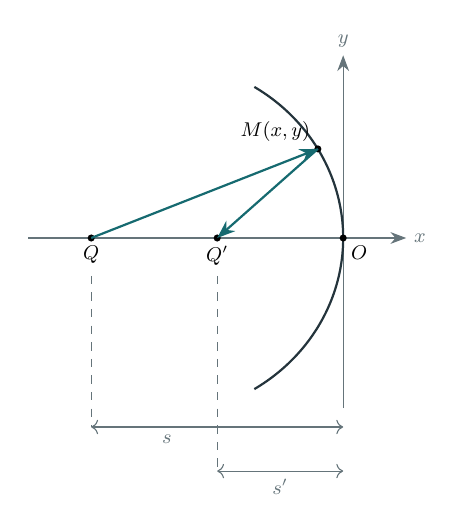
\begin{tikzpicture}[scale=.8,transform shape]

\draw[axis] (-5,0)--(1,0) node[right] {$x$};
\draw[axis] (0,-2.7)--(0,2.9) node[above] {$y$};
\draw[object,domain=-58:58,samples=100] plot ({-3+3*cos(\x)},{2.828427*sin(\x)});
\coordinate (Q) at (-4,0);\coordinate (V) at (-2,0);\coordinate (M) at (-.401924,1.414214);
\fill (Q) circle (1.6pt) node[below] {$Q$};
\fill (V) circle (1.6pt) node[below] {$Q'$};
\fill (0,0) circle (1.6pt) node[below right] {$O$};
\fill (M) circle (1.6pt) node[above left] {$M(x,y)$};
\draw[motion] (Q)--(M);\draw[motion] (M)--(V);
\draw[guide] (-4,-.6)--(-4,-3);\draw[guide] (-2,-.6)--(-2,-3.7);
\draw[axis,<->] (-4,-3)--(0,-3) node[pos=.3,below] {$s$};
\draw[axis,<->] (-2,-3.7)--(0,-3.7) node[midway,below] {$s'$};

\end{tikzpicture}
\figcaption{图光试.1\quad 两有限共轭点在顶点同侧，落到凹面上的光线反射后会聚。}
\end{minipage}\end{center}

\Needspace{8\baselineskip}

\pdfbookmark[3]{题型定位}{q1-h0}

\subsection*{题型定位}

这是由有限共轭点反求无像差反射面的题。费马原理先给镜面切向光程变化为零，连通性再把驻值条件连成一个等光程面。保留两次消根和逐步配方，最后用距离梯度确定法线及出射方向，几何椭圆和实际反射由同一条件贯穿。

\Needspace{8\baselineskip}

\pdfbookmark[3]{知识点}{q1-h1}

\subsection*{知识点}

均匀介质中光程与几何路程成正比。距离和的梯度垂直镜面，连通面上相同的常量由顶点确定。椭圆长短半轴满足$a=D/2$、$b^2=ss'$，焦距半长满足$c^2=a^2-b^2$。平方时保留未平方根式的非负号，距离梯度再把两射线切向分量相等与法向分量相反联系起来。

\Needspace{8\baselineskip}

\pdfbookmark[3]{物理图像}{q1-h2}

\subsection*{物理图像}

图光试.1将$Q,Q'$放在顶点同侧，每条反射路径由$QM$与$MQ'$两段组成。解图光试.1A标出椭圆的中心、半轴和两焦点，图B在反射点$M$画出法线与两单位方向。三维方程只含$y^2+z^2$，对应旋转椭球；实际凹镜取顶点附近所需的一片曲面。

\Needspace{8\baselineskip}

\pdfbookmark[3]{解题入口}{q1-h3}

\subsection*{解题入口}

在反射点$M$写距离和，求沿镜面切向微移的一阶变化，再由连通性与顶点得到常量$D=s+s'$。消根先得到$\sqrt{(x+s')^2+y^2}=s'-\eta x$，再平方、配方。求得半轴后算出两焦点，说明根式右端在整个椭圆上非负，最后用梯度证明反射方向指向$Q'$。

\Needspace{8\baselineskip}

\pdfbookmark[3]{标准解法}{q1-h4}

\subsection*{标准解法}


图光试.1取反射点$M=(x,y)$。均匀介质中的光程与几何路程成正比，略去公共折射率，令
\[
\mathcal L(M)=|QM|+|MQ'|
=\sqrt{(x+s)^2+y^2}+\sqrt{(x+s')^2+y^2}.
\]
费马原理要求光线在反射点沿镜面的微小移动不改变一阶光程，即对任一镜面切向位移$d\boldsymbol r$有
$d\mathcal L=\nabla\mathcal L\cdot d\boldsymbol r=0$。因镜面连通，$\mathcal L$在这片反射面上为常量。顶点$O$给出常量$s+s'$，故
\[
\boxed{\sqrt{(x+s)^2+y^2}+\sqrt{(x+s')^2+y^2}=s+s'}.
\]
\begin{center}\begin{minipage}{.98\linewidth}\centering
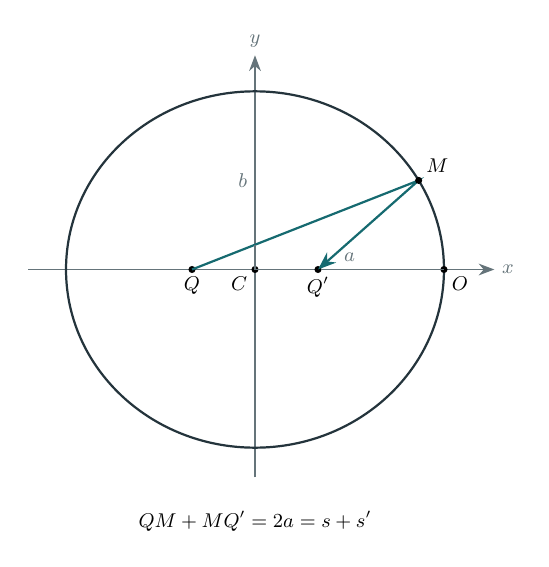
\begin{tikzpicture}[scale=.8,transform shape]

\draw[axis] (-6.6,0)--(.8,0) node[right] {$x$};
\draw[axis] (-3,-3.3)--(-3,3.4) node[above] {$y$};
\draw[object] (-3,0) ellipse (3 and 2.828427);
\fill (-4,0) circle (1.6pt) node[below] {$Q$};
\fill (-2,0) circle (1.6pt) node[below] {$Q'$};
\fill (-3,0) circle (1.6pt) node[below left] {$C$};
\fill (0,0) circle (1.6pt) node[below right] {$O$};
\draw[motion] (-4,0)--(-.401924,1.414214)--(-2,0);
\fill (-.401924,1.414214) circle (1.6pt) node[above right] {$M$};
\draw[guide] (-3,0)--(-3,2.828427) node[midway,left] {$b$};
\draw[guide] (-3,0)--(0,0) node[midway,above] {$a$};
\node at (-3,-4) {$QM+MQ'=2a=s+s'$};

\end{tikzpicture}
\figcaption{解图光试.1A\quad 双焦点定义给出椭圆中心与半轴，右端顶点为O。}
\end{minipage}\end{center}
解图光试.1A中两条焦径之和为$2a=s+s'$。为把几何条件化成直角坐标方程，记$D=s+s'$、$\eta=(s-s')/D$，先移项一次平方：
\[
\begin{aligned}
(x+s)^2+y^2
&=D^2+(x+s')^2+y^2
-2D\sqrt{(x+s')^2+y^2},\\
(s-s')x&=s'D-D\sqrt{(x+s')^2+y^2},\\
\sqrt{(x+s')^2+y^2}&=s'-\eta x.
\end{aligned}
\]
再平方并整理，
\[
(x+s')^2+y^2=(s'-\eta x)^2,
\]
\[
\frac{4ss'}{D^2}x^2+\frac{4ss'}D x+y^2=0.
\]
先除以$4ss'$，再将$x$的线性项配成平方：
\[
\frac{x^2}{D^2}+\frac{x}{D}+\frac{y^2}{4ss'}=0,
\qquad
\left(\frac{x}{D}+\frac12\right)^2+\frac{y^2}{4ss'}=\frac14.
\]
乘回$D^2$，即$(x+D/2)^2+D^2y^2/(4ss')=D^2/4$，因而得到
\[
\boxed{\frac{(x+D/2)^2}{(D/2)^2}+\frac{y^2}{ss'}=1}.
\]
所以截线为椭圆，中心和半轴分别为
\[
\boxed{C=(-D/2,0),\qquad a=D/2,\qquad b=\sqrt{ss'}}.
\]
由$a^2-b^2=(s-s')^2/4$，焦距半长$c=|s-s'|/2$，两个焦点恰为$Q,Q'$。椭圆上$-D\le x\le0$，而未平方关系中的
$s'-\eta x$在两端分别为$s$和$s'$，全段非负，因此整个椭圆都满足两段距离之和为$D$。所用凹镜取椭圆靠近$O$的一段，三维取对应的旋转面片。
\begin{center}\begin{minipage}{.98\linewidth}\centering
\begin{tikzpicture}[scale=.8,transform shape]

\draw[axis] (-5,0)--(1,0) node[right] {$x$};
\draw[axis] (0,-2.7)--(0,2.9) node[above] {$y$};
\draw[object,domain=-58:58,samples=100] plot ({-3+3*cos(\x)},{2.828427*sin(\x)});
\coordinate (Q) at (-4,0);\coordinate (V) at (-2,0);\coordinate (M) at (-.401924,1.414214);
\fill (Q) circle (1.6pt) node[below] {$Q$};
\fill (V) circle (1.6pt) node[below] {$Q'$};
\fill (0,0) circle (1.6pt) node[below right] {$O$};
\fill (M) circle (1.6pt) node[above left] {$M(x,y)$};
\draw[motion] (Q)--(M);\draw[motion] (M)--(V);
\draw[guide] (-4,-.6)--(-4,-3);\draw[guide] (-2,-.6)--(-2,-3.7);
\draw[axis,<->] (-4,-3)--(0,-3) node[pos=.3,below] {$s$};
\draw[axis,<->] (-2,-3.7)--(0,-3.7) node[midway,below] {$s'$};

\draw[force] (-1.4,.802)--(.95,2.243) node[right] {$\boldsymbol n$};
\draw[guide] (-.9,2.23)--(.1,.59);
\node[align=left] at (-4.5,3.5) {$\boldsymbol n\parallel\boldsymbol u_{\rm in}-\boldsymbol u_{\rm out}$\\两光线切向分量相同};

\end{tikzpicture}
\figcaption{解图光试.1B\quad 距离和梯度为镜面法向，反射光从M指向像点。}
\end{minipage}\end{center}
解图光试.1B中，入射单位向量为
$\boldsymbol u_{\rm in}=(M-Q)/|M-Q|$，反射后指向$Q'$的单位向量为
$\boldsymbol u_{\rm out}=(Q'-M)/|Q'-M|$。距离和的梯度
\[
\nabla\mathcal L=\boldsymbol u_{\rm in}-\boldsymbol u_{\rm out}
\]
沿镜面法向，所以两条射线的切向分量相同。在线段 $QQ^\prime$ 上，两段距离的和为 $|s-s^\prime|<D$。这个线段包含距离梯度可能相消的全部位置。镜面上两段距离和为 $D$，因此 $\nabla\mathcal L$ 给出非零法向。两个单位方向彼此不同，模均为1、切向分量相同。由单位长度关系，两者法向分量的平方相等；彼此不同又使其法向分量取相反号，因而给出入射角等于反射角。反射方向因而由$M$指向$Q'$。

三维情况下只将$y^2$换成$y^2+z^2$：
\[
\boxed{\frac{(x+D/2)^2}{(D/2)^2}+\frac{y^2+z^2}{ss'}=1}.
\]
距离和本身对$x$轴旋转不变，因而得到旋转椭球面。若$s=s'$，则$a=b=s$，曲面成为以$Q=Q'$为中心的球面，光线沿径向反射返回。


\Needspace{8\baselineskip}

\pdfbookmark[3]{关键洞察}{q1-h5}

\subsection*{关键洞察}

旋转对称的支撑曲面来自距离和的等值面，推导起点只需指定两个共轭点和连通光滑反射片。该椭球针对这对$Q,Q'$精确等光程；改变端点后，新的距离函数随镜面位置变化。局部顶点曲率给相同的傍轴镜公式，有限孔径的高阶面形则由这对焦点决定。

\Needspace{8\baselineskip}

\pdfbookmark[3]{易错点}{q1-h6}

\subsection*{易错点}

$Q,Q'$在顶点同侧，反射光程使用两距离之和。费马条件对镜面切向变分成立，连通性与顶点共同确定等光程常量。长半轴为距离和的一半；消根后的$-D\leqslant x\leqslant0$使根式右端保持非负。距离梯度不仅确定椭圆法线，也选出由$M$指向$Q'$的实际反射方向。

\Needspace{8\baselineskip}

\pdfbookmark[3]{课堂讲解建议}{q1-h7}

\subsection*{课堂讲解建议}

先在图上标出顶点路程$s+s'$，再让学生写另一个反射点的切向一阶变化。把两次平方与配方分开写，每次保留上一行的根式和符号；得到半轴后由$a^2-b^2$算出焦点。最后取$s=s'$解释径向返回，再比较椭球与相同顶点曲率球面的高阶面形，说明指定焦点对怎样进入有限孔径成像。

\Needspace{8\baselineskip}

\pdfbookmark[3]{变式训练}{q1-h8}

\subsection*{变式训练}

\begin{enumerate}
\Needspace{37\baselineskip}
\item \textbf{三比一共轭距离。}令$s=3s'$、$s'=h$，求完整椭圆参数，并取反射点$y=h$求其顶点侧横坐标和两段路程。

距离和$D=4h$，所以$a=2h$、$b=\sqrt3h$、$c=h$，中心为$(-2h,0)$，两焦点为$(-3h,0)$与$(-h,0)$。在顶点侧分支
\[
x=-2h+2h\sqrt{1-\frac{y^2}{3h^2}},
\quad y=h\ \Longrightarrow\ x=-0.36700684h.
\]
由主解未平方关系$MQ'=h-x/2$，得$MQ'=1.18350342h$，$QM=4h-MQ'=2.81649658h$。图V1将这点与两焦点连起，长度和仍为$4h$，法线由两单位方向之差给出。
\begin{center}\begin{minipage}{.98\linewidth}\centering
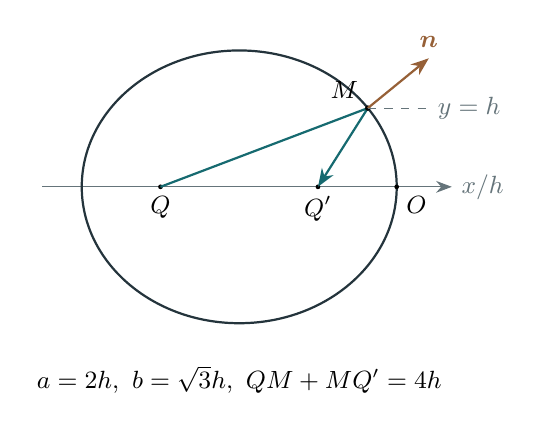
\begin{tikzpicture}[scale=1,transform shape]
\draw[axis] (-4.5,0)--(.7,0) node[right] {$x/h$};\draw[object] (-2,0) ellipse (2 and 1.732050808);
\fill (-3,0) circle(.03) node[below] {$Q$};\fill (-1,0) circle(.03) node[below] {$Q'$};\fill (0,0) circle(.03) node[below right] {$O$};
\draw[motion] (-3,0)--(-0.367006838,1)--(-1,0);\fill (-0.367006838,1) circle(.035) node[above left] {$M$};
\draw[force] (-0.367006838,1)--(0.407589831,1.632455532) node[above] {$\boldsymbol n$};
\draw[guide] (-0.367006838,1)--(.4,1) node[right] {$y=h$};
\node[below] at (-2,-2.15) {$a=2h,\ b=\sqrt3h,\ QM+MQ'=4h$};\end{tikzpicture}
\figcaption{解图光试.1V1\quad 三比一共轭距离的椭圆与反射点M}
\end{minipage}\end{center}
\Needspace{37\baselineskip}
\item \textbf{顶点曲率与高阶面形。}求椭圆顶点曲率半径与局部傍轴焦距，再比较同一顶点曲率球面和椭圆的四阶面形项。

顶点侧面形为$x_e=-a+a\sqrt{1-y^2/b^2}$，展开得
\[
x_e=-\frac{a}{2b^2}y^2-\frac{a}{8b^4}y^4+O(y^6),
\quad R_v=\frac{b^2}{a}=\frac{2ss'}{s+s'},
\quad f_v=\frac{R_v}{2}=\frac{ss'}{s+s'}.
\]
故$1/s+1/s'=1/f_v$。同曲率球面$x_s=-R_v+\sqrt{R_v^2-y^2}$的二阶项相同，而
\[
x_s-x_e=-\frac{(s+s')(s-s')^2}{64s^3s'^3}y^4+O(y^6).
\]
图V2取$s=3h,s'=h$比较两种面形。指定的有限共轭点决定四阶及更高阶曲率变化；$s=s'$时差项归零，整个椭圆成为圆。
\begin{center}\begin{minipage}{.98\linewidth}\centering
\begin{tikzpicture}[scale=0.72,transform shape]
\draw[axis] (0,0)--(6.2,0);\draw[axis] (0,0)--(0,3.4000000000000004);
\draw[thin,color=muted] (0.0000000,0)--(0.0000000,-.07);\node[below] at (0.0000000,-.09) {$0$};
\draw[thin,color=muted] (3.0000000,0)--(3.0000000,-.07);\node[below] at (3.0000000,-.09) {$1/2$};
\draw[thin,color=muted] (6.0000000,0)--(6.0000000,-.07);\node[below] at (6.0000000,-.09) {$1$};
\draw[thin,color=muted] (0,0.3404255)--(-.07,0.3404255);\node[left] at (-.09,0.3404255) {$-.4$};
\draw[thin,color=muted] (0,1.7021277)--(-.07,1.7021277);\node[left] at (-.09,1.7021277) {$-.2$};
\draw[thin,color=muted] (0,3.0638298)--(-.07,3.0638298);\node[left] at (-.09,3.0638298) {$0$};
\node[below] at (3.0,-.64) {$y/h$};\node[above right] at (0,3.45) {面形$x/h$};
\draw[traj] plot coordinates {(0.0000000,3.0638298) (0.0250000,3.0637904) (0.0500000,3.0636722) (0.0750000,3.0634752) (0.1000000,3.0631994) (0.1250000,3.0628447) (0.1500000,3.0624113) (0.1750000,3.0618990) (0.2000000,3.0613079) (0.2250000,3.0606379) (0.2500000,3.0598891) (0.2750000,3.0590614) (0.3000000,3.0581548) (0.3250000,3.0571694) (0.3500000,3.0561050) (0.3750000,3.0549617) (0.4000000,3.0537394) (0.4250000,3.0524381) (0.4500000,3.0510578) (0.4750000,3.0495986) (0.5000000,3.0480602) (0.5250000,3.0464428) (0.5500000,3.0447463) (0.5750000,3.0429706) (0.6000000,3.0411158) (0.6250000,3.0391818) (0.6500000,3.0371685) (0.6750000,3.0350760) (0.7000000,3.0329042) (0.7250000,3.0306530) (0.7500000,3.0283225) (0.7750000,3.0259125) (0.8000000,3.0234231) (0.8250000,3.0208542) (0.8500000,3.0182057) (0.8750000,3.0154776) (0.9000000,3.0126699) (0.9250000,3.0097824) (0.9500000,3.0068152) (0.9750000,3.0037683) (1.0000000,3.0006414) (1.0250000,2.9974347) (1.0500000,2.9941480) (1.0750000,2.9907812) (1.1000000,2.9873344) (1.1250000,2.9838074) (1.1500000,2.9802002) (1.1750000,2.9765128) (1.2000000,2.9727450) (1.2250000,2.9688968) (1.2500000,2.9649682) (1.2750000,2.9609589) (1.3000000,2.9568691) (1.3250000,2.9526986) (1.3500000,2.9484473) (1.3750000,2.9441152) (1.4000000,2.9397022) (1.4250000,2.9352081) (1.4500000,2.9306330) (1.4750000,2.9259768) (1.5000000,2.9212392) (1.5250000,2.9164204) (1.5500000,2.9115201) (1.5750000,2.9065384) (1.6000000,2.9014750) (1.6250000,2.8963299) (1.6500000,2.8911031) (1.6750000,2.8857944) (1.7000000,2.8804037) (1.7250000,2.8749309) (1.7500000,2.8693760) (1.7750000,2.8637387) (1.8000000,2.8580191) (1.8250000,2.8522170) (1.8500000,2.8463324) (1.8750000,2.8403650) (1.9000000,2.8343148) (1.9250000,2.8281817) (1.9500000,2.8219655) (1.9750000,2.8156662) (2.0000000,2.8092836) (2.0250000,2.8028176) (2.0500000,2.7962681) (2.0750000,2.7896350) (2.1000000,2.7829181) (2.1250000,2.7761173) (2.1500000,2.7692325) (2.1750000,2.7622636) (2.2000000,2.7552103) (2.2250000,2.7480727) (2.2500000,2.7408505) (2.2750000,2.7335436) (2.3000000,2.7261519) (2.3250000,2.7186753) (2.3500000,2.7111135) (2.3750000,2.7034665) (2.4000000,2.6957340) (2.4250000,2.6879160) (2.4500000,2.6800123) (2.4750000,2.6720228) (2.5000000,2.6639472) (2.5250000,2.6557855) (2.5500000,2.6475374) (2.5750000,2.6392028) (2.6000000,2.6307816) (2.6250000,2.6222735) (2.6500000,2.6136784) (2.6750000,2.6049962) (2.7000000,2.5962267) (2.7250000,2.5873696) (2.7500000,2.5784248) (2.7750000,2.5693922) (2.8000000,2.5602715) (2.8250000,2.5510626) (2.8500000,2.5417653) (2.8750000,2.5323794) (2.9000000,2.5229046) (2.9250000,2.5133409) (2.9500000,2.5036880) (2.9750000,2.4939457) (3.0000000,2.4841138) (3.0250000,2.4741921) (3.0500000,2.4641805) (3.0750000,2.4540786) (3.1000000,2.4438863) (3.1250000,2.4336034) (3.1500000,2.4232297) (3.1750000,2.4127648) (3.2000000,2.4022088) (3.2250000,2.3915612) (3.2500000,2.3808219) (3.2750000,2.3699906) (3.3000000,2.3590671) (3.3250000,2.3480512) (3.3500000,2.3369427) (3.3750000,2.3257412) (3.4000000,2.3144466) (3.4250000,2.3030587) (3.4500000,2.2915771) (3.4750000,2.2800016) (3.5000000,2.2683319) (3.5250000,2.2565679) (3.5500000,2.2447092) (3.5750000,2.2327556) (3.6000000,2.2207068) (3.6250000,2.2085625) (3.6500000,2.1963225) (3.6750000,2.1839865) (3.7000000,2.1715542) (3.7250000,2.1590253) (3.7500000,2.1463996) (3.7750000,2.1336767) (3.8000000,2.1208564) (3.8250000,2.1079384) (3.8500000,2.0949223) (3.8750000,2.0818079) (3.9000000,2.0685949) (3.9250000,2.0552829) (3.9500000,2.0418716) (3.9750000,2.0283608) (4.0000000,2.0147501) (4.0250000,2.0010391) (4.0500000,1.9872275) (4.0750000,1.9733151) (4.1000000,1.9593015) (4.1250000,1.9451863) (4.1500000,1.9309691) (4.1750000,1.9166497) (4.2000000,1.9022277) (4.2250000,1.8877028) (4.2500000,1.8730745) (4.2750000,1.8583425) (4.3000000,1.8435064) (4.3250000,1.8285659) (4.3500000,1.8135205) (4.3750000,1.7983700) (4.4000000,1.7831139) (4.4250000,1.7677518) (4.4500000,1.7522833) (4.4750000,1.7367081) (4.5000000,1.7210256) (4.5250000,1.7052356) (4.5500000,1.6893375) (4.5750000,1.6733310) (4.6000000,1.6572157) (4.6250000,1.6409910) (4.6500000,1.6246566) (4.6750000,1.6082121) (4.7000000,1.5916569) (4.7250000,1.5749907) (4.7500000,1.5582129) (4.7750000,1.5413231) (4.8000000,1.5243209) (4.8250000,1.5072057) (4.8500000,1.4899771) (4.8750000,1.4726345) (4.9000000,1.4551776) (4.9250000,1.4376058) (4.9500000,1.4199186) (4.9750000,1.4021154) (5.0000000,1.3841958) (5.0250000,1.3661592) (5.0500000,1.3480052) (5.0750000,1.3297331) (5.1000000,1.3113424) (5.1250000,1.2928326) (5.1500000,1.2742031) (5.1750000,1.2554533) (5.2000000,1.2365827) (5.2250000,1.2175907) (5.2500000,1.1984767) (5.2750000,1.1792401) (5.3000000,1.1598803) (5.3250000,1.1403966) (5.3500000,1.1207886) (5.3750000,1.1010554) (5.4000000,1.0811966) (5.4250000,1.0612114) (5.4500000,1.0410992) (5.4750000,1.0208594) (5.5000000,1.0004912) (5.5250000,0.9799941) (5.5500000,0.9593672) (5.5750000,0.9386099) (5.6000000,0.9177215) (5.6250000,0.8967013) (5.6500000,0.8755486) (5.6750000,0.8542625) (5.7000000,0.8328424) (5.7250000,0.8112876) (5.7500000,0.7895971) (5.7750000,0.7677703) (5.8000000,0.7458064) (5.8250000,0.7237046) (5.8500000,0.7014640) (5.8750000,0.6790838) (5.9000000,0.6565633) (5.9250000,0.6339015) (5.9500000,0.6110975) (5.9750000,0.5881506) (6.0000000,0.5650598)};
\draw[traj] (.1,-1.08)--(.7,-1.08);\node[right] at (.85,-1.08) {椭圆$x_e/h$};\draw[dashed,thick,color=warm] plot coordinates {(0.0000000,3.0638298) (0.0250000,3.0637904) (0.0500000,3.0636722) (0.0750000,3.0634752) (0.1000000,3.0631994) (0.1250000,3.0628447) (0.1500000,3.0624112) (0.1750000,3.0618990) (0.2000000,3.0613078) (0.2250000,3.0606378) (0.2500000,3.0598889) (0.2750000,3.0590611) (0.3000000,3.0581545) (0.3250000,3.0571688) (0.3500000,3.0561042) (0.3750000,3.0549607) (0.4000000,3.0537381) (0.4250000,3.0524365) (0.4500000,3.0510558) (0.4750000,3.0495961) (0.5000000,3.0480572) (0.5250000,3.0464391) (0.5500000,3.0447418) (0.5750000,3.0429653) (0.6000000,3.0411095) (0.6250000,3.0391743) (0.6500000,3.0371598) (0.6750000,3.0350659) (0.7000000,3.0328925) (0.7250000,3.0306395) (0.7500000,3.0283070) (0.7750000,3.0258949) (0.8000000,3.0234030) (0.8250000,3.0208315) (0.8500000,3.0181801) (0.8750000,3.0154488) (0.9000000,3.0126377) (0.9250000,3.0097465) (0.9500000,3.0067752) (0.9750000,3.0037238) (1.0000000,3.0005922) (1.0250000,2.9973804) (1.0500000,2.9940881) (1.0750000,2.9907154) (1.1000000,2.9872622) (1.1250000,2.9837284) (1.1500000,2.9801139) (1.1750000,2.9764187) (1.2000000,2.9726426) (1.2250000,2.9687855) (1.2500000,2.9648474) (1.2750000,2.9608281) (1.3000000,2.9567276) (1.3250000,2.9525458) (1.3500000,2.9482825) (1.3750000,2.9439377) (1.4000000,2.9395113) (1.4250000,2.9350031) (1.4500000,2.9304130) (1.4750000,2.9257410) (1.5000000,2.9209869) (1.5250000,2.9161505) (1.5500000,2.9112319) (1.5750000,2.9062308) (1.6000000,2.9011472) (1.6250000,2.8959808) (1.6500000,2.8907316) (1.6750000,2.8853995) (1.7000000,2.8799843) (1.7250000,2.8744859) (1.7500000,2.8689042) (1.7750000,2.8632389) (1.8000000,2.8574900) (1.8250000,2.8516573) (1.8500000,2.8457407) (1.8750000,2.8397401) (1.9000000,2.8336552) (1.9250000,2.8274859) (1.9500000,2.8212321) (1.9750000,2.8148936) (2.0000000,2.8084702) (2.0250000,2.8019618) (2.0500000,2.7953683) (2.0750000,2.7886893) (2.1000000,2.7819249) (2.1250000,2.7750747) (2.1500000,2.7681386) (2.1750000,2.7611165) (2.2000000,2.7540082) (2.2250000,2.7468134) (2.2500000,2.7395319) (2.2750000,2.7321637) (2.3000000,2.7247085) (2.3250000,2.7171660) (2.3500000,2.7095362) (2.3750000,2.7018187) (2.4000000,2.6940135) (2.4250000,2.6861202) (2.4500000,2.6781387) (2.4750000,2.6700687) (2.5000000,2.6619101) (2.5250000,2.6536625) (2.5500000,2.6453259) (2.5750000,2.6368999) (2.6000000,2.6283843) (2.6250000,2.6197790) (2.6500000,2.6110836) (2.6750000,2.6022979) (2.7000000,2.5934216) (2.7250000,2.5844546) (2.7500000,2.5753966) (2.7750000,2.5662473) (2.8000000,2.5570064) (2.8250000,2.5476738) (2.8500000,2.5382490) (2.8750000,2.5287320) (2.9000000,2.5191223) (2.9250000,2.5094197) (2.9500000,2.4996240) (2.9750000,2.4897348) (3.0000000,2.4797519) (3.0250000,2.4696750) (3.0500000,2.4595037) (3.0750000,2.4492378) (3.1000000,2.4388770) (3.1250000,2.4284209) (3.1500000,2.4178693) (3.1750000,2.4072218) (3.2000000,2.3964781) (3.2250000,2.3856379) (3.2500000,2.3747009) (3.2750000,2.3636667) (3.3000000,2.3525350) (3.3250000,2.3413054) (3.3500000,2.3299776) (3.3750000,2.3185513) (3.4000000,2.3070260) (3.4250000,2.2954015) (3.4500000,2.2836773) (3.4750000,2.2718531) (3.5000000,2.2599285) (3.5250000,2.2479031) (3.5500000,2.2357766) (3.5750000,2.2235485) (3.6000000,2.2112184) (3.6250000,2.1987860) (3.6500000,2.1862509) (3.6750000,2.1736125) (3.7000000,2.1608706) (3.7250000,2.1480246) (3.7500000,2.1350741) (3.7750000,2.1220188) (3.8000000,2.1088581) (3.8250000,2.0955917) (3.8500000,2.0822189) (3.8750000,2.0687395) (3.9000000,2.0551529) (3.9250000,2.0414587) (3.9500000,2.0276563) (3.9750000,2.0137452) (4.0000000,1.9997251) (4.0250000,1.9855953) (4.0500000,1.9713555) (4.0750000,1.9570049) (4.1000000,1.9425432) (4.1250000,1.9279698) (4.1500000,1.9132841) (4.1750000,1.8984857) (4.2000000,1.8835739) (4.2250000,1.8685482) (4.2500000,1.8534080) (4.2750000,1.8381528) (4.3000000,1.8227819) (4.3250000,1.8072948) (4.3500000,1.7916909) (4.3750000,1.7759695) (4.4000000,1.7601300) (4.4250000,1.7441718) (4.4500000,1.7280943) (4.4750000,1.7118968) (4.5000000,1.6955786) (4.5250000,1.6791391) (4.5500000,1.6625776) (4.5750000,1.6458934) (4.6000000,1.6290858) (4.6250000,1.6121541) (4.6500000,1.5950976) (4.6750000,1.5779155) (4.7000000,1.5606071) (4.7250000,1.5431717) (4.7500000,1.5256084) (4.7750000,1.5079166) (4.8000000,1.4900953) (4.8250000,1.4721439) (4.8500000,1.4540615) (4.8750000,1.4358472) (4.9000000,1.4175003) (4.9250000,1.3990198) (4.9500000,1.3804050) (4.9750000,1.3616548) (5.0000000,1.3427685) (5.0250000,1.3237451) (5.0500000,1.3045837) (5.0750000,1.2852834) (5.1000000,1.2658431) (5.1250000,1.2462620) (5.1500000,1.2265390) (5.1750000,1.2066731) (5.2000000,1.1866633) (5.2250000,1.1665086) (5.2500000,1.1462080) (5.2750000,1.1257602) (5.3000000,1.1051643) (5.3250000,1.0844191) (5.3500000,1.0635236) (5.3750000,1.0424764) (5.4000000,1.0212766) (5.4250000,0.9999228) (5.4500000,0.9784140) (5.4750000,0.9567487) (5.5000000,0.9349259) (5.5250000,0.9129441) (5.5500000,0.8908022) (5.5750000,0.8684987) (5.6000000,0.8460323) (5.6250000,0.8234017) (5.6500000,0.8006054) (5.6750000,0.7776421) (5.7000000,0.7545101) (5.7250000,0.7312082) (5.7500000,0.7077347) (5.7750000,0.6840881) (5.8000000,0.6602669) (5.8250000,0.6362694) (5.8500000,0.6120940) (5.8750000,0.5877391) (5.9000000,0.5632029) (5.9250000,0.5384837) (5.9500000,0.5135797) (5.9750000,0.4884891) (6.0000000,0.4632101)};
\draw[dashed,thick,color=warm] (.1,-1.51)--(.7,-1.51);\node[right] at (.85,-1.51) {同曲率球面$x_s/h$};\end{tikzpicture}
\figcaption{解图光试.1V2\quad 二阶面形相同，球面与椭圆的差别从四阶开始}
\end{minipage}\end{center}
\Needspace{37\baselineskip}
\item \textbf{远像点的抛物面极限。}保持物点$Q=(-s,0)$，令像点距离$s'\to\infty$，求顶点附近的曲面极限，并由可逆性说明反向成像。

对有限$x,y$，远焦径为$\sqrt{(x+s')^2+y^2}=s'+x+O(1/s')$。距离和减去$s'$后变为
\[
\sqrt{(x+s)^2+y^2}=s-x.
\]
平方得$y^2=-4sx$，三维为$y^2+z^2=-4sx$。图V3中从焦点$(-s,0)$出发的光反射为沿$-x$的平行光；逆向平行光沿同一路径反射到该焦点。顶点曲率半径趋于$2s$，局部焦距趋于$s$，与此精确抛物面结果相连。
\begin{center}\begin{minipage}{.98\linewidth}\centering
\begin{tikzpicture}[scale=1,transform shape]
\draw[axis] (-3,0)--(.6,0) node[right] {$x/s$};\draw[object,domain=-1.5:1.5,samples=101] plot ({-\x*\x/4},{\x});\fill (-1,0) circle(.03) node[below] {$Q$};\fill (0,0) circle(.03) node[below right] {$O$};\draw[motion] (-1,0)--(-0.36,-1.2);\draw[force] (-0.36,-1.2)--(-2.8,-1.2);\draw[motion] (-1,0)--(-0.16000000000000003,-0.8);\draw[force] (-0.16000000000000003,-0.8)--(-2.8,-0.8);\draw[motion] (-1,0)--(-0.16000000000000003,0.8);\draw[force] (-0.16000000000000003,0.8)--(-2.8,0.8);\draw[motion] (-1,0)--(-0.36,1.2);\draw[force] (-0.36,1.2)--(-2.8,1.2);\node[above] at (-1.2,1.9) {$y^2=-4sx$};\node[below] at (-1.3,-1.9) {焦点发出的光反射为沿$-x$的平行光};\end{tikzpicture}
\figcaption{解图光试.1V3\quad 远像点极限为抛物面，反向平行光聚于Q}
\end{minipage}\end{center}
\Needspace{37\baselineskip}
\item \textbf{共同相位与二次相位。}周围为空气，在镜面额外赋予等效光程$\delta\mathcal L=C+\alpha y^2$，其中$\alpha$的单位为长度的倒数，采用小孔径近轴近似。比较共同常量$C$与二次项对成像的作用，求新傍轴像距。

共同常量使所有反射点相位增加同一个$2\pi C/\lambda$，光程切向导数保持不变。二次项的导数为$2\alpha y$。若新的像距为$s'_{\rm eff}$，将镜面二阶项$x=-y^2/(2R_v)$代入两段几何路程，$y^2$的系数为
\[
-\frac1{R_v}+\frac1{2s}+\frac1{2s'_{\rm eff}}+\alpha.
\]
用原有$2/R_v=1/s+1/s'$，费马条件给
\[
\frac1{s'_{\rm eff}}=\frac1{s'}-2\alpha.
\]
图V4画出该二阶系数随新像方光焦度的变化。取$\alpha=1/(4s')$时，新傍轴像距为$2s'$；共同相位保持成像方向，位置的二次相位则改变傍轴像距。
\begin{center}\begin{minipage}{.98\linewidth}\centering
\begin{tikzpicture}[scale=0.72,transform shape]
\draw[axis] (0,0)--(6.2,0);\draw[axis] (0,0)--(0,3.4000000000000004);
\draw[thin,color=muted] (0.0000000,0)--(0.0000000,-.07);\node[below] at (0.0000000,-.09) {$0$};
\draw[thin,color=muted] (2.0000000,0)--(2.0000000,-.07);\node[below] at (2.0000000,-.09) {$1/2$};
\draw[thin,color=muted] (4.0000000,0)--(4.0000000,-.07);\node[below] at (4.0000000,-.09) {$1$};
\draw[thin,color=muted] (6.0000000,0)--(6.0000000,-.07);\node[below] at (6.0000000,-.09) {$3/2$};
\draw[thin,color=muted] (0,0.1391304)--(-.07,0.1391304);\node[left] at (-.09,0.1391304) {$-1/2$};
\draw[thin,color=muted] (0,1.5304348)--(-.07,1.5304348);\node[left] at (-.09,1.5304348) {$0$};
\draw[thin,color=muted] (0,2.9217391)--(-.07,2.9217391);\node[left] at (-.09,2.9217391) {$1/2$};
\node[below] at (3.0,-.64) {$z=s^\prime/s^\prime_{\rm eff}$};\node[above right] at (0,3.45) {$s^\prime\times y^2$的系数};
\draw[traj] plot coordinates {(0.0000000,0.1391304) (0.0250000,0.1478261) (0.0500000,0.1565217) (0.0750000,0.1652174) (0.1000000,0.1739130) (0.1250000,0.1826087) (0.1500000,0.1913043) (0.1750000,0.2000000) (0.2000000,0.2086957) (0.2250000,0.2173913) (0.2500000,0.2260870) (0.2750000,0.2347826) (0.3000000,0.2434783) (0.3250000,0.2521739) (0.3500000,0.2608696) (0.3750000,0.2695652) (0.4000000,0.2782609) (0.4250000,0.2869565) (0.4500000,0.2956522) (0.4750000,0.3043478) (0.5000000,0.3130435) (0.5250000,0.3217391) (0.5500000,0.3304348) (0.5750000,0.3391304) (0.6000000,0.3478261) (0.6250000,0.3565217) (0.6500000,0.3652174) (0.6750000,0.3739130) (0.7000000,0.3826087) (0.7250000,0.3913043) (0.7500000,0.4000000) (0.7750000,0.4086957) (0.8000000,0.4173913) (0.8250000,0.4260870) (0.8500000,0.4347826) (0.8750000,0.4434783) (0.9000000,0.4521739) (0.9250000,0.4608696) (0.9500000,0.4695652) (0.9750000,0.4782609) (1.0000000,0.4869565) (1.0250000,0.4956522) (1.0500000,0.5043478) (1.0750000,0.5130435) (1.1000000,0.5217391) (1.1250000,0.5304348) (1.1500000,0.5391304) (1.1750000,0.5478261) (1.2000000,0.5565217) (1.2250000,0.5652174) (1.2500000,0.5739130) (1.2750000,0.5826087) (1.3000000,0.5913043) (1.3250000,0.6000000) (1.3500000,0.6086957) (1.3750000,0.6173913) (1.4000000,0.6260870) (1.4250000,0.6347826) (1.4500000,0.6434783) (1.4750000,0.6521739) (1.5000000,0.6608696) (1.5250000,0.6695652) (1.5500000,0.6782609) (1.5750000,0.6869565) (1.6000000,0.6956522) (1.6250000,0.7043478) (1.6500000,0.7130435) (1.6750000,0.7217391) (1.7000000,0.7304348) (1.7250000,0.7391304) (1.7500000,0.7478261) (1.7750000,0.7565217) (1.8000000,0.7652174) (1.8250000,0.7739130) (1.8500000,0.7826087) (1.8750000,0.7913043) (1.9000000,0.8000000) (1.9250000,0.8086957) (1.9500000,0.8173913) (1.9750000,0.8260870) (2.0000000,0.8347826) (2.0250000,0.8434783) (2.0500000,0.8521739) (2.0750000,0.8608696) (2.1000000,0.8695652) (2.1250000,0.8782609) (2.1500000,0.8869565) (2.1750000,0.8956522) (2.2000000,0.9043478) (2.2250000,0.9130435) (2.2500000,0.9217391) (2.2750000,0.9304348) (2.3000000,0.9391304) (2.3250000,0.9478261) (2.3500000,0.9565217) (2.3750000,0.9652174) (2.4000000,0.9739130) (2.4250000,0.9826087) (2.4500000,0.9913043) (2.4750000,1.0000000) (2.5000000,1.0086957) (2.5250000,1.0173913) (2.5500000,1.0260870) (2.5750000,1.0347826) (2.6000000,1.0434783) (2.6250000,1.0521739) (2.6500000,1.0608696) (2.6750000,1.0695652) (2.7000000,1.0782609) (2.7250000,1.0869565) (2.7500000,1.0956522) (2.7750000,1.1043478) (2.8000000,1.1130435) (2.8250000,1.1217391) (2.8500000,1.1304348) (2.8750000,1.1391304) (2.9000000,1.1478261) (2.9250000,1.1565217) (2.9500000,1.1652174) (2.9750000,1.1739130) (3.0000000,1.1826087) (3.0250000,1.1913043) (3.0500000,1.2000000) (3.0750000,1.2086957) (3.1000000,1.2173913) (3.1250000,1.2260870) (3.1500000,1.2347826) (3.1750000,1.2434783) (3.2000000,1.2521739) (3.2250000,1.2608696) (3.2500000,1.2695652) (3.2750000,1.2782609) (3.3000000,1.2869565) (3.3250000,1.2956522) (3.3500000,1.3043478) (3.3750000,1.3130435) (3.4000000,1.3217391) (3.4250000,1.3304348) (3.4500000,1.3391304) (3.4750000,1.3478261) (3.5000000,1.3565217) (3.5250000,1.3652174) (3.5500000,1.3739130) (3.5750000,1.3826087) (3.6000000,1.3913043) (3.6250000,1.4000000) (3.6500000,1.4086957) (3.6750000,1.4173913) (3.7000000,1.4260870) (3.7250000,1.4347826) (3.7500000,1.4434783) (3.7750000,1.4521739) (3.8000000,1.4608696) (3.8250000,1.4695652) (3.8500000,1.4782609) (3.8750000,1.4869565) (3.9000000,1.4956522) (3.9250000,1.5043478) (3.9500000,1.5130435) (3.9750000,1.5217391) (4.0000000,1.5304348) (4.0250000,1.5391304) (4.0500000,1.5478261) (4.0750000,1.5565217) (4.1000000,1.5652174) (4.1250000,1.5739130) (4.1500000,1.5826087) (4.1750000,1.5913043) (4.2000000,1.6000000) (4.2250000,1.6086957) (4.2500000,1.6173913) (4.2750000,1.6260870) (4.3000000,1.6347826) (4.3250000,1.6434783) (4.3500000,1.6521739) (4.3750000,1.6608696) (4.4000000,1.6695652) (4.4250000,1.6782609) (4.4500000,1.6869565) (4.4750000,1.6956522) (4.5000000,1.7043478) (4.5250000,1.7130435) (4.5500000,1.7217391) (4.5750000,1.7304348) (4.6000000,1.7391304) (4.6250000,1.7478261) (4.6500000,1.7565217) (4.6750000,1.7652174) (4.7000000,1.7739130) (4.7250000,1.7826087) (4.7500000,1.7913043) (4.7750000,1.8000000) (4.8000000,1.8086957) (4.8250000,1.8173913) (4.8500000,1.8260870) (4.8750000,1.8347826) (4.9000000,1.8434783) (4.9250000,1.8521739) (4.9500000,1.8608696) (4.9750000,1.8695652) (5.0000000,1.8782609) (5.0250000,1.8869565) (5.0500000,1.8956522) (5.0750000,1.9043478) (5.1000000,1.9130435) (5.1250000,1.9217391) (5.1500000,1.9304348) (5.1750000,1.9391304) (5.2000000,1.9478261) (5.2250000,1.9565217) (5.2500000,1.9652174) (5.2750000,1.9739130) (5.3000000,1.9826087) (5.3250000,1.9913043) (5.3500000,2.0000000) (5.3750000,2.0086957) (5.4000000,2.0173913) (5.4250000,2.0260870) (5.4500000,2.0347826) (5.4750000,2.0434783) (5.5000000,2.0521739) (5.5250000,2.0608696) (5.5500000,2.0695652) (5.5750000,2.0782609) (5.6000000,2.0869565) (5.6250000,2.0956522) (5.6500000,2.1043478) (5.6750000,2.1130435) (5.7000000,2.1217391) (5.7250000,2.1304348) (5.7500000,2.1391304) (5.7750000,2.1478261) (5.8000000,2.1565217) (5.8250000,2.1652174) (5.8500000,2.1739130) (5.8750000,2.1826087) (5.9000000,2.1913043) (5.9250000,2.2000000) (5.9500000,2.2086957) (5.9750000,2.2173913) (6.0000000,2.2260870)};
\draw[traj] (.1,-1.08)--(.7,-1.08);\node[right] at (.85,-1.08) {$\alpha=0$，零点$z=1$};\draw[dashed,thick,color=warm] plot coordinates {(0.0000000,0.8347826) (0.0250000,0.8434783) (0.0500000,0.8521739) (0.0750000,0.8608696) (0.1000000,0.8695652) (0.1250000,0.8782609) (0.1500000,0.8869565) (0.1750000,0.8956522) (0.2000000,0.9043478) (0.2250000,0.9130435) (0.2500000,0.9217391) (0.2750000,0.9304348) (0.3000000,0.9391304) (0.3250000,0.9478261) (0.3500000,0.9565217) (0.3750000,0.9652174) (0.4000000,0.9739130) (0.4250000,0.9826087) (0.4500000,0.9913043) (0.4750000,1.0000000) (0.5000000,1.0086957) (0.5250000,1.0173913) (0.5500000,1.0260870) (0.5750000,1.0347826) (0.6000000,1.0434783) (0.6250000,1.0521739) (0.6500000,1.0608696) (0.6750000,1.0695652) (0.7000000,1.0782609) (0.7250000,1.0869565) (0.7500000,1.0956522) (0.7750000,1.1043478) (0.8000000,1.1130435) (0.8250000,1.1217391) (0.8500000,1.1304348) (0.8750000,1.1391304) (0.9000000,1.1478261) (0.9250000,1.1565217) (0.9500000,1.1652174) (0.9750000,1.1739130) (1.0000000,1.1826087) (1.0250000,1.1913043) (1.0500000,1.2000000) (1.0750000,1.2086957) (1.1000000,1.2173913) (1.1250000,1.2260870) (1.1500000,1.2347826) (1.1750000,1.2434783) (1.2000000,1.2521739) (1.2250000,1.2608696) (1.2500000,1.2695652) (1.2750000,1.2782609) (1.3000000,1.2869565) (1.3250000,1.2956522) (1.3500000,1.3043478) (1.3750000,1.3130435) (1.4000000,1.3217391) (1.4250000,1.3304348) (1.4500000,1.3391304) (1.4750000,1.3478261) (1.5000000,1.3565217) (1.5250000,1.3652174) (1.5500000,1.3739130) (1.5750000,1.3826087) (1.6000000,1.3913043) (1.6250000,1.4000000) (1.6500000,1.4086957) (1.6750000,1.4173913) (1.7000000,1.4260870) (1.7250000,1.4347826) (1.7500000,1.4434783) (1.7750000,1.4521739) (1.8000000,1.4608696) (1.8250000,1.4695652) (1.8500000,1.4782609) (1.8750000,1.4869565) (1.9000000,1.4956522) (1.9250000,1.5043478) (1.9500000,1.5130435) (1.9750000,1.5217391) (2.0000000,1.5304348) (2.0250000,1.5391304) (2.0500000,1.5478261) (2.0750000,1.5565217) (2.1000000,1.5652174) (2.1250000,1.5739130) (2.1500000,1.5826087) (2.1750000,1.5913043) (2.2000000,1.6000000) (2.2250000,1.6086957) (2.2500000,1.6173913) (2.2750000,1.6260870) (2.3000000,1.6347826) (2.3250000,1.6434783) (2.3500000,1.6521739) (2.3750000,1.6608696) (2.4000000,1.6695652) (2.4250000,1.6782609) (2.4500000,1.6869565) (2.4750000,1.6956522) (2.5000000,1.7043478) (2.5250000,1.7130435) (2.5500000,1.7217391) (2.5750000,1.7304348) (2.6000000,1.7391304) (2.6250000,1.7478261) (2.6500000,1.7565217) (2.6750000,1.7652174) (2.7000000,1.7739130) (2.7250000,1.7826087) (2.7500000,1.7913043) (2.7750000,1.8000000) (2.8000000,1.8086957) (2.8250000,1.8173913) (2.8500000,1.8260870) (2.8750000,1.8347826) (2.9000000,1.8434783) (2.9250000,1.8521739) (2.9500000,1.8608696) (2.9750000,1.8695652) (3.0000000,1.8782609) (3.0250000,1.8869565) (3.0500000,1.8956522) (3.0750000,1.9043478) (3.1000000,1.9130435) (3.1250000,1.9217391) (3.1500000,1.9304348) (3.1750000,1.9391304) (3.2000000,1.9478261) (3.2250000,1.9565217) (3.2500000,1.9652174) (3.2750000,1.9739130) (3.3000000,1.9826087) (3.3250000,1.9913043) (3.3500000,2.0000000) (3.3750000,2.0086957) (3.4000000,2.0173913) (3.4250000,2.0260870) (3.4500000,2.0347826) (3.4750000,2.0434783) (3.5000000,2.0521739) (3.5250000,2.0608696) (3.5500000,2.0695652) (3.5750000,2.0782609) (3.6000000,2.0869565) (3.6250000,2.0956522) (3.6500000,2.1043478) (3.6750000,2.1130435) (3.7000000,2.1217391) (3.7250000,2.1304348) (3.7500000,2.1391304) (3.7750000,2.1478261) (3.8000000,2.1565217) (3.8250000,2.1652174) (3.8500000,2.1739130) (3.8750000,2.1826087) (3.9000000,2.1913043) (3.9250000,2.2000000) (3.9500000,2.2086957) (3.9750000,2.2173913) (4.0000000,2.2260870) (4.0250000,2.2347826) (4.0500000,2.2434783) (4.0750000,2.2521739) (4.1000000,2.2608696) (4.1250000,2.2695652) (4.1500000,2.2782609) (4.1750000,2.2869565) (4.2000000,2.2956522) (4.2250000,2.3043478) (4.2500000,2.3130435) (4.2750000,2.3217391) (4.3000000,2.3304348) (4.3250000,2.3391304) (4.3500000,2.3478261) (4.3750000,2.3565217) (4.4000000,2.3652174) (4.4250000,2.3739130) (4.4500000,2.3826087) (4.4750000,2.3913043) (4.5000000,2.4000000) (4.5250000,2.4086957) (4.5500000,2.4173913) (4.5750000,2.4260870) (4.6000000,2.4347826) (4.6250000,2.4434783) (4.6500000,2.4521739) (4.6750000,2.4608696) (4.7000000,2.4695652) (4.7250000,2.4782609) (4.7500000,2.4869565) (4.7750000,2.4956522) (4.8000000,2.5043478) (4.8250000,2.5130435) (4.8500000,2.5217391) (4.8750000,2.5304348) (4.9000000,2.5391304) (4.9250000,2.5478261) (4.9500000,2.5565217) (4.9750000,2.5652174) (5.0000000,2.5739130) (5.0250000,2.5826087) (5.0500000,2.5913043) (5.0750000,2.6000000) (5.1000000,2.6086957) (5.1250000,2.6173913) (5.1500000,2.6260870) (5.1750000,2.6347826) (5.2000000,2.6434783) (5.2250000,2.6521739) (5.2500000,2.6608696) (5.2750000,2.6695652) (5.3000000,2.6782609) (5.3250000,2.6869565) (5.3500000,2.6956522) (5.3750000,2.7043478) (5.4000000,2.7130435) (5.4250000,2.7217391) (5.4500000,2.7304348) (5.4750000,2.7391304) (5.5000000,2.7478261) (5.5250000,2.7565217) (5.5500000,2.7652174) (5.5750000,2.7739130) (5.6000000,2.7826087) (5.6250000,2.7913043) (5.6500000,2.8000000) (5.6750000,2.8086957) (5.7000000,2.8173913) (5.7250000,2.8260870) (5.7500000,2.8347826) (5.7750000,2.8434783) (5.8000000,2.8521739) (5.8250000,2.8608696) (5.8500000,2.8695652) (5.8750000,2.8782609) (5.9000000,2.8869565) (5.9250000,2.8956522) (5.9500000,2.9043478) (5.9750000,2.9130435) (6.0000000,2.9217391)};
\draw[dashed,thick,color=warm] (.1,-1.51)--(.7,-1.51);\node[right] at (.85,-1.51) {$\alpha s^\prime=1/4$，零点$z=1/2$};\end{tikzpicture}
\figcaption{解图光试.1V4\quad 二次相位移动二阶系数的零点，共同常量相位不改变该曲线}
\end{minipage}\end{center}
\Needspace{37\baselineskip}
\item \textbf{固定焦点的椭圆族。}固定两个焦点$Q,Q'$，允许镜面顶点的位置改变。设镜面上的距离和为给定常量$K>|QQ'|$，求全部共焦椭圆的参数。

两焦点中点仍为$C=(-D/2,0)$，焦距半长$c=|s-s'|/2$保持。新长半轴$a_K=K/2$，短半轴由$b_K^2=a_K^2-c^2$给出，所以
\[
\frac{(x+D/2)^2}{K^2/4}+\frac{y^2}{K^2/4-(s-s')^2/4}=1.
\]
顶点位于$x=-D/2\pm K/2$，仅当$K=D$时其中一端位于$O$。图V5画出同一对焦点对应的三条距离和等值线，每条面片都把$Q$反射到$Q'$，不同的$K$给不同的共同相位。
\begin{center}\begin{minipage}{.98\linewidth}\centering
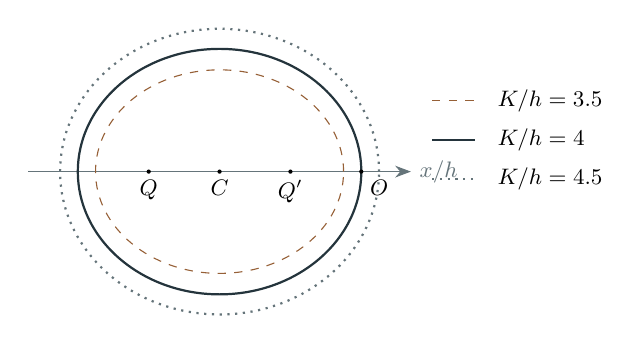
\begin{tikzpicture}[scale=0.9,transform shape]
\draw[axis] (-4.7,0)--(.7,0) node[right] {$x/h$};\draw[dashed,color=warm] (-2,0) ellipse (1.75 and 1.436140662);\draw[dashed,color=warm] (1,1.0)--(1.6,1.0);\node[right] at (1.8,1.0) {$K/h=3.5$};\draw[object] (-2,0) ellipse (2.0 and 1.732050808);\draw[object] (1,0.44999999999999996)--(1.6,0.44999999999999996);\node[right] at (1.8,0.44999999999999996) {$K/h=4$};\draw[dotted,thick,color=muted] (-2,0) ellipse (2.25 and 2.015564437);\draw[dotted,thick,color=muted] (1,-0.10000000000000009)--(1.6,-0.10000000000000009);\node[right] at (1.8,-0.10000000000000009) {$K/h=4.5$};\fill (-3,0) circle(.03) node[below] {$Q$};\fill (-1,0) circle(.03) node[below] {$Q^\prime$};\fill (-2,0) circle(.03) node[below] {$C$};\fill (0,0) circle(.03) node[below right] {$O$};\end{tikzpicture}
\figcaption{解图光试.1V5\quad 固定焦点的距离和等值线，只有K等于4h的一条经过O}
\end{minipage}\end{center}
\Needspace{37\baselineskip}
\item \textbf{传播方向限定的孔径。}使用顶点侧椭圆面片，并额外要求入射光的$x$分量为正、反射光的$x$分量为负。求满足这一方向条件的最大半口径，并取$s=3h,s'=h$作例子。

两个方向条件分别要求$x>-s$与$x>-s'$，合为$x>-s_{\min}$。将顶点分支$x=-a+a\sqrt{1-y^2/b^2}$代入，在极限$x=-s_{\min}$处有
\[
|y|_{\max}=b\sqrt{1-\left(1-\frac{s_{\min}}a\right)^2}
=\frac{ss'}a=\frac{2ss'}{s+s'}=R_v.
\]
图V6在较近焦点所在平面截出该面片。$s=3h,s'=h$时半口径极限为$1.5h$，小于椭圆短半轴$\sqrt3h$；这个限制由所附加的两条轴向传播方向条件给出。
\begin{center}\begin{minipage}{.98\linewidth}\centering
\begin{tikzpicture}[scale=0.95,transform shape]
\draw[axis] (-4.5,0)--(.7,0) node[right] {$x/h$};\draw[thin,color=muted] (-2,0) ellipse (2 and 1.732050808);
\draw[object,domain=-60:60,samples=101] plot ({-2+2*cos(\x)},{sqrt(3)*sin(\x)});
\draw[dashed,color=warm] (-1,-2.1)--(-1,2.1) node[above] {$x=-h$};
\fill (-3,0) circle(.03) node[below] {$Q$};\fill (-1,0) circle(.03) node[below left] {$Q'$};\fill (0,0) circle(.03) node[below right] {$O$};
\fill (-1,1.5) circle(.03);\fill (-1,-1.5) circle(.03);
\draw[axis,<->] (.45,-1.5)--(.45,1.5) node[midway,right] {$2R_v=3h$};
\node[below] at (-2,-2.4) {粗线面片：$u_{\mathrm{in},x}>0,\ u_{\mathrm{out},x}<0$};\end{tikzpicture}
\figcaption{解图光试.1V6\quad 传播方向附加条件选出靠近顶点的面片，端点为极限}
\end{minipage}\end{center}
\Needspace{37\baselineskip}
\item \textbf{球面的光程误差与孔径。}空气中取$s=3h,s'=h$、$h=10\,\mathrm{cm}$。把椭圆镜换成相同顶点曲率的球镜，波长$\lambda=500\,\mathrm{nm}$，以首个非零项估算使光程误差不超过$\lambda/4$的半口径。

第2变式给出四阶面形差，近轴时两焦径对$x$的总导数趋于2，因此光程误差为
\[
\Delta\mathcal L=2(x_s-x_e)+O(y^6)
=-\frac{y^4}{54h^3}+O(y^6/h^5).
\]
要求$|\Delta\mathcal L|\leqslant\lambda/4$，得
\[
|y|\lesssim\left(\frac{54h^3\lambda}{4}\right)^{1/4}
=9.0641\,\mathrm{mm}.
\]
图V7比较直接按球面点计算的两焦径之和与四阶估计，纵轴用波长归一化。该孔径是给定四分之一波长误差条件下的近轴估算，椭圆面本身则对指定焦点对保持等光程。
\begin{center}\begin{minipage}{.98\linewidth}\centering
\begin{tikzpicture}[scale=0.72,transform shape]
\draw[axis] (0,0)--(6.2,0);\draw[axis] (0,0)--(0,3.4000000000000004);
\draw[thin,color=muted] (0.0000000,0)--(0.0000000,-.07);\node[below] at (0.0000000,-.09) {$0$};
\draw[thin,color=muted] (3.0000000,0)--(3.0000000,-.07);\node[below] at (3.0000000,-.09) {$5$};
\draw[thin,color=muted] (6.0000000,0)--(6.0000000,-.07);\node[below] at (6.0000000,-.09) {$10$};
\draw[thin,color=muted] (0,0.0000000)--(-.07,0.0000000);\node[left] at (-.09,0.0000000) {$0$};
\draw[thin,color=muted] (0,1.9047619)--(-.07,1.9047619);\node[left] at (-.09,1.9047619) {$1/4$};
\draw[thin,color=muted] (0,3.0476190)--(-.07,3.0476190);\node[left] at (-.09,3.0476190) {$.4$};
\node[below] at (3.0,-.64) {$|y|$（毫米）};\node[above right] at (0,3.45) {$|\Delta\mathcal L|/\lambda$};
\draw[traj] plot coordinates {(0.0000000,-0.0000000) (0.0250000,0.0000000) (0.0500000,0.0000000) (0.0750000,0.0000001) (0.1000000,0.0000002) (0.1250000,0.0000005) (0.1500000,0.0000011) (0.1750000,0.0000020) (0.2000000,0.0000035) (0.2250000,0.0000056) (0.2500000,0.0000085) (0.2750000,0.0000125) (0.3000000,0.0000176) (0.3250000,0.0000243) (0.3500000,0.0000327) (0.3750000,0.0000431) (0.4000000,0.0000557) (0.4250000,0.0000710) (0.4500000,0.0000893) (0.4750000,0.0001108) (0.5000000,0.0001361) (0.5250000,0.0001654) (0.5500000,0.0001992) (0.5750000,0.0002380) (0.6000000,0.0002822) (0.6250000,0.0003322) (0.6500000,0.0003887) (0.6750000,0.0004520) (0.7000000,0.0005228) (0.7250000,0.0006016) (0.7500000,0.0006889) (0.7750000,0.0007855) (0.8000000,0.0008919) (0.8250000,0.0010087) (0.8500000,0.0011366) (0.8750000,0.0012764) (0.9000000,0.0014286) (0.9250000,0.0015941) (0.9500000,0.0017735) (0.9750000,0.0019677) (1.0000000,0.0021774) (1.0250000,0.0024035) (1.0500000,0.0026467) (1.0750000,0.0029079) (1.1000000,0.0031880) (1.1250000,0.0034879) (1.1500000,0.0038084) (1.1750000,0.0041505) (1.2000000,0.0045152) (1.2250000,0.0049034) (1.2500000,0.0053161) (1.2750000,0.0057543) (1.3000000,0.0062191) (1.3250000,0.0067115) (1.3500000,0.0072325) (1.3750000,0.0077834) (1.4000000,0.0083651) (1.4250000,0.0089788) (1.4500000,0.0096257) (1.4750000,0.0103069) (1.5000000,0.0110237) (1.5250000,0.0117772) (1.5500000,0.0125687) (1.5750000,0.0133995) (1.6000000,0.0142707) (1.6250000,0.0151838) (1.6500000,0.0161400) (1.6750000,0.0171407) (1.7000000,0.0181872) (1.7250000,0.0192809) (1.7500000,0.0204233) (1.7750000,0.0216156) (1.8000000,0.0228594) (1.8250000,0.0241562) (1.8500000,0.0255073) (1.8750000,0.0269144) (1.9000000,0.0283788) (1.9250000,0.0299023) (1.9500000,0.0314863) (1.9750000,0.0331324) (2.0000000,0.0348422) (2.0250000,0.0366174) (2.0500000,0.0384595) (2.0750000,0.0403703) (2.1000000,0.0423514) (2.1250000,0.0444046) (2.1500000,0.0465316) (2.1750000,0.0487340) (2.2000000,0.0510138) (2.2250000,0.0533726) (2.2500000,0.0558123) (2.2750000,0.0583347) (2.3000000,0.0609417) (2.3250000,0.0636350) (2.3500000,0.0664167) (2.3750000,0.0692886) (2.4000000,0.0722527) (2.4250000,0.0753109) (2.4500000,0.0784651) (2.4750000,0.0817175) (2.5000000,0.0850699) (2.5250000,0.0885244) (2.5500000,0.0920831) (2.5750000,0.0957480) (2.6000000,0.0995213) (2.6250000,0.1034050) (2.6500000,0.1074013) (2.6750000,0.1115124) (2.7000000,0.1157403) (2.7250000,0.1200874) (2.7500000,0.1245559) (2.7750000,0.1291479) (2.8000000,0.1338657) (2.8250000,0.1387116) (2.8500000,0.1436879) (2.8750000,0.1487970) (2.9000000,0.1540411) (2.9250000,0.1594227) (2.9500000,0.1649441) (2.9750000,0.1706077) (3.0000000,0.1764159) (3.0250000,0.1823712) (3.0500000,0.1884760) (3.0750000,0.1947329) (3.1000000,0.2011443) (3.1250000,0.2077127) (3.1500000,0.2144407) (3.1750000,0.2213309) (3.2000000,0.2283859) (3.2250000,0.2356082) (3.2500000,0.2430005) (3.2750000,0.2505654) (3.3000000,0.2583056) (3.3250000,0.2662238) (3.3500000,0.2743227) (3.3750000,0.2826050) (3.4000000,0.2910736) (3.4250000,0.2997310) (3.4500000,0.3085802) (3.4750000,0.3176240) (3.5000000,0.3268651) (3.5250000,0.3363065) (3.5500000,0.3459509) (3.5750000,0.3558014) (3.6000000,0.3658608) (3.6250000,0.3761321) (3.6500000,0.3866181) (3.6750000,0.3973220) (3.7000000,0.4082466) (3.7250000,0.4193951) (3.7500000,0.4307703) (3.7750000,0.4423755) (3.8000000,0.4542137) (3.8250000,0.4662879) (3.8500000,0.4786013) (3.8750000,0.4911570) (3.9000000,0.5039583) (3.9250000,0.5170082) (3.9500000,0.5303100) (3.9750000,0.5438669) (4.0000000,0.5576822) (4.0250000,0.5717590) (4.0500000,0.5861008) (4.0750000,0.6007107) (4.1000000,0.6155922) (4.1250000,0.6307485) (4.1500000,0.6461831) (4.1750000,0.6618993) (4.2000000,0.6779006) (4.2250000,0.6941903) (4.2500000,0.7107719) (4.2750000,0.7276489) (4.3000000,0.7448248) (4.3250000,0.7623030) (4.3500000,0.7800872) (4.3750000,0.7981808) (4.4000000,0.8165875) (4.4250000,0.8353107) (4.4500000,0.8543543) (4.4750000,0.8737217) (4.5000000,0.8934166) (4.5250000,0.9134428) (4.5500000,0.9338039) (4.5750000,0.9545035) (4.6000000,0.9755456) (4.6250000,0.9969337) (4.6500000,1.0186718) (4.6750000,1.0407635) (4.7000000,1.0632128) (4.7250000,1.0860234) (4.7500000,1.1091993) (4.7750000,1.1327442) (4.8000000,1.1566621) (4.8250000,1.1809570) (4.8500000,1.2056327) (4.8750000,1.2306933) (4.9000000,1.2561426) (4.9250000,1.2819848) (4.9500000,1.3082239) (4.9750000,1.3348638) (5.0000000,1.3619087) (5.0250000,1.3893627) (5.0500000,1.4172298) (5.0750000,1.4455142) (5.1000000,1.4742200) (5.1250000,1.5033515) (5.1500000,1.5329127) (5.1750000,1.5629080) (5.2000000,1.5933415) (5.2250000,1.6242175) (5.2500000,1.6555403) (5.2750000,1.6873141) (5.3000000,1.7195433) (5.3250000,1.7522323) (5.3500000,1.7853853) (5.3750000,1.8190068) (5.4000000,1.8531011) (5.4250000,1.8876728) (5.4500000,1.9227261) (5.4750000,1.9582656) (5.5000000,1.9942957) (5.5250000,2.0308210) (5.5500000,2.0678460) (5.5750000,2.1053752) (5.6000000,2.1434131) (5.6250000,2.1819645) (5.6500000,2.2210338) (5.6750000,2.2606257) (5.7000000,2.3007448) (5.7250000,2.3413959) (5.7500000,2.3825836) (5.7750000,2.4243126) (5.8000000,2.4665876) (5.8250000,2.5094134) (5.8500000,2.5527948) (5.8750000,2.5967365) (5.9000000,2.6412434) (5.9250000,2.6863202) (5.9500000,2.7319720) (5.9750000,2.7782034) (6.0000000,2.8250195)};
\draw[traj] (.1,-1.08)--(.7,-1.08);\node[right] at (.85,-1.08) {球面两焦径直接计算};\draw[dashed,thick,color=warm] plot coordinates {(0.0000000,0.0000000) (0.0250000,0.0000000) (0.0500000,0.0000000) (0.0750000,0.0000001) (0.1000000,0.0000002) (0.1250000,0.0000005) (0.1500000,0.0000011) (0.1750000,0.0000020) (0.2000000,0.0000035) (0.2250000,0.0000056) (0.2500000,0.0000085) (0.2750000,0.0000125) (0.3000000,0.0000176) (0.3250000,0.0000243) (0.3500000,0.0000327) (0.3750000,0.0000431) (0.4000000,0.0000557) (0.4250000,0.0000710) (0.4500000,0.0000893) (0.4750000,0.0001108) (0.5000000,0.0001361) (0.5250000,0.0001654) (0.5500000,0.0001992) (0.5750000,0.0002380) (0.6000000,0.0002822) (0.6250000,0.0003322) (0.6500000,0.0003887) (0.6750000,0.0004520) (0.7000000,0.0005228) (0.7250000,0.0006016) (0.7500000,0.0006889) (0.7750000,0.0007855) (0.8000000,0.0008919) (0.8250000,0.0010087) (0.8500000,0.0011366) (0.8750000,0.0012763) (0.9000000,0.0014286) (0.9250000,0.0015940) (0.9500000,0.0017735) (0.9750000,0.0019677) (1.0000000,0.0021774) (1.0250000,0.0024034) (1.0500000,0.0026466) (1.0750000,0.0029078) (1.1000000,0.0031879) (1.1250000,0.0034877) (1.1500000,0.0038082) (1.1750000,0.0041503) (1.2000000,0.0045150) (1.2250000,0.0049032) (1.2500000,0.0053158) (1.2750000,0.0057540) (1.3000000,0.0062188) (1.3250000,0.0067111) (1.3500000,0.0072321) (1.3750000,0.0077829) (1.4000000,0.0083646) (1.4250000,0.0089782) (1.4500000,0.0096251) (1.4750000,0.0103062) (1.5000000,0.0110229) (1.5250000,0.0117764) (1.5500000,0.0125678) (1.5750000,0.0133984) (1.6000000,0.0142696) (1.6250000,0.0151826) (1.6500000,0.0161387) (1.6750000,0.0171392) (1.7000000,0.0181856) (1.7250000,0.0192792) (1.7500000,0.0204213) (1.7750000,0.0216135) (1.8000000,0.0228571) (1.8250000,0.0241537) (1.8500000,0.0255046) (1.8750000,0.0269114) (1.9000000,0.0283757) (1.9250000,0.0298989) (1.9500000,0.0314826) (1.9750000,0.0331284) (2.0000000,0.0348379) (2.0250000,0.0366127) (2.0500000,0.0384545) (2.0750000,0.0403649) (2.1000000,0.0423457) (2.1250000,0.0443984) (2.1500000,0.0465249) (2.1750000,0.0487269) (2.2000000,0.0510062) (2.2250000,0.0533644) (2.2500000,0.0558036) (2.2750000,0.0583254) (2.3000000,0.0609317) (2.3250000,0.0636244) (2.3500000,0.0664054) (2.3750000,0.0692766) (2.4000000,0.0722399) (2.4250000,0.0752972) (2.4500000,0.0784506) (2.4750000,0.0817020) (2.5000000,0.0850535) (2.5250000,0.0885070) (2.5500000,0.0920646) (2.5750000,0.0957284) (2.6000000,0.0995005) (2.6250000,0.1033830) (2.6500000,0.1073780) (2.6750000,0.1114877) (2.7000000,0.1157143) (2.7250000,0.1200599) (2.7500000,0.1245268) (2.7750000,0.1291171) (2.8000000,0.1338333) (2.8250000,0.1386774) (2.8500000,0.1436519) (2.8750000,0.1487590) (2.9000000,0.1540011) (2.9250000,0.1593806) (2.9500000,0.1648997) (2.9750000,0.1705610) (3.0000000,0.1763668) (3.0250000,0.1823196) (3.0500000,0.1884219) (3.0750000,0.1946760) (3.1000000,0.2010845) (3.1250000,0.2076500) (3.1500000,0.2143750) (3.1750000,0.2212620) (3.2000000,0.2283136) (3.2250000,0.2355325) (3.2500000,0.2429212) (3.2750000,0.2504824) (3.3000000,0.2582187) (3.3250000,0.2661329) (3.3500000,0.2742276) (3.3750000,0.2825056) (3.4000000,0.2909696) (3.4250000,0.2996224) (3.4500000,0.3084667) (3.4750000,0.3175054) (3.5000000,0.3267414) (3.5250000,0.3361773) (3.5500000,0.3458162) (3.5750000,0.3556609) (3.6000000,0.3657143) (3.6250000,0.3759793) (3.6500000,0.3864590) (3.6750000,0.3971562) (3.7000000,0.4080739) (3.7250000,0.4192152) (3.7500000,0.4305831) (3.7750000,0.4421807) (3.8000000,0.4540109) (3.8250000,0.4660770) (3.8500000,0.4783820) (3.8750000,0.4909291) (3.9000000,0.5037213) (3.9250000,0.5167620) (3.9500000,0.5300542) (3.9750000,0.5436013) (4.0000000,0.5574063) (4.0250000,0.5714727) (4.0500000,0.5858036) (4.0750000,0.6004023) (4.1000000,0.6152723) (4.1250000,0.6304167) (4.1500000,0.6458391) (4.1750000,0.6615426) (4.2000000,0.6775309) (4.2250000,0.6938072) (4.2500000,0.7103750) (4.2750000,0.7272377) (4.3000000,0.7443989) (4.3250000,0.7618621) (4.3500000,0.7796307) (4.3750000,0.7977084) (4.4000000,0.8160986) (4.4250000,0.8348050) (4.4500000,0.8538311) (4.4750000,0.8731806) (4.5000000,0.8928571) (4.5250000,0.9128644) (4.5500000,0.9332060) (4.5750000,0.9538857) (4.6000000,0.9749071) (4.6250000,0.9962742) (4.6500000,1.0179905) (4.6750000,1.0400600) (4.7000000,1.0624863) (4.7250000,1.0852734) (4.7500000,1.1084251) (4.7750000,1.1319453) (4.8000000,1.1558377) (4.8250000,1.1801065) (4.8500000,1.2047554) (4.8750000,1.2297884) (4.9000000,1.2552096) (4.9250000,1.2810228) (4.9500000,1.3072321) (4.9750000,1.3338416) (5.0000000,1.3608553) (5.0250000,1.3882772) (5.0500000,1.4161115) (5.0750000,1.4443622) (5.1000000,1.4730335) (5.1250000,1.5021296) (5.1500000,1.5316546) (5.1750000,1.5616127) (5.2000000,1.5920082) (5.2250000,1.6228452) (5.2500000,1.6541281) (5.2750000,1.6858611) (5.3000000,1.7180484) (5.3250000,1.7506945) (5.3500000,1.7838037) (5.3750000,1.8173802) (5.4000000,1.8514286) (5.4250000,1.8859531) (5.4500000,1.9209583) (5.4750000,1.9564485) (5.5000000,1.9924282) (5.5250000,2.0289019) (5.5500000,2.0658741) (5.5750000,2.1033493) (5.6000000,2.1413321) (5.6250000,2.1798270) (5.6500000,2.2188386) (5.6750000,2.2583715) (5.7000000,2.2984303) (5.7250000,2.3390197) (5.7500000,2.3801444) (5.7750000,2.4218089) (5.8000000,2.4640181) (5.8250000,2.5067767) (5.8500000,2.5500893) (5.8750000,2.5939608) (5.9000000,2.6383959) (5.9250000,2.6833995) (5.9500000,2.7289764) (5.9750000,2.7751315) (6.0000000,2.8218695)};
\draw[dashed,thick,color=warm] (.1,-1.51)--(.7,-1.51);\node[right] at (.85,-1.51) {四阶估计};\draw[dotted,thick,color=muted] plot coordinates {(0.0000000,1.9047619) (0.0250000,1.9047619) (0.0500000,1.9047619) (0.0750000,1.9047619) (0.1000000,1.9047619) (0.1250000,1.9047619) (0.1500000,1.9047619) (0.1750000,1.9047619) (0.2000000,1.9047619) (0.2250000,1.9047619) (0.2500000,1.9047619) (0.2750000,1.9047619) (0.3000000,1.9047619) (0.3250000,1.9047619) (0.3500000,1.9047619) (0.3750000,1.9047619) (0.4000000,1.9047619) (0.4250000,1.9047619) (0.4500000,1.9047619) (0.4750000,1.9047619) (0.5000000,1.9047619) (0.5250000,1.9047619) (0.5500000,1.9047619) (0.5750000,1.9047619) (0.6000000,1.9047619) (0.6250000,1.9047619) (0.6500000,1.9047619) (0.6750000,1.9047619) (0.7000000,1.9047619) (0.7250000,1.9047619) (0.7500000,1.9047619) (0.7750000,1.9047619) (0.8000000,1.9047619) (0.8250000,1.9047619) (0.8500000,1.9047619) (0.8750000,1.9047619) (0.9000000,1.9047619) (0.9250000,1.9047619) (0.9500000,1.9047619) (0.9750000,1.9047619) (1.0000000,1.9047619) (1.0250000,1.9047619) (1.0500000,1.9047619) (1.0750000,1.9047619) (1.1000000,1.9047619) (1.1250000,1.9047619) (1.1500000,1.9047619) (1.1750000,1.9047619) (1.2000000,1.9047619) (1.2250000,1.9047619) (1.2500000,1.9047619) (1.2750000,1.9047619) (1.3000000,1.9047619) (1.3250000,1.9047619) (1.3500000,1.9047619) (1.3750000,1.9047619) (1.4000000,1.9047619) (1.4250000,1.9047619) (1.4500000,1.9047619) (1.4750000,1.9047619) (1.5000000,1.9047619) (1.5250000,1.9047619) (1.5500000,1.9047619) (1.5750000,1.9047619) (1.6000000,1.9047619) (1.6250000,1.9047619) (1.6500000,1.9047619) (1.6750000,1.9047619) (1.7000000,1.9047619) (1.7250000,1.9047619) (1.7500000,1.9047619) (1.7750000,1.9047619) (1.8000000,1.9047619) (1.8250000,1.9047619) (1.8500000,1.9047619) (1.8750000,1.9047619) (1.9000000,1.9047619) (1.9250000,1.9047619) (1.9500000,1.9047619) (1.9750000,1.9047619) (2.0000000,1.9047619) (2.0250000,1.9047619) (2.0500000,1.9047619) (2.0750000,1.9047619) (2.1000000,1.9047619) (2.1250000,1.9047619) (2.1500000,1.9047619) (2.1750000,1.9047619) (2.2000000,1.9047619) (2.2250000,1.9047619) (2.2500000,1.9047619) (2.2750000,1.9047619) (2.3000000,1.9047619) (2.3250000,1.9047619) (2.3500000,1.9047619) (2.3750000,1.9047619) (2.4000000,1.9047619) (2.4250000,1.9047619) (2.4500000,1.9047619) (2.4750000,1.9047619) (2.5000000,1.9047619) (2.5250000,1.9047619) (2.5500000,1.9047619) (2.5750000,1.9047619) (2.6000000,1.9047619) (2.6250000,1.9047619) (2.6500000,1.9047619) (2.6750000,1.9047619) (2.7000000,1.9047619) (2.7250000,1.9047619) (2.7500000,1.9047619) (2.7750000,1.9047619) (2.8000000,1.9047619) (2.8250000,1.9047619) (2.8500000,1.9047619) (2.8750000,1.9047619) (2.9000000,1.9047619) (2.9250000,1.9047619) (2.9500000,1.9047619) (2.9750000,1.9047619) (3.0000000,1.9047619) (3.0250000,1.9047619) (3.0500000,1.9047619) (3.0750000,1.9047619) (3.1000000,1.9047619) (3.1250000,1.9047619) (3.1500000,1.9047619) (3.1750000,1.9047619) (3.2000000,1.9047619) (3.2250000,1.9047619) (3.2500000,1.9047619) (3.2750000,1.9047619) (3.3000000,1.9047619) (3.3250000,1.9047619) (3.3500000,1.9047619) (3.3750000,1.9047619) (3.4000000,1.9047619) (3.4250000,1.9047619) (3.4500000,1.9047619) (3.4750000,1.9047619) (3.5000000,1.9047619) (3.5250000,1.9047619) (3.5500000,1.9047619) (3.5750000,1.9047619) (3.6000000,1.9047619) (3.6250000,1.9047619) (3.6500000,1.9047619) (3.6750000,1.9047619) (3.7000000,1.9047619) (3.7250000,1.9047619) (3.7500000,1.9047619) (3.7750000,1.9047619) (3.8000000,1.9047619) (3.8250000,1.9047619) (3.8500000,1.9047619) (3.8750000,1.9047619) (3.9000000,1.9047619) (3.9250000,1.9047619) (3.9500000,1.9047619) (3.9750000,1.9047619) (4.0000000,1.9047619) (4.0250000,1.9047619) (4.0500000,1.9047619) (4.0750000,1.9047619) (4.1000000,1.9047619) (4.1250000,1.9047619) (4.1500000,1.9047619) (4.1750000,1.9047619) (4.2000000,1.9047619) (4.2250000,1.9047619) (4.2500000,1.9047619) (4.2750000,1.9047619) (4.3000000,1.9047619) (4.3250000,1.9047619) (4.3500000,1.9047619) (4.3750000,1.9047619) (4.4000000,1.9047619) (4.4250000,1.9047619) (4.4500000,1.9047619) (4.4750000,1.9047619) (4.5000000,1.9047619) (4.5250000,1.9047619) (4.5500000,1.9047619) (4.5750000,1.9047619) (4.6000000,1.9047619) (4.6250000,1.9047619) (4.6500000,1.9047619) (4.6750000,1.9047619) (4.7000000,1.9047619) (4.7250000,1.9047619) (4.7500000,1.9047619) (4.7750000,1.9047619) (4.8000000,1.9047619) (4.8250000,1.9047619) (4.8500000,1.9047619) (4.8750000,1.9047619) (4.9000000,1.9047619) (4.9250000,1.9047619) (4.9500000,1.9047619) (4.9750000,1.9047619) (5.0000000,1.9047619) (5.0250000,1.9047619) (5.0500000,1.9047619) (5.0750000,1.9047619) (5.1000000,1.9047619) (5.1250000,1.9047619) (5.1500000,1.9047619) (5.1750000,1.9047619) (5.2000000,1.9047619) (5.2250000,1.9047619) (5.2500000,1.9047619) (5.2750000,1.9047619) (5.3000000,1.9047619) (5.3250000,1.9047619) (5.3500000,1.9047619) (5.3750000,1.9047619) (5.4000000,1.9047619) (5.4250000,1.9047619) (5.4500000,1.9047619) (5.4750000,1.9047619) (5.5000000,1.9047619) (5.5250000,1.9047619) (5.5500000,1.9047619) (5.5750000,1.9047619) (5.6000000,1.9047619) (5.6250000,1.9047619) (5.6500000,1.9047619) (5.6750000,1.9047619) (5.7000000,1.9047619) (5.7250000,1.9047619) (5.7500000,1.9047619) (5.7750000,1.9047619) (5.8000000,1.9047619) (5.8250000,1.9047619) (5.8500000,1.9047619) (5.8750000,1.9047619) (5.9000000,1.9047619) (5.9250000,1.9047619) (5.9500000,1.9047619) (5.9750000,1.9047619) (6.0000000,1.9047619)};
\draw[dotted,thick,color=muted] (.1,-1.94)--(.7,-1.94);\node[right] at (.85,-1.94) {四分之一波长};\end{tikzpicture}
\figcaption{解图光试.1V7\quad 以波长归一化的球面光程误差，四阶孔径估计约9.06毫米}
\end{minipage}\end{center}
\Needspace{37\baselineskip}
\item \textbf{从两半轴反求共轭点。}已知顶点在$O$的旋转椭球面为$(x+a)^2/a^2+(y^2+z^2)/b^2=1$，其中$0<b\leqslant a$。反求它的两有限轴上共轭点，并取$a=10\,\mathrm{cm},b=8\,\mathrm{cm}$求数值。

对比主解，两个距离满足$s+s'=2a$、$ss'=b^2$，因此是二次式$u^2-2au+b^2=0$的两根：
\[
s=a+\sqrt{a^2-b^2},\qquad s'=a-\sqrt{a^2-b^2},
\]
两根交换对应传播路径反向。图V8的数值为$s=16\,\mathrm{cm},s'=4\,\mathrm{cm}$，焦点位于$(-16,0)$与$(-4,0)$；$R_v=b^2/a=6.4\,\mathrm{cm}$，$f_v=3.2\,\mathrm{cm}$。当$b=a$时两根合为$s=s'=a$，光线在球面上径向返回。
\begin{center}\begin{minipage}{.98\linewidth}\centering
\begin{tikzpicture}[scale=1.8]
\draw[axis] (-2.3,0)--(.4,0) node[right] {$x$};\draw[object] (-1,0) ellipse (1 and .8);
\fill (-1.6,0) circle(.025) node[below] {$Q(-16,0)$};\fill (-.4,0) circle(.025);\node[below right] at (-.4,-.25) {$Q'(-4,0)$};\fill (0,0) circle(.025) node[below right] {$O$};
\fill (-1,0) circle(.025) node[below] {$C$};\draw[guide] (-1,0)--(-1,.8) node[midway,left] {$8\,\mathrm{cm}$};
\draw[guide] (-1,0)--(0,0) node[midway,above] {$10\,\mathrm{cm}$};\node[below] at (-1,-1.25) {焦点坐标单位：厘米};\end{tikzpicture}
\figcaption{解图光试.1V8\quad 从两半轴反求16厘米和4厘米的共轭距离}
\end{minipage}\end{center}
\end{enumerate}

\Needspace{13\baselineskip}

\pdfbookmark[2]{第 2 题 双透镜成像与中间像处的场镜}{q2}

\section*{第 2 题\quad 双透镜成像与中间像处的场镜}\label{q:2}


沿光轴依次放置两块会聚薄透镜$L_1,L_2$，焦距均为$10\,\mathrm{cm}$，间距$70\,\mathrm{cm}$。物在$L_1$前$20\,\mathrm{cm}$处。
\begin{enumerate}
\item 求最后像的位置、横向放大率及正倒。
\item 在两镜之间增加有限正焦距薄透镜$L_3$，使最后像的位置仍保持不变，确定其位置。
\item 结合特殊光线说明$L_3$怎样使一部分被$L_2$孔径挡住的离轴光重新参与成像；说明增加透镜的集光作用所需的孔径条件。
\end{enumerate}
采用傍轴近似，忽略透镜吸收；分别讨论最后像的位置和孔径传光量。


\begin{center}\begin{minipage}{.98\linewidth}\centering
\begin{tikzpicture}[scale=.8,transform shape]

\draw[axis] (-2.8,0)--(9,0) node[right] {$x$};
\draw[object,<->] (0,-1.8)--(0,1.8) node[above] {$L_1,\ f_1=10\,\mathrm{cm}$};
\draw[object,<->] (7,-1.8)--(7,1.8) node[above] {$L_2,\ f_2=10\,\mathrm{cm}$};
\draw[motion] (-2,0)--(-2,.6) node[above] {物};
\draw[axis,<->] (-2,-1)--(0,-1) node[midway,below] {$20\,\mathrm{cm}$};
\draw[axis,<->] (0,-2.2)--(7,-2.2) node[midway,below] {$70\,\mathrm{cm}$};

\end{tikzpicture}
\figcaption{图光试.2\quad 两会聚透镜的已知焦距、间距与物距。}
\end{minipage}\end{center}

\Needspace{8\baselineskip}

\pdfbookmark[3]{题型定位}{q2-h0}

\subsection*{题型定位}

薄透镜逐次成像与场镜传光。先求两个共轭对和总倍率，再由光线在中间像平面的共同交点确定第三镜位置。矩阵给出该位置的唯一性，孔径映射说明离轴光锥的转向与传光条件。

\Needspace{8\baselineskip}

\pdfbookmark[3]{知识点}{q2-h1}

\subsection*{知识点}

薄透镜公式中的物距从各镜面量起，第二镜的物是第一镜的实像。各次横向倍率相乘给总像正倒。成像矩阵的$B$元为零；插入薄透镜只使斜率按$-y/f_3$改变。场镜对第一镜孔径成像时，离轴光锥在第二镜处的中心偏移可消去，实际通光量还由三镜孔径和物点高度决定。

\Needspace{8\baselineskip}

\pdfbookmark[3]{物理图像}{q2-h2}

\subsection*{物理图像}

图光试.2固定物面和两镜位置；解图A将$I_1,I_2$与两条会聚光线画在同一轴上。解图B使用同一物点和相同第一镜孔径光线，比较第二镜处的截取；解图C补从物点$P$出发的平行轴光线$PM$和过光心光线$PN$，用这两条特殊光线直接显示场镜怎样改变离轴光锥的朝向。

\Needspace{8\baselineskip}

\pdfbookmark[3]{解题入口}{q2-h3}

\subsection*{解题入口}

先用$s_1=20$算出$I_1$，再以$70-20$作为第二次物距。求得最后像后，把$L_3$放在$I_1$并观察共同交点保持。随后计算插镜前后矩阵的$B$元，说明镜间其余位置的有限焦距第三镜如何产生离焦。集光部分把光线用物点高度$y_0$和第一镜入射高度$h$标记，求出$y_{L_2}$的两个系数。

\Needspace{8\baselineskip}

\pdfbookmark[3]{标准解法}{q2-h4}

\subsection*{标准解法}


图光试.2以$L_1$为$x=0$、$L_2$为$x=70\,\mathrm{cm}$，光向右传播。第一块透镜的物距$s_1=20\,\mathrm{cm}$，由
\[
\frac1{s_1}+\frac1{s'_1}=\frac1{f_1}
\]
得$s'_1=20\,\mathrm{cm}$，中间像$I_1$位于$x=20\,\mathrm{cm}$，放大率$m_1=-s'_1/s_1=-1$。

对$L_2$，物距为$s_2=70-20=50\,\mathrm{cm}$，故
\[
s'_2=\frac{f_2s_2}{s_2-f_2}
=\frac{10\times50}{50-10}=12.5\,\mathrm{cm},
\qquad m_2=-\frac{12.5}{50}=-\frac14.
\]
因此最后像$I_2$在$L_2$后$12.5\,\mathrm{cm}$、即$x=82.5\,\mathrm{cm}$，且
\[
\boxed{m=m_1m_2=\frac14}.
\]
它是正立、缩小的实像，两次倒立相互抵消。
\begin{center}\begin{minipage}{.98\linewidth}\centering
\begin{tikzpicture}[scale=.8,transform shape]

\draw[axis] (-2.8,0)--(9,0) node[right] {$x$};
\draw[object,<->] (0,-1.8)--(0,1.8) node[above] {$L_1$};
\draw[object,<->] (7,-1.8)--(7,1.8) node[above] {$L_2$};
\draw[motion] (-2,0)--(-2,.6) node[above] {物};
\node[below left] at (2,-.2) {$I_1$};
\draw[guide] (8.25,-1.2)--(8.25,1.2) node[above] {$I_2$};
\foreach \x/\v in {-2/-20,0/0,2/20,7/70,8.25/82.5}{\node[below] at (\x,-1.9) {$\v$};}
\node at (3.5,-2.7) {坐标单位：$\mathrm{cm}$};

\draw[object,<->] (2,-1.5)--(2,1.5) node[above] {$L_3$};
\draw[traj] (-2,.2)--(0,.3)--(2,-.2)--(7,-.75)--(8.25,.05);
\draw[force] (-2,.2)--(0,-.3)--(2,-.2)--(7,.75)--(8.25,.05);
\fill (2,-.2) circle (1.6pt);\fill (8.25,.05) circle (1.6pt);

\end{tikzpicture}
\figcaption{解图光试.2A\quad L3在中间像平面，改变离轴交点后的斜率，最后像面保持不变。}
\end{minipage}\end{center}
解图光试.2A中同一物点的各条光线在$I_1$交于同一点。把$L_3$放在该中间像平面，只会改变光线的斜率，不改变交点高度；$L_2$所“看到”的物点仍是$I_1$，所以最后像面和横向倍率不变：
\[
\boxed{x_{L_3}=20\,\mathrm{cm}\quad\text{即距}L_2\text{为}50\,\mathrm{cm}}.
\]
再用成像矩阵求镜间其余位置的作用。用光线列向量$(y,\vartheta)^\mathsf T$，
\[
P(d)=\begin{pmatrix}1&d\\0&1\end{pmatrix},\qquad
K(f)=\begin{pmatrix}1&0\\-1/f&1\end{pmatrix}.
\]
保持原物面与最后像面不变，在$x$处插入$L_3$后，成像矩阵中的$B$元改变量为
\[
\Delta B=-\frac{B_{\rm after}B_{\rm before}}{f_3}.
\]
由$P(x)K(10)P(20)$得到$B_{\rm before}=20-x$；由
$P(12.5)K(10)P(70-x)$得到$B_{\rm after}=(x-20)/4$。所以
\[
\Delta B=\frac{(x-20)^2}{4f_3}.
\]
有限$f_3>0$时，要使$\Delta B=0$，在两镜间只有$x=20\,\mathrm{cm}$。这里的矩阵距离与焦距均以厘米计，$B$元的量纲为长度。
\begin{center}\begin{minipage}{.98\linewidth}\centering
\begin{tikzpicture}[scale=.7,transform shape]

\node at (3.1,2) {未加场镜：一条边缘光线被第二镜挡住};
\draw[axis] (-2.7,0)--(8.7,0);
\draw[object,<->] (0,-1.2)--(0,1.2) node[above] {$L_1$};
\draw[object,line width=1.3pt] (7,-1)--(7,1) node[above] {$L_2$};
\draw[guide] (7,-2.5)--(7,-1);
\draw[traj] (-2,.4)--(0,.35)--(2,-.4)--(7,-2.275);
\draw[force] (-2,.4)--(0,-.35)--(2,-.4)--(7,-.525)--(8.25,.1);
\node[right] at (7,-2.275) {遮挡};
\fill (2,-.4) circle (1.6pt) node[below] {$I_1$};
\begin{scope}[yshift=-6cm]
\node at (3.1,2) {加入场镜：将第一镜孔径成像到第二镜};
\draw[axis] (-2.7,0)--(8.7,0);
\draw[object,<->] (0,-1.2)--(0,1.2) node[above] {$L_1$};
\draw[object,<->] (2,-1.2)--(2,1.2) node[above] {$L_3$};
\draw[object,line width=1.3pt] (7,-1)--(7,1) node[above] {$L_2$};
\draw[traj] (-2,.4)--(0,.35)--(2,-.4)--(7,-.875)--(8.25,.1);
\draw[force] (-2,.4)--(0,-.35)--(2,-.4)--(7,.875)--(8.25,.1);
\fill (2,-.4) circle (1.6pt);\fill (8.25,.1) circle (1.6pt) node[above right] {$I_2$};
\node at (3,-2) {$f_3=100/7\,\mathrm{cm},\qquad y_{L_2}=-2.5h$};
\end{scope}

\end{tikzpicture}
\figcaption{解图光试.2B\quad 同一离轴点、同一第一镜入射孔径，比较第二镜处的截取。}
\end{minipage}\end{center}
解图光试.2B比较同一离轴点在加入场镜前后的光束。场镜位于中间像面，改变的是该点光锥的朝向；若$L_2$原先截去其中一部分，适当选择$f_3$可让更多光落入$L_2$有效孔径。参与成像的光先通过$L_1$，场镜自身口径也应容纳这些光线在中间像面的交点。

设物点高度为$y_0$，光线通过$L_1$时高度为$h$。从物点到$L_1$的斜率为$(h-y_0)/20$，经$L_1$后
\[
\vartheta_1=\frac{h-y_0}{20}-\frac h{10}
=-\frac{h+y_0}{20}.
\]
在中间像面$y_{I_1}=h+20\vartheta_1=-y_0$；通过场镜后
$\vartheta_3=\vartheta_1+y_0/f_3$。到$L_2$时
\[
\boxed{y_{L_2}=-\frac52h+
\left(-\frac72+\frac{50}{f_3}\right)y_0}.
\]
不加场镜时，离轴光束中心偏移$-7y_0/2$。例如取
$f_3=100/7\,\mathrm{cm}$，该偏移项消失，$L_1$的孔径平面也恰由$L_3$成像到$L_2$，使离轴光束更便于进入第二块透镜。设三个透镜的有效半径为 $R_1,R_2,R_3$。在解图光试.2B 的纵截面内，对第一镜边缘 $h=\pm R_1$ 代入上式，得第二镜处的光锥半宽为 $5R_1/2$，中心高度为 $(-7/2+50/f_3)y_0$。要使第一镜收集的这束光全部通过，需满足
\[
|y_0|\le R_3,\qquad
\frac52R_1+\left|\left(-\frac72+\frac{50\,\mathrm{cm}}{f_3}\right)y_0\right|\le R_2 .
\]
前式保证场镜容纳中间像点，后式保证第二镜容纳光锥的两侧外缘。取 $f_3=100/7\,\mathrm{cm}$ 时，光锥中心与第二镜光心重合，因此全束通过要求 $R_2\ge5R_1/2$。第二镜在加场镜前已接收全束时，该选择保持通光量；原来只接收部分光束时，图 B 给出重新利用其余部分的条件。

用特殊光线也可直接作图。解图光试.2C取离轴物点$P$，$PM$平行主轴，$PN$经过第一镜光心。经$L_1$后，$PM$通过第一镜后焦点，$PN$保持直线，二者交于$I_1$。它们经$I_1$后在第二镜处的高度，正是上式分别代入$h=y_0$与$h=0$所得：未加场镜时为$-6y_0$与$-3.5y_0$，取$f_3=100/7\,\mathrm{cm}$后为$-2.5y_0$与$0$。因此，落在较低处而被第二镜孔径截去的这部分光束可以转入有效孔径，继续在同一$I_2$会聚。
\begin{center}\begin{minipage}{.98\linewidth}\centering
\begin{tikzpicture}[scale=0.8,transform shape]
\draw[axis] (0,0)--(9.2,0);\draw[axis] (0,0)--(0,3.8000000000000003);
\draw[thin,color=muted] (0.2488479,0)--(0.2488479,-.07);\node[below] at (0.2488479,-.09) {$-20$};
\draw[thin,color=muted] (1.9078341,0)--(1.9078341,-.07);\node[below] at (1.9078341,-.09) {$0$};
\draw[thin,color=muted] (3.5668203,0)--(3.5668203,-.07);\node[below] at (3.5668203,-.09) {$20$};
\draw[thin,color=muted] (7.7142857,0)--(7.7142857,-.07);\node[below] at (7.7142857,-.09) {$70$};
\draw[thin,color=muted] (0,2.4923077)--(-.07,2.4923077);\node[left] at (-.09,2.4923077) {$0$};
\node[below] at (4.5,-.64) {$x$（厘米）};\node[above right] at (0,3.85) {$y$（厘米）};
\draw[guide] (0,2.4923077)--(9.0,2.4923077);\draw[object,<->] (1.9078341,1.5230769)--(1.9078341,3.4615385) node[above] {$L_1$};\draw[object,<->] (7.7142857,1.5230769)--(7.7142857,3.4615385) node[above] {$L_2$};\draw[object,<->] (3.5668203,1.5230769)--(3.5668203,3.4615385) node[above] {$L_3$};\draw[traj] plot coordinates {(0.2488479,2.8615385) (1.9078341,2.8615385) (3.5668203,2.1230769) (7.7142857,1.5692308) (8.7511521,2.5846154)};
\draw[dashed,color=muted] plot coordinates {(3.5668203,2.1230769) (7.7142857,0.2769231)};
\draw[force] plot coordinates {(0.2488479,2.8615385) (1.9078341,2.4923077) (3.5668203,2.1230769) (7.7142857,2.4923077) (8.7511521,2.5846154)};
\draw[dashed,color=muted] plot coordinates {(3.5668203,2.1230769) (7.7142857,1.2000000)};
\fill (0.2488479,2.8615385) circle(.03) node[above left] {$P$};\fill (1.9078341,2.8615385) circle(.03) node[above left] {$M$};\fill (1.9078341,2.4923077) circle(.03) node[below left] {$N$};\fill (3.5668203,2.1230769) circle(.03) node[below] {$I_1$};\fill (8.7511521,2.5846154) circle(.03) node[right] {$I_2$};\end{tikzpicture}
\figcaption{解图光试.2C\quad 平行轴光线PM与过光心光线PN：虚线为未加场镜的延长线}
\end{minipage}\end{center}


\Needspace{8\baselineskip}

\pdfbookmark[3]{关键洞察}{q2-h5}

\subsection*{关键洞察}

场镜保持中间像的交点，同时改变该点发散光锥的指向。它把经第一镜已通过的光重新分配到后续孔径，减小离轴渐晕；光束辐亮度保持。像面由共轭关系决定，透过光量由孔径、焦距和视场共同决定，二者可分别计算。

\Needspace{8\baselineskip}

\pdfbookmark[3]{易错点}{q2-h6}

\subsection*{易错点}

第二镜物距为$50\,\mathrm{cm}$，由镜间距扣去第一像距得到。两次负倍率相乘使最后像正立。场镜位置是$x=20\,\mathrm{cm}$的实际中间像面，而第一镜后焦面在$x=10\,\mathrm{cm}$。选择场镜焦距时，按$y_{L_2}$中的离轴偏移和两个孔径的大小确定作用；本来完整通过的光锥保持同样的通光量。

\Needspace{8\baselineskip}

\pdfbookmark[3]{课堂讲解建议}{q2-h7}

\subsection*{课堂讲解建议}

先在轴上标$0,20,70,82.5$四点，再画同一物点的两条光线。让学生在中间像处读出共同高度，并计算第三镜前后的斜率。随后取一组离轴光线，将不加场镜、任意焦距、瞳共轭焦距三种$y_{L_2}$列在同一张图上；用有效孔径的区间求实际通过比例，再联系像的位置始终相同。

\Needspace{8\baselineskip}

\pdfbookmark[3]{变式训练}{q2-h8}

\subsection*{变式训练}

\begin{enumerate}
\Needspace{37\baselineskip}
\item \textbf{题设与求解。}将物移到$L_1$前$30\,\mathrm{cm}$，两镜焦距与间距保持。求最后像和保持其位置的场镜位置。

第一镜给$s'_1=10\times30/(30-10)=15\,\mathrm{cm}$，$m_1=-1/2$；第二镜物距为$70-15=55\,\mathrm{cm}$，故
\[
s'_2=\frac{10\times55}{55-10}=\frac{110}{9}\,\mathrm{cm},\quad
m_2=-\frac{2}{9},\quad m=\frac19.
\]
最后为正立缩小实像，位于$x=70+110/9=740/9\,\mathrm{cm}$。图V1中光线共同交于$x=15\,\mathrm{cm}$，在此放场镜改变光锥斜率，保持第二镜的物点。因而场镜移至第一镜后$15\,\mathrm{cm}$。
\begin{center}\begin{minipage}{.98\linewidth}\centering
\begin{tikzpicture}[scale=0.8,transform shape]
\draw[axis] (0,0)--(9.2,0);\draw[axis] (0,0)--(0,3.8000000000000003);
\draw[thin,color=muted] (0.2283835,0)--(0.2283835,-.07);\node[below] at (0.2283835,-.09) {$-30$};
\draw[thin,color=muted] (2.5122180,0)--(2.5122180,-.07);\node[below] at (2.5122180,-.09) {$0$};
\draw[thin,color=muted] (3.6541353,0)--(3.6541353,-.07);\node[below] at (3.6541353,-.09) {$15$};
\draw[thin,color=muted] (7.8411654,0)--(7.8411654,-.07);\node[below] at (7.8411654,-.09) {$70$};
\draw[thin,color=muted] (0,2.4923077)--(-.07,2.4923077);\node[left] at (-.09,2.4923077) {$0$};
\node[below] at (4.5,-.64) {$x$（厘米）};\node[above right] at (0,3.85) {$y$（厘米）};
\draw[guide] (0,2.4923077)--(9.0,2.4923077);\draw[object,<->] (2.5122180,1.5230769)--(2.5122180,3.4615385) node[above] {$L_1$};\draw[object,<->] (7.8411654,1.5230769)--(7.8411654,3.4615385) node[above] {$L_2$};\draw[object,<->] (3.6541353,1.5230769)--(3.6541353,3.4615385) node[above] {$L_3$};\draw[traj] plot coordinates {(0.2283835,2.8615385) (2.5122180,2.7692308) (3.6541353,2.3076923) (7.8411654,1.3261538) (8.7716165,2.5333333)};
\draw[force] plot coordinates {(0.2283835,2.8615385) (2.5122180,2.2153846) (3.6541353,2.3076923) (7.8411654,3.3569231) (8.7716165,2.5333333)};
\fill (3.6541353,2.3076923) circle(.03) node[below] {$I_1$};\fill (8.7716165,2.5333333) circle(.03) node[right] {$I_2$};\end{tikzpicture}
\figcaption{解图光试.2V1\quad 物距30厘米时中间像移到15厘米，场镜随之移动}
\end{minipage}\end{center}
\Needspace{37\baselineskip}
\item \textbf{题设与求解。}回到物距$20\,\mathrm{cm}$，要求$L_3$把第一镜孔径平面成像于第二镜。求$f_3$、瞳倍率和无渐晕的孔径条件。

孔径平面到场镜为$20\,\mathrm{cm}$，场镜到第二镜为$50\,\mathrm{cm}$。薄透镜公式给
\[
\frac1{f_3}=\frac1{20}+\frac1{50}=\frac7{100},\quad
f_3=\frac{100}{7}\,\mathrm{cm},\quad m_{\rm pupil}=-\frac{50}{20}=-2.5.
\]
图V2的瞳像以轴为中心，半径为$2.5R_1$。若第二镜半径$R_2\geqslant2.5R_1$，且场镜半径足以容纳视场内所有中间像点，第一镜通过的傍轴光线便都可到达第二镜。物点高度范围为$|y_0|\leqslant Y$时，理想薄场镜还需$R_3\geqslant Y$。
\begin{center}\begin{minipage}{.98\linewidth}\centering
\begin{tikzpicture}[scale=0.72,transform shape]
\draw[axis] (-.6,0)--(8,0) node[right] {$x$};
\draw[object] (0,-.6)--(0,.6) node[above] {$L_1$孔径};\draw[object,<->] (2,-1.2)--(2,1.2) node[above] {$L_3$};\draw[object] (7,-1.5)--(7,1.5) node[above] {$L_2$孔径};
\draw[motion] (0,.6)--(2,.6)--(7,-1.5);\draw[force] (0,.6)--(2,0)--(7,-1.5);
\draw[axis,<->] (0,-2)--(2,-2) node[midway,below] {$20\,\mathrm{cm}$};\draw[axis,<->] (2,-2)--(7,-2) node[midway,below] {$50\,\mathrm{cm}$};
\node[below] at (3.5,-2.9) {$R_{\rm pupil}=2.5R_1,\quad R_2\geqslant2.5R_1$};\end{tikzpicture}
\figcaption{解图光试.2V2\quad 场镜将第一镜孔径以负2.5倍成像到第二镜}
\end{minipage}\end{center}
\Needspace{37\baselineskip}
\item \textbf{题设与求解。}物点在轴上，第三镜仍位于中间像面。求该镜对通光的作用。

轴上$y_0=0$，中间像高度为零。薄透镜对斜率的改变$-y_{I_1}/f_3=0$，各条光线的方向保持，因此
\[
y_{L_2}=-2.5h.
\]
图V3中加镜前后两条孔径光线重合。第二镜所截取的第一镜孔径区间是$|h|\leqslant\min(R_1,R_2/2.5)$，与$f_3$无关；场镜自身孔径足够时，这个轴上点的通光量保持。
\begin{center}\begin{minipage}{.98\linewidth}\centering
\begin{tikzpicture}[scale=0.8,transform shape]
\draw[axis] (0,0)--(9.2,0);\draw[axis] (0,0)--(0,3.8000000000000003);
\draw[thin,color=muted] (0.2488479,0)--(0.2488479,-.07);\node[below] at (0.2488479,-.09) {$-20$};
\draw[thin,color=muted] (1.9078341,0)--(1.9078341,-.07);\node[below] at (1.9078341,-.09) {$0$};
\draw[thin,color=muted] (3.5668203,0)--(3.5668203,-.07);\node[below] at (3.5668203,-.09) {$20$};
\draw[thin,color=muted] (7.7142857,0)--(7.7142857,-.07);\node[below] at (7.7142857,-.09) {$70$};
\draw[thin,color=muted] (0,2.4923077)--(-.07,2.4923077);\node[left] at (-.09,2.4923077) {$0$};
\node[below] at (4.5,-.64) {$x$（厘米）};\node[above right] at (0,3.85) {$y$（厘米）};
\draw[guide] (0,2.4923077)--(9.0,2.4923077);\draw[object,<->] (1.9078341,1.5230769)--(1.9078341,3.4615385) node[above] {$L_1$};\draw[object,<->] (7.7142857,1.5230769)--(7.7142857,3.4615385) node[above] {$L_2$};\draw[object,<->] (3.5668203,1.5230769)--(3.5668203,3.4615385) node[above] {$L_3$};\draw[traj] plot coordinates {(0.2488479,2.4923077) (1.9078341,2.7692308) (3.5668203,2.4923077) (7.7142857,1.8000000) (8.7511521,2.4923077)};
\draw[force] plot coordinates {(0.2488479,2.4923077) (1.9078341,2.2153846) (3.5668203,2.4923077) (7.7142857,3.1846154) (8.7511521,2.4923077)};
\fill (3.5668203,2.4923077) circle(.03) node[below] {$I_1$};\fill (8.7511521,2.4923077) circle(.03) node[right] {$I_2$};\end{tikzpicture}
\figcaption{解图光试.2V3\quad 轴上点的中间像高度为零，场镜对各光线的斜率改变量为零}
\end{minipage}\end{center}
\Needspace{37\baselineskip}
\item \textbf{题设与求解。}将场镜从中间像面沿轴移至$x=20+\epsilon$，焦距$f_3$保持。先在固定最后像面求离焦系数，再求实际最后像面的位移。

主解的插镜关系给固定像面处
\[
B=\frac{\epsilon^2}{4f_3}.
\]
从原物面到该固定像面的矩阵另有$D=4-4\epsilon/f_3+\epsilon^2/(10f_3)$。若最后像面沿右方移动$\delta$，传播矩阵使$B$变为$B+\delta D$，故
\[
\delta=-\frac{\epsilon^2/(4f_3)}{4-4\epsilon/f_3+\epsilon^2/(10f_3)}
=-\frac{\epsilon^2}{16f_3}+O(\epsilon^3).
\]
图V4的曲线在$\epsilon=0$处切线水平，而有限偏移产生二阶离焦。取$f_3=100/7\,\mathrm{cm}$、$\epsilon=1\,\mathrm{cm}$，像面约向左移动$0.00470\,\mathrm{cm}$。
\begin{center}\begin{minipage}{.98\linewidth}\centering
\begin{tikzpicture}[scale=0.72,transform shape]
\draw[axis] (0,0)--(6.2,0);\draw[axis] (0,0)--(0,3.4000000000000004);
\draw[thin,color=muted] (0.0000000,0)--(0.0000000,-.07);\node[below] at (0.0000000,-.09) {$-3$};
\draw[thin,color=muted] (3.0000000,0)--(3.0000000,-.07);\node[below] at (3.0000000,-.09) {$0$};
\draw[thin,color=muted] (6.0000000,0)--(6.0000000,-.07);\node[below] at (6.0000000,-.09) {$3$};
\draw[thin,color=muted] (0,0.2666667)--(-.07,0.2666667);\node[left] at (-.09,0.2666667) {$-.05$};
\draw[thin,color=muted] (0,1.6000000)--(-.07,1.6000000);\node[left] at (-.09,1.6000000) {$-.025$};
\draw[thin,color=muted] (0,2.9333333)--(-.07,2.9333333);\node[left] at (-.09,2.9333333) {$0$};
\node[below] at (3.0,-.64) {$\epsilon$（厘米）};\node[above right] at (0,3.45) {$\delta$（厘米）};
\draw[traj] plot coordinates {(0.0000000,1.2200965) (0.0250000,1.2457623) (0.0500000,1.2712768) (0.0750000,1.2966391) (0.1000000,1.3218485) (0.1250000,1.3469039) (0.1500000,1.3718045) (0.1750000,1.3965494) (0.2000000,1.4211377) (0.2250000,1.4455684) (0.2500000,1.4698407) (0.2750000,1.4939537) (0.3000000,1.5179063) (0.3250000,1.5416978) (0.3500000,1.5653271) (0.3750000,1.5887933) (0.4000000,1.6120955) (0.4250000,1.6352328) (0.4500000,1.6582041) (0.4750000,1.6810085) (0.5000000,1.7036451) (0.5250000,1.7261130) (0.5500000,1.7484110) (0.5750000,1.7705384) (0.6000000,1.7924940) (0.6250000,1.8142769) (0.6500000,1.8358862) (0.6750000,1.8573208) (0.7000000,1.8785797) (0.7250000,1.8996620) (0.7500000,1.9205666) (0.7750000,1.9412925) (0.8000000,1.9618387) (0.8250000,1.9822042) (0.8500000,2.0023880) (0.8750000,2.0223891) (0.9000000,2.0422063) (0.9250000,2.0618387) (0.9500000,2.0812852) (0.9750000,2.1005448) (1.0000000,2.1196164) (1.0250000,2.1384990) (1.0500000,2.1571914) (1.0750000,2.1756927) (1.1000000,2.1940018) (1.1250000,2.2121176) (1.1500000,2.2300389) (1.1750000,2.2477648) (1.2000000,2.2652941) (1.2250000,2.2826257) (1.2500000,2.2997585) (1.2750000,2.3166914) (1.3000000,2.3334233) (1.3250000,2.3499531) (1.3500000,2.3662797) (1.3750000,2.3824019) (1.4000000,2.3983185) (1.4250000,2.4140285) (1.4500000,2.4295308) (1.4750000,2.4448240) (1.5000000,2.4599072) (1.5250000,2.4747791) (1.5500000,2.4894386) (1.5750000,2.5038844) (1.6000000,2.5181155) (1.6250000,2.5321307) (1.6500000,2.5459287) (1.6750000,2.5595083) (1.7000000,2.5728684) (1.7250000,2.5860077) (1.7500000,2.5989251) (1.7750000,2.6116193) (1.8000000,2.6240891) (1.8250000,2.6363333) (1.8500000,2.6483507) (1.8750000,2.6601399) (1.9000000,2.6716998) (1.9250000,2.6830291) (1.9500000,2.6941266) (1.9750000,2.7049909) (2.0000000,2.7156209) (2.0250000,2.7260152) (2.0500000,2.7361726) (2.0750000,2.7460918) (2.1000000,2.7557714) (2.1250000,2.7652103) (2.1500000,2.7744071) (2.1750000,2.7833604) (2.2000000,2.7920690) (2.2250000,2.8005316) (2.2500000,2.8087468) (2.2750000,2.8167132) (2.3000000,2.8244297) (2.3250000,2.8318947) (2.3500000,2.8391070) (2.3750000,2.8460651) (2.4000000,2.8527678) (2.4250000,2.8592137) (2.4500000,2.8654013) (2.4750000,2.8713294) (2.5000000,2.8769964) (2.5250000,2.8824011) (2.5500000,2.8875420) (2.5750000,2.8924177) (2.6000000,2.8970268) (2.6250000,2.9013678) (2.6500000,2.9054394) (2.6750000,2.9092401) (2.7000000,2.9127684) (2.7250000,2.9160230) (2.7500000,2.9190024) (2.7750000,2.9217050) (2.8000000,2.9241295) (2.8250000,2.9262744) (2.8500000,2.9281381) (2.8750000,2.9297192) (2.9000000,2.9310163) (2.9250000,2.9320277) (2.9500000,2.9327520) (2.9750000,2.9331878) (3.0000000,2.9333333) (3.0250000,2.9331872) (3.0500000,2.9327480) (3.0750000,2.9320139) (3.1000000,2.9309836) (3.1250000,2.9296554) (3.1500000,2.9280278) (3.1750000,2.9260993) (3.2000000,2.9238681) (3.2250000,2.9213329) (3.2500000,2.9184919) (3.2750000,2.9153436) (3.3000000,2.9118863) (3.3250000,2.9081185) (3.3500000,2.9040386) (3.3750000,2.8996448) (3.4000000,2.8949356) (3.4250000,2.8899094) (3.4500000,2.8845644) (3.4750000,2.8788991) (3.5000000,2.8729117) (3.5250000,2.8666006) (3.5500000,2.8599641) (3.5750000,2.8530006) (3.6000000,2.8457083) (3.6250000,2.8380855) (3.6500000,2.8301306) (3.6750000,2.8218418) (3.7000000,2.8132173) (3.7250000,2.8042555) (3.7500000,2.7949547) (3.7750000,2.7853130) (3.8000000,2.7753287) (3.8250000,2.7650001) (3.8500000,2.7543254) (3.8750000,2.7433027) (3.9000000,2.7319304) (3.9250000,2.7202067) (3.9500000,2.7081296) (3.9750000,2.6956975) (4.0000000,2.6829085) (4.0250000,2.6697608) (4.0500000,2.6562525) (4.0750000,2.6423818) (4.1000000,2.6281469) (4.1250000,2.6135458) (4.1500000,2.5985769) (4.1750000,2.5832380) (4.2000000,2.5675275) (4.2250000,2.5514433) (4.2500000,2.5349836) (4.2750000,2.5181466) (4.3000000,2.5009301) (4.3250000,2.4833325) (4.3500000,2.4653516) (4.3750000,2.4469857) (4.4000000,2.4282326) (4.4250000,2.4090906) (4.4500000,2.3895575) (4.4750000,2.3696315) (4.5000000,2.3493105) (4.5250000,2.3285926) (4.5500000,2.3074758) (4.5750000,2.2859580) (4.6000000,2.2640373) (4.6250000,2.2417116) (4.6500000,2.2189788) (4.6750000,2.1958371) (4.7000000,2.1722842) (4.7250000,2.1483181) (4.7500000,2.1239368) (4.7750000,2.0991382) (4.8000000,2.0739201) (4.8250000,2.0482806) (4.8500000,2.0222175) (4.8750000,1.9957287) (4.9000000,1.9688120) (4.9250000,1.9414654) (4.9500000,1.9136867) (4.9750000,1.8854737) (5.0000000,1.8568243) (5.0250000,1.8277363) (5.0500000,1.7982076) (5.0750000,1.7682359) (5.1000000,1.7378191) (5.1250000,1.7069550) (5.1500000,1.6756413) (5.1750000,1.6438758) (5.2000000,1.6116563) (5.2250000,1.5789806) (5.2500000,1.5458464) (5.2750000,1.5122514) (5.3000000,1.4781934) (5.3250000,1.4436701) (5.3500000,1.4086792) (5.3750000,1.3732184) (5.4000000,1.3372855) (5.4250000,1.3008780) (5.4500000,1.2639936) (5.4750000,1.2266301) (5.5000000,1.1887850) (5.5250000,1.1504561) (5.5500000,1.1116410) (5.5750000,1.0723372) (5.6000000,1.0325424) (5.6250000,0.9922542) (5.6500000,0.9514703) (5.6750000,0.9101881) (5.7000000,0.8684052) (5.7250000,0.8261193) (5.7500000,0.7833279) (5.7750000,0.7400286) (5.8000000,0.6962188) (5.8250000,0.6518960) (5.8500000,0.6070579) (5.8750000,0.5617020) (5.9000000,0.5158256) (5.9250000,0.4694263) (5.9500000,0.4225017) (5.9750000,0.3750490) (6.0000000,0.3270659)};
\draw[traj] (.1,-1.08)--(.7,-1.08);\node[right] at (.85,-1.08) {实际像面位移};\draw[dashed,thick,color=warm] plot coordinates {(0.0000000,0.8333333) (0.0250000,0.8681875) (0.0500000,0.9027500) (0.0750000,0.9370208) (0.1000000,0.9710000) (0.1250000,1.0046875) (0.1500000,1.0380833) (0.1750000,1.0711875) (0.2000000,1.1040000) (0.2250000,1.1365208) (0.2500000,1.1687500) (0.2750000,1.2006875) (0.3000000,1.2323333) (0.3250000,1.2636875) (0.3500000,1.2947500) (0.3750000,1.3255208) (0.4000000,1.3560000) (0.4250000,1.3861875) (0.4500000,1.4160833) (0.4750000,1.4456875) (0.5000000,1.4750000) (0.5250000,1.5040208) (0.5500000,1.5327500) (0.5750000,1.5611875) (0.6000000,1.5893333) (0.6250000,1.6171875) (0.6500000,1.6447500) (0.6750000,1.6720208) (0.7000000,1.6990000) (0.7250000,1.7256875) (0.7500000,1.7520833) (0.7750000,1.7781875) (0.8000000,1.8040000) (0.8250000,1.8295208) (0.8500000,1.8547500) (0.8750000,1.8796875) (0.9000000,1.9043333) (0.9250000,1.9286875) (0.9500000,1.9527500) (0.9750000,1.9765208) (1.0000000,2.0000000) (1.0250000,2.0231875) (1.0500000,2.0460833) (1.0750000,2.0686875) (1.1000000,2.0910000) (1.1250000,2.1130208) (1.1500000,2.1347500) (1.1750000,2.1561875) (1.2000000,2.1773333) (1.2250000,2.1981875) (1.2500000,2.2187500) (1.2750000,2.2390208) (1.3000000,2.2590000) (1.3250000,2.2786875) (1.3500000,2.2980833) (1.3750000,2.3171875) (1.4000000,2.3360000) (1.4250000,2.3545208) (1.4500000,2.3727500) (1.4750000,2.3906875) (1.5000000,2.4083333) (1.5250000,2.4256875) (1.5500000,2.4427500) (1.5750000,2.4595208) (1.6000000,2.4760000) (1.6250000,2.4921875) (1.6500000,2.5080833) (1.6750000,2.5236875) (1.7000000,2.5390000) (1.7250000,2.5540208) (1.7500000,2.5687500) (1.7750000,2.5831875) (1.8000000,2.5973333) (1.8250000,2.6111875) (1.8500000,2.6247500) (1.8750000,2.6380208) (1.9000000,2.6510000) (1.9250000,2.6636875) (1.9500000,2.6760833) (1.9750000,2.6881875) (2.0000000,2.7000000) (2.0250000,2.7115208) (2.0500000,2.7227500) (2.0750000,2.7336875) (2.1000000,2.7443333) (2.1250000,2.7546875) (2.1500000,2.7647500) (2.1750000,2.7745208) (2.2000000,2.7840000) (2.2250000,2.7931875) (2.2500000,2.8020833) (2.2750000,2.8106875) (2.3000000,2.8190000) (2.3250000,2.8270208) (2.3500000,2.8347500) (2.3750000,2.8421875) (2.4000000,2.8493333) (2.4250000,2.8561875) (2.4500000,2.8627500) (2.4750000,2.8690208) (2.5000000,2.8750000) (2.5250000,2.8806875) (2.5500000,2.8860833) (2.5750000,2.8911875) (2.6000000,2.8960000) (2.6250000,2.9005208) (2.6500000,2.9047500) (2.6750000,2.9086875) (2.7000000,2.9123333) (2.7250000,2.9156875) (2.7500000,2.9187500) (2.7750000,2.9215208) (2.8000000,2.9240000) (2.8250000,2.9261875) (2.8500000,2.9280833) (2.8750000,2.9296875) (2.9000000,2.9310000) (2.9250000,2.9320208) (2.9500000,2.9327500) (2.9750000,2.9331875) (3.0000000,2.9333333) (3.0250000,2.9331875) (3.0500000,2.9327500) (3.0750000,2.9320208) (3.1000000,2.9310000) (3.1250000,2.9296875) (3.1500000,2.9280833) (3.1750000,2.9261875) (3.2000000,2.9240000) (3.2250000,2.9215208) (3.2500000,2.9187500) (3.2750000,2.9156875) (3.3000000,2.9123333) (3.3250000,2.9086875) (3.3500000,2.9047500) (3.3750000,2.9005208) (3.4000000,2.8960000) (3.4250000,2.8911875) (3.4500000,2.8860833) (3.4750000,2.8806875) (3.5000000,2.8750000) (3.5250000,2.8690208) (3.5500000,2.8627500) (3.5750000,2.8561875) (3.6000000,2.8493333) (3.6250000,2.8421875) (3.6500000,2.8347500) (3.6750000,2.8270208) (3.7000000,2.8190000) (3.7250000,2.8106875) (3.7500000,2.8020833) (3.7750000,2.7931875) (3.8000000,2.7840000) (3.8250000,2.7745208) (3.8500000,2.7647500) (3.8750000,2.7546875) (3.9000000,2.7443333) (3.9250000,2.7336875) (3.9500000,2.7227500) (3.9750000,2.7115208) (4.0000000,2.7000000) (4.0250000,2.6881875) (4.0500000,2.6760833) (4.0750000,2.6636875) (4.1000000,2.6510000) (4.1250000,2.6380208) (4.1500000,2.6247500) (4.1750000,2.6111875) (4.2000000,2.5973333) (4.2250000,2.5831875) (4.2500000,2.5687500) (4.2750000,2.5540208) (4.3000000,2.5390000) (4.3250000,2.5236875) (4.3500000,2.5080833) (4.3750000,2.4921875) (4.4000000,2.4760000) (4.4250000,2.4595208) (4.4500000,2.4427500) (4.4750000,2.4256875) (4.5000000,2.4083333) (4.5250000,2.3906875) (4.5500000,2.3727500) (4.5750000,2.3545208) (4.6000000,2.3360000) (4.6250000,2.3171875) (4.6500000,2.2980833) (4.6750000,2.2786875) (4.7000000,2.2590000) (4.7250000,2.2390208) (4.7500000,2.2187500) (4.7750000,2.1981875) (4.8000000,2.1773333) (4.8250000,2.1561875) (4.8500000,2.1347500) (4.8750000,2.1130208) (4.9000000,2.0910000) (4.9250000,2.0686875) (4.9500000,2.0460833) (4.9750000,2.0231875) (5.0000000,2.0000000) (5.0250000,1.9765208) (5.0500000,1.9527500) (5.0750000,1.9286875) (5.1000000,1.9043333) (5.1250000,1.8796875) (5.1500000,1.8547500) (5.1750000,1.8295208) (5.2000000,1.8040000) (5.2250000,1.7781875) (5.2500000,1.7520833) (5.2750000,1.7256875) (5.3000000,1.6990000) (5.3250000,1.6720208) (5.3500000,1.6447500) (5.3750000,1.6171875) (5.4000000,1.5893333) (5.4250000,1.5611875) (5.4500000,1.5327500) (5.4750000,1.5040208) (5.5000000,1.4750000) (5.5250000,1.4456875) (5.5500000,1.4160833) (5.5750000,1.3861875) (5.6000000,1.3560000) (5.6250000,1.3255208) (5.6500000,1.2947500) (5.6750000,1.2636875) (5.7000000,1.2323333) (5.7250000,1.2006875) (5.7500000,1.1687500) (5.7750000,1.1365208) (5.8000000,1.1040000) (5.8250000,1.0711875) (5.8500000,1.0380833) (5.8750000,1.0046875) (5.9000000,0.9710000) (5.9250000,0.9370208) (5.9500000,0.9027500) (5.9750000,0.8681875) (6.0000000,0.8333333)};
\draw[dashed,thick,color=warm] (.1,-1.51)--(.7,-1.51);\node[right] at (.85,-1.51) {二阶项};\end{tikzpicture}
\figcaption{解图光试.2V4\quad 场镜轴向偏移造成二阶像面移动，正负偏移的高阶项不同}
\end{minipage}\end{center}
\Needspace{37\baselineskip}
\item \textbf{题设与求解。}第一镜有效半径$R_1=0.4\,\mathrm{cm}$，第二镜有效半径$R_2=1\,\mathrm{cm}$，离轴物点$y_0=0.4\,\mathrm{cm}$。用子午截面的均匀光线密度模型求不加场镜及加$f_3=100/7\,\mathrm{cm}$时的通过比例，场镜口径足够。

不加镜时$y_{L_2}=-2.5h-1.4$。与$|y_{L_2}|\leqslant1$相交得到$-0.96\leqslant h\leqslant-0.16$，再与第一镜$[-0.4,0.4]$取交集，实际为$[-0.4,-0.16]$，长度$0.24\,\mathrm{cm}$，占总宽$0.8\,\mathrm{cm}$的$30\%$。加镜后$y_{L_2}=-2.5h$，全区间都通过。图V5的两条直线和水平孔径线显示这一变化。在此一维均匀模型中通过量增为$10/3$倍；圆瞳的面积权重需按二维孔径积分另算。
\begin{center}\begin{minipage}{.98\linewidth}\centering
\begin{tikzpicture}[scale=0.72,transform shape]
\draw[axis] (0,0)--(6.2,0);\draw[axis] (0,0)--(0,3.4000000000000004);
\draw[thin,color=muted] (0.0000000,0)--(0.0000000,-.07);\node[below] at (0.0000000,-.09) {$-.4$};
\draw[thin,color=muted] (3.0000000,0)--(3.0000000,-.07);\node[below] at (3.0000000,-.09) {$0$};
\draw[thin,color=muted] (6.0000000,0)--(6.0000000,-.07);\node[below] at (6.0000000,-.09) {$.4$};
\draw[thin,color=muted] (0,0.4324324)--(-.07,0.4324324);\node[left] at (-.09,0.4324324) {$-2$};
\draw[thin,color=muted] (0,1.2972973)--(-.07,1.2972973);\node[left] at (-.09,1.2972973) {$-1$};
\draw[thin,color=muted] (0,2.1621622)--(-.07,2.1621622);\node[left] at (-.09,2.1621622) {$0$};
\draw[thin,color=muted] (0,3.0270270)--(-.07,3.0270270);\node[left] at (-.09,3.0270270) {$1$};
\node[below] at (3.0,-.64) {$h$（厘米）};\node[above right] at (0,3.45) {$y_{L_2}$（厘米）};
\draw[traj] plot coordinates {(0.0000000,1.8162162) (0.0250000,1.8090090) (0.0500000,1.8018018) (0.0750000,1.7945946) (0.1000000,1.7873874) (0.1250000,1.7801802) (0.1500000,1.7729730) (0.1750000,1.7657658) (0.2000000,1.7585586) (0.2250000,1.7513514) (0.2500000,1.7441441) (0.2750000,1.7369369) (0.3000000,1.7297297) (0.3250000,1.7225225) (0.3500000,1.7153153) (0.3750000,1.7081081) (0.4000000,1.7009009) (0.4250000,1.6936937) (0.4500000,1.6864865) (0.4750000,1.6792793) (0.5000000,1.6720721) (0.5250000,1.6648649) (0.5500000,1.6576577) (0.5750000,1.6504505) (0.6000000,1.6432432) (0.6250000,1.6360360) (0.6500000,1.6288288) (0.6750000,1.6216216) (0.7000000,1.6144144) (0.7250000,1.6072072) (0.7500000,1.6000000) (0.7750000,1.5927928) (0.8000000,1.5855856) (0.8250000,1.5783784) (0.8500000,1.5711712) (0.8750000,1.5639640) (0.9000000,1.5567568) (0.9250000,1.5495495) (0.9500000,1.5423423) (0.9750000,1.5351351) (1.0000000,1.5279279) (1.0250000,1.5207207) (1.0500000,1.5135135) (1.0750000,1.5063063) (1.1000000,1.4990991) (1.1250000,1.4918919) (1.1500000,1.4846847) (1.1750000,1.4774775) (1.2000000,1.4702703) (1.2250000,1.4630631) (1.2500000,1.4558559) (1.2750000,1.4486486) (1.3000000,1.4414414) (1.3250000,1.4342342) (1.3500000,1.4270270) (1.3750000,1.4198198) (1.4000000,1.4126126) (1.4250000,1.4054054) (1.4500000,1.3981982) (1.4750000,1.3909910) (1.5000000,1.3837838) (1.5250000,1.3765766) (1.5500000,1.3693694) (1.5750000,1.3621622) (1.6000000,1.3549550) (1.6250000,1.3477477) (1.6500000,1.3405405) (1.6750000,1.3333333) (1.7000000,1.3261261) (1.7250000,1.3189189) (1.7500000,1.3117117) (1.7750000,1.3045045) (1.8000000,1.2972973) (1.8250000,1.2900901) (1.8500000,1.2828829) (1.8750000,1.2756757) (1.9000000,1.2684685) (1.9250000,1.2612613) (1.9500000,1.2540541) (1.9750000,1.2468468) (2.0000000,1.2396396) (2.0250000,1.2324324) (2.0500000,1.2252252) (2.0750000,1.2180180) (2.1000000,1.2108108) (2.1250000,1.2036036) (2.1500000,1.1963964) (2.1750000,1.1891892) (2.2000000,1.1819820) (2.2250000,1.1747748) (2.2500000,1.1675676) (2.2750000,1.1603604) (2.3000000,1.1531532) (2.3250000,1.1459459) (2.3500000,1.1387387) (2.3750000,1.1315315) (2.4000000,1.1243243) (2.4250000,1.1171171) (2.4500000,1.1099099) (2.4750000,1.1027027) (2.5000000,1.0954955) (2.5250000,1.0882883) (2.5500000,1.0810811) (2.5750000,1.0738739) (2.6000000,1.0666667) (2.6250000,1.0594595) (2.6500000,1.0522523) (2.6750000,1.0450450) (2.7000000,1.0378378) (2.7250000,1.0306306) (2.7500000,1.0234234) (2.7750000,1.0162162) (2.8000000,1.0090090) (2.8250000,1.0018018) (2.8500000,0.9945946) (2.8750000,0.9873874) (2.9000000,0.9801802) (2.9250000,0.9729730) (2.9500000,0.9657658) (2.9750000,0.9585586) (3.0000000,0.9513514) (3.0250000,0.9441441) (3.0500000,0.9369369) (3.0750000,0.9297297) (3.1000000,0.9225225) (3.1250000,0.9153153) (3.1500000,0.9081081) (3.1750000,0.9009009) (3.2000000,0.8936937) (3.2250000,0.8864865) (3.2500000,0.8792793) (3.2750000,0.8720721) (3.3000000,0.8648649) (3.3250000,0.8576577) (3.3500000,0.8504505) (3.3750000,0.8432432) (3.4000000,0.8360360) (3.4250000,0.8288288) (3.4500000,0.8216216) (3.4750000,0.8144144) (3.5000000,0.8072072) (3.5250000,0.8000000) (3.5500000,0.7927928) (3.5750000,0.7855856) (3.6000000,0.7783784) (3.6250000,0.7711712) (3.6500000,0.7639640) (3.6750000,0.7567568) (3.7000000,0.7495495) (3.7250000,0.7423423) (3.7500000,0.7351351) (3.7750000,0.7279279) (3.8000000,0.7207207) (3.8250000,0.7135135) (3.8500000,0.7063063) (3.8750000,0.6990991) (3.9000000,0.6918919) (3.9250000,0.6846847) (3.9500000,0.6774775) (3.9750000,0.6702703) (4.0000000,0.6630631) (4.0250000,0.6558559) (4.0500000,0.6486486) (4.0750000,0.6414414) (4.1000000,0.6342342) (4.1250000,0.6270270) (4.1500000,0.6198198) (4.1750000,0.6126126) (4.2000000,0.6054054) (4.2250000,0.5981982) (4.2500000,0.5909910) (4.2750000,0.5837838) (4.3000000,0.5765766) (4.3250000,0.5693694) (4.3500000,0.5621622) (4.3750000,0.5549550) (4.4000000,0.5477477) (4.4250000,0.5405405) (4.4500000,0.5333333) (4.4750000,0.5261261) (4.5000000,0.5189189) (4.5250000,0.5117117) (4.5500000,0.5045045) (4.5750000,0.4972973) (4.6000000,0.4900901) (4.6250000,0.4828829) (4.6500000,0.4756757) (4.6750000,0.4684685) (4.7000000,0.4612613) (4.7250000,0.4540541) (4.7500000,0.4468468) (4.7750000,0.4396396) (4.8000000,0.4324324) (4.8250000,0.4252252) (4.8500000,0.4180180) (4.8750000,0.4108108) (4.9000000,0.4036036) (4.9250000,0.3963964) (4.9500000,0.3891892) (4.9750000,0.3819820) (5.0000000,0.3747748) (5.0250000,0.3675676) (5.0500000,0.3603604) (5.0750000,0.3531532) (5.1000000,0.3459459) (5.1250000,0.3387387) (5.1500000,0.3315315) (5.1750000,0.3243243) (5.2000000,0.3171171) (5.2250000,0.3099099) (5.2500000,0.3027027) (5.2750000,0.2954955) (5.3000000,0.2882883) (5.3250000,0.2810811) (5.3500000,0.2738739) (5.3750000,0.2666667) (5.4000000,0.2594595) (5.4250000,0.2522523) (5.4500000,0.2450450) (5.4750000,0.2378378) (5.5000000,0.2306306) (5.5250000,0.2234234) (5.5500000,0.2162162) (5.5750000,0.2090090) (5.6000000,0.2018018) (5.6250000,0.1945946) (5.6500000,0.1873874) (5.6750000,0.1801802) (5.7000000,0.1729730) (5.7250000,0.1657658) (5.7500000,0.1585586) (5.7750000,0.1513514) (5.8000000,0.1441441) (5.8250000,0.1369369) (5.8500000,0.1297297) (5.8750000,0.1225225) (5.9000000,0.1153153) (5.9250000,0.1081081) (5.9500000,0.1009009) (5.9750000,0.0936937) (6.0000000,0.0864865)};
\draw[traj] (.1,-1.08)--(.7,-1.08);\node[right] at (.85,-1.08) {未加场镜};\draw[dashed,thick,color=warm] plot coordinates {(0.0000000,3.0270270) (0.0250000,3.0198198) (0.0500000,3.0126126) (0.0750000,3.0054054) (0.1000000,2.9981982) (0.1250000,2.9909910) (0.1500000,2.9837838) (0.1750000,2.9765766) (0.2000000,2.9693694) (0.2250000,2.9621622) (0.2500000,2.9549550) (0.2750000,2.9477477) (0.3000000,2.9405405) (0.3250000,2.9333333) (0.3500000,2.9261261) (0.3750000,2.9189189) (0.4000000,2.9117117) (0.4250000,2.9045045) (0.4500000,2.8972973) (0.4750000,2.8900901) (0.5000000,2.8828829) (0.5250000,2.8756757) (0.5500000,2.8684685) (0.5750000,2.8612613) (0.6000000,2.8540541) (0.6250000,2.8468468) (0.6500000,2.8396396) (0.6750000,2.8324324) (0.7000000,2.8252252) (0.7250000,2.8180180) (0.7500000,2.8108108) (0.7750000,2.8036036) (0.8000000,2.7963964) (0.8250000,2.7891892) (0.8500000,2.7819820) (0.8750000,2.7747748) (0.9000000,2.7675676) (0.9250000,2.7603604) (0.9500000,2.7531532) (0.9750000,2.7459459) (1.0000000,2.7387387) (1.0250000,2.7315315) (1.0500000,2.7243243) (1.0750000,2.7171171) (1.1000000,2.7099099) (1.1250000,2.7027027) (1.1500000,2.6954955) (1.1750000,2.6882883) (1.2000000,2.6810811) (1.2250000,2.6738739) (1.2500000,2.6666667) (1.2750000,2.6594595) (1.3000000,2.6522523) (1.3250000,2.6450450) (1.3500000,2.6378378) (1.3750000,2.6306306) (1.4000000,2.6234234) (1.4250000,2.6162162) (1.4500000,2.6090090) (1.4750000,2.6018018) (1.5000000,2.5945946) (1.5250000,2.5873874) (1.5500000,2.5801802) (1.5750000,2.5729730) (1.6000000,2.5657658) (1.6250000,2.5585586) (1.6500000,2.5513514) (1.6750000,2.5441441) (1.7000000,2.5369369) (1.7250000,2.5297297) (1.7500000,2.5225225) (1.7750000,2.5153153) (1.8000000,2.5081081) (1.8250000,2.5009009) (1.8500000,2.4936937) (1.8750000,2.4864865) (1.9000000,2.4792793) (1.9250000,2.4720721) (1.9500000,2.4648649) (1.9750000,2.4576577) (2.0000000,2.4504505) (2.0250000,2.4432432) (2.0500000,2.4360360) (2.0750000,2.4288288) (2.1000000,2.4216216) (2.1250000,2.4144144) (2.1500000,2.4072072) (2.1750000,2.4000000) (2.2000000,2.3927928) (2.2250000,2.3855856) (2.2500000,2.3783784) (2.2750000,2.3711712) (2.3000000,2.3639640) (2.3250000,2.3567568) (2.3500000,2.3495495) (2.3750000,2.3423423) (2.4000000,2.3351351) (2.4250000,2.3279279) (2.4500000,2.3207207) (2.4750000,2.3135135) (2.5000000,2.3063063) (2.5250000,2.2990991) (2.5500000,2.2918919) (2.5750000,2.2846847) (2.6000000,2.2774775) (2.6250000,2.2702703) (2.6500000,2.2630631) (2.6750000,2.2558559) (2.7000000,2.2486486) (2.7250000,2.2414414) (2.7500000,2.2342342) (2.7750000,2.2270270) (2.8000000,2.2198198) (2.8250000,2.2126126) (2.8500000,2.2054054) (2.8750000,2.1981982) (2.9000000,2.1909910) (2.9250000,2.1837838) (2.9500000,2.1765766) (2.9750000,2.1693694) (3.0000000,2.1621622) (3.0250000,2.1549550) (3.0500000,2.1477477) (3.0750000,2.1405405) (3.1000000,2.1333333) (3.1250000,2.1261261) (3.1500000,2.1189189) (3.1750000,2.1117117) (3.2000000,2.1045045) (3.2250000,2.0972973) (3.2500000,2.0900901) (3.2750000,2.0828829) (3.3000000,2.0756757) (3.3250000,2.0684685) (3.3500000,2.0612613) (3.3750000,2.0540541) (3.4000000,2.0468468) (3.4250000,2.0396396) (3.4500000,2.0324324) (3.4750000,2.0252252) (3.5000000,2.0180180) (3.5250000,2.0108108) (3.5500000,2.0036036) (3.5750000,1.9963964) (3.6000000,1.9891892) (3.6250000,1.9819820) (3.6500000,1.9747748) (3.6750000,1.9675676) (3.7000000,1.9603604) (3.7250000,1.9531532) (3.7500000,1.9459459) (3.7750000,1.9387387) (3.8000000,1.9315315) (3.8250000,1.9243243) (3.8500000,1.9171171) (3.8750000,1.9099099) (3.9000000,1.9027027) (3.9250000,1.8954955) (3.9500000,1.8882883) (3.9750000,1.8810811) (4.0000000,1.8738739) (4.0250000,1.8666667) (4.0500000,1.8594595) (4.0750000,1.8522523) (4.1000000,1.8450450) (4.1250000,1.8378378) (4.1500000,1.8306306) (4.1750000,1.8234234) (4.2000000,1.8162162) (4.2250000,1.8090090) (4.2500000,1.8018018) (4.2750000,1.7945946) (4.3000000,1.7873874) (4.3250000,1.7801802) (4.3500000,1.7729730) (4.3750000,1.7657658) (4.4000000,1.7585586) (4.4250000,1.7513514) (4.4500000,1.7441441) (4.4750000,1.7369369) (4.5000000,1.7297297) (4.5250000,1.7225225) (4.5500000,1.7153153) (4.5750000,1.7081081) (4.6000000,1.7009009) (4.6250000,1.6936937) (4.6500000,1.6864865) (4.6750000,1.6792793) (4.7000000,1.6720721) (4.7250000,1.6648649) (4.7500000,1.6576577) (4.7750000,1.6504505) (4.8000000,1.6432432) (4.8250000,1.6360360) (4.8500000,1.6288288) (4.8750000,1.6216216) (4.9000000,1.6144144) (4.9250000,1.6072072) (4.9500000,1.6000000) (4.9750000,1.5927928) (5.0000000,1.5855856) (5.0250000,1.5783784) (5.0500000,1.5711712) (5.0750000,1.5639640) (5.1000000,1.5567568) (5.1250000,1.5495495) (5.1500000,1.5423423) (5.1750000,1.5351351) (5.2000000,1.5279279) (5.2250000,1.5207207) (5.2500000,1.5135135) (5.2750000,1.5063063) (5.3000000,1.4990991) (5.3250000,1.4918919) (5.3500000,1.4846847) (5.3750000,1.4774775) (5.4000000,1.4702703) (5.4250000,1.4630631) (5.4500000,1.4558559) (5.4750000,1.4486486) (5.5000000,1.4414414) (5.5250000,1.4342342) (5.5500000,1.4270270) (5.5750000,1.4198198) (5.6000000,1.4126126) (5.6250000,1.4054054) (5.6500000,1.3981982) (5.6750000,1.3909910) (5.7000000,1.3837838) (5.7250000,1.3765766) (5.7500000,1.3693694) (5.7750000,1.3621622) (5.8000000,1.3549550) (5.8250000,1.3477477) (5.8500000,1.3405405) (5.8750000,1.3333333) (5.9000000,1.3261261) (5.9250000,1.3189189) (5.9500000,1.3117117) (5.9750000,1.3045045) (6.0000000,1.2972973)};
\draw[dashed,thick,color=warm] (.1,-1.51)--(.7,-1.51);\node[right] at (.85,-1.51) {瞳共轭场镜};\draw[dotted,thick,color=muted] plot coordinates {(0.0000000,3.0270270) (0.0250000,3.0270270) (0.0500000,3.0270270) (0.0750000,3.0270270) (0.1000000,3.0270270) (0.1250000,3.0270270) (0.1500000,3.0270270) (0.1750000,3.0270270) (0.2000000,3.0270270) (0.2250000,3.0270270) (0.2500000,3.0270270) (0.2750000,3.0270270) (0.3000000,3.0270270) (0.3250000,3.0270270) (0.3500000,3.0270270) (0.3750000,3.0270270) (0.4000000,3.0270270) (0.4250000,3.0270270) (0.4500000,3.0270270) (0.4750000,3.0270270) (0.5000000,3.0270270) (0.5250000,3.0270270) (0.5500000,3.0270270) (0.5750000,3.0270270) (0.6000000,3.0270270) (0.6250000,3.0270270) (0.6500000,3.0270270) (0.6750000,3.0270270) (0.7000000,3.0270270) (0.7250000,3.0270270) (0.7500000,3.0270270) (0.7750000,3.0270270) (0.8000000,3.0270270) (0.8250000,3.0270270) (0.8500000,3.0270270) (0.8750000,3.0270270) (0.9000000,3.0270270) (0.9250000,3.0270270) (0.9500000,3.0270270) (0.9750000,3.0270270) (1.0000000,3.0270270) (1.0250000,3.0270270) (1.0500000,3.0270270) (1.0750000,3.0270270) (1.1000000,3.0270270) (1.1250000,3.0270270) (1.1500000,3.0270270) (1.1750000,3.0270270) (1.2000000,3.0270270) (1.2250000,3.0270270) (1.2500000,3.0270270) (1.2750000,3.0270270) (1.3000000,3.0270270) (1.3250000,3.0270270) (1.3500000,3.0270270) (1.3750000,3.0270270) (1.4000000,3.0270270) (1.4250000,3.0270270) (1.4500000,3.0270270) (1.4750000,3.0270270) (1.5000000,3.0270270) (1.5250000,3.0270270) (1.5500000,3.0270270) (1.5750000,3.0270270) (1.6000000,3.0270270) (1.6250000,3.0270270) (1.6500000,3.0270270) (1.6750000,3.0270270) (1.7000000,3.0270270) (1.7250000,3.0270270) (1.7500000,3.0270270) (1.7750000,3.0270270) (1.8000000,3.0270270) (1.8250000,3.0270270) (1.8500000,3.0270270) (1.8750000,3.0270270) (1.9000000,3.0270270) (1.9250000,3.0270270) (1.9500000,3.0270270) (1.9750000,3.0270270) (2.0000000,3.0270270) (2.0250000,3.0270270) (2.0500000,3.0270270) (2.0750000,3.0270270) (2.1000000,3.0270270) (2.1250000,3.0270270) (2.1500000,3.0270270) (2.1750000,3.0270270) (2.2000000,3.0270270) (2.2250000,3.0270270) (2.2500000,3.0270270) (2.2750000,3.0270270) (2.3000000,3.0270270) (2.3250000,3.0270270) (2.3500000,3.0270270) (2.3750000,3.0270270) (2.4000000,3.0270270) (2.4250000,3.0270270) (2.4500000,3.0270270) (2.4750000,3.0270270) (2.5000000,3.0270270) (2.5250000,3.0270270) (2.5500000,3.0270270) (2.5750000,3.0270270) (2.6000000,3.0270270) (2.6250000,3.0270270) (2.6500000,3.0270270) (2.6750000,3.0270270) (2.7000000,3.0270270) (2.7250000,3.0270270) (2.7500000,3.0270270) (2.7750000,3.0270270) (2.8000000,3.0270270) (2.8250000,3.0270270) (2.8500000,3.0270270) (2.8750000,3.0270270) (2.9000000,3.0270270) (2.9250000,3.0270270) (2.9500000,3.0270270) (2.9750000,3.0270270) (3.0000000,3.0270270) (3.0250000,3.0270270) (3.0500000,3.0270270) (3.0750000,3.0270270) (3.1000000,3.0270270) (3.1250000,3.0270270) (3.1500000,3.0270270) (3.1750000,3.0270270) (3.2000000,3.0270270) (3.2250000,3.0270270) (3.2500000,3.0270270) (3.2750000,3.0270270) (3.3000000,3.0270270) (3.3250000,3.0270270) (3.3500000,3.0270270) (3.3750000,3.0270270) (3.4000000,3.0270270) (3.4250000,3.0270270) (3.4500000,3.0270270) (3.4750000,3.0270270) (3.5000000,3.0270270) (3.5250000,3.0270270) (3.5500000,3.0270270) (3.5750000,3.0270270) (3.6000000,3.0270270) (3.6250000,3.0270270) (3.6500000,3.0270270) (3.6750000,3.0270270) (3.7000000,3.0270270) (3.7250000,3.0270270) (3.7500000,3.0270270) (3.7750000,3.0270270) (3.8000000,3.0270270) (3.8250000,3.0270270) (3.8500000,3.0270270) (3.8750000,3.0270270) (3.9000000,3.0270270) (3.9250000,3.0270270) (3.9500000,3.0270270) (3.9750000,3.0270270) (4.0000000,3.0270270) (4.0250000,3.0270270) (4.0500000,3.0270270) (4.0750000,3.0270270) (4.1000000,3.0270270) (4.1250000,3.0270270) (4.1500000,3.0270270) (4.1750000,3.0270270) (4.2000000,3.0270270) (4.2250000,3.0270270) (4.2500000,3.0270270) (4.2750000,3.0270270) (4.3000000,3.0270270) (4.3250000,3.0270270) (4.3500000,3.0270270) (4.3750000,3.0270270) (4.4000000,3.0270270) (4.4250000,3.0270270) (4.4500000,3.0270270) (4.4750000,3.0270270) (4.5000000,3.0270270) (4.5250000,3.0270270) (4.5500000,3.0270270) (4.5750000,3.0270270) (4.6000000,3.0270270) (4.6250000,3.0270270) (4.6500000,3.0270270) (4.6750000,3.0270270) (4.7000000,3.0270270) (4.7250000,3.0270270) (4.7500000,3.0270270) (4.7750000,3.0270270) (4.8000000,3.0270270) (4.8250000,3.0270270) (4.8500000,3.0270270) (4.8750000,3.0270270) (4.9000000,3.0270270) (4.9250000,3.0270270) (4.9500000,3.0270270) (4.9750000,3.0270270) (5.0000000,3.0270270) (5.0250000,3.0270270) (5.0500000,3.0270270) (5.0750000,3.0270270) (5.1000000,3.0270270) (5.1250000,3.0270270) (5.1500000,3.0270270) (5.1750000,3.0270270) (5.2000000,3.0270270) (5.2250000,3.0270270) (5.2500000,3.0270270) (5.2750000,3.0270270) (5.3000000,3.0270270) (5.3250000,3.0270270) (5.3500000,3.0270270) (5.3750000,3.0270270) (5.4000000,3.0270270) (5.4250000,3.0270270) (5.4500000,3.0270270) (5.4750000,3.0270270) (5.5000000,3.0270270) (5.5250000,3.0270270) (5.5500000,3.0270270) (5.5750000,3.0270270) (5.6000000,3.0270270) (5.6250000,3.0270270) (5.6500000,3.0270270) (5.6750000,3.0270270) (5.7000000,3.0270270) (5.7250000,3.0270270) (5.7500000,3.0270270) (5.7750000,3.0270270) (5.8000000,3.0270270) (5.8250000,3.0270270) (5.8500000,3.0270270) (5.8750000,3.0270270) (5.9000000,3.0270270) (5.9250000,3.0270270) (5.9500000,3.0270270) (5.9750000,3.0270270) (6.0000000,3.0270270)};
\draw[dotted,thick,color=muted] (.1,-1.94)--(.7,-1.94);\node[right] at (.85,-1.94) {第二镜上沿};\draw[thin,color=muted] plot coordinates {(0.0000000,1.2972973) (0.0250000,1.2972973) (0.0500000,1.2972973) (0.0750000,1.2972973) (0.1000000,1.2972973) (0.1250000,1.2972973) (0.1500000,1.2972973) (0.1750000,1.2972973) (0.2000000,1.2972973) (0.2250000,1.2972973) (0.2500000,1.2972973) (0.2750000,1.2972973) (0.3000000,1.2972973) (0.3250000,1.2972973) (0.3500000,1.2972973) (0.3750000,1.2972973) (0.4000000,1.2972973) (0.4250000,1.2972973) (0.4500000,1.2972973) (0.4750000,1.2972973) (0.5000000,1.2972973) (0.5250000,1.2972973) (0.5500000,1.2972973) (0.5750000,1.2972973) (0.6000000,1.2972973) (0.6250000,1.2972973) (0.6500000,1.2972973) (0.6750000,1.2972973) (0.7000000,1.2972973) (0.7250000,1.2972973) (0.7500000,1.2972973) (0.7750000,1.2972973) (0.8000000,1.2972973) (0.8250000,1.2972973) (0.8500000,1.2972973) (0.8750000,1.2972973) (0.9000000,1.2972973) (0.9250000,1.2972973) (0.9500000,1.2972973) (0.9750000,1.2972973) (1.0000000,1.2972973) (1.0250000,1.2972973) (1.0500000,1.2972973) (1.0750000,1.2972973) (1.1000000,1.2972973) (1.1250000,1.2972973) (1.1500000,1.2972973) (1.1750000,1.2972973) (1.2000000,1.2972973) (1.2250000,1.2972973) (1.2500000,1.2972973) (1.2750000,1.2972973) (1.3000000,1.2972973) (1.3250000,1.2972973) (1.3500000,1.2972973) (1.3750000,1.2972973) (1.4000000,1.2972973) (1.4250000,1.2972973) (1.4500000,1.2972973) (1.4750000,1.2972973) (1.5000000,1.2972973) (1.5250000,1.2972973) (1.5500000,1.2972973) (1.5750000,1.2972973) (1.6000000,1.2972973) (1.6250000,1.2972973) (1.6500000,1.2972973) (1.6750000,1.2972973) (1.7000000,1.2972973) (1.7250000,1.2972973) (1.7500000,1.2972973) (1.7750000,1.2972973) (1.8000000,1.2972973) (1.8250000,1.2972973) (1.8500000,1.2972973) (1.8750000,1.2972973) (1.9000000,1.2972973) (1.9250000,1.2972973) (1.9500000,1.2972973) (1.9750000,1.2972973) (2.0000000,1.2972973) (2.0250000,1.2972973) (2.0500000,1.2972973) (2.0750000,1.2972973) (2.1000000,1.2972973) (2.1250000,1.2972973) (2.1500000,1.2972973) (2.1750000,1.2972973) (2.2000000,1.2972973) (2.2250000,1.2972973) (2.2500000,1.2972973) (2.2750000,1.2972973) (2.3000000,1.2972973) (2.3250000,1.2972973) (2.3500000,1.2972973) (2.3750000,1.2972973) (2.4000000,1.2972973) (2.4250000,1.2972973) (2.4500000,1.2972973) (2.4750000,1.2972973) (2.5000000,1.2972973) (2.5250000,1.2972973) (2.5500000,1.2972973) (2.5750000,1.2972973) (2.6000000,1.2972973) (2.6250000,1.2972973) (2.6500000,1.2972973) (2.6750000,1.2972973) (2.7000000,1.2972973) (2.7250000,1.2972973) (2.7500000,1.2972973) (2.7750000,1.2972973) (2.8000000,1.2972973) (2.8250000,1.2972973) (2.8500000,1.2972973) (2.8750000,1.2972973) (2.9000000,1.2972973) (2.9250000,1.2972973) (2.9500000,1.2972973) (2.9750000,1.2972973) (3.0000000,1.2972973) (3.0250000,1.2972973) (3.0500000,1.2972973) (3.0750000,1.2972973) (3.1000000,1.2972973) (3.1250000,1.2972973) (3.1500000,1.2972973) (3.1750000,1.2972973) (3.2000000,1.2972973) (3.2250000,1.2972973) (3.2500000,1.2972973) (3.2750000,1.2972973) (3.3000000,1.2972973) (3.3250000,1.2972973) (3.3500000,1.2972973) (3.3750000,1.2972973) (3.4000000,1.2972973) (3.4250000,1.2972973) (3.4500000,1.2972973) (3.4750000,1.2972973) (3.5000000,1.2972973) (3.5250000,1.2972973) (3.5500000,1.2972973) (3.5750000,1.2972973) (3.6000000,1.2972973) (3.6250000,1.2972973) (3.6500000,1.2972973) (3.6750000,1.2972973) (3.7000000,1.2972973) (3.7250000,1.2972973) (3.7500000,1.2972973) (3.7750000,1.2972973) (3.8000000,1.2972973) (3.8250000,1.2972973) (3.8500000,1.2972973) (3.8750000,1.2972973) (3.9000000,1.2972973) (3.9250000,1.2972973) (3.9500000,1.2972973) (3.9750000,1.2972973) (4.0000000,1.2972973) (4.0250000,1.2972973) (4.0500000,1.2972973) (4.0750000,1.2972973) (4.1000000,1.2972973) (4.1250000,1.2972973) (4.1500000,1.2972973) (4.1750000,1.2972973) (4.2000000,1.2972973) (4.2250000,1.2972973) (4.2500000,1.2972973) (4.2750000,1.2972973) (4.3000000,1.2972973) (4.3250000,1.2972973) (4.3500000,1.2972973) (4.3750000,1.2972973) (4.4000000,1.2972973) (4.4250000,1.2972973) (4.4500000,1.2972973) (4.4750000,1.2972973) (4.5000000,1.2972973) (4.5250000,1.2972973) (4.5500000,1.2972973) (4.5750000,1.2972973) (4.6000000,1.2972973) (4.6250000,1.2972973) (4.6500000,1.2972973) (4.6750000,1.2972973) (4.7000000,1.2972973) (4.7250000,1.2972973) (4.7500000,1.2972973) (4.7750000,1.2972973) (4.8000000,1.2972973) (4.8250000,1.2972973) (4.8500000,1.2972973) (4.8750000,1.2972973) (4.9000000,1.2972973) (4.9250000,1.2972973) (4.9500000,1.2972973) (4.9750000,1.2972973) (5.0000000,1.2972973) (5.0250000,1.2972973) (5.0500000,1.2972973) (5.0750000,1.2972973) (5.1000000,1.2972973) (5.1250000,1.2972973) (5.1500000,1.2972973) (5.1750000,1.2972973) (5.2000000,1.2972973) (5.2250000,1.2972973) (5.2500000,1.2972973) (5.2750000,1.2972973) (5.3000000,1.2972973) (5.3250000,1.2972973) (5.3500000,1.2972973) (5.3750000,1.2972973) (5.4000000,1.2972973) (5.4250000,1.2972973) (5.4500000,1.2972973) (5.4750000,1.2972973) (5.5000000,1.2972973) (5.5250000,1.2972973) (5.5500000,1.2972973) (5.5750000,1.2972973) (5.6000000,1.2972973) (5.6250000,1.2972973) (5.6500000,1.2972973) (5.6750000,1.2972973) (5.7000000,1.2972973) (5.7250000,1.2972973) (5.7500000,1.2972973) (5.7750000,1.2972973) (5.8000000,1.2972973) (5.8250000,1.2972973) (5.8500000,1.2972973) (5.8750000,1.2972973) (5.9000000,1.2972973) (5.9250000,1.2972973) (5.9500000,1.2972973) (5.9750000,1.2972973) (6.0000000,1.2972973)};
\draw[thin,color=muted] (.1,-2.37)--(.7,-2.37);\node[right] at (.85,-2.37) {第二镜下沿};\end{tikzpicture}
\figcaption{解图光试.2V5\quad 第一镜孔径内各光线到达第二镜的高度，孔径为正负1厘米}
\end{minipage}\end{center}
\Needspace{37\baselineskip}
\item \textbf{题设与求解。}在第5变式的一维模型中，求使该物点全部通过第二镜的场镜焦距。

一般有$y_{L_2}=-2.5h+c y_0$，其中$c=-3.5+50/f_3$。半宽为$2.5R_1=1\,\mathrm{cm}$，恰与第二镜半径相等，因此全束通过要求光锥中心$c y_0=0$。由$y_0\ne0$得$c=0$，即$f_3=100/7\,\mathrm{cm}$。若将第二镜扩为$R_2=1.2\,\mathrm{cm}$，则
\[
|c|\times0.4+1\leqslant1.2,
\quad |c|\leqslant0.5,
\quad 12.5\leqslant f_3\leqslant\frac{50}{3}\ \mathrm{cm}.
\]
图V6画出整束通过所需的第二镜半径随$f_3$的变化，谷值对应瞳共轭。
\begin{center}\begin{minipage}{.98\linewidth}\centering
\begin{tikzpicture}[scale=0.72,transform shape]
\draw[axis] (0,0)--(6.2,0);\draw[axis] (0,0)--(0,3.4000000000000004);
\draw[thin,color=muted] (0.0000000,0)--(0.0000000,-.07);\node[below] at (0.0000000,-.09) {$10$};
\draw[thin,color=muted] (2.5714286,0)--(2.5714286,-.07);\node[below] at (2.5714286,-.09) {$100/7$};
\draw[thin,color=muted] (6.0000000,0)--(6.0000000,-.07);\node[below] at (6.0000000,-.09) {$20$};
\draw[thin,color=muted] (0,0.2285714)--(-.07,0.2285714);\node[left] at (-.09,0.2285714) {$1$};
\draw[thin,color=muted] (0,1.1428571)--(-.07,1.1428571);\node[left] at (-.09,1.1428571) {$1.2$};
\draw[thin,color=muted] (0,2.9714286)--(-.07,2.9714286);\node[left] at (-.09,2.9714286) {$1.6$};
\node[below] at (3.0,-.64) {$f_3$（厘米）};\node[above right] at (0,3.45) {$R_2$（厘米）};
\draw[traj] plot coordinates {(0.0000000,2.9714286) (0.0250000,2.9334914) (0.0500000,2.8958678) (0.0750000,2.8585538) (0.1000000,2.8215457) (0.1250000,2.7848397) (0.1500000,2.7484321) (0.1750000,2.7123193) (0.2000000,2.6764977) (0.2250000,2.6409639) (0.2500000,2.6057143) (0.2750000,2.5707456) (0.3000000,2.5360544) (0.3250000,2.5016375) (0.3500000,2.4674916) (0.3750000,2.4336134) (0.4000000,2.4000000) (0.4250000,2.3666481) (0.4500000,2.3335548) (0.4750000,2.3007170) (0.5000000,2.2681319) (0.5250000,2.2357964) (0.5500000,2.2037077) (0.5750000,2.1718631) (0.6000000,2.1402597) (0.6250000,2.1088949) (0.6500000,2.0777658) (0.6750000,2.0468700) (0.7000000,2.0162047) (0.7250000,1.9857674) (0.7500000,1.9555556) (0.7750000,1.9255667) (0.8000000,1.8957983) (0.8250000,1.8662480) (0.8500000,1.8369135) (0.8750000,1.8077922) (0.9000000,1.7788820) (0.9250000,1.7501805) (0.9500000,1.7216855) (0.9750000,1.6933948) (1.0000000,1.6653061) (1.0250000,1.6374174) (1.0500000,1.6097264) (1.0750000,1.5822312) (1.1000000,1.5549296) (1.1250000,1.5278195) (1.1500000,1.5008991) (1.1750000,1.4741663) (1.2000000,1.4476190) (1.2250000,1.4212556) (1.2500000,1.3950739) (1.2750000,1.3690722) (1.3000000,1.3432485) (1.3250000,1.3176012) (1.3500000,1.2921283) (1.3750000,1.2668281) (1.4000000,1.2416988) (1.4250000,1.2167388) (1.4500000,1.1919463) (1.4750000,1.1673196) (1.5000000,1.1428571) (1.5250000,1.1185572) (1.5500000,1.0944182) (1.5750000,1.0704385) (1.6000000,1.0466165) (1.6250000,1.0229508) (1.6500000,0.9994398) (1.6750000,0.9760819) (1.7000000,0.9528757) (1.7250000,0.9298197) (1.7500000,0.9069124) (1.7750000,0.8841525) (1.8000000,0.8615385) (1.8250000,0.8390689) (1.8500000,0.8167425) (1.8750000,0.7945578) (1.9000000,0.7725136) (1.9250000,0.7506084) (1.9500000,0.7288410) (1.9750000,0.7072100) (2.0000000,0.6857143) (2.0250000,0.6643525) (2.0500000,0.6431233) (2.0750000,0.6220257) (2.1000000,0.6010582) (2.1250000,0.5802198) (2.1500000,0.5595092) (2.1750000,0.5389253) (2.2000000,0.5184669) (2.2250000,0.4981329) (2.2500000,0.4779221) (2.2750000,0.4578334) (2.3000000,0.4378657) (2.3250000,0.4180180) (2.3500000,0.3982891) (2.3750000,0.3786780) (2.4000000,0.3591837) (2.4250000,0.3398050) (2.4500000,0.3205410) (2.4750000,0.3013906) (2.5000000,0.2823529) (2.5250000,0.2634269) (2.5500000,0.2446115) (2.5750000,0.2312370) (2.6000000,0.2498339) (2.6250000,0.2683230) (2.6500000,0.2867052) (2.6750000,0.3049815) (2.7000000,0.3231527) (2.7250000,0.3412198) (2.7500000,0.3591837) (2.7750000,0.3770452) (2.8000000,0.3948052) (2.8250000,0.4124646) (2.8500000,0.4300242) (2.8750000,0.4474849) (2.9000000,0.4648475) (2.9250000,0.4821128) (2.9500000,0.4992817) (2.9750000,0.5163550) (3.0000000,0.5333333) (3.0250000,0.5502176) (3.0500000,0.5670087) (3.0750000,0.5837072) (3.1000000,0.6003140) (3.1250000,0.6168297) (3.1500000,0.6332553) (3.1750000,0.6495913) (3.2000000,0.6658385) (3.2250000,0.6819977) (3.2500000,0.6980695) (3.2750000,0.7140547) (3.3000000,0.7299539) (3.3250000,0.7457679) (3.3500000,0.7614973) (3.3750000,0.7771429) (3.4000000,0.7927052) (3.4250000,0.8081849) (3.4500000,0.8235828) (3.4750000,0.8388994) (3.5000000,0.8541353) (3.5250000,0.8692913) (3.5500000,0.8843680) (3.5750000,0.8993659) (3.6000000,0.9142857) (3.6250000,0.9291280) (3.6500000,0.9438934) (3.6750000,0.9585825) (3.7000000,0.9731959) (3.7250000,0.9877341) (3.7500000,1.0021978) (3.7750000,1.0165875) (3.8000000,1.0309038) (3.8250000,1.0451472) (3.8500000,1.0593183) (3.8750000,1.0734177) (3.9000000,1.0874459) (3.9250000,1.1014034) (3.9500000,1.1152907) (3.9750000,1.1291085) (4.0000000,1.1428571) (4.0250000,1.1565372) (4.0500000,1.1701493) (4.0750000,1.1836937) (4.1000000,1.1971711) (4.1250000,1.2105820) (4.1500000,1.2239268) (4.1750000,1.2372060) (4.2000000,1.2504202) (4.2250000,1.2635697) (4.2500000,1.2766551) (4.2750000,1.2896767) (4.3000000,1.3026352) (4.3250000,1.3155310) (4.3500000,1.3283644) (4.3750000,1.3411360) (4.4000000,1.3538462) (4.4250000,1.3664954) (4.4500000,1.3790841) (4.4750000,1.3916127) (4.5000000,1.4040816) (4.5250000,1.4164913) (4.5500000,1.4288422) (4.5750000,1.4411348) (4.6000000,1.4533693) (4.6250000,1.4655462) (4.6500000,1.4776660) (4.6750000,1.4897290) (4.7000000,1.5017356) (4.7250000,1.5136863) (4.7500000,1.5255814) (4.7750000,1.5374213) (4.8000000,1.5492063) (4.8250000,1.5609370) (4.8500000,1.5726136) (4.8750000,1.5842365) (4.9000000,1.5958060) (4.9250000,1.6073227) (4.9500000,1.6187867) (4.9750000,1.6301985) (5.0000000,1.6415584) (5.0250000,1.6528669) (5.0500000,1.6641241) (5.0750000,1.6753305) (5.1000000,1.6864865) (5.1250000,1.6975923) (5.1500000,1.7086483) (5.1750000,1.7196548) (5.2000000,1.7306122) (5.2250000,1.7415208) (5.2500000,1.7523810) (5.2750000,1.7631929) (5.3000000,1.7739570) (5.3250000,1.7846736) (5.3500000,1.7953430) (5.3750000,1.8059655) (5.4000000,1.8165414) (5.4250000,1.8270710) (5.4500000,1.8375546) (5.4750000,1.8479925) (5.5000000,1.8583851) (5.5250000,1.8687326) (5.5500000,1.8790353) (5.5750000,1.8892934) (5.6000000,1.8995074) (5.6250000,1.9096774) (5.6500000,1.9198038) (5.6750000,1.9298868) (5.7000000,1.9399267) (5.7250000,1.9499239) (5.7500000,1.9598784) (5.7750000,1.9697907) (5.8000000,1.9796610) (5.8250000,1.9894896) (5.8500000,1.9992767) (5.8750000,2.0090226) (5.9000000,2.0187275) (5.9250000,2.0283917) (5.9500000,2.0380155) (5.9750000,2.0475992) (6.0000000,2.0571429)};
\draw[traj] (.1,-1.08)--(.7,-1.08);\node[right] at (.85,-1.08) {完整通过所需$R_2$};\draw[dashed,thick,color=warm] plot coordinates {(0.0000000,1.1428571) (0.0250000,1.1428571) (0.0500000,1.1428571) (0.0750000,1.1428571) (0.1000000,1.1428571) (0.1250000,1.1428571) (0.1500000,1.1428571) (0.1750000,1.1428571) (0.2000000,1.1428571) (0.2250000,1.1428571) (0.2500000,1.1428571) (0.2750000,1.1428571) (0.3000000,1.1428571) (0.3250000,1.1428571) (0.3500000,1.1428571) (0.3750000,1.1428571) (0.4000000,1.1428571) (0.4250000,1.1428571) (0.4500000,1.1428571) (0.4750000,1.1428571) (0.5000000,1.1428571) (0.5250000,1.1428571) (0.5500000,1.1428571) (0.5750000,1.1428571) (0.6000000,1.1428571) (0.6250000,1.1428571) (0.6500000,1.1428571) (0.6750000,1.1428571) (0.7000000,1.1428571) (0.7250000,1.1428571) (0.7500000,1.1428571) (0.7750000,1.1428571) (0.8000000,1.1428571) (0.8250000,1.1428571) (0.8500000,1.1428571) (0.8750000,1.1428571) (0.9000000,1.1428571) (0.9250000,1.1428571) (0.9500000,1.1428571) (0.9750000,1.1428571) (1.0000000,1.1428571) (1.0250000,1.1428571) (1.0500000,1.1428571) (1.0750000,1.1428571) (1.1000000,1.1428571) (1.1250000,1.1428571) (1.1500000,1.1428571) (1.1750000,1.1428571) (1.2000000,1.1428571) (1.2250000,1.1428571) (1.2500000,1.1428571) (1.2750000,1.1428571) (1.3000000,1.1428571) (1.3250000,1.1428571) (1.3500000,1.1428571) (1.3750000,1.1428571) (1.4000000,1.1428571) (1.4250000,1.1428571) (1.4500000,1.1428571) (1.4750000,1.1428571) (1.5000000,1.1428571) (1.5250000,1.1428571) (1.5500000,1.1428571) (1.5750000,1.1428571) (1.6000000,1.1428571) (1.6250000,1.1428571) (1.6500000,1.1428571) (1.6750000,1.1428571) (1.7000000,1.1428571) (1.7250000,1.1428571) (1.7500000,1.1428571) (1.7750000,1.1428571) (1.8000000,1.1428571) (1.8250000,1.1428571) (1.8500000,1.1428571) (1.8750000,1.1428571) (1.9000000,1.1428571) (1.9250000,1.1428571) (1.9500000,1.1428571) (1.9750000,1.1428571) (2.0000000,1.1428571) (2.0250000,1.1428571) (2.0500000,1.1428571) (2.0750000,1.1428571) (2.1000000,1.1428571) (2.1250000,1.1428571) (2.1500000,1.1428571) (2.1750000,1.1428571) (2.2000000,1.1428571) (2.2250000,1.1428571) (2.2500000,1.1428571) (2.2750000,1.1428571) (2.3000000,1.1428571) (2.3250000,1.1428571) (2.3500000,1.1428571) (2.3750000,1.1428571) (2.4000000,1.1428571) (2.4250000,1.1428571) (2.4500000,1.1428571) (2.4750000,1.1428571) (2.5000000,1.1428571) (2.5250000,1.1428571) (2.5500000,1.1428571) (2.5750000,1.1428571) (2.6000000,1.1428571) (2.6250000,1.1428571) (2.6500000,1.1428571) (2.6750000,1.1428571) (2.7000000,1.1428571) (2.7250000,1.1428571) (2.7500000,1.1428571) (2.7750000,1.1428571) (2.8000000,1.1428571) (2.8250000,1.1428571) (2.8500000,1.1428571) (2.8750000,1.1428571) (2.9000000,1.1428571) (2.9250000,1.1428571) (2.9500000,1.1428571) (2.9750000,1.1428571) (3.0000000,1.1428571) (3.0250000,1.1428571) (3.0500000,1.1428571) (3.0750000,1.1428571) (3.1000000,1.1428571) (3.1250000,1.1428571) (3.1500000,1.1428571) (3.1750000,1.1428571) (3.2000000,1.1428571) (3.2250000,1.1428571) (3.2500000,1.1428571) (3.2750000,1.1428571) (3.3000000,1.1428571) (3.3250000,1.1428571) (3.3500000,1.1428571) (3.3750000,1.1428571) (3.4000000,1.1428571) (3.4250000,1.1428571) (3.4500000,1.1428571) (3.4750000,1.1428571) (3.5000000,1.1428571) (3.5250000,1.1428571) (3.5500000,1.1428571) (3.5750000,1.1428571) (3.6000000,1.1428571) (3.6250000,1.1428571) (3.6500000,1.1428571) (3.6750000,1.1428571) (3.7000000,1.1428571) (3.7250000,1.1428571) (3.7500000,1.1428571) (3.7750000,1.1428571) (3.8000000,1.1428571) (3.8250000,1.1428571) (3.8500000,1.1428571) (3.8750000,1.1428571) (3.9000000,1.1428571) (3.9250000,1.1428571) (3.9500000,1.1428571) (3.9750000,1.1428571) (4.0000000,1.1428571) (4.0250000,1.1428571) (4.0500000,1.1428571) (4.0750000,1.1428571) (4.1000000,1.1428571) (4.1250000,1.1428571) (4.1500000,1.1428571) (4.1750000,1.1428571) (4.2000000,1.1428571) (4.2250000,1.1428571) (4.2500000,1.1428571) (4.2750000,1.1428571) (4.3000000,1.1428571) (4.3250000,1.1428571) (4.3500000,1.1428571) (4.3750000,1.1428571) (4.4000000,1.1428571) (4.4250000,1.1428571) (4.4500000,1.1428571) (4.4750000,1.1428571) (4.5000000,1.1428571) (4.5250000,1.1428571) (4.5500000,1.1428571) (4.5750000,1.1428571) (4.6000000,1.1428571) (4.6250000,1.1428571) (4.6500000,1.1428571) (4.6750000,1.1428571) (4.7000000,1.1428571) (4.7250000,1.1428571) (4.7500000,1.1428571) (4.7750000,1.1428571) (4.8000000,1.1428571) (4.8250000,1.1428571) (4.8500000,1.1428571) (4.8750000,1.1428571) (4.9000000,1.1428571) (4.9250000,1.1428571) (4.9500000,1.1428571) (4.9750000,1.1428571) (5.0000000,1.1428571) (5.0250000,1.1428571) (5.0500000,1.1428571) (5.0750000,1.1428571) (5.1000000,1.1428571) (5.1250000,1.1428571) (5.1500000,1.1428571) (5.1750000,1.1428571) (5.2000000,1.1428571) (5.2250000,1.1428571) (5.2500000,1.1428571) (5.2750000,1.1428571) (5.3000000,1.1428571) (5.3250000,1.1428571) (5.3500000,1.1428571) (5.3750000,1.1428571) (5.4000000,1.1428571) (5.4250000,1.1428571) (5.4500000,1.1428571) (5.4750000,1.1428571) (5.5000000,1.1428571) (5.5250000,1.1428571) (5.5500000,1.1428571) (5.5750000,1.1428571) (5.6000000,1.1428571) (5.6250000,1.1428571) (5.6500000,1.1428571) (5.6750000,1.1428571) (5.7000000,1.1428571) (5.7250000,1.1428571) (5.7500000,1.1428571) (5.7750000,1.1428571) (5.8000000,1.1428571) (5.8250000,1.1428571) (5.8500000,1.1428571) (5.8750000,1.1428571) (5.9000000,1.1428571) (5.9250000,1.1428571) (5.9500000,1.1428571) (5.9750000,1.1428571) (6.0000000,1.1428571)};
\draw[dashed,thick,color=warm] (.1,-1.51)--(.7,-1.51);\node[right] at (.85,-1.51) {给定$R_2=1.2$厘米};\end{tikzpicture}
\figcaption{解图光试.2V6\quad 完整通过条件在焦距12.5到16.67厘米之间成立}
\end{minipage}\end{center}
\Needspace{37\baselineskip}
\item \textbf{题设与求解。}第一镜半径为$R_1$、第二镜半径为$R_2\geqslant2.5R_1$，第三镜半径为$R_3$，取$f_3=100/7\,\mathrm{cm}$。求几何光学中完整通光的物方高度范围，并与未加镜时比较。

场镜处所有属于同一物点的光线交于$-y_0$，故场镜条件为$|y_0|\leqslant R_3$。瞳共轭后第二镜条件与$y_0$无关，因此完整通光视场为$|y_0|\leqslant R_3$。未加镜时光锥半宽$2.5R_1$、中心偏移$3.5|y_0|$，完整通过需
\[
|y_0|\leqslant\frac{R_2-2.5R_1}{3.5}.
\]
图V7取$R_1=0.4,R_2=1.2,R_3=0.5$厘米，未加镜的半视场为$0.05714\,\mathrm{cm}$，加镜后为$0.5\,\mathrm{cm}$。这里比较的是有限孔径的无渐晕范围。
\begin{center}\begin{minipage}{.98\linewidth}\centering
\begin{tikzpicture}[scale=0.72,transform shape]
\draw[axis] (0,0)--(6.2,0);\draw[axis] (0,0)--(0,3.4000000000000004);
\draw[thin,color=muted] (0.0000000,0)--(0.0000000,-.07);\node[below] at (0.0000000,-.09) {$0$};
\draw[thin,color=muted] (2.1818182,0)--(2.1818182,-.07);\node[below] at (2.1818182,-.09) {$.2$};
\draw[thin,color=muted] (5.4545455,0)--(5.4545455,-.07);\node[below] at (5.4545455,-.09) {$.5$};
\draw[thin,color=muted] (0,0.1454545)--(-.07,0.1454545);\node[left] at (-.09,0.1454545) {$1$};
\draw[thin,color=muted] (0,0.4363636)--(-.07,0.4363636);\node[left] at (-.09,0.4363636) {$1.2$};
\draw[thin,color=muted] (0,1.6000000)--(-.07,1.6000000);\node[left] at (-.09,1.6000000) {$2$};
\draw[thin,color=muted] (0,3.0545455)--(-.07,3.0545455);\node[left] at (-.09,3.0545455) {$3$};
\node[below] at (3.0,-.64) {$|y_0|$（厘米）};\node[above right] at (0,3.45) {所需半径（厘米）};
\draw[traj] plot coordinates {(0.0000000,0.1454545) (0.0250000,0.1571212) (0.0500000,0.1687879) (0.0750000,0.1804545) (0.1000000,0.1921212) (0.1250000,0.2037879) (0.1500000,0.2154545) (0.1750000,0.2271212) (0.2000000,0.2387879) (0.2250000,0.2504545) (0.2500000,0.2621212) (0.2750000,0.2737879) (0.3000000,0.2854545) (0.3250000,0.2971212) (0.3500000,0.3087879) (0.3750000,0.3204545) (0.4000000,0.3321212) (0.4250000,0.3437879) (0.4500000,0.3554545) (0.4750000,0.3671212) (0.5000000,0.3787879) (0.5250000,0.3904545) (0.5500000,0.4021212) (0.5750000,0.4137879) (0.6000000,0.4254545) (0.6250000,0.4371212) (0.6500000,0.4487879) (0.6750000,0.4604545) (0.7000000,0.4721212) (0.7250000,0.4837879) (0.7500000,0.4954545) (0.7750000,0.5071212) (0.8000000,0.5187879) (0.8250000,0.5304545) (0.8500000,0.5421212) (0.8750000,0.5537879) (0.9000000,0.5654545) (0.9250000,0.5771212) (0.9500000,0.5887879) (0.9750000,0.6004545) (1.0000000,0.6121212) (1.0250000,0.6237879) (1.0500000,0.6354545) (1.0750000,0.6471212) (1.1000000,0.6587879) (1.1250000,0.6704545) (1.1500000,0.6821212) (1.1750000,0.6937879) (1.2000000,0.7054545) (1.2250000,0.7171212) (1.2500000,0.7287879) (1.2750000,0.7404545) (1.3000000,0.7521212) (1.3250000,0.7637879) (1.3500000,0.7754545) (1.3750000,0.7871212) (1.4000000,0.7987879) (1.4250000,0.8104545) (1.4500000,0.8221212) (1.4750000,0.8337879) (1.5000000,0.8454545) (1.5250000,0.8571212) (1.5500000,0.8687879) (1.5750000,0.8804545) (1.6000000,0.8921212) (1.6250000,0.9037879) (1.6500000,0.9154545) (1.6750000,0.9271212) (1.7000000,0.9387879) (1.7250000,0.9504545) (1.7500000,0.9621212) (1.7750000,0.9737879) (1.8000000,0.9854545) (1.8250000,0.9971212) (1.8500000,1.0087879) (1.8750000,1.0204545) (1.9000000,1.0321212) (1.9250000,1.0437879) (1.9500000,1.0554545) (1.9750000,1.0671212) (2.0000000,1.0787879) (2.0250000,1.0904545) (2.0500000,1.1021212) (2.0750000,1.1137879) (2.1000000,1.1254545) (2.1250000,1.1371212) (2.1500000,1.1487879) (2.1750000,1.1604545) (2.2000000,1.1721212) (2.2250000,1.1837879) (2.2500000,1.1954545) (2.2750000,1.2071212) (2.3000000,1.2187879) (2.3250000,1.2304545) (2.3500000,1.2421212) (2.3750000,1.2537879) (2.4000000,1.2654545) (2.4250000,1.2771212) (2.4500000,1.2887879) (2.4750000,1.3004545) (2.5000000,1.3121212) (2.5250000,1.3237879) (2.5500000,1.3354545) (2.5750000,1.3471212) (2.6000000,1.3587879) (2.6250000,1.3704545) (2.6500000,1.3821212) (2.6750000,1.3937879) (2.7000000,1.4054545) (2.7250000,1.4171212) (2.7500000,1.4287879) (2.7750000,1.4404545) (2.8000000,1.4521212) (2.8250000,1.4637879) (2.8500000,1.4754545) (2.8750000,1.4871212) (2.9000000,1.4987879) (2.9250000,1.5104545) (2.9500000,1.5221212) (2.9750000,1.5337879) (3.0000000,1.5454545) (3.0250000,1.5571212) (3.0500000,1.5687879) (3.0750000,1.5804545) (3.1000000,1.5921212) (3.1250000,1.6037879) (3.1500000,1.6154545) (3.1750000,1.6271212) (3.2000000,1.6387879) (3.2250000,1.6504545) (3.2500000,1.6621212) (3.2750000,1.6737879) (3.3000000,1.6854545) (3.3250000,1.6971212) (3.3500000,1.7087879) (3.3750000,1.7204545) (3.4000000,1.7321212) (3.4250000,1.7437879) (3.4500000,1.7554545) (3.4750000,1.7671212) (3.5000000,1.7787879) (3.5250000,1.7904545) (3.5500000,1.8021212) (3.5750000,1.8137879) (3.6000000,1.8254545) (3.6250000,1.8371212) (3.6500000,1.8487879) (3.6750000,1.8604545) (3.7000000,1.8721212) (3.7250000,1.8837879) (3.7500000,1.8954545) (3.7750000,1.9071212) (3.8000000,1.9187879) (3.8250000,1.9304545) (3.8500000,1.9421212) (3.8750000,1.9537879) (3.9000000,1.9654545) (3.9250000,1.9771212) (3.9500000,1.9887879) (3.9750000,2.0004545) (4.0000000,2.0121212) (4.0250000,2.0237879) (4.0500000,2.0354545) (4.0750000,2.0471212) (4.1000000,2.0587879) (4.1250000,2.0704545) (4.1500000,2.0821212) (4.1750000,2.0937879) (4.2000000,2.1054545) (4.2250000,2.1171212) (4.2500000,2.1287879) (4.2750000,2.1404545) (4.3000000,2.1521212) (4.3250000,2.1637879) (4.3500000,2.1754545) (4.3750000,2.1871212) (4.4000000,2.1987879) (4.4250000,2.2104545) (4.4500000,2.2221212) (4.4750000,2.2337879) (4.5000000,2.2454545) (4.5250000,2.2571212) (4.5500000,2.2687879) (4.5750000,2.2804545) (4.6000000,2.2921212) (4.6250000,2.3037879) (4.6500000,2.3154545) (4.6750000,2.3271212) (4.7000000,2.3387879) (4.7250000,2.3504545) (4.7500000,2.3621212) (4.7750000,2.3737879) (4.8000000,2.3854545) (4.8250000,2.3971212) (4.8500000,2.4087879) (4.8750000,2.4204545) (4.9000000,2.4321212) (4.9250000,2.4437879) (4.9500000,2.4554545) (4.9750000,2.4671212) (5.0000000,2.4787879) (5.0250000,2.4904545) (5.0500000,2.5021212) (5.0750000,2.5137879) (5.1000000,2.5254545) (5.1250000,2.5371212) (5.1500000,2.5487879) (5.1750000,2.5604545) (5.2000000,2.5721212) (5.2250000,2.5837879) (5.2500000,2.5954545) (5.2750000,2.6071212) (5.3000000,2.6187879) (5.3250000,2.6304545) (5.3500000,2.6421212) (5.3750000,2.6537879) (5.4000000,2.6654545) (5.4250000,2.6771212) (5.4500000,2.6887879) (5.4750000,2.7004545) (5.5000000,2.7121212) (5.5250000,2.7237879) (5.5500000,2.7354545) (5.5750000,2.7471212) (5.6000000,2.7587879) (5.6250000,2.7704545) (5.6500000,2.7821212) (5.6750000,2.7937879) (5.7000000,2.8054545) (5.7250000,2.8171212) (5.7500000,2.8287879) (5.7750000,2.8404545) (5.8000000,2.8521212) (5.8250000,2.8637879) (5.8500000,2.8754545) (5.8750000,2.8871212) (5.9000000,2.8987879) (5.9250000,2.9104545) (5.9500000,2.9221212) (5.9750000,2.9337879) (6.0000000,2.9454545)};
\draw[traj] (.1,-1.08)--(.7,-1.08);\node[right] at (.85,-1.08) {未加场镜所需第二镜半径};\draw[dashed,thick,color=warm] plot coordinates {(0.0000000,0.1454545) (0.0250000,0.1454545) (0.0500000,0.1454545) (0.0750000,0.1454545) (0.1000000,0.1454545) (0.1250000,0.1454545) (0.1500000,0.1454545) (0.1750000,0.1454545) (0.2000000,0.1454545) (0.2250000,0.1454545) (0.2500000,0.1454545) (0.2750000,0.1454545) (0.3000000,0.1454545) (0.3250000,0.1454545) (0.3500000,0.1454545) (0.3750000,0.1454545) (0.4000000,0.1454545) (0.4250000,0.1454545) (0.4500000,0.1454545) (0.4750000,0.1454545) (0.5000000,0.1454545) (0.5250000,0.1454545) (0.5500000,0.1454545) (0.5750000,0.1454545) (0.6000000,0.1454545) (0.6250000,0.1454545) (0.6500000,0.1454545) (0.6750000,0.1454545) (0.7000000,0.1454545) (0.7250000,0.1454545) (0.7500000,0.1454545) (0.7750000,0.1454545) (0.8000000,0.1454545) (0.8250000,0.1454545) (0.8500000,0.1454545) (0.8750000,0.1454545) (0.9000000,0.1454545) (0.9250000,0.1454545) (0.9500000,0.1454545) (0.9750000,0.1454545) (1.0000000,0.1454545) (1.0250000,0.1454545) (1.0500000,0.1454545) (1.0750000,0.1454545) (1.1000000,0.1454545) (1.1250000,0.1454545) (1.1500000,0.1454545) (1.1750000,0.1454545) (1.2000000,0.1454545) (1.2250000,0.1454545) (1.2500000,0.1454545) (1.2750000,0.1454545) (1.3000000,0.1454545) (1.3250000,0.1454545) (1.3500000,0.1454545) (1.3750000,0.1454545) (1.4000000,0.1454545) (1.4250000,0.1454545) (1.4500000,0.1454545) (1.4750000,0.1454545) (1.5000000,0.1454545) (1.5250000,0.1454545) (1.5500000,0.1454545) (1.5750000,0.1454545) (1.6000000,0.1454545) (1.6250000,0.1454545) (1.6500000,0.1454545) (1.6750000,0.1454545) (1.7000000,0.1454545) (1.7250000,0.1454545) (1.7500000,0.1454545) (1.7750000,0.1454545) (1.8000000,0.1454545) (1.8250000,0.1454545) (1.8500000,0.1454545) (1.8750000,0.1454545) (1.9000000,0.1454545) (1.9250000,0.1454545) (1.9500000,0.1454545) (1.9750000,0.1454545) (2.0000000,0.1454545) (2.0250000,0.1454545) (2.0500000,0.1454545) (2.0750000,0.1454545) (2.1000000,0.1454545) (2.1250000,0.1454545) (2.1500000,0.1454545) (2.1750000,0.1454545) (2.2000000,0.1454545) (2.2250000,0.1454545) (2.2500000,0.1454545) (2.2750000,0.1454545) (2.3000000,0.1454545) (2.3250000,0.1454545) (2.3500000,0.1454545) (2.3750000,0.1454545) (2.4000000,0.1454545) (2.4250000,0.1454545) (2.4500000,0.1454545) (2.4750000,0.1454545) (2.5000000,0.1454545) (2.5250000,0.1454545) (2.5500000,0.1454545) (2.5750000,0.1454545) (2.6000000,0.1454545) (2.6250000,0.1454545) (2.6500000,0.1454545) (2.6750000,0.1454545) (2.7000000,0.1454545) (2.7250000,0.1454545) (2.7500000,0.1454545) (2.7750000,0.1454545) (2.8000000,0.1454545) (2.8250000,0.1454545) (2.8500000,0.1454545) (2.8750000,0.1454545) (2.9000000,0.1454545) (2.9250000,0.1454545) (2.9500000,0.1454545) (2.9750000,0.1454545) (3.0000000,0.1454545) (3.0250000,0.1454545) (3.0500000,0.1454545) (3.0750000,0.1454545) (3.1000000,0.1454545) (3.1250000,0.1454545) (3.1500000,0.1454545) (3.1750000,0.1454545) (3.2000000,0.1454545) (3.2250000,0.1454545) (3.2500000,0.1454545) (3.2750000,0.1454545) (3.3000000,0.1454545) (3.3250000,0.1454545) (3.3500000,0.1454545) (3.3750000,0.1454545) (3.4000000,0.1454545) (3.4250000,0.1454545) (3.4500000,0.1454545) (3.4750000,0.1454545) (3.5000000,0.1454545) (3.5250000,0.1454545) (3.5500000,0.1454545) (3.5750000,0.1454545) (3.6000000,0.1454545) (3.6250000,0.1454545) (3.6500000,0.1454545) (3.6750000,0.1454545) (3.7000000,0.1454545) (3.7250000,0.1454545) (3.7500000,0.1454545) (3.7750000,0.1454545) (3.8000000,0.1454545) (3.8250000,0.1454545) (3.8500000,0.1454545) (3.8750000,0.1454545) (3.9000000,0.1454545) (3.9250000,0.1454545) (3.9500000,0.1454545) (3.9750000,0.1454545) (4.0000000,0.1454545) (4.0250000,0.1454545) (4.0500000,0.1454545) (4.0750000,0.1454545) (4.1000000,0.1454545) (4.1250000,0.1454545) (4.1500000,0.1454545) (4.1750000,0.1454545) (4.2000000,0.1454545) (4.2250000,0.1454545) (4.2500000,0.1454545) (4.2750000,0.1454545) (4.3000000,0.1454545) (4.3250000,0.1454545) (4.3500000,0.1454545) (4.3750000,0.1454545) (4.4000000,0.1454545) (4.4250000,0.1454545) (4.4500000,0.1454545) (4.4750000,0.1454545) (4.5000000,0.1454545) (4.5250000,0.1454545) (4.5500000,0.1454545) (4.5750000,0.1454545) (4.6000000,0.1454545) (4.6250000,0.1454545) (4.6500000,0.1454545) (4.6750000,0.1454545) (4.7000000,0.1454545) (4.7250000,0.1454545) (4.7500000,0.1454545) (4.7750000,0.1454545) (4.8000000,0.1454545) (4.8250000,0.1454545) (4.8500000,0.1454545) (4.8750000,0.1454545) (4.9000000,0.1454545) (4.9250000,0.1454545) (4.9500000,0.1454545) (4.9750000,0.1454545) (5.0000000,0.1454545) (5.0250000,0.1454545) (5.0500000,0.1454545) (5.0750000,0.1454545) (5.1000000,0.1454545) (5.1250000,0.1454545) (5.1500000,0.1454545) (5.1750000,0.1454545) (5.2000000,0.1454545) (5.2250000,0.1454545) (5.2500000,0.1454545) (5.2750000,0.1454545) (5.3000000,0.1454545) (5.3250000,0.1454545) (5.3500000,0.1454545) (5.3750000,0.1454545) (5.4000000,0.1454545) (5.4250000,0.1454545) (5.4500000,0.1454545) (5.4750000,0.1454545) (5.5000000,0.1454545) (5.5250000,0.1454545) (5.5500000,0.1454545) (5.5750000,0.1454545) (5.6000000,0.1454545) (5.6250000,0.1454545) (5.6500000,0.1454545) (5.6750000,0.1454545) (5.7000000,0.1454545) (5.7250000,0.1454545) (5.7500000,0.1454545) (5.7750000,0.1454545) (5.8000000,0.1454545) (5.8250000,0.1454545) (5.8500000,0.1454545) (5.8750000,0.1454545) (5.9000000,0.1454545) (5.9250000,0.1454545) (5.9500000,0.1454545) (5.9750000,0.1454545) (6.0000000,0.1454545)};
\draw[dashed,thick,color=warm] (.1,-1.51)--(.7,-1.51);\node[right] at (.85,-1.51) {瞳共轭所需第二镜半径};\draw[dotted,thick,color=muted] plot coordinates {(0.0000000,0.4363636) (0.0250000,0.4363636) (0.0500000,0.4363636) (0.0750000,0.4363636) (0.1000000,0.4363636) (0.1250000,0.4363636) (0.1500000,0.4363636) (0.1750000,0.4363636) (0.2000000,0.4363636) (0.2250000,0.4363636) (0.2500000,0.4363636) (0.2750000,0.4363636) (0.3000000,0.4363636) (0.3250000,0.4363636) (0.3500000,0.4363636) (0.3750000,0.4363636) (0.4000000,0.4363636) (0.4250000,0.4363636) (0.4500000,0.4363636) (0.4750000,0.4363636) (0.5000000,0.4363636) (0.5250000,0.4363636) (0.5500000,0.4363636) (0.5750000,0.4363636) (0.6000000,0.4363636) (0.6250000,0.4363636) (0.6500000,0.4363636) (0.6750000,0.4363636) (0.7000000,0.4363636) (0.7250000,0.4363636) (0.7500000,0.4363636) (0.7750000,0.4363636) (0.8000000,0.4363636) (0.8250000,0.4363636) (0.8500000,0.4363636) (0.8750000,0.4363636) (0.9000000,0.4363636) (0.9250000,0.4363636) (0.9500000,0.4363636) (0.9750000,0.4363636) (1.0000000,0.4363636) (1.0250000,0.4363636) (1.0500000,0.4363636) (1.0750000,0.4363636) (1.1000000,0.4363636) (1.1250000,0.4363636) (1.1500000,0.4363636) (1.1750000,0.4363636) (1.2000000,0.4363636) (1.2250000,0.4363636) (1.2500000,0.4363636) (1.2750000,0.4363636) (1.3000000,0.4363636) (1.3250000,0.4363636) (1.3500000,0.4363636) (1.3750000,0.4363636) (1.4000000,0.4363636) (1.4250000,0.4363636) (1.4500000,0.4363636) (1.4750000,0.4363636) (1.5000000,0.4363636) (1.5250000,0.4363636) (1.5500000,0.4363636) (1.5750000,0.4363636) (1.6000000,0.4363636) (1.6250000,0.4363636) (1.6500000,0.4363636) (1.6750000,0.4363636) (1.7000000,0.4363636) (1.7250000,0.4363636) (1.7500000,0.4363636) (1.7750000,0.4363636) (1.8000000,0.4363636) (1.8250000,0.4363636) (1.8500000,0.4363636) (1.8750000,0.4363636) (1.9000000,0.4363636) (1.9250000,0.4363636) (1.9500000,0.4363636) (1.9750000,0.4363636) (2.0000000,0.4363636) (2.0250000,0.4363636) (2.0500000,0.4363636) (2.0750000,0.4363636) (2.1000000,0.4363636) (2.1250000,0.4363636) (2.1500000,0.4363636) (2.1750000,0.4363636) (2.2000000,0.4363636) (2.2250000,0.4363636) (2.2500000,0.4363636) (2.2750000,0.4363636) (2.3000000,0.4363636) (2.3250000,0.4363636) (2.3500000,0.4363636) (2.3750000,0.4363636) (2.4000000,0.4363636) (2.4250000,0.4363636) (2.4500000,0.4363636) (2.4750000,0.4363636) (2.5000000,0.4363636) (2.5250000,0.4363636) (2.5500000,0.4363636) (2.5750000,0.4363636) (2.6000000,0.4363636) (2.6250000,0.4363636) (2.6500000,0.4363636) (2.6750000,0.4363636) (2.7000000,0.4363636) (2.7250000,0.4363636) (2.7500000,0.4363636) (2.7750000,0.4363636) (2.8000000,0.4363636) (2.8250000,0.4363636) (2.8500000,0.4363636) (2.8750000,0.4363636) (2.9000000,0.4363636) (2.9250000,0.4363636) (2.9500000,0.4363636) (2.9750000,0.4363636) (3.0000000,0.4363636) (3.0250000,0.4363636) (3.0500000,0.4363636) (3.0750000,0.4363636) (3.1000000,0.4363636) (3.1250000,0.4363636) (3.1500000,0.4363636) (3.1750000,0.4363636) (3.2000000,0.4363636) (3.2250000,0.4363636) (3.2500000,0.4363636) (3.2750000,0.4363636) (3.3000000,0.4363636) (3.3250000,0.4363636) (3.3500000,0.4363636) (3.3750000,0.4363636) (3.4000000,0.4363636) (3.4250000,0.4363636) (3.4500000,0.4363636) (3.4750000,0.4363636) (3.5000000,0.4363636) (3.5250000,0.4363636) (3.5500000,0.4363636) (3.5750000,0.4363636) (3.6000000,0.4363636) (3.6250000,0.4363636) (3.6500000,0.4363636) (3.6750000,0.4363636) (3.7000000,0.4363636) (3.7250000,0.4363636) (3.7500000,0.4363636) (3.7750000,0.4363636) (3.8000000,0.4363636) (3.8250000,0.4363636) (3.8500000,0.4363636) (3.8750000,0.4363636) (3.9000000,0.4363636) (3.9250000,0.4363636) (3.9500000,0.4363636) (3.9750000,0.4363636) (4.0000000,0.4363636) (4.0250000,0.4363636) (4.0500000,0.4363636) (4.0750000,0.4363636) (4.1000000,0.4363636) (4.1250000,0.4363636) (4.1500000,0.4363636) (4.1750000,0.4363636) (4.2000000,0.4363636) (4.2250000,0.4363636) (4.2500000,0.4363636) (4.2750000,0.4363636) (4.3000000,0.4363636) (4.3250000,0.4363636) (4.3500000,0.4363636) (4.3750000,0.4363636) (4.4000000,0.4363636) (4.4250000,0.4363636) (4.4500000,0.4363636) (4.4750000,0.4363636) (4.5000000,0.4363636) (4.5250000,0.4363636) (4.5500000,0.4363636) (4.5750000,0.4363636) (4.6000000,0.4363636) (4.6250000,0.4363636) (4.6500000,0.4363636) (4.6750000,0.4363636) (4.7000000,0.4363636) (4.7250000,0.4363636) (4.7500000,0.4363636) (4.7750000,0.4363636) (4.8000000,0.4363636) (4.8250000,0.4363636) (4.8500000,0.4363636) (4.8750000,0.4363636) (4.9000000,0.4363636) (4.9250000,0.4363636) (4.9500000,0.4363636) (4.9750000,0.4363636) (5.0000000,0.4363636) (5.0250000,0.4363636) (5.0500000,0.4363636) (5.0750000,0.4363636) (5.1000000,0.4363636) (5.1250000,0.4363636) (5.1500000,0.4363636) (5.1750000,0.4363636) (5.2000000,0.4363636) (5.2250000,0.4363636) (5.2500000,0.4363636) (5.2750000,0.4363636) (5.3000000,0.4363636) (5.3250000,0.4363636) (5.3500000,0.4363636) (5.3750000,0.4363636) (5.4000000,0.4363636) (5.4250000,0.4363636) (5.4500000,0.4363636) (5.4750000,0.4363636) (5.5000000,0.4363636) (5.5250000,0.4363636) (5.5500000,0.4363636) (5.5750000,0.4363636) (5.6000000,0.4363636) (5.6250000,0.4363636) (5.6500000,0.4363636) (5.6750000,0.4363636) (5.7000000,0.4363636) (5.7250000,0.4363636) (5.7500000,0.4363636) (5.7750000,0.4363636) (5.8000000,0.4363636) (5.8250000,0.4363636) (5.8500000,0.4363636) (5.8750000,0.4363636) (5.9000000,0.4363636) (5.9250000,0.4363636) (5.9500000,0.4363636) (5.9750000,0.4363636) (6.0000000,0.4363636)};
\draw[dotted,thick,color=muted] (.1,-1.94)--(.7,-1.94);\node[right] at (.85,-1.94) {第二镜半径1.2厘米};\end{tikzpicture}
\figcaption{解图光试.2V7\quad 瞳共轭消去随视场增大的孔径需求，场镜半径另限物方半视场}
\end{minipage}\end{center}
\Needspace{37\baselineskip}
\item \textbf{题设与求解。}第三镜精确位于$x=20\,\mathrm{cm}$，保持原物面与原像面，求含$f_3$的整个光线矩阵，说明场镜改变哪一个参数。

按传播次序相乘，得
\[
M=P(12.5)K(10)P(50)K(f_3)P(20)K(10)P(20)
=\begin{pmatrix}1/4&0\\[1mm]1/2-4/f_3&4\end{pmatrix}.
\]
因此$y_{I_2}=y_0/4$始终成立，输出斜率为$[1/2-4/f_3]y_0+4\vartheta_0$。图V8对比两个入射斜率：位置的系数$A=1/4$与$B=0$保持，方向的系数$C$随场镜变化，且$\det M=1$。场镜调节光束方向，几何成像倍率与两平面的共轭关系同时保持。
\begin{center}\begin{minipage}{.98\linewidth}\centering
\begin{tikzpicture}[scale=0.72,transform shape]
\draw[axis] (0,0)--(6.2,0);\draw[axis] (0,0)--(0,3.4000000000000004);
\draw[thin,color=muted] (0.0000000,0)--(0.0000000,-.07);\node[below] at (0.0000000,-.09) {$-.03$};
\draw[thin,color=muted] (3.0000000,0)--(3.0000000,-.07);\node[below] at (3.0000000,-.09) {$0$};
\draw[thin,color=muted] (6.0000000,0)--(6.0000000,-.07);\node[below] at (6.0000000,-.09) {$.03$};
\draw[thin,color=muted] (0,0.3368421)--(-.07,0.3368421);\node[left] at (-.09,0.3368421) {$0$};
\draw[thin,color=muted] (0,1.1789474)--(-.07,1.1789474);\node[left] at (-.09,1.1789474) {$.1$};
\draw[thin,color=muted] (0,2.0210526)--(-.07,2.0210526);\node[left] at (-.09,2.0210526) {$.2$};
\draw[thin,color=muted] (0,2.8631579)--(-.07,2.8631579);\node[left] at (-.09,2.8631579) {$.3$};
\node[below] at (3.0,-.64) {$\vartheta_0$（弧度）};\node[above right] at (0,3.45) {$\vartheta_{I_2}$（弧度）};
\draw[traj] plot coordinates {(0.0000000,1.0105263) (0.0250000,1.0189474) (0.0500000,1.0273684) (0.0750000,1.0357895) (0.1000000,1.0442105) (0.1250000,1.0526316) (0.1500000,1.0610526) (0.1750000,1.0694737) (0.2000000,1.0778947) (0.2250000,1.0863158) (0.2500000,1.0947368) (0.2750000,1.1031579) (0.3000000,1.1115789) (0.3250000,1.1200000) (0.3500000,1.1284211) (0.3750000,1.1368421) (0.4000000,1.1452632) (0.4250000,1.1536842) (0.4500000,1.1621053) (0.4750000,1.1705263) (0.5000000,1.1789474) (0.5250000,1.1873684) (0.5500000,1.1957895) (0.5750000,1.2042105) (0.6000000,1.2126316) (0.6250000,1.2210526) (0.6500000,1.2294737) (0.6750000,1.2378947) (0.7000000,1.2463158) (0.7250000,1.2547368) (0.7500000,1.2631579) (0.7750000,1.2715789) (0.8000000,1.2800000) (0.8250000,1.2884211) (0.8500000,1.2968421) (0.8750000,1.3052632) (0.9000000,1.3136842) (0.9250000,1.3221053) (0.9500000,1.3305263) (0.9750000,1.3389474) (1.0000000,1.3473684) (1.0250000,1.3557895) (1.0500000,1.3642105) (1.0750000,1.3726316) (1.1000000,1.3810526) (1.1250000,1.3894737) (1.1500000,1.3978947) (1.1750000,1.4063158) (1.2000000,1.4147368) (1.2250000,1.4231579) (1.2500000,1.4315789) (1.2750000,1.4400000) (1.3000000,1.4484211) (1.3250000,1.4568421) (1.3500000,1.4652632) (1.3750000,1.4736842) (1.4000000,1.4821053) (1.4250000,1.4905263) (1.4500000,1.4989474) (1.4750000,1.5073684) (1.5000000,1.5157895) (1.5250000,1.5242105) (1.5500000,1.5326316) (1.5750000,1.5410526) (1.6000000,1.5494737) (1.6250000,1.5578947) (1.6500000,1.5663158) (1.6750000,1.5747368) (1.7000000,1.5831579) (1.7250000,1.5915789) (1.7500000,1.6000000) (1.7750000,1.6084211) (1.8000000,1.6168421) (1.8250000,1.6252632) (1.8500000,1.6336842) (1.8750000,1.6421053) (1.9000000,1.6505263) (1.9250000,1.6589474) (1.9500000,1.6673684) (1.9750000,1.6757895) (2.0000000,1.6842105) (2.0250000,1.6926316) (2.0500000,1.7010526) (2.0750000,1.7094737) (2.1000000,1.7178947) (2.1250000,1.7263158) (2.1500000,1.7347368) (2.1750000,1.7431579) (2.2000000,1.7515789) (2.2250000,1.7600000) (2.2500000,1.7684211) (2.2750000,1.7768421) (2.3000000,1.7852632) (2.3250000,1.7936842) (2.3500000,1.8021053) (2.3750000,1.8105263) (2.4000000,1.8189474) (2.4250000,1.8273684) (2.4500000,1.8357895) (2.4750000,1.8442105) (2.5000000,1.8526316) (2.5250000,1.8610526) (2.5500000,1.8694737) (2.5750000,1.8778947) (2.6000000,1.8863158) (2.6250000,1.8947368) (2.6500000,1.9031579) (2.6750000,1.9115789) (2.7000000,1.9200000) (2.7250000,1.9284211) (2.7500000,1.9368421) (2.7750000,1.9452632) (2.8000000,1.9536842) (2.8250000,1.9621053) (2.8500000,1.9705263) (2.8750000,1.9789474) (2.9000000,1.9873684) (2.9250000,1.9957895) (2.9500000,2.0042105) (2.9750000,2.0126316) (3.0000000,2.0210526) (3.0250000,2.0294737) (3.0500000,2.0378947) (3.0750000,2.0463158) (3.1000000,2.0547368) (3.1250000,2.0631579) (3.1500000,2.0715789) (3.1750000,2.0800000) (3.2000000,2.0884211) (3.2250000,2.0968421) (3.2500000,2.1052632) (3.2750000,2.1136842) (3.3000000,2.1221053) (3.3250000,2.1305263) (3.3500000,2.1389474) (3.3750000,2.1473684) (3.4000000,2.1557895) (3.4250000,2.1642105) (3.4500000,2.1726316) (3.4750000,2.1810526) (3.5000000,2.1894737) (3.5250000,2.1978947) (3.5500000,2.2063158) (3.5750000,2.2147368) (3.6000000,2.2231579) (3.6250000,2.2315789) (3.6500000,2.2400000) (3.6750000,2.2484211) (3.7000000,2.2568421) (3.7250000,2.2652632) (3.7500000,2.2736842) (3.7750000,2.2821053) (3.8000000,2.2905263) (3.8250000,2.2989474) (3.8500000,2.3073684) (3.8750000,2.3157895) (3.9000000,2.3242105) (3.9250000,2.3326316) (3.9500000,2.3410526) (3.9750000,2.3494737) (4.0000000,2.3578947) (4.0250000,2.3663158) (4.0500000,2.3747368) (4.0750000,2.3831579) (4.1000000,2.3915789) (4.1250000,2.4000000) (4.1500000,2.4084211) (4.1750000,2.4168421) (4.2000000,2.4252632) (4.2250000,2.4336842) (4.2500000,2.4421053) (4.2750000,2.4505263) (4.3000000,2.4589474) (4.3250000,2.4673684) (4.3500000,2.4757895) (4.3750000,2.4842105) (4.4000000,2.4926316) (4.4250000,2.5010526) (4.4500000,2.5094737) (4.4750000,2.5178947) (4.5000000,2.5263158) (4.5250000,2.5347368) (4.5500000,2.5431579) (4.5750000,2.5515789) (4.6000000,2.5600000) (4.6250000,2.5684211) (4.6500000,2.5768421) (4.6750000,2.5852632) (4.7000000,2.5936842) (4.7250000,2.6021053) (4.7500000,2.6105263) (4.7750000,2.6189474) (4.8000000,2.6273684) (4.8250000,2.6357895) (4.8500000,2.6442105) (4.8750000,2.6526316) (4.9000000,2.6610526) (4.9250000,2.6694737) (4.9500000,2.6778947) (4.9750000,2.6863158) (5.0000000,2.6947368) (5.0250000,2.7031579) (5.0500000,2.7115789) (5.0750000,2.7200000) (5.1000000,2.7284211) (5.1250000,2.7368421) (5.1500000,2.7452632) (5.1750000,2.7536842) (5.2000000,2.7621053) (5.2250000,2.7705263) (5.2500000,2.7789474) (5.2750000,2.7873684) (5.3000000,2.7957895) (5.3250000,2.8042105) (5.3500000,2.8126316) (5.3750000,2.8210526) (5.4000000,2.8294737) (5.4250000,2.8378947) (5.4500000,2.8463158) (5.4750000,2.8547368) (5.5000000,2.8631579) (5.5250000,2.8715789) (5.5500000,2.8800000) (5.5750000,2.8884211) (5.6000000,2.8968421) (5.6250000,2.9052632) (5.6500000,2.9136842) (5.6750000,2.9221053) (5.7000000,2.9305263) (5.7250000,2.9389474) (5.7500000,2.9473684) (5.7750000,2.9557895) (5.8000000,2.9642105) (5.8250000,2.9726316) (5.8500000,2.9810526) (5.8750000,2.9894737) (5.9000000,2.9978947) (5.9250000,3.0063158) (5.9500000,3.0147368) (5.9750000,3.0231579) (6.0000000,3.0315789)};
\draw[traj] (.1,-1.08)--(.7,-1.08);\node[right] at (.85,-1.08) {无场镜};\draw[dashed,thick,color=warm] plot coordinates {(0.0000000,0.0673684) (0.0250000,0.0757895) (0.0500000,0.0842105) (0.0750000,0.0926316) (0.1000000,0.1010526) (0.1250000,0.1094737) (0.1500000,0.1178947) (0.1750000,0.1263158) (0.2000000,0.1347368) (0.2250000,0.1431579) (0.2500000,0.1515789) (0.2750000,0.1600000) (0.3000000,0.1684211) (0.3250000,0.1768421) (0.3500000,0.1852632) (0.3750000,0.1936842) (0.4000000,0.2021053) (0.4250000,0.2105263) (0.4500000,0.2189474) (0.4750000,0.2273684) (0.5000000,0.2357895) (0.5250000,0.2442105) (0.5500000,0.2526316) (0.5750000,0.2610526) (0.6000000,0.2694737) (0.6250000,0.2778947) (0.6500000,0.2863158) (0.6750000,0.2947368) (0.7000000,0.3031579) (0.7250000,0.3115789) (0.7500000,0.3200000) (0.7750000,0.3284211) (0.8000000,0.3368421) (0.8250000,0.3452632) (0.8500000,0.3536842) (0.8750000,0.3621053) (0.9000000,0.3705263) (0.9250000,0.3789474) (0.9500000,0.3873684) (0.9750000,0.3957895) (1.0000000,0.4042105) (1.0250000,0.4126316) (1.0500000,0.4210526) (1.0750000,0.4294737) (1.1000000,0.4378947) (1.1250000,0.4463158) (1.1500000,0.4547368) (1.1750000,0.4631579) (1.2000000,0.4715789) (1.2250000,0.4800000) (1.2500000,0.4884211) (1.2750000,0.4968421) (1.3000000,0.5052632) (1.3250000,0.5136842) (1.3500000,0.5221053) (1.3750000,0.5305263) (1.4000000,0.5389474) (1.4250000,0.5473684) (1.4500000,0.5557895) (1.4750000,0.5642105) (1.5000000,0.5726316) (1.5250000,0.5810526) (1.5500000,0.5894737) (1.5750000,0.5978947) (1.6000000,0.6063158) (1.6250000,0.6147368) (1.6500000,0.6231579) (1.6750000,0.6315789) (1.7000000,0.6400000) (1.7250000,0.6484211) (1.7500000,0.6568421) (1.7750000,0.6652632) (1.8000000,0.6736842) (1.8250000,0.6821053) (1.8500000,0.6905263) (1.8750000,0.6989474) (1.9000000,0.7073684) (1.9250000,0.7157895) (1.9500000,0.7242105) (1.9750000,0.7326316) (2.0000000,0.7410526) (2.0250000,0.7494737) (2.0500000,0.7578947) (2.0750000,0.7663158) (2.1000000,0.7747368) (2.1250000,0.7831579) (2.1500000,0.7915789) (2.1750000,0.8000000) (2.2000000,0.8084211) (2.2250000,0.8168421) (2.2500000,0.8252632) (2.2750000,0.8336842) (2.3000000,0.8421053) (2.3250000,0.8505263) (2.3500000,0.8589474) (2.3750000,0.8673684) (2.4000000,0.8757895) (2.4250000,0.8842105) (2.4500000,0.8926316) (2.4750000,0.9010526) (2.5000000,0.9094737) (2.5250000,0.9178947) (2.5500000,0.9263158) (2.5750000,0.9347368) (2.6000000,0.9431579) (2.6250000,0.9515789) (2.6500000,0.9600000) (2.6750000,0.9684211) (2.7000000,0.9768421) (2.7250000,0.9852632) (2.7500000,0.9936842) (2.7750000,1.0021053) (2.8000000,1.0105263) (2.8250000,1.0189474) (2.8500000,1.0273684) (2.8750000,1.0357895) (2.9000000,1.0442105) (2.9250000,1.0526316) (2.9500000,1.0610526) (2.9750000,1.0694737) (3.0000000,1.0778947) (3.0250000,1.0863158) (3.0500000,1.0947368) (3.0750000,1.1031579) (3.1000000,1.1115789) (3.1250000,1.1200000) (3.1500000,1.1284211) (3.1750000,1.1368421) (3.2000000,1.1452632) (3.2250000,1.1536842) (3.2500000,1.1621053) (3.2750000,1.1705263) (3.3000000,1.1789474) (3.3250000,1.1873684) (3.3500000,1.1957895) (3.3750000,1.2042105) (3.4000000,1.2126316) (3.4250000,1.2210526) (3.4500000,1.2294737) (3.4750000,1.2378947) (3.5000000,1.2463158) (3.5250000,1.2547368) (3.5500000,1.2631579) (3.5750000,1.2715789) (3.6000000,1.2800000) (3.6250000,1.2884211) (3.6500000,1.2968421) (3.6750000,1.3052632) (3.7000000,1.3136842) (3.7250000,1.3221053) (3.7500000,1.3305263) (3.7750000,1.3389474) (3.8000000,1.3473684) (3.8250000,1.3557895) (3.8500000,1.3642105) (3.8750000,1.3726316) (3.9000000,1.3810526) (3.9250000,1.3894737) (3.9500000,1.3978947) (3.9750000,1.4063158) (4.0000000,1.4147368) (4.0250000,1.4231579) (4.0500000,1.4315789) (4.0750000,1.4400000) (4.1000000,1.4484211) (4.1250000,1.4568421) (4.1500000,1.4652632) (4.1750000,1.4736842) (4.2000000,1.4821053) (4.2250000,1.4905263) (4.2500000,1.4989474) (4.2750000,1.5073684) (4.3000000,1.5157895) (4.3250000,1.5242105) (4.3500000,1.5326316) (4.3750000,1.5410526) (4.4000000,1.5494737) (4.4250000,1.5578947) (4.4500000,1.5663158) (4.4750000,1.5747368) (4.5000000,1.5831579) (4.5250000,1.5915789) (4.5500000,1.6000000) (4.5750000,1.6084211) (4.6000000,1.6168421) (4.6250000,1.6252632) (4.6500000,1.6336842) (4.6750000,1.6421053) (4.7000000,1.6505263) (4.7250000,1.6589474) (4.7500000,1.6673684) (4.7750000,1.6757895) (4.8000000,1.6842105) (4.8250000,1.6926316) (4.8500000,1.7010526) (4.8750000,1.7094737) (4.9000000,1.7178947) (4.9250000,1.7263158) (4.9500000,1.7347368) (4.9750000,1.7431579) (5.0000000,1.7515789) (5.0250000,1.7600000) (5.0500000,1.7684211) (5.0750000,1.7768421) (5.1000000,1.7852632) (5.1250000,1.7936842) (5.1500000,1.8021053) (5.1750000,1.8105263) (5.2000000,1.8189474) (5.2250000,1.8273684) (5.2500000,1.8357895) (5.2750000,1.8442105) (5.3000000,1.8526316) (5.3250000,1.8610526) (5.3500000,1.8694737) (5.3750000,1.8778947) (5.4000000,1.8863158) (5.4250000,1.8947368) (5.4500000,1.9031579) (5.4750000,1.9115789) (5.5000000,1.9200000) (5.5250000,1.9284211) (5.5500000,1.9368421) (5.5750000,1.9452632) (5.6000000,1.9536842) (5.6250000,1.9621053) (5.6500000,1.9705263) (5.6750000,1.9789474) (5.7000000,1.9873684) (5.7250000,1.9957895) (5.7500000,2.0042105) (5.7750000,2.0126316) (5.8000000,2.0210526) (5.8250000,2.0294737) (5.8500000,2.0378947) (5.8750000,2.0463158) (5.9000000,2.0547368) (5.9250000,2.0631579) (5.9500000,2.0715789) (5.9750000,2.0800000) (6.0000000,2.0884211)};
\draw[dashed,thick,color=warm] (.1,-1.51)--(.7,-1.51);\node[right] at (.85,-1.51) {$f_3=100/7$厘米};\end{tikzpicture}
\figcaption{解图光试.2V8\quad 同一物点的像高保持0.1厘米，输出方向随场镜改变}
\end{minipage}\end{center}
\end{enumerate}

\Needspace{13\baselineskip}

\pdfbookmark[2]{第 3 题 惠更斯与冉斯登目镜的主点和焦点}{q3}

\section*{第 3 题\quad 惠更斯与冉斯登目镜的主点和焦点}\label{q:3}


目镜由场镜$L_1$和接目镜$L_2$组成，两者均为会聚薄透镜，焦距分别为$f_1,f_2$，间距$d$，前后均为空气。光从左向右，取$L_1$位置为$x=0$、$L_2$为$x=d$。
\begin{enumerate}
\item 惠更斯目镜满足$f_1:f_2:d=3:1:2$；令$f_2=a$，求有效焦距、物方主点$H$、像方主点$H'$、物方焦点$F$及像方焦点$F'$的绝对坐标。
\item 冉斯登目镜满足$f_1:f_2:d=1:1:2/3$；令$f_1=f_2=a$，求相同各量。
\item 哪一种可将物体放在整组透镜之前，当作普通放大镜使用？结合物方焦点位置说明。
\end{enumerate}
采用傍轴近似，所有位置统一用向右为正的$x$坐标表达。


\begin{center}\begin{minipage}{.98\linewidth}\centering
\begin{tikzpicture}[scale=.85,transform shape]

\draw[axis] (-1,0)--(8,0) node[right] {$x$};
\draw[object,<->] (0,-1.5)--(0,1.5) node[above] {$L_1$};
\draw[object,<->] (6,-1.5)--(6,1.5) node[above] {$L_2$};
\node[below] at (0,-1.5) {$x=0$};\node[below] at (6,-1.5) {$x=d$};
\draw[axis,<->] (0,-2.5)--(6,-2.5) node[midway,below] {$d$};
\node at (3,2.6) {光从左向右；两侧介质均为空气};

\end{tikzpicture}
\figcaption{图光试.3\quad 先固定坐标，再计算组合系统的主点和焦点。}
\end{minipage}\end{center}

\Needspace{8\baselineskip}

\pdfbookmark[3]{题型定位}{q3-h0}

\subsection*{题型定位}

双薄透镜的主面、焦点与普通放大镜的物面放置。以同一绝对坐标写通用矩阵，主面分解给主点，焦距从主点量出焦点；再把四个点与两镜位置放在同一数轴上，联系实际物体能放置的区域。

\Needspace{8\baselineskip}

\pdfbookmark[3]{知识点}{q3-h1}

\subsection*{知识点}

傍轴列向量按先经过的矩阵居右相乘。空气中组合光焦度为$1/f_{\rm e}=1/f_1+1/f_2-d/(f_1f_2)$，有效焦距由$-1/C$给出。等效主面分解中的对角元确定两个主点的绝对坐标，同介质前、后焦点分别距对应主点$f_{\rm e}$。正光焦度确定系统为会聚组合，物方焦点的空间位置另由主面位置决定。

\Needspace{8\baselineskip}

\pdfbookmark[3]{物理图像}{q3-h2}

\subsection*{物理图像}

图光试.3先固定$L_1$与$L_2$；解图A、B分别标两主点、两焦点，并用引线把密集点位分开。量取有效焦距的箭头从主点开始。惠更斯的物方主点位于第二镜后，像方主点在镜间；冉斯登的两主点都在镜间。单镜焦点与整组焦点各自标识，名称由对应物像关系确定。

\Needspace{8\baselineskip}

\pdfbookmark[3]{解题入口}{q3-h3}

\subsection*{解题入口}

先乘$K(f_2)P(d)K(f_1)$，读取$C$求$f_{\rm e}$，再与$P(q)K(f_{\rm e})P(p)$的对角元比较，得到$p=x_H$和$q=d-x_{H'}$。两种目镜仅在此后代入参数，最后在轴上标$x_F=x_H-f_{\rm e}$，决定整组前方的实物能否靠近物方焦面。

\Needspace{8\baselineskip}

\pdfbookmark[3]{标准解法}{q3-h4}

\subsection*{标准解法}


图光试.3中每片透镜有各自的焦点；整组主点和焦点由两次折射与镜间传播共同确定。

用传播矩阵$P(d)$和薄透镜矩阵$K(f)$表示，系统从$L_1$前到$L_2$后为
\[
\begin{aligned}
M&=K(f_2)P(d)K(f_1)\\
&=\begin{pmatrix}
1-d/f_1&d\\
-(f_1+f_2-d)/(f_1f_2)&1-d/f_2
\end{pmatrix}.
\end{aligned}
\]
记有效焦距为$f_{\rm e}$，有
\[
\boxed{f_{\rm e}=\frac{f_1f_2}{f_1+f_2-d}}.
\]
为了定位主点，把同一矩阵写成从$L_1$传播到$H$、经等效薄透镜、再从$H'$传播到$L_2$：
\[
M=P(q)K(f_{\rm e})P(p),\qquad
p=x_H,\quad q=d-x_{H'}.
\]
展开右式的对角元为$1-q/f_{\rm e}$、$1-p/f_{\rm e}$。逐项比较得
\[
\boxed{x_H=\frac{f_{\rm e}d}{f_2}},\qquad
\boxed{x_{H'}=d-\frac{f_{\rm e}d}{f_1}}.
\]
在同一空气介质中，前焦点位于$H$左方$f_{\rm e}$，后焦点位于$H'$右方$f_{\rm e}$，所以
\[
\boxed{x_F=x_H-f_{\rm e}},\qquad
\boxed{x_{F'}=x_{H'}+f_{\rm e}}.
\]
主点可落在两镜之外，矩阵中的形式传播长度也允许为负。该分解记录真实系统输入、输出光线之间的等效关系，实际传播仍依次通过两片透镜。
\begin{center}\begin{minipage}{.98\linewidth}\centering
\begin{tikzpicture}[scale=.8,transform shape]

\draw[axis] (-.8,0)--(10.5,0) node[right] {$x/a$};
\draw[object,<->] (0,-1.2)--(0,1.2) node[above] {$L_1$};
\draw[object,<->] (6,-1.2)--(6,1.2) node[above] {$L_2$};
\foreach \x/\v in {0/0,3/1,4.5/{3/2},6/2,7.5/{5/2},9/3}{\draw (\x,-.08)--(\x,.08);\node[below,fill=white,inner sep=1pt] at (\x,-.2) {$\v$};}
\draw[guide] (3,0)--(3,-1.5) node[below] {$H'$};
\draw[guide] (9,0)--(9,-1.5) node[below] {$H$};
\draw[guide] (4.5,0)--(4.5,1.6) node[above] {$F$};
\draw[guide] (7.5,0)--(7.5,1.6) node[above] {$F'$};
\draw[axis,<->] (3,2.8)--(7.5,2.8) node[midway,above] {$f_{\rm e}=3a/2$};
\draw[axis,<->] (4.5,-2.8)--(9,-2.8) node[midway,below] {$f_{\rm e}=3a/2$};
\node at (4.5,4) {惠更斯：前焦点在两镜之间};

\end{tikzpicture}
\figcaption{解图光试.3A\quad 有效焦距从主点量起，H在第二镜之后。}
\end{minipage}\end{center}
第（1）问取$f_1=3a,f_2=a,d=2a$。解图光试.3A按统一坐标标出结果：
\[
f_{\rm e}=\frac{3a^2}{3a+a-2a}=\frac32a,
\]
\[
x_H=3a,\qquad x_{H'}=2a-a=a,
\]
\[
\boxed{x_F=\frac32a,\qquad x_{F'}=\frac52a}.
\]
第一镜的像方焦点在$x=3a$，第二镜的像方焦点也在$x=2a+a=3a$，两者重合于物方主点$H$所在位置；第二镜的物方焦点则在$x=2a-a=a$，处于两镜正中。这些是单片透镜的焦点，整组焦点为上式的$3a/2$与$5a/2$。

因此$H$在第二镜后$a$处，$H'$在两镜正中；物方焦点$F$也在两镜之间，像方焦点$F'$在第二镜后$a/2$处。这里$H$位于$H'$右侧，两者名称由物方、像方等效关系确定。
\begin{center}\begin{minipage}{.98\linewidth}\centering
\begin{tikzpicture}[scale=.8,transform shape]

\draw[axis] (-2.5,0)--(7,0) node[right] {$x/a$};
\draw[object,<->] (0,-1.2)--(0,1.2) node[above] {$L_1$};
\draw[object,<->] (4,-1.2)--(4,1.2) node[above] {$L_2$};
\foreach \x/\v in {-1.5/{-1/4},0/0,1/{1/6},3/{1/2},4/{2/3},5.5/{11/12}}{\draw (\x,-.08)--(\x,.08);\node[below,fill=white,inner sep=1pt] at (\x,-.2) {$\v$};}
\draw[guide] (1,0)--(1,-1.6) node[below] {$H'$};
\draw[guide] (3,0)--(3,-1.6) node[below] {$H$};
\draw[guide] (-1.5,0)--(-1.5,1.7) node[above] {$F$};
\draw[guide] (5.5,0)--(5.5,1.7) node[above] {$F'$};
\draw[axis,<->] (1,2.9)--(5.5,2.9) node[midway,above] {$f_{\rm e}=3a/4$};
\draw[axis,<->] (-1.5,-2.9)--(3,-2.9) node[midway,below] {$f_{\rm e}=3a/4$};
\node at (2,4.1) {冉斯登：前焦点在整组之前};

\end{tikzpicture}
\figcaption{解图光试.3B\quad 两主点在镜间，实物可放在第一镜之前的前焦面附近。}
\end{minipage}\end{center}
第（2）问取$f_1=f_2=a,d=2a/3$。解图光试.3B给出
\[
f_{\rm e}=\frac{a^2}{2a-2a/3}=\frac34a,
\]
\[
x_H=\frac a2,\qquad
x_{H'}=\frac{2a}3-\frac a2=\frac a6,
\]
\[
\boxed{x_F=-\frac a4,\qquad x_{F'}=\frac{11a}{12}}.
\]
后焦点在$L_2$后$a/4$，前焦点在$L_1$前$a/4$。

解图光试.3C把两种焦点的光线定义画出：平行入射光经过惠更斯组合，在第二镜后$a/2$会聚；从冉斯登前焦面同一点发出的光经两镜后平行。第一条光路以第二镜处的高度与出射斜率求交点，第二条以同一物点的不同入射斜率说明平行出射，均与主面量取的有效焦距相接。
\begin{center}\begin{minipage}{.98\linewidth}\centering
\begin{tikzpicture}[scale=0.8,transform shape]
\draw[axis] (0,0)--(7.2,0);\draw[axis] (0,0)--(0,2.9000000000000004);
\draw[thin,color=muted] (1.2000000,0)--(1.2000000,-.07);\node[below] at (1.2000000,-.09) {$0$};
\draw[thin,color=muted] (5.2000000,0)--(5.2000000,-.07);\node[below] at (5.2000000,-.09) {$2$};
\draw[thin,color=muted] (0,1.3500000)--(-.07,1.3500000);\node[left] at (-.09,1.3500000) {$0$};
\node[below] at (3.5,-.64) {$x/a$};\node[above right] at (0,2.95) {$y/a$};
\draw[guide] (0,1.3500000)--(7.0,1.3500000);\draw[object,<->] (1.2000000,.1)--(1.2000000,2.6000000) node[above] {$L_1$};\draw[object,<->] (5.2000000,.1)--(5.2000000,2.6000000) node[above] {$L_2$};\draw[traj] plot coordinates {(0.4000000,1.9285714) (1.2000000,1.9285714) (5.2000000,1.5428571) (6.6000000,1.2728571)};
\draw[force] plot coordinates {(0.4000000,0.7714286) (1.2000000,0.7714286) (5.2000000,1.1571429) (6.6000000,1.4271429)};
\node[above] at (3.5,3.65) {惠更斯：平行入射光在$x/a=5/2$会聚};\begin{scope}[yshift=-7cm]\draw[axis] (0,0)--(7.2,0);\draw[axis] (0,0)--(0,2.9000000000000004);
\draw[thin,color=muted] (1.4000000,0)--(1.4000000,-.07);\node[below] at (1.4000000,-.09) {$0$};
\draw[thin,color=muted] (3.4740741,0)--(3.4740741,-.07);\node[below] at (3.4740741,-.09) {$0.6667$};
\draw[thin,color=muted] (0,1.3500000)--(-.07,1.3500000);\node[left] at (-.09,1.3500000) {$0$};
\node[below] at (3.5,-.64) {$x/a$};\node[above right] at (0,2.95) {$y/a$};
\draw[guide] (0,1.3500000)--(7.0,1.3500000);\draw[object,<->] (1.4000000,.1)--(1.4000000,2.6000000) node[above] {$L_1$};\draw[object,<->] (3.4740741,.1)--(3.4740741,2.6000000) node[above] {$L_2$};\draw[traj] plot coordinates {(0.6222222,1.4271429) (1.4000000,1.3885714) (3.4740741,1.2600000) (6.3777778,1.1640000)};
\draw[force] plot coordinates {(0.6222222,1.4271429) (1.4000000,1.4657143) (3.4740741,1.4914286) (6.3777778,1.3954286)};
\node[above] at (3.5,3.65) {冉斯登：物点在$x/a=-1/4$时平行出射};\end{scope}\end{tikzpicture}
\figcaption{解图光试.3C\quad 用实际光线分别定位后焦点与前焦面}
\end{minipage}\end{center}

第（3）问，普通放大镜需要把待观察实物放在整组之前、靠近前焦面，使出射光近于平行或形成较远虚像。冉斯登的前焦点在$x<0$，满足这一放置方式，所以可以作普通放大镜。惠更斯的前焦面在两镜之间，适于接收其他光学部件形成在镜间的中间像。对冉斯登，物点从 $x_F=-a/4$ 略向右移且仍位于第一镜之前时，从物方主点量出的物距满足 $0<s<f_{\rm e}$，出射光的反延线给出放大的正立虚像。对惠更斯，整组之前的实物从 $H$ 量起至少相距 $3a$，大于 $f_{\rm e}=3a/2$，按同一高斯式得到实像。


\Needspace{8\baselineskip}

\pdfbookmark[3]{关键洞察}{q3-h5}

\subsection*{关键洞察}

主面记录组合系统输入、输出光线的等效关系，空间上$H$可以处于$H'$右侧。惠更斯与冉斯登都有正的有效焦距，普通放大镜的使用差别来自前焦面的位置。把镜片顺序反转后应重新按新的入射方向定义物方、像方，主点和焦点随之交换角色。

\Needspace{8\baselineskip}

\pdfbookmark[3]{易错点}{q3-h6}

\subsection*{易错点}

本题所有位置用同一个向右为正的$x$坐标；从$L_2$向后量出的后焦距需加上$d$才成为绝对坐标。$H,H'$分别对应物方和像方，顺序由矩阵分解确定。惠更斯的有效焦距为$3a/2$，第二镜至后焦点的距离为$a/2$，二者量取的起点不同。普通放大镜的实物放在整组之前、略靠近系统而偏离前焦面，出射光形成较远的正立虚像。

\Needspace{8\baselineskip}

\pdfbookmark[3]{课堂讲解建议}{q3-h7}

\subsection*{课堂讲解建议}

让学生先给通用矩阵的每个元素标量纲，再比较主面分解。每求一个位置都指明坐标原点和正方向；把惠更斯的$H$与$H'$排序后，说明名称取决于等效成像关系。最后用平行入射和从前焦面发出的两组光线，在图上分别找到后焦点和平行出射条件，再讨论物体的实际放置。

\Needspace{8\baselineskip}

\pdfbookmark[3]{变式训练}{q3-h8}

\subsection*{变式训练}

\begin{enumerate}
\Needspace{37\baselineskip}
\item \textbf{题设与求解。}两片相同焦距$a$的透镜间距为$d=\delta a$，$0\leqslant\delta<2$。求物方焦点的位置，并说明它何时在整组之前、镜间或第二镜之后。

代入通式得
\[
f_{\rm e}=\frac{a}{2-\delta},\quad
x_H=\frac{a\delta}{2-\delta},\quad
x_F=\frac{a(\delta-1)}{2-\delta}.
\]
故$0\leqslant\delta<1$时$x_F<0$；$\delta=1$时前焦面经过第一镜。再与第二镜坐标$\delta a$比较，$x_F=d$给$\delta^2-\delta-1=0$，正根为$\varphi=(1+\sqrt5)/2$。图V1中$1<\delta<\varphi$时$F$在镜间，$\varphi<\delta<2$时$F$在第二镜之后。整个$\delta<2$区间光焦度为正，而前焦面在整组之前的条件是$\delta<1$。
\begin{center}\begin{minipage}{.98\linewidth}\centering
\begin{tikzpicture}[scale=0.72,transform shape]
\draw[axis] (0,0)--(6.2,0);\draw[axis] (0,0)--(0,3.4000000000000004);
\draw[thin,color=muted] (0.0000000,0)--(0.0000000,-.07);\node[below] at (0.0000000,-.09) {$0$};
\draw[thin,color=muted] (3.1578947,0)--(3.1578947,-.07);\node[below] at (3.1578947,-.09) {$1$};
\draw[thin,color=muted] (5.1095810,0)--(5.1095810,-.07);\node[below] at (5.1095810,-.09) {$\varphi$};
\draw[thin,color=muted] (6.0000000,0)--(6.0000000,-.07);\node[below] at (6.0000000,-.09) {$1.9$};
\draw[thin,color=muted] (0,0.2093458)--(-.07,0.2093458);\node[left] at (-.09,0.2093458) {$0$};
\draw[thin,color=muted] (0,0.8074766)--(-.07,0.8074766);\node[left] at (-.09,0.8074766) {$2$};
\draw[thin,color=muted] (0,1.7046729)--(-.07,1.7046729);\node[left] at (-.09,1.7046729) {$5$};
\draw[thin,color=muted] (0,3.2000000)--(-.07,3.2000000);\node[left] at (-.09,3.2000000) {$10$};
\node[below] at (3.0,-.64) {$\delta=d/a$};\node[above right] at (0,3.45) {焦点和第二镜坐标$/a$};
\draw[traj] plot coordinates {(0.0000000,0.0598131) (0.0200000,0.0602881) (0.0400000,0.0607662) (0.0600000,0.0612473) (0.0800000,0.0617315) (0.1000000,0.0622188) (0.1200000,0.0627092) (0.1400000,0.0632029) (0.1600000,0.0636997) (0.1800000,0.0641998) (0.2000000,0.0647031) (0.2200000,0.0652098) (0.2400000,0.0657198) (0.2600000,0.0662331) (0.2800000,0.0667499) (0.3000000,0.0672701) (0.3200000,0.0677938) (0.3400000,0.0683209) (0.3600000,0.0688516) (0.3800000,0.0693859) (0.4000000,0.0699238) (0.4200000,0.0704654) (0.4400000,0.0710106) (0.4600000,0.0715596) (0.4800000,0.0721123) (0.5000000,0.0726688) (0.5200000,0.0732292) (0.5400000,0.0737935) (0.5600000,0.0743616) (0.5800000,0.0749338) (0.6000000,0.0755099) (0.6200000,0.0760901) (0.6400000,0.0766743) (0.6600000,0.0772627) (0.6800000,0.0778553) (0.7000000,0.0784521) (0.7200000,0.0790532) (0.7400000,0.0796586) (0.7600000,0.0802683) (0.7800000,0.0808824) (0.8000000,0.0815010) (0.8200000,0.0821241) (0.8400000,0.0827518) (0.8600000,0.0833840) (0.8800000,0.0840209) (0.9000000,0.0846625) (0.9200000,0.0853089) (0.9400000,0.0859601) (0.9600000,0.0866161) (0.9800000,0.0872771) (1.0000000,0.0879430) (1.0200000,0.0886140) (1.0400000,0.0892900) (1.0600000,0.0899712) (1.0800000,0.0906576) (1.1000000,0.0913492) (1.1200000,0.0920462) (1.1400000,0.0927486) (1.1600000,0.0934564) (1.1800000,0.0941697) (1.2000000,0.0948887) (1.2200000,0.0956132) (1.2400000,0.0963435) (1.2600000,0.0970795) (1.2800000,0.0978214) (1.3000000,0.0985692) (1.3200000,0.0993230) (1.3400000,0.1000828) (1.3600000,0.1008488) (1.3800000,0.1016210) (1.4000000,0.1023995) (1.4200000,0.1031843) (1.4400000,0.1039756) (1.4600000,0.1047734) (1.4800000,0.1055778) (1.5000000,0.1063888) (1.5200000,0.1072067) (1.5400000,0.1080314) (1.5600000,0.1088630) (1.5800000,0.1097016) (1.6000000,0.1105474) (1.6200000,0.1114004) (1.6400000,0.1122606) (1.6600000,0.1131283) (1.6800000,0.1140034) (1.7000000,0.1148861) (1.7200000,0.1157765) (1.7400000,0.1166747) (1.7600000,0.1175808) (1.7800000,0.1184949) (1.8000000,0.1194170) (1.8200000,0.1203474) (1.8400000,0.1212861) (1.8600000,0.1222332) (1.8800000,0.1231888) (1.9000000,0.1241531) (1.9200000,0.1251262) (1.9400000,0.1261082) (1.9600000,0.1270992) (1.9800000,0.1280993) (2.0000000,0.1291087) (2.0200000,0.1301275) (2.0400000,0.1311559) (2.0600000,0.1321939) (2.0800000,0.1332417) (2.1000000,0.1342994) (2.1200000,0.1353672) (2.1400000,0.1364453) (2.1600000,0.1375337) (2.1800000,0.1386327) (2.2000000,0.1397423) (2.2200000,0.1408628) (2.2400000,0.1419943) (2.2600000,0.1431369) (2.2800000,0.1442909) (2.3000000,0.1454563) (2.3200000,0.1466334) (2.3400000,0.1478224) (2.3600000,0.1490234) (2.3800000,0.1502366) (2.4000000,0.1514622) (2.4200000,0.1527003) (2.4400000,0.1539513) (2.4600000,0.1552152) (2.4800000,0.1564923) (2.5000000,0.1577828) (2.5200000,0.1590869) (2.5400000,0.1604048) (2.5600000,0.1617367) (2.5800000,0.1630829) (2.6000000,0.1644436) (2.6200000,0.1658190) (2.6400000,0.1672094) (2.6600000,0.1686150) (2.6800000,0.1700361) (2.7000000,0.1714729) (2.7200000,0.1729256) (2.7400000,0.1743947) (2.7600000,0.1758802) (2.7800000,0.1773826) (2.8000000,0.1789020) (2.8200000,0.1804388) (2.8400000,0.1819934) (2.8600000,0.1835659) (2.8800000,0.1851567) (2.9000000,0.1867661) (2.9200000,0.1883945) (2.9400000,0.1900422) (2.9600000,0.1917096) (2.9800000,0.1933969) (3.0000000,0.1951046) (3.0200000,0.1968330) (3.0400000,0.1985825) (3.0600000,0.2003535) (3.0800000,0.2021464) (3.1000000,0.2039616) (3.1200000,0.2057996) (3.1400000,0.2076606) (3.1600000,0.2095453) (3.1800000,0.2114540) (3.2000000,0.2133872) (3.2200000,0.2153454) (3.2400000,0.2173291) (3.2600000,0.2193387) (3.2800000,0.2213748) (3.3000000,0.2234379) (3.3200000,0.2255285) (3.3400000,0.2276473) (3.3600000,0.2297947) (3.3800000,0.2319714) (3.4000000,0.2341779) (3.4200000,0.2364150) (3.4400000,0.2386831) (3.4600000,0.2409830) (3.4800000,0.2433154) (3.5000000,0.2456808) (3.5200000,0.2480802) (3.5400000,0.2505141) (3.5600000,0.2529833) (3.5800000,0.2554886) (3.6000000,0.2580309) (3.6200000,0.2606108) (3.6400000,0.2632293) (3.6600000,0.2658873) (3.6800000,0.2685856) (3.7000000,0.2713251) (3.7200000,0.2741069) (3.7400000,0.2769319) (3.7600000,0.2798011) (3.7800000,0.2827155) (3.8000000,0.2856763) (3.8200000,0.2886845) (3.8400000,0.2917414) (3.8600000,0.2948480) (3.8800000,0.2980056) (3.9000000,0.3012156) (3.9200000,0.3044791) (3.9400000,0.3077975) (3.9600000,0.3111724) (3.9800000,0.3146050) (4.0000000,0.3180969) (4.0200000,0.3216496) (4.0400000,0.3252648) (4.0600000,0.3289441) (4.0800000,0.3326892) (4.1000000,0.3365019) (4.1200000,0.3403840) (4.1400000,0.3443376) (4.1600000,0.3483645) (4.1800000,0.3524668) (4.2000000,0.3566467) (4.2200000,0.3609063) (4.2400000,0.3652481) (4.2600000,0.3696743) (4.2800000,0.3741874) (4.3000000,0.3787902) (4.3200000,0.3834852) (4.3400000,0.3882752) (4.3600000,0.3931632) (4.3800000,0.3981522) (4.4000000,0.4032454) (4.4200000,0.4084460) (4.4400000,0.4137575) (4.4600000,0.4191835) (4.4800000,0.4247278) (4.5000000,0.4303941) (4.5200000,0.4361867) (4.5400000,0.4421098) (4.5600000,0.4481678) (4.5800000,0.4543654) (4.6000000,0.4607075) (4.6200000,0.4671992) (4.6400000,0.4738459) (4.6600000,0.4806531) (4.6800000,0.4876267) (4.7000000,0.4947731) (4.7200000,0.5020985) (4.7400000,0.5096099) (4.7600000,0.5173144) (4.7800000,0.5252196) (4.8000000,0.5333333) (4.8200000,0.5416641) (4.8400000,0.5502206) (4.8600000,0.5590123) (4.8800000,0.5680489) (4.9000000,0.5773408) (4.9200000,0.5868990) (4.9400000,0.5967350) (4.9600000,0.6068613) (4.9800000,0.6172908) (5.0000000,0.6280374) (5.0200000,0.6391157) (5.0400000,0.6505413) (5.0600000,0.6623309) (5.0800000,0.6745021) (5.1000000,0.6870737) (5.1200000,0.7000658) (5.1400000,0.7134999) (5.1600000,0.7273990) (5.1800000,0.7417876) (5.2000000,0.7566919) (5.2200000,0.7721404) (5.2400000,0.7881632) (5.2600000,0.8047931) (5.2800000,0.8220652) (5.3000000,0.8400174) (5.3200000,0.8586908) (5.3400000,0.8781296) (5.3600000,0.8983820) (5.3800000,0.9195000) (5.4000000,0.9415404) (5.4200000,0.9645651) (5.4400000,0.9886413) (5.4600000,1.0138428) (5.4800000,1.0402505) (5.5000000,1.0679530) (5.5200000,1.0970479) (5.5400000,1.1276430) (5.5600000,1.1598573) (5.5800000,1.1938230) (5.6000000,1.2296866) (5.6200000,1.2676121) (5.6400000,1.3077823) (5.6600000,1.3504028) (5.6800000,1.3957046) (5.7000000,1.4439492) (5.7200000,1.4954328) (5.7400000,1.5504929) (5.7600000,1.6095157) (5.7800000,1.6729449) (5.8000000,1.7412932) (5.8200000,1.8151557) (5.8400000,1.8952279) (5.8600000,1.9823272) (5.8800000,2.0774211) (5.9000000,2.1816633) (5.9200000,2.2964406) (5.9400000,2.4234352) (5.9600000,2.5647072) (5.9800000,2.7228078) (6.0000000,2.9009346)};
\draw[traj] (.1,-1.08)--(.7,-1.08);\node[right] at (.85,-1.08) {$x_F/a$};\draw[dashed,thick,color=warm] plot coordinates {(0.0000000,0.2093458) (0.0200000,0.2112399) (0.0400000,0.2131340) (0.0600000,0.2150280) (0.0800000,0.2169221) (0.1000000,0.2188162) (0.1200000,0.2207103) (0.1400000,0.2226044) (0.1600000,0.2244984) (0.1800000,0.2263925) (0.2000000,0.2282866) (0.2200000,0.2301807) (0.2400000,0.2320748) (0.2600000,0.2339688) (0.2800000,0.2358629) (0.3000000,0.2377570) (0.3200000,0.2396511) (0.3400000,0.2415452) (0.3600000,0.2434393) (0.3800000,0.2453333) (0.4000000,0.2472274) (0.4200000,0.2491215) (0.4400000,0.2510156) (0.4600000,0.2529097) (0.4800000,0.2548037) (0.5000000,0.2566978) (0.5200000,0.2585919) (0.5400000,0.2604860) (0.5600000,0.2623801) (0.5800000,0.2642741) (0.6000000,0.2661682) (0.6200000,0.2680623) (0.6400000,0.2699564) (0.6600000,0.2718505) (0.6800000,0.2737445) (0.7000000,0.2756386) (0.7200000,0.2775327) (0.7400000,0.2794268) (0.7600000,0.2813209) (0.7800000,0.2832150) (0.8000000,0.2851090) (0.8200000,0.2870031) (0.8400000,0.2888972) (0.8600000,0.2907913) (0.8800000,0.2926854) (0.9000000,0.2945794) (0.9200000,0.2964735) (0.9400000,0.2983676) (0.9600000,0.3002617) (0.9800000,0.3021558) (1.0000000,0.3040498) (1.0200000,0.3059439) (1.0400000,0.3078380) (1.0600000,0.3097321) (1.0800000,0.3116262) (1.1000000,0.3135202) (1.1200000,0.3154143) (1.1400000,0.3173084) (1.1600000,0.3192025) (1.1800000,0.3210966) (1.2000000,0.3229907) (1.2200000,0.3248847) (1.2400000,0.3267788) (1.2600000,0.3286729) (1.2800000,0.3305670) (1.3000000,0.3324611) (1.3200000,0.3343551) (1.3400000,0.3362492) (1.3600000,0.3381433) (1.3800000,0.3400374) (1.4000000,0.3419315) (1.4200000,0.3438255) (1.4400000,0.3457196) (1.4600000,0.3476137) (1.4800000,0.3495078) (1.5000000,0.3514019) (1.5200000,0.3532960) (1.5400000,0.3551900) (1.5600000,0.3570841) (1.5800000,0.3589782) (1.6000000,0.3608723) (1.6200000,0.3627664) (1.6400000,0.3646604) (1.6600000,0.3665545) (1.6800000,0.3684486) (1.7000000,0.3703427) (1.7200000,0.3722368) (1.7400000,0.3741308) (1.7600000,0.3760249) (1.7800000,0.3779190) (1.8000000,0.3798131) (1.8200000,0.3817072) (1.8400000,0.3836012) (1.8600000,0.3854953) (1.8800000,0.3873894) (1.9000000,0.3892835) (1.9200000,0.3911776) (1.9400000,0.3930717) (1.9600000,0.3949657) (1.9800000,0.3968598) (2.0000000,0.3987539) (2.0200000,0.4006480) (2.0400000,0.4025421) (2.0600000,0.4044361) (2.0800000,0.4063302) (2.1000000,0.4082243) (2.1200000,0.4101184) (2.1400000,0.4120125) (2.1600000,0.4139065) (2.1800000,0.4158006) (2.2000000,0.4176947) (2.2200000,0.4195888) (2.2400000,0.4214829) (2.2600000,0.4233769) (2.2800000,0.4252710) (2.3000000,0.4271651) (2.3200000,0.4290592) (2.3400000,0.4309533) (2.3600000,0.4328474) (2.3800000,0.4347414) (2.4000000,0.4366355) (2.4200000,0.4385296) (2.4400000,0.4404237) (2.4600000,0.4423178) (2.4800000,0.4442118) (2.5000000,0.4461059) (2.5200000,0.4480000) (2.5400000,0.4498941) (2.5600000,0.4517882) (2.5800000,0.4536822) (2.6000000,0.4555763) (2.6200000,0.4574704) (2.6400000,0.4593645) (2.6600000,0.4612586) (2.6800000,0.4631526) (2.7000000,0.4650467) (2.7200000,0.4669408) (2.7400000,0.4688349) (2.7600000,0.4707290) (2.7800000,0.4726231) (2.8000000,0.4745171) (2.8200000,0.4764112) (2.8400000,0.4783053) (2.8600000,0.4801994) (2.8800000,0.4820935) (2.9000000,0.4839875) (2.9200000,0.4858816) (2.9400000,0.4877757) (2.9600000,0.4896698) (2.9800000,0.4915639) (3.0000000,0.4934579) (3.0200000,0.4953520) (3.0400000,0.4972461) (3.0600000,0.4991402) (3.0800000,0.5010343) (3.1000000,0.5029283) (3.1200000,0.5048224) (3.1400000,0.5067165) (3.1600000,0.5086106) (3.1800000,0.5105047) (3.2000000,0.5123988) (3.2200000,0.5142928) (3.2400000,0.5161869) (3.2600000,0.5180810) (3.2800000,0.5199751) (3.3000000,0.5218692) (3.3200000,0.5237632) (3.3400000,0.5256573) (3.3600000,0.5275514) (3.3800000,0.5294455) (3.4000000,0.5313396) (3.4200000,0.5332336) (3.4400000,0.5351277) (3.4600000,0.5370218) (3.4800000,0.5389159) (3.5000000,0.5408100) (3.5200000,0.5427040) (3.5400000,0.5445981) (3.5600000,0.5464922) (3.5800000,0.5483863) (3.6000000,0.5502804) (3.6200000,0.5521745) (3.6400000,0.5540685) (3.6600000,0.5559626) (3.6800000,0.5578567) (3.7000000,0.5597508) (3.7200000,0.5616449) (3.7400000,0.5635389) (3.7600000,0.5654330) (3.7800000,0.5673271) (3.8000000,0.5692212) (3.8200000,0.5711153) (3.8400000,0.5730093) (3.8600000,0.5749034) (3.8800000,0.5767975) (3.9000000,0.5786916) (3.9200000,0.5805857) (3.9400000,0.5824798) (3.9600000,0.5843738) (3.9800000,0.5862679) (4.0000000,0.5881620) (4.0200000,0.5900561) (4.0400000,0.5919502) (4.0600000,0.5938442) (4.0800000,0.5957383) (4.1000000,0.5976324) (4.1200000,0.5995265) (4.1400000,0.6014206) (4.1600000,0.6033146) (4.1800000,0.6052087) (4.2000000,0.6071028) (4.2200000,0.6089969) (4.2400000,0.6108910) (4.2600000,0.6127850) (4.2800000,0.6146791) (4.3000000,0.6165732) (4.3200000,0.6184673) (4.3400000,0.6203614) (4.3600000,0.6222555) (4.3800000,0.6241495) (4.4000000,0.6260436) (4.4200000,0.6279377) (4.4400000,0.6298318) (4.4600000,0.6317259) (4.4800000,0.6336199) (4.5000000,0.6355140) (4.5200000,0.6374081) (4.5400000,0.6393022) (4.5600000,0.6411963) (4.5800000,0.6430903) (4.6000000,0.6449844) (4.6200000,0.6468785) (4.6400000,0.6487726) (4.6600000,0.6506667) (4.6800000,0.6525607) (4.7000000,0.6544548) (4.7200000,0.6563489) (4.7400000,0.6582430) (4.7600000,0.6601371) (4.7800000,0.6620312) (4.8000000,0.6639252) (4.8200000,0.6658193) (4.8400000,0.6677134) (4.8600000,0.6696075) (4.8800000,0.6715016) (4.9000000,0.6733956) (4.9200000,0.6752897) (4.9400000,0.6771838) (4.9600000,0.6790779) (4.9800000,0.6809720) (5.0000000,0.6828660) (5.0200000,0.6847601) (5.0400000,0.6866542) (5.0600000,0.6885483) (5.0800000,0.6904424) (5.1000000,0.6923364) (5.1200000,0.6942305) (5.1400000,0.6961246) (5.1600000,0.6980187) (5.1800000,0.6999128) (5.2000000,0.7018069) (5.2200000,0.7037009) (5.2400000,0.7055950) (5.2600000,0.7074891) (5.2800000,0.7093832) (5.3000000,0.7112773) (5.3200000,0.7131713) (5.3400000,0.7150654) (5.3600000,0.7169595) (5.3800000,0.7188536) (5.4000000,0.7207477) (5.4200000,0.7226417) (5.4400000,0.7245358) (5.4600000,0.7264299) (5.4800000,0.7283240) (5.5000000,0.7302181) (5.5200000,0.7321121) (5.5400000,0.7340062) (5.5600000,0.7359003) (5.5800000,0.7377944) (5.6000000,0.7396885) (5.6200000,0.7415826) (5.6400000,0.7434766) (5.6600000,0.7453707) (5.6800000,0.7472648) (5.7000000,0.7491589) (5.7200000,0.7510530) (5.7400000,0.7529470) (5.7600000,0.7548411) (5.7800000,0.7567352) (5.8000000,0.7586293) (5.8200000,0.7605234) (5.8400000,0.7624174) (5.8600000,0.7643115) (5.8800000,0.7662056) (5.9000000,0.7680997) (5.9200000,0.7699938) (5.9400000,0.7718879) (5.9600000,0.7737819) (5.9800000,0.7756760) (6.0000000,0.7775701)};
\draw[dashed,thick,color=warm] (.1,-1.51)--(.7,-1.51);\node[right] at (.85,-1.51) {$d/a=\delta$};\end{tikzpicture}
\figcaption{解图光试.3V1\quad 前焦点先越过第一镜，再在黄金比例间距越过第二镜}
\end{minipage}\end{center}
\Needspace{37\baselineskip}
\item \textbf{题设与求解。}保持$f_1,f_2>0$，让两透镜贴近至$d\to0$，求有效焦距、主面和两焦点。

在通用矩阵中令$d=0$，得
\[
M=\begin{pmatrix}1&0\\-(1/f_1+1/f_2)&1\end{pmatrix},\quad
f_{\rm e}=\frac{f_1f_2}{f_1+f_2}.
\]
两主点坐标均趋于零，物方、像方焦点坐标为$-f_{\rm e}$与$+f_{\rm e}$，相距$2f_{\rm e}$。图V2取$f_1=3a,f_2=a$，贴合后$f_{\rm e}=3a/4$；两镜相接使形式传播段消失，组合成为同一平面内的等效薄透镜。
\begin{center}\begin{minipage}{.98\linewidth}\centering
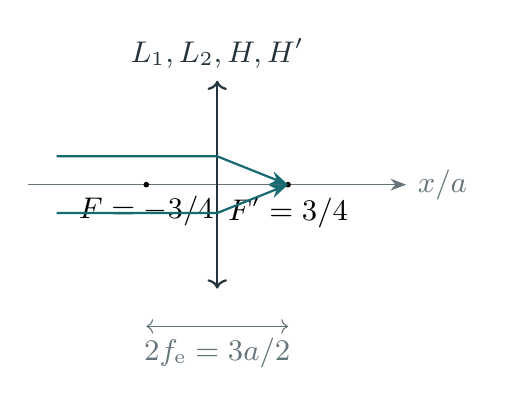
\begin{tikzpicture}[scale=1.2,transform shape]
\draw[axis] (-2,0)--(2,0) node[right] {$x/a$};\draw[object,<->] (0,-1.1)--(0,1.1) node[above] {$L_1,L_2,H,H'$};
\fill (-.75,0) circle(.03) node[below] {$F=-3/4$};\fill (.75,0) circle(.03) node[below] {$F'=3/4$};
\draw[motion] (-1.7,.3)--(0,.3)--(.75,0);\draw[motion] (-1.7,-.3)--(0,-.3)--(.75,0);
\draw[axis,<->] (-.75,-1.5)--(.75,-1.5) node[midway,below] {$2f_{\rm e}=3a/2$};\end{tikzpicture}
\figcaption{解图光试.3V2\quad 贴合极限的两主面重合于透镜平面}
\end{minipage}\end{center}
\Needspace{37\baselineskip}
\item \textbf{题设与求解。}间距取$d=f_1+f_2$，求平行光入射时的出射方向和横向尺度。

此时组合矩阵为
\[
M=\begin{pmatrix}-f_2/f_1&f_1+f_2\\0&-f_1/f_2\end{pmatrix}.
\]
出射斜率为$\vartheta_{\rm out}=-(f_1/f_2)\vartheta_{\rm in}$，与入射高度无关，所以同一方向的平行光仍为平行光，角倍率为$-f_1/f_2$。轴向入射时$y_{\rm out}=-(f_2/f_1)y_{\rm in}$。图V3取$f_1=3a,f_2=a,d=4a$，光束宽度成为三分之一，角倍率为$-3$。矩阵$C=0$给出无焦系统，焦点移至无穷远，此时用上述角度和光束尺度描述成像作用。
\begin{center}\begin{minipage}{.98\linewidth}\centering
\begin{tikzpicture}[scale=0.85,transform shape]
\draw[axis] (0,0)--(7.2,0);\draw[axis] (0,0)--(0,2.9000000000000004);
\draw[thin,color=muted] (0.7241379,0)--(0.7241379,-.07);\node[below] at (0.7241379,-.09) {$0$};
\draw[thin,color=muted] (5.5517241,0)--(5.5517241,-.07);\node[below] at (5.5517241,-.09) {$4$};
\draw[thin,color=muted] (0,1.3500000)--(-.07,1.3500000);\node[left] at (-.09,1.3500000) {$0$};
\node[below] at (3.5,-.64) {$x/a$};\node[above right] at (0,2.95) {$y/a$};
\draw[guide] (0,1.3500000)--(7.0,1.3500000);\draw[object,<->] (0.7241379,.1)--(0.7241379,2.6000000) node[above] {$L_1$};\draw[object,<->] (5.5517241,.1)--(5.5517241,2.6000000) node[above] {$L_2$};\draw[traj] plot coordinates {(0.2413793,2.1214286) (0.7241379,2.1214286) (5.5517241,1.0928571) (6.7586207,1.0928571)};
\draw[force] plot coordinates {(0.2413793,0.5785714) (0.7241379,0.5785714) (5.5517241,1.6071429) (6.7586207,1.6071429)};
\node[above] at (3.5,3.7) {$d=f_1+f_2$：轴向平行入射仍平行出射};\end{tikzpicture}
\figcaption{解图光试.3V3\quad 无焦组合：束宽三分之一，角倍率负3}
\end{minipage}\end{center}
\Needspace{37\baselineskip}
\item \textbf{题设与求解。}用平行入射的实际光线求惠更斯目镜的后焦点，并与主面求法联系。

平行光以高度$y$到达$L_1$，经第一镜后的斜率为$-y/(3a)$。传播$2a$至第二镜，高度变为$y_2=y-2y/3=y/3$。第二镜再次折射后
\[
\vartheta_2=-\frac{y}{3a}-\frac{y/3}{a}=-\frac{2y}{3a}=-\frac{y}{f_{\rm e}}.
\]
因此到轴上交点的距离为$-(y/3)/\vartheta_2=a/2$，后焦点绝对坐标为$2a+a/2=5a/2$。图V4画出正负两个入射高度的会聚光线；从$H'$到该点为$3a/2$，从第二镜到该点为$a/2$。
\begin{center}\begin{minipage}{.98\linewidth}\centering
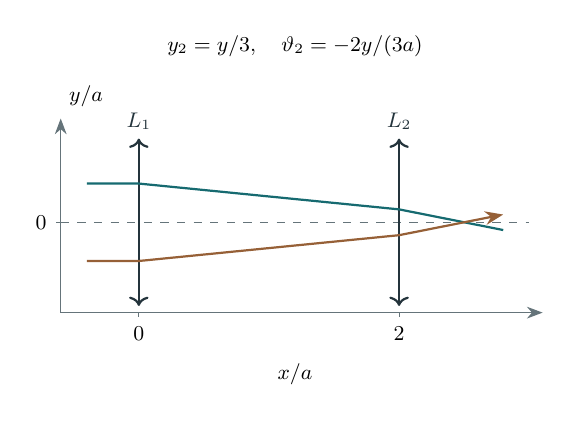
\begin{tikzpicture}[scale=0.85,transform shape]
\draw[axis] (0,0)--(7.2,0);\draw[axis] (0,0)--(0,2.9000000000000004);
\draw[thin,color=muted] (1.1666667,0)--(1.1666667,-.07);\node[below] at (1.1666667,-.09) {$0$};
\draw[thin,color=muted] (5.0555556,0)--(5.0555556,-.07);\node[below] at (5.0555556,-.09) {$2$};
\draw[thin,color=muted] (0,1.3500000)--(-.07,1.3500000);\node[left] at (-.09,1.3500000) {$0$};
\node[below] at (3.5,-.64) {$x/a$};\node[above right] at (0,2.95) {$y/a$};
\draw[guide] (0,1.3500000)--(7.0,1.3500000);\draw[object,<->] (1.1666667,.1)--(1.1666667,2.6000000) node[above] {$L_1$};\draw[object,<->] (5.0555556,.1)--(5.0555556,2.6000000) node[above] {$L_2$};\draw[traj] plot coordinates {(0.3888889,1.9285714) (1.1666667,1.9285714) (5.0555556,1.5428571) (6.6111111,1.2342857)};
\draw[force] plot coordinates {(0.3888889,0.7714286) (1.1666667,0.7714286) (5.0555556,1.1571429) (6.6111111,1.4657143)};
\node[above] at (3.5,3.7) {$y_2=y/3,\quad\vartheta_2=-2y/(3a)$};\end{tikzpicture}
\figcaption{解图光试.3V4\quad 实际后焦距为a除以2，有效焦距从像方主点量起}
\end{minipage}\end{center}
\Needspace{37\baselineskip}
\item \textbf{题设与求解。}从实际物像关系说明两目镜作普通放大镜的差别。惠更斯物体在$x=-u$，$u>0$；冉斯登取物点略在前焦面右方，$x=-a/4+\epsilon$，$0<\epsilon<a/4$。

惠更斯由物面至第二镜后的矩阵给$B=u/3+2a$、$D=-1-2u/(3a)$。最后像距第二镜为
\[
v=-B/D=\frac{u/3+2a}{1+2u/(3a)}>0,\quad
m=1/D=-\frac1{1+2u/(3a)}.
\]
图V5的这个前置实物形成倒立、缩小的实像。冉斯登则以主面量取物距$s=3a/4-\epsilon=f_{\rm e}-\epsilon$，薄透镜公式给
\[
s'=-\frac{f_{\rm e}(f_{\rm e}-\epsilon)}{\epsilon},\quad
m=-s'/s=\frac{f_{\rm e}}{\epsilon}>1.
\]
像距为负、倍率为正，形成正立放大虚像。取$\epsilon=a/20$，倍率为15，虚像绝对坐标为$a/6-21a/2=-31a/3$。
\begin{center}\begin{minipage}{.98\linewidth}\centering
\begin{tikzpicture}[scale=0.8,transform shape]
\draw[axis] (0,0)--(6.2,0);\draw[axis] (0,0)--(0,3.4000000000000004);
\draw[thin,color=muted] (0.0000000,0)--(0.0000000,-.07);\node[below] at (0.0000000,-.09) {$.02$};
\draw[thin,color=muted] (2.9696970,0)--(2.9696970,-.07);\node[below] at (2.9696970,-.09) {$1$};
\draw[thin,color=muted] (6.0000000,0)--(6.0000000,-.07);\node[below] at (6.0000000,-.09) {$2$};
\draw[thin,color=muted] (0,0.0000000)--(-.07,0.0000000);\node[left] at (-.09,0.0000000) {$1$};
\draw[thin,color=muted] (0,1.4545455)--(-.07,1.4545455);\node[left] at (-.09,1.4545455) {$1.5$};
\draw[thin,color=muted] (0,2.9090909)--(-.07,2.9090909);\node[left] at (-.09,2.9090909) {$2$};
\node[below] at (3.0,-.64) {$u/a$};\node[above right] at (0,3.45) {距第二镜的实像距离$/a$};
\draw[traj] plot coordinates {(0.0000000,2.8516746) (0.0250000,2.8284282) (0.0500000,2.8054315) (0.0750000,2.7826803) (0.1000000,2.7601709) (0.1250000,2.7378994) (0.1500000,2.7158620) (0.1750000,2.6940551) (0.2000000,2.6724751) (0.2250000,2.6511184) (0.2500000,2.6299816) (0.2750000,2.6090613) (0.3000000,2.5883542) (0.3250000,2.5678571) (0.3500000,2.5475668) (0.3750000,2.5274801) (0.4000000,2.5075941) (0.4250000,2.4879057) (0.4500000,2.4684120) (0.4750000,2.4491102) (0.5000000,2.4299973) (0.5250000,2.4110707) (0.5500000,2.3923276) (0.5750000,2.3737654) (0.6000000,2.3553815) (0.6250000,2.3371733) (0.6500000,2.3191383) (0.6750000,2.3012741) (0.7000000,2.2835782) (0.7250000,2.2660483) (0.7500000,2.2486820) (0.7750000,2.2314771) (0.8000000,2.2144313) (0.8250000,2.1975424) (0.8500000,2.1808084) (0.8750000,2.1642269) (0.9000000,2.1477961) (0.9250000,2.1315137) (0.9500000,2.1153779) (0.9750000,2.0993867) (1.0000000,2.0835381) (1.0250000,2.0678302) (1.0500000,2.0522612) (1.0750000,2.0368292) (1.1000000,2.0215324) (1.1250000,2.0063690) (1.1500000,1.9913374) (1.1750000,1.9764358) (1.2000000,1.9616626) (1.2250000,1.9470160) (1.2500000,1.9324944) (1.2750000,1.9180963) (1.3000000,1.9038201) (1.3250000,1.8896643) (1.3500000,1.8756273) (1.3750000,1.8617076) (1.4000000,1.8479039) (1.4250000,1.8342145) (1.4500000,1.8206382) (1.4750000,1.8071735) (1.5000000,1.7938191) (1.5250000,1.7805736) (1.5500000,1.7674356) (1.5750000,1.7544039) (1.6000000,1.7414773) (1.6250000,1.7286543) (1.6500000,1.7159339) (1.6750000,1.7033147) (1.7000000,1.6907955) (1.7250000,1.6783752) (1.7500000,1.6660527) (1.7750000,1.6538266) (1.8000000,1.6416961) (1.8250000,1.6296598) (1.8500000,1.6177167) (1.8750000,1.6058658) (1.9000000,1.5941059) (1.9250000,1.5824361) (1.9500000,1.5708553) (1.9750000,1.5593625) (2.0000000,1.5479566) (2.0250000,1.5366368) (2.0500000,1.5254020) (2.0750000,1.5142513) (2.1000000,1.5031837) (2.1250000,1.4921983) (2.1500000,1.4812942) (2.1750000,1.4704705) (2.2000000,1.4597264) (2.2250000,1.4490609) (2.2500000,1.4384731) (2.2750000,1.4279623) (2.3000000,1.4175276) (2.3250000,1.4071682) (2.3500000,1.3968832) (2.3750000,1.3866719) (2.4000000,1.3765335) (2.4250000,1.3664672) (2.4500000,1.3564722) (2.4750000,1.3465477) (2.5000000,1.3366932) (2.5250000,1.3269077) (2.5500000,1.3171905) (2.5750000,1.3075411) (2.6000000,1.2979586) (2.6250000,1.2884423) (2.6500000,1.2789916) (2.6750000,1.2696058) (2.7000000,1.2602843) (2.7250000,1.2510263) (2.7500000,1.2418313) (2.7750000,1.2326985) (2.8000000,1.2236274) (2.8250000,1.2146174) (2.8500000,1.2056677) (2.8750000,1.1967779) (2.9000000,1.1879473) (2.9250000,1.1791753) (2.9500000,1.1704614) (2.9750000,1.1618049) (3.0000000,1.1532054) (3.0250000,1.1446621) (3.0500000,1.1361747) (3.0750000,1.1277426) (3.1000000,1.1193651) (3.1250000,1.1110418) (3.1500000,1.1027722) (3.1750000,1.0945557) (3.2000000,1.0863919) (3.2250000,1.0782801) (3.2500000,1.0702200) (3.2750000,1.0622111) (3.3000000,1.0542528) (3.3250000,1.0463446) (3.3500000,1.0384862) (3.3750000,1.0306770) (3.4000000,1.0229165) (3.4250000,1.0152044) (3.4500000,1.0075401) (3.4750000,0.9999233) (3.5000000,0.9923534) (3.5250000,0.9848301) (3.5500000,0.9773529) (3.5750000,0.9699215) (3.6000000,0.9625352) (3.6250000,0.9551939) (3.6500000,0.9478970) (3.6750000,0.9406442) (3.7000000,0.9334350) (3.7250000,0.9262691) (3.7500000,0.9191461) (3.7750000,0.9120656) (3.8000000,0.9050272) (3.8250000,0.8980305) (3.8500000,0.8910752) (3.8750000,0.8841609) (3.9000000,0.8772873) (3.9250000,0.8704539) (3.9500000,0.8636605) (3.9750000,0.8569067) (4.0000000,0.8501921) (4.0250000,0.8435164) (4.0500000,0.8368792) (4.0750000,0.8302803) (4.1000000,0.8237193) (4.1250000,0.8171958) (4.1500000,0.8107096) (4.1750000,0.8042604) (4.2000000,0.7978477) (4.2250000,0.7914714) (4.2500000,0.7851310) (4.2750000,0.7788264) (4.3000000,0.7725571) (4.3250000,0.7663230) (4.3500000,0.7601237) (4.3750000,0.7539588) (4.4000000,0.7478282) (4.4250000,0.7417316) (4.4500000,0.7356685) (4.4750000,0.7296389) (4.5000000,0.7236424) (4.5250000,0.7176787) (4.5500000,0.7117476) (4.5750000,0.7058488) (4.6000000,0.6999820) (4.6250000,0.6941471) (4.6500000,0.6883436) (4.6750000,0.6825714) (4.7000000,0.6768302) (4.7250000,0.6711197) (4.7500000,0.6654398) (4.7750000,0.6597902) (4.8000000,0.6541706) (4.8250000,0.6485808) (4.8500000,0.6430205) (4.8750000,0.6374896) (4.9000000,0.6319877) (4.9250000,0.6265147) (4.9500000,0.6210704) (4.9750000,0.6156544) (5.0000000,0.6102667) (5.0250000,0.6049069) (5.0500000,0.5995749) (5.0750000,0.5942704) (5.1000000,0.5889933) (5.1250000,0.5837432) (5.1500000,0.5785201) (5.1750000,0.5733237) (5.2000000,0.5681537) (5.2250000,0.5630101) (5.2500000,0.5578925) (5.2750000,0.5528009) (5.3000000,0.5477349) (5.3250000,0.5426945) (5.3500000,0.5376793) (5.3750000,0.5326893) (5.4000000,0.5277242) (5.4250000,0.5227839) (5.4500000,0.5178681) (5.4750000,0.5129768) (5.5000000,0.5081096) (5.5250000,0.5032664) (5.5500000,0.4984471) (5.5750000,0.4936514) (5.6000000,0.4888793) (5.6250000,0.4841305) (5.6500000,0.4794048) (5.6750000,0.4747021) (5.7000000,0.4700222) (5.7250000,0.4653649) (5.7500000,0.4607302) (5.7750000,0.4561178) (5.8000000,0.4515275) (5.8250000,0.4469592) (5.8500000,0.4424128) (5.8750000,0.4378881) (5.9000000,0.4333849) (5.9250000,0.4289031) (5.9500000,0.4244425) (5.9750000,0.4200030) (6.0000000,0.4155844)};
\draw[traj] (.1,-1.08)--(.7,-1.08);\node[right] at (.85,-1.08) {惠更斯：$v/a>0$};\begin{scope}[yshift=-7.5cm]\draw[axis] (0,0)--(6.2,0);\draw[axis] (0,0)--(0,3.4000000000000004);
\draw[thin,color=muted] (0.3750000,0)--(0.3750000,-.07);\node[below] at (0.3750000,-.09) {$.05$};
\draw[thin,color=muted] (2.2500000,0)--(2.2500000,-.07);\node[below] at (2.2500000,-.09) {$.1$};
\draw[thin,color=muted] (6.0000000,0)--(6.0000000,-.07);\node[below] at (6.0000000,-.09) {$.2$};
\draw[thin,color=muted] (0,0.4571429)--(-.07,0.4571429);\node[left] at (-.09,0.4571429) {$-12$};
\draw[thin,color=muted] (0,1.8285714)--(-.07,1.8285714);\node[left] at (-.09,1.8285714) {$-6$};
\draw[thin,color=muted] (0,3.2000000)--(-.07,3.2000000);\node[left] at (-.09,3.2000000) {$0$};
\node[below] at (3.0,-.64) {$\epsilon/a$};\node[above right] at (0,3.45) {从像方主点量取的虚像距离$/a$};
\draw[traj] plot coordinates {(0.0000000,0.1571429) (0.0250000,0.2098361) (0.0500000,0.2608295) (0.0750000,0.3102041) (0.1000000,0.3580357) (0.1250000,0.4043956) (0.1500000,0.4493506) (0.1750000,0.4929638) (0.2000000,0.5352941) (0.2250000,0.5763975) (0.2500000,0.6163265) (0.2750000,0.6551308) (0.3000000,0.6928571) (0.3250000,0.7295499) (0.3500000,0.7652510) (0.3750000,0.8000000) (0.4000000,0.8338346) (0.4250000,0.8667904) (0.4500000,0.8989011) (0.4750000,0.9301989) (0.5000000,0.9607143) (0.5250000,0.9904762) (0.5500000,1.0195122) (0.5750000,1.0478485) (0.6000000,1.0755102) (0.6250000,1.1025210) (0.6500000,1.1289037) (0.6750000,1.1546798) (0.7000000,1.1798701) (0.7250000,1.2044944) (0.7500000,1.2285714) (0.7750000,1.2521193) (0.8000000,1.2751553) (0.8250000,1.2976959) (0.8500000,1.3197568) (0.8750000,1.3413534) (0.9000000,1.3625000) (0.9250000,1.3832106) (0.9500000,1.4034985) (0.9750000,1.4233766) (1.0000000,1.4428571) (1.0250000,1.4619519) (1.0500000,1.4806723) (1.0750000,1.4990291) (1.1000000,1.5170330) (1.1250000,1.5346939) (1.1500000,1.5520216) (1.1750000,1.5690254) (1.2000000,1.5857143) (1.2250000,1.6020970) (1.2500000,1.6181818) (1.2750000,1.6339768) (1.3000000,1.6494898) (1.3250000,1.6647282) (1.3500000,1.6796992) (1.3750000,1.6944099) (1.4000000,1.7088670) (1.4250000,1.7230769) (1.4500000,1.7370460) (1.4750000,1.7507803) (1.5000000,1.7642857) (1.5250000,1.7775679) (1.5500000,1.7906323) (1.5750000,1.8034843) (1.6000000,1.8161290) (1.6250000,1.8285714) (1.6500000,1.8408163) (1.6750000,1.8528684) (1.7000000,1.8647321) (1.7250000,1.8764120) (1.7500000,1.8879121) (1.7750000,1.8992366) (1.8000000,1.9103896) (1.8250000,1.9213749) (1.8500000,1.9321962) (1.8750000,1.9428571) (1.9000000,1.9533613) (1.9250000,1.9637122) (1.9500000,1.9739130) (1.9750000,1.9839671) (2.0000000,1.9938776) (2.0250000,2.0036474) (2.0500000,2.0132797) (2.0750000,2.0227772) (2.1000000,2.0321429) (2.1250000,2.0413793) (2.1500000,2.0504892) (2.1750000,2.0594752) (2.2000000,2.0683398) (2.2250000,2.0770853) (2.2500000,2.0857143) (2.2750000,2.0942289) (2.3000000,2.1026316) (2.3250000,2.1109244) (2.3500000,2.1191095) (2.3750000,2.1271889) (2.4000000,2.1351648) (2.4250000,2.1430391) (2.4500000,2.1508137) (2.4750000,2.1584906) (2.5000000,2.1660714) (2.5250000,2.1735581) (2.5500000,2.1809524) (2.5750000,2.1882559) (2.6000000,2.1954704) (2.6250000,2.2025974) (2.6500000,2.2096386) (2.6750000,2.2165954) (2.7000000,2.2234694) (2.7250000,2.2302620) (2.7500000,2.2369748) (2.7750000,2.2436090) (2.8000000,2.2501661) (2.8250000,2.2566474) (2.8500000,2.2630542) (2.8750000,2.2693878) (2.9000000,2.2756494) (2.9250000,2.2818402) (2.9500000,2.2879615) (2.9750000,2.2940144) (3.0000000,2.3000000) (3.0250000,2.3059195) (3.0500000,2.3117739) (3.0750000,2.3175644) (3.1000000,2.3232919) (3.1250000,2.3289575) (3.1500000,2.3345622) (3.1750000,2.3401070) (3.2000000,2.3455927) (3.2250000,2.3510204) (3.2500000,2.3563910) (3.2750000,2.3617053) (3.3000000,2.3669643) (3.3250000,2.3721688) (3.3500000,2.3773196) (3.3750000,2.3824176) (3.4000000,2.3874636) (3.4250000,2.3924583) (3.4500000,2.3974026) (3.4750000,2.4022972) (3.5000000,2.4071429) (3.5250000,2.4119403) (3.5500000,2.4166902) (3.5750000,2.4213934) (3.6000000,2.4260504) (3.6250000,2.4306620) (3.6500000,2.4352288) (3.6750000,2.4397516) (3.7000000,2.4442308) (3.7250000,2.4486671) (3.7500000,2.4530612) (3.7750000,2.4574137) (3.8000000,2.4617251) (3.8250000,2.4659960) (3.8500000,2.4702270) (3.8750000,2.4744186) (3.9000000,2.4785714) (3.9250000,2.4826860) (3.9500000,2.4867628) (3.9750000,2.4908023) (4.0000000,2.4948052) (4.0250000,2.4987718) (4.0500000,2.5027027) (4.0750000,2.5065983) (4.1000000,2.5104592) (4.1250000,2.5142857) (4.1500000,2.5180784) (4.1750000,2.5218376) (4.2000000,2.5255639) (4.2250000,2.5292576) (4.2500000,2.5329193) (4.2750000,2.5365492) (4.3000000,2.5401478) (4.3250000,2.5437155) (4.3500000,2.5472527) (4.3750000,2.5507599) (4.4000000,2.5542373) (4.4250000,2.5576854) (4.4500000,2.5611044) (4.4750000,2.5644949) (4.5000000,2.5678571) (4.5250000,2.5711915) (4.5500000,2.5744982) (4.5750000,2.5777778) (4.6000000,2.5810304) (4.6250000,2.5842566) (4.6500000,2.5874564) (4.6750000,2.5906304) (4.7000000,2.5937788) (4.7250000,2.5969019) (4.7500000,2.6000000) (4.7750000,2.6030734) (4.8000000,2.6061224) (4.8250000,2.6091474) (4.8500000,2.6121485) (4.8750000,2.6151261) (4.9000000,2.6180804) (4.9250000,2.6210117) (4.9500000,2.6239203) (4.9750000,2.6268064) (5.0000000,2.6296703) (5.0250000,2.6325123) (5.0500000,2.6353326) (5.0750000,2.6381315) (5.1000000,2.6409091) (5.1250000,2.6436658) (5.1500000,2.6464017) (5.1750000,2.6491172) (5.2000000,2.6518124) (5.2250000,2.6544875) (5.2500000,2.6571429) (5.2750000,2.6597786) (5.3000000,2.6623950) (5.3250000,2.6649922) (5.3500000,2.6675704) (5.3750000,2.6701299) (5.4000000,2.6726708) (5.4250000,2.6751934) (5.4500000,2.6776978) (5.4750000,2.6801843) (5.5000000,2.6826531) (5.5250000,2.6851042) (5.5500000,2.6875380) (5.5750000,2.6899546) (5.6000000,2.6923541) (5.6250000,2.6947368) (5.6500000,2.6971029) (5.6750000,2.6994525) (5.7000000,2.7017857) (5.7250000,2.7041028) (5.7500000,2.7064039) (5.7750000,2.7086892) (5.8000000,2.7109589) (5.8250000,2.7132131) (5.8500000,2.7154519) (5.8750000,2.7176755) (5.9000000,2.7198842) (5.9250000,2.7220779) (5.9500000,2.7242570) (5.9750000,2.7264214) (6.0000000,2.7285714)};
\draw[traj] (.1,-1.08)--(.7,-1.08);\node[right] at (.85,-1.08) {冉斯登：$s^\prime/a<0$};\end{scope}\end{tikzpicture}
\figcaption{解图光试.3V5\quad 前置实物的实像与前焦面内物体的放大虚像分别由有向像距描述}
\end{minipage}\end{center}
\Needspace{37\baselineskip}
\item \textbf{题设与求解。}冉斯登两镜焦距均为$a=4\,\mathrm{cm}$，间距$2a/3$。物在整组前焦面、眼观察平行出射光，以明视距离$25\,\mathrm{cm}$定义角放大率，求其数值。

有效焦距为$3a/4=3\,\mathrm{cm}$，前焦面在第一镜前$a/4=1\,\mathrm{cm}$。高为$y$的物点在前焦面出射为平行光，其倾角大小为$|y|/f_{\rm e}$；同一物体在明视距离裸眼张角约为$|y|/25\,\mathrm{cm}$。故
\[
G=\frac{25\,\mathrm{cm}}{3\,\mathrm{cm}}=\frac{25}{3}\simeq8.33.
\]
图V6用两条从同一离轴物点发出的光线表示平行出射；光线高度可不同，出射斜率相同，角放大率取其方向与裸眼张角之比。
\begin{center}\begin{minipage}{.98\linewidth}\centering
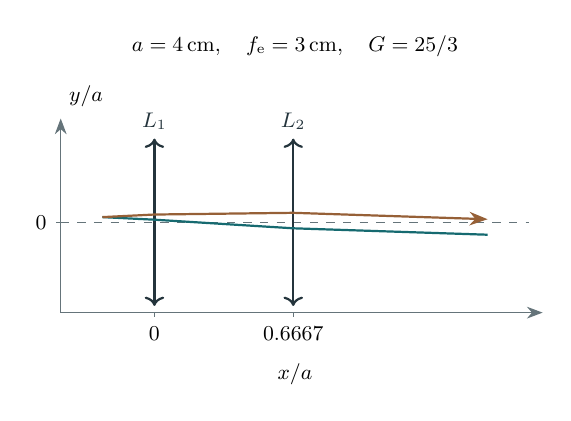
\begin{tikzpicture}[scale=0.85,transform shape]
\draw[axis] (0,0)--(7.2,0);\draw[axis] (0,0)--(0,2.9000000000000004);
\draw[thin,color=muted] (1.4000000,0)--(1.4000000,-.07);\node[below] at (1.4000000,-.09) {$0$};
\draw[thin,color=muted] (3.4740741,0)--(3.4740741,-.07);\node[below] at (3.4740741,-.09) {$0.6667$};
\draw[thin,color=muted] (0,1.3500000)--(-.07,1.3500000);\node[left] at (-.09,1.3500000) {$0$};
\node[below] at (3.5,-.64) {$x/a$};\node[above right] at (0,2.95) {$y/a$};
\draw[guide] (0,1.3500000)--(7.0,1.3500000);\draw[object,<->] (1.4000000,.1)--(1.4000000,2.6000000) node[above] {$L_1$};\draw[object,<->] (3.4740741,.1)--(3.4740741,2.6000000) node[above] {$L_2$};\draw[traj] plot coordinates {(0.6222222,1.4271429) (1.4000000,1.3885714) (3.4740741,1.2600000) (6.3777778,1.1640000)};
\draw[force] plot coordinates {(0.6222222,1.4271429) (1.4000000,1.4657143) (3.4740741,1.4914286) (6.3777778,1.3954286)};
\node[above] at (3.5,3.7) {$a=4\,\mathrm{cm},\quad f_{\rm e}=3\,\mathrm{cm},\quad G=25/3$};\end{tikzpicture}
\figcaption{解图光试.3V6\quad 同一前焦面物点发出的两条光线平行出射}
\end{minipage}\end{center}
\Needspace{37\baselineskip}
\item \textbf{题设与求解。}假设两镜具有相同的相对色散，写$f_i(\lambda)=k(\lambda)f_{i0}$，镜间距$d$固定，设计波长处$k=1$。比较两种组合的等效光焦度对$k$的一阶变化。

由通式
\[
\Phi(k)=\frac{1/f_{10}+1/f_{20}}{k}-\frac{d}{f_{10}f_{20}k^2},\quad
\Phi'(1)=-\frac{f_{10}+f_{20}-2d}{f_{10}f_{20}}.
\]
惠更斯满足$2d=f_{10}+f_{20}=4a$，故一阶变化为零。令$k=1+\eta$，有$a\Phi=2/3-2\eta^2/3+O(\eta^3)$。冉斯登则$a\Phi=4/3-2\eta/3+O(\eta^3)$，保留一阶色散。图V7比较这两个光焦度的相对变化。这里求的是组合光焦度的色散，主面位置还随$f_1,f_2$改变，可由主点公式分别计算。
\begin{center}\begin{minipage}{.98\linewidth}\centering
\begin{tikzpicture}[scale=0.72,transform shape]
\draw[axis] (0,0)--(6.2,0);\draw[axis] (0,0)--(0,3.4000000000000004);
\draw[thin,color=muted] (0.0000000,0)--(0.0000000,-.07);\node[below] at (0.0000000,-.09) {$.96$};
\draw[thin,color=muted] (3.0000000,0)--(3.0000000,-.07);\node[below] at (3.0000000,-.09) {$1$};
\draw[thin,color=muted] (6.0000000,0)--(6.0000000,-.07);\node[below] at (6.0000000,-.09) {$1.04$};
\draw[thin,color=muted] (0,0.5333333)--(-.07,0.5333333);\node[left] at (-.09,0.5333333) {$.98$};
\draw[thin,color=muted] (0,1.6000000)--(-.07,1.6000000);\node[left] at (-.09,1.6000000) {$1$};
\draw[thin,color=muted] (0,2.6666667)--(-.07,2.6666667);\node[left] at (-.09,2.6666667) {$1.02$};
\node[below] at (3.0,-.64) {相对焦距因子$k$};\node[above right] at (0,3.45) {$\Phi(k)/\Phi(1)$};
\draw[traj] plot coordinates {(0.0000000,1.5074074) (0.0250000,1.5090074) (0.0500000,1.5105923) (0.0750000,1.5121623) (0.1000000,1.5137172) (0.1250000,1.5152572) (0.1500000,1.5167823) (0.1750000,1.5182925) (0.2000000,1.5197878) (0.2250000,1.5212683) (0.2500000,1.5227340) (0.2750000,1.5241849) (0.3000000,1.5256211) (0.3250000,1.5270426) (0.3500000,1.5284494) (0.3750000,1.5298415) (0.4000000,1.5312190) (0.4250000,1.5325819) (0.4500000,1.5339303) (0.4750000,1.5352641) (0.5000000,1.5365834) (0.5250000,1.5378883) (0.5500000,1.5391786) (0.5750000,1.5404546) (0.6000000,1.5417162) (0.6250000,1.5429634) (0.6500000,1.5441963) (0.6750000,1.5454148) (0.7000000,1.5466191) (0.7250000,1.5478092) (0.7500000,1.5489850) (0.7750000,1.5501467) (0.8000000,1.5512941) (0.8250000,1.5524275) (0.8500000,1.5535467) (0.8750000,1.5546519) (0.9000000,1.5557430) (0.9250000,1.5568201) (0.9500000,1.5578832) (0.9750000,1.5589323) (1.0000000,1.5599675) (1.0250000,1.5609888) (1.0500000,1.5619962) (1.0750000,1.5629897) (1.1000000,1.5639694) (1.1250000,1.5649353) (1.1500000,1.5658875) (1.1750000,1.5668259) (1.2000000,1.5677506) (1.2250000,1.5686616) (1.2500000,1.5695590) (1.2750000,1.5704427) (1.3000000,1.5713128) (1.3250000,1.5721693) (1.3500000,1.5730123) (1.3750000,1.5738417) (1.4000000,1.5746577) (1.4250000,1.5754601) (1.4500000,1.5762492) (1.4750000,1.5770248) (1.5000000,1.5777870) (1.5250000,1.5785359) (1.5500000,1.5792714) (1.5750000,1.5799936) (1.6000000,1.5807026) (1.6250000,1.5813983) (1.6500000,1.5820807) (1.6750000,1.5827500) (1.7000000,1.5834060) (1.7250000,1.5840489) (1.7500000,1.5846787) (1.7750000,1.5852954) (1.8000000,1.5858990) (1.8250000,1.5864896) (1.8500000,1.5870672) (1.8750000,1.5876317) (1.9000000,1.5881833) (1.9250000,1.5887220) (1.9500000,1.5892477) (1.9750000,1.5897606) (2.0000000,1.5902605) (2.0250000,1.5907477) (2.0500000,1.5912220) (2.0750000,1.5916835) (2.1000000,1.5921323) (2.1250000,1.5925683) (2.1500000,1.5929917) (2.1750000,1.5934023) (2.2000000,1.5938003) (2.2250000,1.5941856) (2.2500000,1.5945584) (2.2750000,1.5949185) (2.3000000,1.5952661) (2.3250000,1.5956012) (2.3500000,1.5959237) (2.3750000,1.5962338) (2.4000000,1.5965314) (2.4250000,1.5968166) (2.4500000,1.5970893) (2.4750000,1.5973497) (2.5000000,1.5975977) (2.5250000,1.5978334) (2.5500000,1.5980568) (2.5750000,1.5982678) (2.6000000,1.5984667) (2.6250000,1.5986532) (2.6500000,1.5988276) (2.6750000,1.5989898) (2.7000000,1.5991398) (2.7250000,1.5992777) (2.7500000,1.5994034) (2.7750000,1.5995171) (2.8000000,1.5996187) (2.8250000,1.5997083) (2.8500000,1.5997858) (2.8750000,1.5998514) (2.9000000,1.5999049) (2.9250000,1.5999466) (2.9500000,1.5999763) (2.9750000,1.5999941) (3.0000000,1.6000000) (3.0250000,1.5999941) (3.0500000,1.5999763) (3.0750000,1.5999468) (3.1000000,1.5999054) (3.1250000,1.5998523) (3.1500000,1.5997875) (3.1750000,1.5997110) (3.2000000,1.5996228) (3.2250000,1.5995229) (3.2500000,1.5994113) (3.2750000,1.5992882) (3.3000000,1.5991535) (3.3250000,1.5990071) (3.3500000,1.5988493) (3.3750000,1.5986799) (3.4000000,1.5984990) (3.4250000,1.5983067) (3.4500000,1.5981028) (3.4750000,1.5978876) (3.5000000,1.5976609) (3.5250000,1.5974229) (3.5500000,1.5971735) (3.5750000,1.5969127) (3.6000000,1.5966406) (3.6250000,1.5963573) (3.6500000,1.5960626) (3.6750000,1.5957567) (3.7000000,1.5954396) (3.7250000,1.5951113) (3.7500000,1.5947718) (3.7750000,1.5944211) (3.8000000,1.5940593) (3.8250000,1.5936863) (3.8500000,1.5933023) (3.8750000,1.5929072) (3.9000000,1.5925011) (3.9250000,1.5920839) (3.9500000,1.5916557) (3.9750000,1.5912165) (4.0000000,1.5907664) (4.0250000,1.5903053) (4.0500000,1.5898333) (4.0750000,1.5893504) (4.1000000,1.5888567) (4.1250000,1.5883521) (4.1500000,1.5878366) (4.1750000,1.5873104) (4.2000000,1.5867733) (4.2250000,1.5862255) (4.2500000,1.5856669) (4.2750000,1.5850977) (4.3000000,1.5845177) (4.3250000,1.5839270) (4.3500000,1.5833257) (4.3750000,1.5827137) (4.4000000,1.5820911) (4.4250000,1.5814580) (4.4500000,1.5808142) (4.4750000,1.5801599) (4.5000000,1.5794951) (4.5250000,1.5788197) (4.5500000,1.5781339) (4.5750000,1.5774376) (4.6000000,1.5767308) (4.6250000,1.5760136) (4.6500000,1.5752860) (4.6750000,1.5745481) (4.7000000,1.5737997) (4.7250000,1.5730410) (4.7500000,1.5722720) (4.7750000,1.5714927) (4.8000000,1.5707031) (4.8250000,1.5699033) (4.8500000,1.5690932) (4.8750000,1.5682729) (4.9000000,1.5674423) (4.9250000,1.5666016) (4.9500000,1.5657508) (4.9750000,1.5648898) (5.0000000,1.5640187) (5.0250000,1.5631375) (5.0500000,1.5622462) (5.0750000,1.5613448) (5.1000000,1.5604334) (5.1250000,1.5595120) (5.1500000,1.5585806) (5.1750000,1.5576392) (5.2000000,1.5566879) (5.2250000,1.5557266) (5.2500000,1.5547554) (5.2750000,1.5537743) (5.3000000,1.5527833) (5.3250000,1.5517825) (5.3500000,1.5507718) (5.3750000,1.5497513) (5.4000000,1.5487210) (5.4250000,1.5476810) (5.4500000,1.5466311) (5.4750000,1.5455716) (5.5000000,1.5445023) (5.5250000,1.5434233) (5.5500000,1.5423346) (5.5750000,1.5412362) (5.6000000,1.5401282) (5.6250000,1.5390106) (5.6500000,1.5378834) (5.6750000,1.5367466) (5.7000000,1.5356002) (5.7250000,1.5344443) (5.7500000,1.5332789) (5.7750000,1.5321039) (5.8000000,1.5309195) (5.8250000,1.5297256) (5.8500000,1.5285222) (5.8750000,1.5273094) (5.9000000,1.5260872) (5.9250000,1.5248556) (5.9500000,1.5236146) (5.9750000,1.5223642) (6.0000000,1.5211045)};
\draw[traj] (.1,-1.08)--(.7,-1.08);\node[right] at (.85,-1.08) {惠更斯};\draw[dashed,thick,color=warm] plot coordinates {(0.0000000,2.6648148) (0.0250000,2.6559731) (0.0500000,2.6471305) (0.0750000,2.6382872) (0.1000000,2.6294430) (0.1250000,2.6205980) (0.1500000,2.6117522) (0.1750000,2.6029056) (0.2000000,2.5940583) (0.2250000,2.5852101) (0.2500000,2.5763612) (0.2750000,2.5675116) (0.3000000,2.5586612) (0.3250000,2.5498100) (0.3500000,2.5409582) (0.3750000,2.5321056) (0.4000000,2.5232522) (0.4250000,2.5143982) (0.4500000,2.5055435) (0.4750000,2.4966881) (0.5000000,2.4878319) (0.5250000,2.4789752) (0.5500000,2.4701177) (0.5750000,2.4612596) (0.6000000,2.4524008) (0.6250000,2.4435414) (0.6500000,2.4346813) (0.6750000,2.4258206) (0.7000000,2.4169593) (0.7250000,2.4080973) (0.7500000,2.3992348) (0.7750000,2.3903716) (0.8000000,2.3815079) (0.8250000,2.3726435) (0.8500000,2.3637786) (0.8750000,2.3549131) (0.9000000,2.3460471) (0.9250000,2.3371805) (0.9500000,2.3283133) (0.9750000,2.3194456) (1.0000000,2.3105773) (1.0250000,2.3017086) (1.0500000,2.2928393) (1.0750000,2.2839695) (1.1000000,2.2750992) (1.1250000,2.2662284) (1.1500000,2.2573571) (1.1750000,2.2484853) (1.2000000,2.2396130) (1.2250000,2.2307403) (1.2500000,2.2218671) (1.2750000,2.2129934) (1.3000000,2.2041193) (1.3250000,2.1952448) (1.3500000,2.1863698) (1.3750000,2.1774944) (1.4000000,2.1686186) (1.4250000,2.1597423) (1.4500000,2.1508657) (1.4750000,2.1419886) (1.5000000,2.1331112) (1.5250000,2.1242334) (1.5500000,2.1153552) (1.5750000,2.1064766) (1.6000000,2.0975977) (1.6250000,2.0887184) (1.6500000,2.0798387) (1.6750000,2.0709587) (1.7000000,2.0620784) (1.7250000,2.0531977) (1.7500000,2.0443168) (1.7750000,2.0354355) (1.8000000,2.0265539) (1.8250000,2.0176719) (1.8500000,2.0087897) (1.8750000,1.9999072) (1.9000000,1.9910245) (1.9250000,1.9821414) (1.9500000,1.9732581) (1.9750000,1.9643745) (2.0000000,1.9554906) (2.0250000,1.9466065) (2.0500000,1.9377222) (2.0750000,1.9288376) (2.1000000,1.9199528) (2.1250000,1.9110678) (2.1500000,1.9021825) (2.1750000,1.8932970) (2.2000000,1.8844114) (2.2250000,1.8755255) (2.2500000,1.8666395) (2.2750000,1.8577532) (2.3000000,1.8488668) (2.3250000,1.8399802) (2.3500000,1.8310934) (2.3750000,1.8222065) (2.4000000,1.8133195) (2.4250000,1.8044322) (2.4500000,1.7955449) (2.4750000,1.7866574) (2.5000000,1.7777698) (2.5250000,1.7688820) (2.5500000,1.7599942) (2.5750000,1.7511062) (2.6000000,1.7422181) (2.6250000,1.7333300) (2.6500000,1.7244417) (2.6750000,1.7155534) (2.7000000,1.7066649) (2.7250000,1.6977765) (2.7500000,1.6888879) (2.7750000,1.6799993) (2.8000000,1.6711106) (2.8250000,1.6622219) (2.8500000,1.6533331) (2.8750000,1.6444443) (2.9000000,1.6355555) (2.9250000,1.6266666) (2.9500000,1.6177778) (2.9750000,1.6088889) (3.0000000,1.6000000) (3.0250000,1.5911111) (3.0500000,1.5822222) (3.0750000,1.5733334) (3.1000000,1.5644445) (3.1250000,1.5555557) (3.1500000,1.5466669) (3.1750000,1.5377781) (3.2000000,1.5288894) (3.2250000,1.5200007) (3.2500000,1.5111121) (3.2750000,1.5022235) (3.3000000,1.4933350) (3.3250000,1.4844466) (3.3500000,1.4755582) (3.3750000,1.4666700) (3.4000000,1.4577818) (3.4250000,1.4488937) (3.4500000,1.4400057) (3.4750000,1.4311178) (3.5000000,1.4222300) (3.5250000,1.4133424) (3.5500000,1.4044548) (3.5750000,1.3955674) (3.6000000,1.3866801) (3.6250000,1.3777930) (3.6500000,1.3689060) (3.6750000,1.3600191) (3.7000000,1.3511324) (3.7250000,1.3422459) (3.7500000,1.3333595) (3.7750000,1.3244733) (3.8000000,1.3155872) (3.8250000,1.3067014) (3.8500000,1.2978157) (3.8750000,1.2889303) (3.9000000,1.2800450) (3.9250000,1.2711599) (3.9500000,1.2622751) (3.9750000,1.2533904) (4.0000000,1.2445060) (4.0250000,1.2356218) (4.0500000,1.2267378) (4.0750000,1.2178541) (4.1000000,1.2089706) (4.1250000,1.2000874) (4.1500000,1.1912044) (4.1750000,1.1823216) (4.2000000,1.1734391) (4.2250000,1.1645569) (4.2500000,1.1556750) (4.2750000,1.1467933) (4.3000000,1.1379120) (4.3250000,1.1290309) (4.3500000,1.1201501) (4.3750000,1.1112696) (4.4000000,1.1023894) (4.4250000,1.0935095) (4.4500000,1.0846299) (4.4750000,1.0757506) (4.5000000,1.0668717) (4.5250000,1.0579931) (4.5500000,1.0491148) (4.5750000,1.0402369) (4.6000000,1.0313593) (4.6250000,1.0224821) (4.6500000,1.0136052) (4.6750000,1.0047287) (4.7000000,0.9958525) (4.7250000,0.9869767) (4.7500000,0.9781013) (4.7750000,0.9692262) (4.8000000,0.9603516) (4.8250000,0.9514773) (4.8500000,0.9426034) (4.8750000,0.9337299) (4.9000000,0.9248568) (4.9250000,0.9159842) (4.9500000,0.9071119) (4.9750000,0.8982401) (5.0000000,0.8893686) (5.0250000,0.8804976) (5.0500000,0.8716271) (5.0750000,0.8627570) (5.1000000,0.8538873) (5.1250000,0.8450180) (5.1500000,0.8361492) (5.1750000,0.8272809) (5.2000000,0.8184130) (5.2250000,0.8095456) (5.2500000,0.8006787) (5.2750000,0.7918122) (5.3000000,0.7829462) (5.3250000,0.7740807) (5.3500000,0.7652157) (5.3750000,0.7563512) (5.4000000,0.7474871) (5.4250000,0.7386236) (5.4500000,0.7297606) (5.4750000,0.7208981) (5.5000000,0.7120361) (5.5250000,0.7031746) (5.5500000,0.6943136) (5.5750000,0.6854532) (5.6000000,0.6765933) (5.6250000,0.6677340) (5.6500000,0.6588752) (5.6750000,0.6500169) (5.7000000,0.6411592) (5.7250000,0.6323020) (5.7500000,0.6234454) (5.7750000,0.6145894) (5.8000000,0.6057339) (5.8250000,0.5968791) (5.8500000,0.5880247) (5.8750000,0.5791710) (5.9000000,0.5703179) (5.9250000,0.5614653) (5.9500000,0.5526134) (5.9750000,0.5437620) (6.0000000,0.5349112)};
\draw[dashed,thick,color=warm] (.1,-1.51)--(.7,-1.51);\node[right] at (.85,-1.51) {冉斯登};\end{tikzpicture}
\figcaption{解图光试.3V7\quad 相同相对色散模型下，惠更斯组合光焦度的一阶变化为零}
\end{minipage}\end{center}
\Needspace{37\baselineskip}
\item \textbf{题设与求解。}将惠更斯组合反向使用，从焦距为$a$的一镜先入射，另一镜焦距为$3a$，间距仍为$2a$。以新的第一镜为零点、入射方向为正，求四个点并讨论普通放大镜用法。

有效焦距仍为$3a/2$，但主点变为
\[
x_H=\frac{f_{\rm e}d}{3a}=a,\quad
x_{H'}=2a-\frac{f_{\rm e}d}{a}=-a,
\]
因此$x_F=-a/2$、$x_{F'}=a/2$。图V8中前焦面移至整组之前，实物可放在其右侧附近作为普通放大镜使用。用互易关系也得到$x_H^{\rm rev}=d-x_{H'}$、$x_{H'}^{\rm rev}=d-x_H$、$x_F^{\rm rev}=d-x_{F'}$和$x_{F'}^{\rm rev}=d-x_F$，各自给同一坐标；镜片顺序决定哪一端为物方。
\begin{center}\begin{minipage}{.98\linewidth}\centering
\begin{tikzpicture}[scale=1.2,transform shape]
\draw[axis] (-1.7,0)--(2.8,0) node[right] {$x/a$};
\draw[object,<->] (0,-1)--(0,1) node[above] {$L_1:f_1=a$};\draw[object,<->] (2,-1)--(2,1) node[above] {$L_2:f_2=3a$};
\draw[guide] (-1,0)--(-1,-1.5) node[below] {$H':-1$};\draw[guide] (1,0)--(1,-1.5) node[below] {$H:1$};
\fill (-.5,0) circle(.03);\draw[guide] (-.5,0)--(-.5,1.8) node[above] {$F:-1/2$};
\fill (.5,0) circle(.03);\draw[guide] (.5,0)--(.5,1.8) node[above] {$F':1/2$};
\node[below] at (.5,-2.5) {先经过短焦镜，前焦点移至整组之前};\end{tikzpicture}
\figcaption{解图光试.3V8\quad 反转镜片次序后，仍有相同有效焦距而主面位置改变}
\end{minipage}\end{center}
\end{enumerate}

\Needspace{13\baselineskip}

\pdfbookmark[2]{第 4 题 切接透镜的干涉条纹与有限重叠区}{q4}

\section*{第 4 题\quad 切接透镜的干涉条纹与有限重叠区}\label{q:4}


一焦距$f=20\,\mathrm{cm}$的薄凸透镜，从中央切去宽为$a$的条带，再把剩下两半向中间平移并粘接。两半的光心相距$a$，粘接后的总直径为$D=2.0\,\mathrm{cm}$。波长$\lambda=500\,\mathrm{nm}$的单色点光源$S$位于粘接体的中心轴线上，距透镜为$f$。透镜另一侧放置垂直中心轴的屏，测得条纹间距$\Delta y=0.20\,\mathrm{mm}$。
\begin{enumerate}
\item 求切去条带的宽度$a$。
\item 屏距透镜多远时，可见重叠区内的条纹数最多？给出中央纵截面内重叠宽度随屏距的变化。
\end{enumerate}
采用傍轴几何光学描述光束外缘，在两束的重叠区域计算干涉；忽略边缘衍射对外缘的模糊。


\begin{center}\begin{minipage}{.98\linewidth}\centering
\begin{tikzpicture}[scale=.7,transform shape]

\draw[object] (-1,1.9)..controls(-1.8,.5)and(-1.8,-.5)..(-1,-1.9);
\draw[object] (-1,1.9)..controls(-.2,.5)and(-.2,-.5)..(-1,-1.9);
\fill[white] (-1.9,-.4) rectangle (-.1,.4);
\draw[guide] (-1.65,.4)--(-.35,.4);\draw[guide] (-1.65,-.4)--(-.35,-.4);
\draw[axis,<->] (-2.2,-.4)--(-2.2,.4) node[midway,left] {$a$};
\draw[motion] (0,0)--(1,0);
\draw[object] (2,1.5)..controls(1.3,.3)and(1.3,-.3)..(2,-1.5);
\draw[object] (2,1.5)..controls(2.7,.3)and(2.7,-.3)..(2,-1.5);
\draw[object] (1.5,0)--(2.5,0);
\draw[axis,<->] (3,-1.5)--(3,1.5) node[midway,right,yshift=4pt] {$D$};
\begin{scope}[xshift=6cm]
\draw[axis] (-2.5,0)--(3.5,0);
\fill (-2,0) circle (1.8pt) node[above] {$S$};
\draw[object,<->] (0,-1.5)--(0,1.5);
\draw[object] (3,-2)--(3,2) node[above] {屏};
\draw[axis,<->] (-2,-2.3)--(0,-2.3) node[midway,below] {$f$};
\draw[axis,<->] (0,-2.9)--(3,-2.9) node[midway,below] {$z$};
\end{scope}

\end{tikzpicture}
\figcaption{图光试.4\quad 中央去条带后平移粘接，D指粘接后的总口径。}
\end{minipage}\end{center}

\Needspace{8\baselineskip}

\pdfbookmark[3]{题型定位}{q4-h0}

\subsection*{题型定位}

同一焦面点经偏轴半镜产生两束倾斜平面波，条纹间距由两波矢横分量之差确定，条纹覆盖范围由有限孔径决定。题目的优化量是重叠宽度，两部分通过同一个倾角相连。

\Needspace{8\baselineskip}

\pdfbookmark[3]{知识点}{q4-h1}

\subsection*{知识点}

前焦平面的点光源经过薄透镜后形成平行光，光束方向由光源相对镜片光轴的位置决定。两波矢之差给出相位梯度$2k\sin\theta$和间距$\lambda/(2\sin\theta)$。孔径的四条束边以各自斜率传播，两束的区间交集给出分段重叠。粘接后的直径$D$决定每半束截面的高度$D/2$。条纹间距数为宽度除以间距，亮纹条数由相位与整数中心位置确定。

\Needspace{8\baselineskip}

\pdfbookmark[3]{物理图像}{q4-h2}

\subsection*{物理图像}

解图光试.4A的上半束向下、下半束向上，阴影菱形是中央纵截面内的重叠。解图B画宽度随屏距的两段直线；在转折处两束中心重合，外侧束边接替内侧束边限制宽度。解图C用实际米和毫米为单位画四条极限光线，在2、4、6米处分别读出5、10、5毫米宽度。

\Needspace{8\baselineskip}

\pdfbookmark[3]{解题入口}{q4-h3}

\subsection*{解题入口}

先标上半镜光心在粘接中轴下方$a/2$，由薄透镜斜率关系求出负倾角；下半镜取相反方向。把两波矢横分量相减，得到间距并统一长度单位求$a$。再将上下半孔径的两个端点各平移$z\theta$，写出两个区间，以最小上端点减最大下端点求交集。

\Needspace{8\baselineskip}

\pdfbookmark[3]{标准解法}{q4-h4}

\subsection*{标准解法}


图光试.4中，上半镜向下平移$a/2$，其光轴在中心轴下方$a/2$；下半镜则相反。光源虽在粘接体中心轴上，却分别位于两片光轴的两侧，并处于各片前焦平面。
\begin{center}\begin{minipage}{.98\linewidth}\centering
\begin{tikzpicture}[scale=.7,transform shape]

\fill[accent!12] (0,0)--(4,1)--(8,0)--(4,-1)--cycle;
\draw[axis] (-3,0)--(9,0) node[right] {$z$};
\draw[object] (0,-2)--(0,2);
\draw[traj] (0,0)--(8,-2);\draw[traj] (0,2)--(8,0);
\draw[force] (0,-2)--(8,0);\draw[force] (0,0)--(8,2);
\draw[guide] (0,-.4)--(3,-.4);
\draw[guide] (0,.4)--(3,.4);
\node at (4,3.2) {上半镜轴$y=-a/2$；下半镜轴$y=+a/2$};
\fill (-1.6,0) circle (1.8pt) node[above] {$S$};
\draw[guide] (-1.6,0)--(0,-.4);\draw[guide] (-1.6,0)--(0,.4);
\draw[axis,<->] (-.8,-.4)--(-.8,.4) node[midway,left] {$a$};
\draw[object] (4,-2)--(4,2) node[above] {示例屏};
\draw[motion] (1,1.7)--(2,1.45) node[midway,above] {$-\theta$};
\draw[motion] (1,-1.7)--(2,-1.45) node[midway,below] {$+\theta$};
\node at (4,-3) {两束均为平面波，阴影为中央纵截面的重叠区};

\end{tikzpicture}
\figcaption{解图光试.4A\quad 光轴偏移决定向内倾角，光束外缘由半孔径分别平移。}
\end{minipage}\end{center}
解图光试.4A中，每半镜把来自$S$的球面波变为平面波。上半束向下、下半束向上，两束方向相对中心轴为$-\theta,+\theta$。以$y$轴向上、$z$轴向右表示传播。薄透镜的傍轴折射关系为$u_{\rm out}=u_{\rm in}-(y-y_c)/f$，轴上焦面点发出的光在透镜处有$u_{\rm in}=y/f$，所以$u_{\rm out}=y_c/f$，与落点$y$无关。两半镜的光心坐标$y_c=\mp a/2$直接给出两个相反斜率。傍轴下
\[
\theta\simeq\frac{a}{2f}.
\]
在屏上取纵向坐标$y$，两平面波的波矢纵分量差为$2k\sin\theta$，相位差随$y$变化为
\[
\Delta\varphi(y)=2k\,y\sin\theta+\varphi_0.
\]
相位差由$({\boldsymbol k}_2-{\boldsymbol k}_1)\cdot(0,y,z)$给出，两束的纵向分量同为$k\cos\theta$，传播距离项抵消，只余横向的$2ky\sin\theta$。相邻亮纹相位差$2\pi$，所以
\[
\Delta y=\frac{\lambda}{2\sin\theta}
\simeq\frac{\lambda f}{a}.
\]
代入同一单位：
\[
\boxed{a=\frac{\lambda f}{\Delta y}
=\frac{(5.00\times10^{-7})(0.200)}{2.00\times10^{-4}}
=5.00\times10^{-4}\,\mathrm m=0.50\,\mathrm{mm}}.
\]
两束来自同一点光源并通过同一镜体的两部分，具有固定相位关系。常量$\varphi_0$会平移条纹，但不改变间距。
\begin{center}\begin{minipage}{.98\linewidth}\centering
\begin{tikzpicture}[scale=.8,transform shape]

\draw[axis] (0,0)--(9,0) node[right] {$z$};
\draw[axis] (0,0)--(0,3) node[above] {$W$};
\draw[traj] (0,0)--(4,2)--(8,0);
\draw[guide] (4,0)--(4,2)--(0,2);
\node[left] at (0,2) {$D/2$};
\node[below] at (4,0) {$D/(4\theta)$};
\node[below] at (8,0) {$D/(2\theta)$};
\node[above left] at (2,1.2) {$2z\theta$};
\node[above right] at (6,1.2) {$D-2z\theta$};
\node at (4.5,3.8) {条纹间距固定，重叠宽度决定间距数};

\end{tikzpicture}
\figcaption{解图光试.4B\quad 两段束边限制交替，最宽处对应最佳屏距。}
\end{minipage}\end{center}
第（2）问沿两束的内、外侧各追踪一条极限光线，共得到四条束边。解图光试.4B在中央纵截面中取透镜平面为$z=0$，屏为$z>0$。上、下半孔径分别覆盖$[0,D/2]$与$[-D/2,0]$。到屏上，上束整体向下移$z\theta$、下束向上移$z\theta$，区间变成
\[
\mathcal B_+(z)=[-z\theta,D/2-z\theta],\qquad
\mathcal B_-(z)=[-D/2+z\theta,z\theta].
\]
重叠区是这两个区间的交集。取上端点的较小值、下端点的较大值，宽度为
\[
W=\max\{0,\min(D/2-z\theta,z\theta)-\max(-z\theta,-D/2+z\theta)\}.
\]
两个候选上端点在$z\theta=D/4$相等，下端点也在同一位置交换大小；整理得到
\[
\boxed{W(z)=
\begin{cases}
2z\theta,&0\le z\le D/(4\theta),\\
D-2z\theta,&D/(4\theta)\le z\le D/(2\theta),\\
0,&z\ge D/(2\theta).
\end{cases}}
\]
开始时相邻内束边向对方孔径区域移动，宽度增加；超过中点后，外束边逐渐限制重叠，宽度反而减小。条纹间距与$z$无关，所以条纹总数在$W$最大时最多：
\[
\boxed{z_{\rm best}=\frac D{4\theta}
\simeq\frac{Df}{2a}
=\frac{0.0200\times0.200}{2\times0.000500}
=4.0\,\mathrm m}.
\]
此时$W_{\max}=D/2=1.0\,\mathrm{cm}$，覆盖约
$W_{\max}/\Delta y=50$ 个条纹间距。令 $\xi=\varphi_0/(2\pi)$。解图光试.4C 在 $4\,\mathrm m$ 处标出的两条束边夹住 $|y|<W_{\max}/2$，因此亮纹中心 $y_m=(m-\xi)\Delta y$ 对应
\[
\xi-25<m<\xi+25,\qquad
N_{\rm open}=\lceil \xi+25\rceil-\lfloor \xi-25\rfloor-1.
\]
若 $\xi$ 是整数，中心亮纹及其两侧各 $24$ 条落在开区间内，共 $49$ 条，两侧束边各恰有一个亮纹中心。两侧束边都计入时为 $51$ 条，只计一侧时为 $50$ 条。若 $\xi$ 不是整数，两侧束边都没有亮纹中心，区间内为 $50$ 条。光束边缘若计入衍射模糊，边缘亮纹能否辨认还取决于实际照度。这里的 $D$ 是粘接后的直径，上、下半孔径各高 $D/2$。
最佳屏上，两束区间均为$[-D/4,D/4]$，即它们的截面中心重合；四条束边在此将增长段接到下降段。继续传播到$z=D/(2\theta)$时，两区间仅在轴上接触，再向后分开。解图光试.4C按实际参数画出四条极限光线与$z=2,4,6\,\mathrm m$处的区间，显示三处的宽度依次为5、10、5毫米。
\begin{center}\begin{minipage}{.98\linewidth}\centering
\begin{tikzpicture}[scale=0.72,transform shape]
\draw[axis] (0,0)--(6.2,0);\draw[axis] (0,0)--(0,3.4000000000000004);
\draw[thin,color=muted] (0.0000000,0)--(0.0000000,-.07);\node[below] at (0.0000000,-.09) {$0$};
\draw[thin,color=muted] (1.5000000,0)--(1.5000000,-.07);\node[below] at (1.5000000,-.09) {$2$};
\draw[thin,color=muted] (3.0000000,0)--(3.0000000,-.07);\node[below] at (3.0000000,-.09) {$4$};
\draw[thin,color=muted] (4.5000000,0)--(4.5000000,-.07);\node[below] at (4.5000000,-.09) {$6$};
\draw[thin,color=muted] (6.0000000,0)--(6.0000000,-.07);\node[below] at (6.0000000,-.09) {$8$};
\draw[thin,color=muted] (0,0.0000000)--(-.07,0.0000000);\node[left] at (-.09,0.0000000) {$-10$};
\draw[thin,color=muted] (0,0.8000000)--(-.07,0.8000000);\node[left] at (-.09,0.8000000) {$-5$};
\draw[thin,color=muted] (0,1.6000000)--(-.07,1.6000000);\node[left] at (-.09,1.6000000) {$0$};
\draw[thin,color=muted] (0,2.4000000)--(-.07,2.4000000);\node[left] at (-.09,2.4000000) {$5$};
\draw[thin,color=muted] (0,3.2000000)--(-.07,3.2000000);\node[left] at (-.09,3.2000000) {$10$};
\node[anchor=west] at (6.32,0) {屏距$z$（米）};\node[above right] at (0,3.45) {束边$y$（毫米）};
\draw[traj] plot coordinates {(0.0000000,1.6000000) (0.0300000,1.5920000) (0.0600000,1.5840000) (0.0900000,1.5760000) (0.1200000,1.5680000) (0.1500000,1.5600000) (0.1800000,1.5520000) (0.2100000,1.5440000) (0.2400000,1.5360000) (0.2700000,1.5280000) (0.3000000,1.5200000) (0.3300000,1.5120000) (0.3600000,1.5040000) (0.3900000,1.4960000) (0.4200000,1.4880000) (0.4500000,1.4800000) (0.4800000,1.4720000) (0.5100000,1.4640000) (0.5400000,1.4560000) (0.5700000,1.4480000) (0.6000000,1.4400000) (0.6300000,1.4320000) (0.6600000,1.4240000) (0.6900000,1.4160000) (0.7200000,1.4080000) (0.7500000,1.4000000) (0.7800000,1.3920000) (0.8100000,1.3840000) (0.8400000,1.3760000) (0.8700000,1.3680000) (0.9000000,1.3600000) (0.9300000,1.3520000) (0.9600000,1.3440000) (0.9900000,1.3360000) (1.0200000,1.3280000) (1.0500000,1.3200000) (1.0800000,1.3120000) (1.1100000,1.3040000) (1.1400000,1.2960000) (1.1700000,1.2880000) (1.2000000,1.2800000) (1.2300000,1.2720000) (1.2600000,1.2640000) (1.2900000,1.2560000) (1.3200000,1.2480000) (1.3500000,1.2400000) (1.3800000,1.2320000) (1.4100000,1.2240000) (1.4400000,1.2160000) (1.4700000,1.2080000) (1.5000000,1.2000000) (1.5300000,1.1920000) (1.5600000,1.1840000) (1.5900000,1.1760000) (1.6200000,1.1680000) (1.6500000,1.1600000) (1.6800000,1.1520000) (1.7100000,1.1440000) (1.7400000,1.1360000) (1.7700000,1.1280000) (1.8000000,1.1200000) (1.8300000,1.1120000) (1.8600000,1.1040000) (1.8900000,1.0960000) (1.9200000,1.0880000) (1.9500000,1.0800000) (1.9800000,1.0720000) (2.0100000,1.0640000) (2.0400000,1.0560000) (2.0700000,1.0480000) (2.1000000,1.0400000) (2.1300000,1.0320000) (2.1600000,1.0240000) (2.1900000,1.0160000) (2.2200000,1.0080000) (2.2500000,1.0000000) (2.2800000,0.9920000) (2.3100000,0.9840000) (2.3400000,0.9760000) (2.3700000,0.9680000) (2.4000000,0.9600000) (2.4300000,0.9520000) (2.4600000,0.9440000) (2.4900000,0.9360000) (2.5200000,0.9280000) (2.5500000,0.9200000) (2.5800000,0.9120000) (2.6100000,0.9040000) (2.6400000,0.8960000) (2.6700000,0.8880000) (2.7000000,0.8800000) (2.7300000,0.8720000) (2.7600000,0.8640000) (2.7900000,0.8560000) (2.8200000,0.8480000) (2.8500000,0.8400000) (2.8800000,0.8320000) (2.9100000,0.8240000) (2.9400000,0.8160000) (2.9700000,0.8080000) (3.0000000,0.8000000) (3.0300000,0.7920000) (3.0600000,0.7840000) (3.0900000,0.7760000) (3.1200000,0.7680000) (3.1500000,0.7600000) (3.1800000,0.7520000) (3.2100000,0.7440000) (3.2400000,0.7360000) (3.2700000,0.7280000) (3.3000000,0.7200000) (3.3300000,0.7120000) (3.3600000,0.7040000) (3.3900000,0.6960000) (3.4200000,0.6880000) (3.4500000,0.6800000) (3.4800000,0.6720000) (3.5100000,0.6640000) (3.5400000,0.6560000) (3.5700000,0.6480000) (3.6000000,0.6400000) (3.6300000,0.6320000) (3.6600000,0.6240000) (3.6900000,0.6160000) (3.7200000,0.6080000) (3.7500000,0.6000000) (3.7800000,0.5920000) (3.8100000,0.5840000) (3.8400000,0.5760000) (3.8700000,0.5680000) (3.9000000,0.5600000) (3.9300000,0.5520000) (3.9600000,0.5440000) (3.9900000,0.5360000) (4.0200000,0.5280000) (4.0500000,0.5200000) (4.0800000,0.5120000) (4.1100000,0.5040000) (4.1400000,0.4960000) (4.1700000,0.4880000) (4.2000000,0.4800000) (4.2300000,0.4720000) (4.2600000,0.4640000) (4.2900000,0.4560000) (4.3200000,0.4480000) (4.3500000,0.4400000) (4.3800000,0.4320000) (4.4100000,0.4240000) (4.4400000,0.4160000) (4.4700000,0.4080000) (4.5000000,0.4000000) (4.5300000,0.3920000) (4.5600000,0.3840000) (4.5900000,0.3760000) (4.6200000,0.3680000) (4.6500000,0.3600000) (4.6800000,0.3520000) (4.7100000,0.3440000) (4.7400000,0.3360000) (4.7700000,0.3280000) (4.8000000,0.3200000) (4.8300000,0.3120000) (4.8600000,0.3040000) (4.8900000,0.2960000) (4.9200000,0.2880000) (4.9500000,0.2800000) (4.9800000,0.2720000) (5.0100000,0.2640000) (5.0400000,0.2560000) (5.0700000,0.2480000) (5.1000000,0.2400000) (5.1300000,0.2320000) (5.1600000,0.2240000) (5.1900000,0.2160000) (5.2200000,0.2080000) (5.2500000,0.2000000) (5.2800000,0.1920000) (5.3100000,0.1840000) (5.3400000,0.1760000) (5.3700000,0.1680000) (5.4000000,0.1600000) (5.4300000,0.1520000) (5.4600000,0.1440000) (5.4900000,0.1360000) (5.5200000,0.1280000) (5.5500000,0.1200000) (5.5800000,0.1120000) (5.6100000,0.1040000) (5.6400000,0.0960000) (5.6700000,0.0880000) (5.7000000,0.0800000) (5.7300000,0.0720000) (5.7600000,0.0640000) (5.7900000,0.0560000) (5.8200000,0.0480000) (5.8500000,0.0400000) (5.8800000,0.0320000) (5.9100000,0.0240000) (5.9400000,0.0160000) (5.9700000,0.0080000) (6.0000000,0.0000000)};
\draw[traj] (.1,-1.02)--(.7,-1.02);\node[right] at (.85,-1.02) {$y=0-1.25z$（毫米）};\draw[dashed,thick,color=warm] plot coordinates {(0.0000000,3.2000000) (0.0300000,3.1920000) (0.0600000,3.1840000) (0.0900000,3.1760000) (0.1200000,3.1680000) (0.1500000,3.1600000) (0.1800000,3.1520000) (0.2100000,3.1440000) (0.2400000,3.1360000) (0.2700000,3.1280000) (0.3000000,3.1200000) (0.3300000,3.1120000) (0.3600000,3.1040000) (0.3900000,3.0960000) (0.4200000,3.0880000) (0.4500000,3.0800000) (0.4800000,3.0720000) (0.5100000,3.0640000) (0.5400000,3.0560000) (0.5700000,3.0480000) (0.6000000,3.0400000) (0.6300000,3.0320000) (0.6600000,3.0240000) (0.6900000,3.0160000) (0.7200000,3.0080000) (0.7500000,3.0000000) (0.7800000,2.9920000) (0.8100000,2.9840000) (0.8400000,2.9760000) (0.8700000,2.9680000) (0.9000000,2.9600000) (0.9300000,2.9520000) (0.9600000,2.9440000) (0.9900000,2.9360000) (1.0200000,2.9280000) (1.0500000,2.9200000) (1.0800000,2.9120000) (1.1100000,2.9040000) (1.1400000,2.8960000) (1.1700000,2.8880000) (1.2000000,2.8800000) (1.2300000,2.8720000) (1.2600000,2.8640000) (1.2900000,2.8560000) (1.3200000,2.8480000) (1.3500000,2.8400000) (1.3800000,2.8320000) (1.4100000,2.8240000) (1.4400000,2.8160000) (1.4700000,2.8080000) (1.5000000,2.8000000) (1.5300000,2.7920000) (1.5600000,2.7840000) (1.5900000,2.7760000) (1.6200000,2.7680000) (1.6500000,2.7600000) (1.6800000,2.7520000) (1.7100000,2.7440000) (1.7400000,2.7360000) (1.7700000,2.7280000) (1.8000000,2.7200000) (1.8300000,2.7120000) (1.8600000,2.7040000) (1.8900000,2.6960000) (1.9200000,2.6880000) (1.9500000,2.6800000) (1.9800000,2.6720000) (2.0100000,2.6640000) (2.0400000,2.6560000) (2.0700000,2.6480000) (2.1000000,2.6400000) (2.1300000,2.6320000) (2.1600000,2.6240000) (2.1900000,2.6160000) (2.2200000,2.6080000) (2.2500000,2.6000000) (2.2800000,2.5920000) (2.3100000,2.5840000) (2.3400000,2.5760000) (2.3700000,2.5680000) (2.4000000,2.5600000) (2.4300000,2.5520000) (2.4600000,2.5440000) (2.4900000,2.5360000) (2.5200000,2.5280000) (2.5500000,2.5200000) (2.5800000,2.5120000) (2.6100000,2.5040000) (2.6400000,2.4960000) (2.6700000,2.4880000) (2.7000000,2.4800000) (2.7300000,2.4720000) (2.7600000,2.4640000) (2.7900000,2.4560000) (2.8200000,2.4480000) (2.8500000,2.4400000) (2.8800000,2.4320000) (2.9100000,2.4240000) (2.9400000,2.4160000) (2.9700000,2.4080000) (3.0000000,2.4000000) (3.0300000,2.3920000) (3.0600000,2.3840000) (3.0900000,2.3760000) (3.1200000,2.3680000) (3.1500000,2.3600000) (3.1800000,2.3520000) (3.2100000,2.3440000) (3.2400000,2.3360000) (3.2700000,2.3280000) (3.3000000,2.3200000) (3.3300000,2.3120000) (3.3600000,2.3040000) (3.3900000,2.2960000) (3.4200000,2.2880000) (3.4500000,2.2800000) (3.4800000,2.2720000) (3.5100000,2.2640000) (3.5400000,2.2560000) (3.5700000,2.2480000) (3.6000000,2.2400000) (3.6300000,2.2320000) (3.6600000,2.2240000) (3.6900000,2.2160000) (3.7200000,2.2080000) (3.7500000,2.2000000) (3.7800000,2.1920000) (3.8100000,2.1840000) (3.8400000,2.1760000) (3.8700000,2.1680000) (3.9000000,2.1600000) (3.9300000,2.1520000) (3.9600000,2.1440000) (3.9900000,2.1360000) (4.0200000,2.1280000) (4.0500000,2.1200000) (4.0800000,2.1120000) (4.1100000,2.1040000) (4.1400000,2.0960000) (4.1700000,2.0880000) (4.2000000,2.0800000) (4.2300000,2.0720000) (4.2600000,2.0640000) (4.2900000,2.0560000) (4.3200000,2.0480000) (4.3500000,2.0400000) (4.3800000,2.0320000) (4.4100000,2.0240000) (4.4400000,2.0160000) (4.4700000,2.0080000) (4.5000000,2.0000000) (4.5300000,1.9920000) (4.5600000,1.9840000) (4.5900000,1.9760000) (4.6200000,1.9680000) (4.6500000,1.9600000) (4.6800000,1.9520000) (4.7100000,1.9440000) (4.7400000,1.9360000) (4.7700000,1.9280000) (4.8000000,1.9200000) (4.8300000,1.9120000) (4.8600000,1.9040000) (4.8900000,1.8960000) (4.9200000,1.8880000) (4.9500000,1.8800000) (4.9800000,1.8720000) (5.0100000,1.8640000) (5.0400000,1.8560000) (5.0700000,1.8480000) (5.1000000,1.8400000) (5.1300000,1.8320000) (5.1600000,1.8240000) (5.1900000,1.8160000) (5.2200000,1.8080000) (5.2500000,1.8000000) (5.2800000,1.7920000) (5.3100000,1.7840000) (5.3400000,1.7760000) (5.3700000,1.7680000) (5.4000000,1.7600000) (5.4300000,1.7520000) (5.4600000,1.7440000) (5.4900000,1.7360000) (5.5200000,1.7280000) (5.5500000,1.7200000) (5.5800000,1.7120000) (5.6100000,1.7040000) (5.6400000,1.6960000) (5.6700000,1.6880000) (5.7000000,1.6800000) (5.7300000,1.6720000) (5.7600000,1.6640000) (5.7900000,1.6560000) (5.8200000,1.6480000) (5.8500000,1.6400000) (5.8800000,1.6320000) (5.9100000,1.6240000) (5.9400000,1.6160000) (5.9700000,1.6080000) (6.0000000,1.6000000)};
\draw[dashed,thick,color=warm] (.1,-1.45)--(.7,-1.45);\node[right] at (.85,-1.45) {$y=10-1.25z$（毫米）};\draw[dotted,thick,color=muted] plot coordinates {(0.0000000,0.0000000) (0.0300000,0.0080000) (0.0600000,0.0160000) (0.0900000,0.0240000) (0.1200000,0.0320000) (0.1500000,0.0400000) (0.1800000,0.0480000) (0.2100000,0.0560000) (0.2400000,0.0640000) (0.2700000,0.0720000) (0.3000000,0.0800000) (0.3300000,0.0880000) (0.3600000,0.0960000) (0.3900000,0.1040000) (0.4200000,0.1120000) (0.4500000,0.1200000) (0.4800000,0.1280000) (0.5100000,0.1360000) (0.5400000,0.1440000) (0.5700000,0.1520000) (0.6000000,0.1600000) (0.6300000,0.1680000) (0.6600000,0.1760000) (0.6900000,0.1840000) (0.7200000,0.1920000) (0.7500000,0.2000000) (0.7800000,0.2080000) (0.8100000,0.2160000) (0.8400000,0.2240000) (0.8700000,0.2320000) (0.9000000,0.2400000) (0.9300000,0.2480000) (0.9600000,0.2560000) (0.9900000,0.2640000) (1.0200000,0.2720000) (1.0500000,0.2800000) (1.0800000,0.2880000) (1.1100000,0.2960000) (1.1400000,0.3040000) (1.1700000,0.3120000) (1.2000000,0.3200000) (1.2300000,0.3280000) (1.2600000,0.3360000) (1.2900000,0.3440000) (1.3200000,0.3520000) (1.3500000,0.3600000) (1.3800000,0.3680000) (1.4100000,0.3760000) (1.4400000,0.3840000) (1.4700000,0.3920000) (1.5000000,0.4000000) (1.5300000,0.4080000) (1.5600000,0.4160000) (1.5900000,0.4240000) (1.6200000,0.4320000) (1.6500000,0.4400000) (1.6800000,0.4480000) (1.7100000,0.4560000) (1.7400000,0.4640000) (1.7700000,0.4720000) (1.8000000,0.4800000) (1.8300000,0.4880000) (1.8600000,0.4960000) (1.8900000,0.5040000) (1.9200000,0.5120000) (1.9500000,0.5200000) (1.9800000,0.5280000) (2.0100000,0.5360000) (2.0400000,0.5440000) (2.0700000,0.5520000) (2.1000000,0.5600000) (2.1300000,0.5680000) (2.1600000,0.5760000) (2.1900000,0.5840000) (2.2200000,0.5920000) (2.2500000,0.6000000) (2.2800000,0.6080000) (2.3100000,0.6160000) (2.3400000,0.6240000) (2.3700000,0.6320000) (2.4000000,0.6400000) (2.4300000,0.6480000) (2.4600000,0.6560000) (2.4900000,0.6640000) (2.5200000,0.6720000) (2.5500000,0.6800000) (2.5800000,0.6880000) (2.6100000,0.6960000) (2.6400000,0.7040000) (2.6700000,0.7120000) (2.7000000,0.7200000) (2.7300000,0.7280000) (2.7600000,0.7360000) (2.7900000,0.7440000) (2.8200000,0.7520000) (2.8500000,0.7600000) (2.8800000,0.7680000) (2.9100000,0.7760000) (2.9400000,0.7840000) (2.9700000,0.7920000) (3.0000000,0.8000000) (3.0300000,0.8080000) (3.0600000,0.8160000) (3.0900000,0.8240000) (3.1200000,0.8320000) (3.1500000,0.8400000) (3.1800000,0.8480000) (3.2100000,0.8560000) (3.2400000,0.8640000) (3.2700000,0.8720000) (3.3000000,0.8800000) (3.3300000,0.8880000) (3.3600000,0.8960000) (3.3900000,0.9040000) (3.4200000,0.9120000) (3.4500000,0.9200000) (3.4800000,0.9280000) (3.5100000,0.9360000) (3.5400000,0.9440000) (3.5700000,0.9520000) (3.6000000,0.9600000) (3.6300000,0.9680000) (3.6600000,0.9760000) (3.6900000,0.9840000) (3.7200000,0.9920000) (3.7500000,1.0000000) (3.7800000,1.0080000) (3.8100000,1.0160000) (3.8400000,1.0240000) (3.8700000,1.0320000) (3.9000000,1.0400000) (3.9300000,1.0480000) (3.9600000,1.0560000) (3.9900000,1.0640000) (4.0200000,1.0720000) (4.0500000,1.0800000) (4.0800000,1.0880000) (4.1100000,1.0960000) (4.1400000,1.1040000) (4.1700000,1.1120000) (4.2000000,1.1200000) (4.2300000,1.1280000) (4.2600000,1.1360000) (4.2900000,1.1440000) (4.3200000,1.1520000) (4.3500000,1.1600000) (4.3800000,1.1680000) (4.4100000,1.1760000) (4.4400000,1.1840000) (4.4700000,1.1920000) (4.5000000,1.2000000) (4.5300000,1.2080000) (4.5600000,1.2160000) (4.5900000,1.2240000) (4.6200000,1.2320000) (4.6500000,1.2400000) (4.6800000,1.2480000) (4.7100000,1.2560000) (4.7400000,1.2640000) (4.7700000,1.2720000) (4.8000000,1.2800000) (4.8300000,1.2880000) (4.8600000,1.2960000) (4.8900000,1.3040000) (4.9200000,1.3120000) (4.9500000,1.3200000) (4.9800000,1.3280000) (5.0100000,1.3360000) (5.0400000,1.3440000) (5.0700000,1.3520000) (5.1000000,1.3600000) (5.1300000,1.3680000) (5.1600000,1.3760000) (5.1900000,1.3840000) (5.2200000,1.3920000) (5.2500000,1.4000000) (5.2800000,1.4080000) (5.3100000,1.4160000) (5.3400000,1.4240000) (5.3700000,1.4320000) (5.4000000,1.4400000) (5.4300000,1.4480000) (5.4600000,1.4560000) (5.4900000,1.4640000) (5.5200000,1.4720000) (5.5500000,1.4800000) (5.5800000,1.4880000) (5.6100000,1.4960000) (5.6400000,1.5040000) (5.6700000,1.5120000) (5.7000000,1.5200000) (5.7300000,1.5280000) (5.7600000,1.5360000) (5.7900000,1.5440000) (5.8200000,1.5520000) (5.8500000,1.5600000) (5.8800000,1.5680000) (5.9100000,1.5760000) (5.9400000,1.5840000) (5.9700000,1.5920000) (6.0000000,1.6000000)};
\draw[dotted,thick,color=muted] (.1,-1.88)--(.7,-1.88);\node[right] at (.85,-1.88) {$y=-10+1.25z$（毫米）};\draw[dashdotted,thick,color=accent] plot coordinates {(0.0000000,1.6000000) (0.0300000,1.6080000) (0.0600000,1.6160000) (0.0900000,1.6240000) (0.1200000,1.6320000) (0.1500000,1.6400000) (0.1800000,1.6480000) (0.2100000,1.6560000) (0.2400000,1.6640000) (0.2700000,1.6720000) (0.3000000,1.6800000) (0.3300000,1.6880000) (0.3600000,1.6960000) (0.3900000,1.7040000) (0.4200000,1.7120000) (0.4500000,1.7200000) (0.4800000,1.7280000) (0.5100000,1.7360000) (0.5400000,1.7440000) (0.5700000,1.7520000) (0.6000000,1.7600000) (0.6300000,1.7680000) (0.6600000,1.7760000) (0.6900000,1.7840000) (0.7200000,1.7920000) (0.7500000,1.8000000) (0.7800000,1.8080000) (0.8100000,1.8160000) (0.8400000,1.8240000) (0.8700000,1.8320000) (0.9000000,1.8400000) (0.9300000,1.8480000) (0.9600000,1.8560000) (0.9900000,1.8640000) (1.0200000,1.8720000) (1.0500000,1.8800000) (1.0800000,1.8880000) (1.1100000,1.8960000) (1.1400000,1.9040000) (1.1700000,1.9120000) (1.2000000,1.9200000) (1.2300000,1.9280000) (1.2600000,1.9360000) (1.2900000,1.9440000) (1.3200000,1.9520000) (1.3500000,1.9600000) (1.3800000,1.9680000) (1.4100000,1.9760000) (1.4400000,1.9840000) (1.4700000,1.9920000) (1.5000000,2.0000000) (1.5300000,2.0080000) (1.5600000,2.0160000) (1.5900000,2.0240000) (1.6200000,2.0320000) (1.6500000,2.0400000) (1.6800000,2.0480000) (1.7100000,2.0560000) (1.7400000,2.0640000) (1.7700000,2.0720000) (1.8000000,2.0800000) (1.8300000,2.0880000) (1.8600000,2.0960000) (1.8900000,2.1040000) (1.9200000,2.1120000) (1.9500000,2.1200000) (1.9800000,2.1280000) (2.0100000,2.1360000) (2.0400000,2.1440000) (2.0700000,2.1520000) (2.1000000,2.1600000) (2.1300000,2.1680000) (2.1600000,2.1760000) (2.1900000,2.1840000) (2.2200000,2.1920000) (2.2500000,2.2000000) (2.2800000,2.2080000) (2.3100000,2.2160000) (2.3400000,2.2240000) (2.3700000,2.2320000) (2.4000000,2.2400000) (2.4300000,2.2480000) (2.4600000,2.2560000) (2.4900000,2.2640000) (2.5200000,2.2720000) (2.5500000,2.2800000) (2.5800000,2.2880000) (2.6100000,2.2960000) (2.6400000,2.3040000) (2.6700000,2.3120000) (2.7000000,2.3200000) (2.7300000,2.3280000) (2.7600000,2.3360000) (2.7900000,2.3440000) (2.8200000,2.3520000) (2.8500000,2.3600000) (2.8800000,2.3680000) (2.9100000,2.3760000) (2.9400000,2.3840000) (2.9700000,2.3920000) (3.0000000,2.4000000) (3.0300000,2.4080000) (3.0600000,2.4160000) (3.0900000,2.4240000) (3.1200000,2.4320000) (3.1500000,2.4400000) (3.1800000,2.4480000) (3.2100000,2.4560000) (3.2400000,2.4640000) (3.2700000,2.4720000) (3.3000000,2.4800000) (3.3300000,2.4880000) (3.3600000,2.4960000) (3.3900000,2.5040000) (3.4200000,2.5120000) (3.4500000,2.5200000) (3.4800000,2.5280000) (3.5100000,2.5360000) (3.5400000,2.5440000) (3.5700000,2.5520000) (3.6000000,2.5600000) (3.6300000,2.5680000) (3.6600000,2.5760000) (3.6900000,2.5840000) (3.7200000,2.5920000) (3.7500000,2.6000000) (3.7800000,2.6080000) (3.8100000,2.6160000) (3.8400000,2.6240000) (3.8700000,2.6320000) (3.9000000,2.6400000) (3.9300000,2.6480000) (3.9600000,2.6560000) (3.9900000,2.6640000) (4.0200000,2.6720000) (4.0500000,2.6800000) (4.0800000,2.6880000) (4.1100000,2.6960000) (4.1400000,2.7040000) (4.1700000,2.7120000) (4.2000000,2.7200000) (4.2300000,2.7280000) (4.2600000,2.7360000) (4.2900000,2.7440000) (4.3200000,2.7520000) (4.3500000,2.7600000) (4.3800000,2.7680000) (4.4100000,2.7760000) (4.4400000,2.7840000) (4.4700000,2.7920000) (4.5000000,2.8000000) (4.5300000,2.8080000) (4.5600000,2.8160000) (4.5900000,2.8240000) (4.6200000,2.8320000) (4.6500000,2.8400000) (4.6800000,2.8480000) (4.7100000,2.8560000) (4.7400000,2.8640000) (4.7700000,2.8720000) (4.8000000,2.8800000) (4.8300000,2.8880000) (4.8600000,2.8960000) (4.8900000,2.9040000) (4.9200000,2.9120000) (4.9500000,2.9200000) (4.9800000,2.9280000) (5.0100000,2.9360000) (5.0400000,2.9440000) (5.0700000,2.9520000) (5.1000000,2.9600000) (5.1300000,2.9680000) (5.1600000,2.9760000) (5.1900000,2.9840000) (5.2200000,2.9920000) (5.2500000,3.0000000) (5.2800000,3.0080000) (5.3100000,3.0160000) (5.3400000,3.0240000) (5.3700000,3.0320000) (5.4000000,3.0400000) (5.4300000,3.0480000) (5.4600000,3.0560000) (5.4900000,3.0640000) (5.5200000,3.0720000) (5.5500000,3.0800000) (5.5800000,3.0880000) (5.6100000,3.0960000) (5.6400000,3.1040000) (5.6700000,3.1120000) (5.7000000,3.1200000) (5.7300000,3.1280000) (5.7600000,3.1360000) (5.7900000,3.1440000) (5.8200000,3.1520000) (5.8500000,3.1600000) (5.8800000,3.1680000) (5.9100000,3.1760000) (5.9400000,3.1840000) (5.9700000,3.1920000) (6.0000000,3.2000000)};
\draw[dashdotted,thick,color=accent] (.1,-2.31)--(.7,-2.31);\node[right] at (.85,-2.31) {$y=0+1.25z$（毫米）};\end{tikzpicture}
\figcaption{解图光试.4C\quad 四条束边按实际倾角传播。$4\,\mathrm m$ 处两束截面重合，宽度为 $10\,\mathrm{mm}=50\Delta y$。}
\end{minipage}\end{center}


\Needspace{8\baselineskip}

\pdfbookmark[3]{关键洞察}{q4-h5}

\subsection*{关键洞察}

两束都是平面波，条纹间距随屏距保持不变。屏后移时两半有限光束先趋近、再穿过彼此，几何重叠宽度先增后减。最大宽度发生在两截面中心重合处，屏距为$Df/(2a)$，由粘接口径与倾角决定。

\Needspace{8\baselineskip}

\pdfbookmark[3]{易错点}{q4-h6}

\subsection*{易错点}

两光轴相距$a$，单束倾斜对应的偏移是$a/2$。相位梯度含两束夹角的二倍关系，屏距项因两纵向波矢分量相等而消去。追踪外侧束边后，宽度的下降段自然出现。使用粘接后的$D$；将50个间距转换成亮纹数时，按亮纹中心的整数范围计数。

\Needspace{8\baselineskip}

\pdfbookmark[3]{课堂讲解建议}{q4-h7}

\subsection*{课堂讲解建议}

先让学生在镜片图上标出两个实际光心，再用出射斜率公式解释每半束为何向内倾斜。用两种颜色分别画上下束四条边，移动屏时读出区间端点。到4米处追问两束中心的位置，再将屏移到6米和8米，比较截面重叠的变化。最后令相位常量分别为0和$\pi$，把轴上亮纹变成暗纹，说明条纹间距保持而端点计数发生变化。

\Needspace{8\baselineskip}

\pdfbookmark[3]{变式训练}{q4-h8}

\subsection*{变式训练}

\begin{enumerate}
\Needspace{37\baselineskip}
\item \textbf{题设与求解。} 屏分别置于$z=2\,\mathrm m$与$6\,\mathrm m$，求中央重叠宽度。由$\theta=a/(2f)=0.00125$，前者位于增长段，$W=2z\theta=0.005\,\mathrm m$；后者在下降段，$W=D-2z\theta=0.005\,\mathrm m$。两处都覆盖$W/\Delta y=25$个间距。解图光试.4V1取$z/(4\,\mathrm m)$为横轴，宽度关于最佳屏面对称，因为两段直线斜率大小相等、符号相反。
\begin{center}\begin{minipage}{.98\linewidth}\centering
\begin{tikzpicture}[scale=0.72,transform shape]
\draw[axis] (0,0)--(6.2,0);\draw[axis] (0,0)--(0,3.4000000000000004);
\draw[thin,color=muted] (0.0000000,0)--(0.0000000,-.07);\node[below] at (0.0000000,-.09) {$0$};
\draw[thin,color=muted] (1.5000000,0)--(1.5000000,-.07);\node[below] at (1.5000000,-.09) {$1/2$};
\draw[thin,color=muted] (3.0000000,0)--(3.0000000,-.07);\node[below] at (3.0000000,-.09) {$1$};
\draw[thin,color=muted] (4.5000000,0)--(4.5000000,-.07);\node[below] at (4.5000000,-.09) {$3/2$};
\draw[thin,color=muted] (6.0000000,0)--(6.0000000,-.07);\node[below] at (6.0000000,-.09) {$2$};
\draw[thin,color=muted] (0,0.0000000)--(-.07,0.0000000);\node[left] at (-.09,0.0000000) {$0$};
\draw[thin,color=muted] (0,1.4545455)--(-.07,1.4545455);\node[left] at (-.09,1.4545455) {$.5$};
\draw[thin,color=muted] (0,2.9090909)--(-.07,2.9090909);\node[left] at (-.09,2.9090909) {$1$};
\node[below] at (3.0,-.64) {$z/(4\,\mathrm m)$};\node[above right] at (0,3.45) {归一化宽度};
\draw[traj] plot coordinates {(0.0000000,0.0000000) (0.0300000,0.0290909) (0.0600000,0.0581818) (0.0900000,0.0872727) (0.1200000,0.1163636) (0.1500000,0.1454545) (0.1800000,0.1745455) (0.2100000,0.2036364) (0.2400000,0.2327273) (0.2700000,0.2618182) (0.3000000,0.2909091) (0.3300000,0.3200000) (0.3600000,0.3490909) (0.3900000,0.3781818) (0.4200000,0.4072727) (0.4500000,0.4363636) (0.4800000,0.4654545) (0.5100000,0.4945455) (0.5400000,0.5236364) (0.5700000,0.5527273) (0.6000000,0.5818182) (0.6300000,0.6109091) (0.6600000,0.6400000) (0.6900000,0.6690909) (0.7200000,0.6981818) (0.7500000,0.7272727) (0.7800000,0.7563636) (0.8100000,0.7854545) (0.8400000,0.8145455) (0.8700000,0.8436364) (0.9000000,0.8727273) (0.9300000,0.9018182) (0.9600000,0.9309091) (0.9900000,0.9600000) (1.0200000,0.9890909) (1.0500000,1.0181818) (1.0800000,1.0472727) (1.1100000,1.0763636) (1.1400000,1.1054545) (1.1700000,1.1345455) (1.2000000,1.1636364) (1.2300000,1.1927273) (1.2600000,1.2218182) (1.2900000,1.2509091) (1.3200000,1.2800000) (1.3500000,1.3090909) (1.3800000,1.3381818) (1.4100000,1.3672727) (1.4400000,1.3963636) (1.4700000,1.4254545) (1.5000000,1.4545455) (1.5300000,1.4836364) (1.5600000,1.5127273) (1.5900000,1.5418182) (1.6200000,1.5709091) (1.6500000,1.6000000) (1.6800000,1.6290909) (1.7100000,1.6581818) (1.7400000,1.6872727) (1.7700000,1.7163636) (1.8000000,1.7454545) (1.8300000,1.7745455) (1.8600000,1.8036364) (1.8900000,1.8327273) (1.9200000,1.8618182) (1.9500000,1.8909091) (1.9800000,1.9200000) (2.0100000,1.9490909) (2.0400000,1.9781818) (2.0700000,2.0072727) (2.1000000,2.0363636) (2.1300000,2.0654545) (2.1600000,2.0945455) (2.1900000,2.1236364) (2.2200000,2.1527273) (2.2500000,2.1818182) (2.2800000,2.2109091) (2.3100000,2.2400000) (2.3400000,2.2690909) (2.3700000,2.2981818) (2.4000000,2.3272727) (2.4300000,2.3563636) (2.4600000,2.3854545) (2.4900000,2.4145455) (2.5200000,2.4436364) (2.5500000,2.4727273) (2.5800000,2.5018182) (2.6100000,2.5309091) (2.6400000,2.5600000) (2.6700000,2.5890909) (2.7000000,2.6181818) (2.7300000,2.6472727) (2.7600000,2.6763636) (2.7900000,2.7054545) (2.8200000,2.7345455) (2.8500000,2.7636364) (2.8800000,2.7927273) (2.9100000,2.8218182) (2.9400000,2.8509091) (2.9700000,2.8800000) (3.0000000,2.9090909) (3.0300000,2.8800000) (3.0600000,2.8509091) (3.0900000,2.8218182) (3.1200000,2.7927273) (3.1500000,2.7636364) (3.1800000,2.7345455) (3.2100000,2.7054545) (3.2400000,2.6763636) (3.2700000,2.6472727) (3.3000000,2.6181818) (3.3300000,2.5890909) (3.3600000,2.5600000) (3.3900000,2.5309091) (3.4200000,2.5018182) (3.4500000,2.4727273) (3.4800000,2.4436364) (3.5100000,2.4145455) (3.5400000,2.3854545) (3.5700000,2.3563636) (3.6000000,2.3272727) (3.6300000,2.2981818) (3.6600000,2.2690909) (3.6900000,2.2400000) (3.7200000,2.2109091) (3.7500000,2.1818182) (3.7800000,2.1527273) (3.8100000,2.1236364) (3.8400000,2.0945455) (3.8700000,2.0654545) (3.9000000,2.0363636) (3.9300000,2.0072727) (3.9600000,1.9781818) (3.9900000,1.9490909) (4.0200000,1.9200000) (4.0500000,1.8909091) (4.0800000,1.8618182) (4.1100000,1.8327273) (4.1400000,1.8036364) (4.1700000,1.7745455) (4.2000000,1.7454545) (4.2300000,1.7163636) (4.2600000,1.6872727) (4.2900000,1.6581818) (4.3200000,1.6290909) (4.3500000,1.6000000) (4.3800000,1.5709091) (4.4100000,1.5418182) (4.4400000,1.5127273) (4.4700000,1.4836364) (4.5000000,1.4545455) (4.5300000,1.4254545) (4.5600000,1.3963636) (4.5900000,1.3672727) (4.6200000,1.3381818) (4.6500000,1.3090909) (4.6800000,1.2800000) (4.7100000,1.2509091) (4.7400000,1.2218182) (4.7700000,1.1927273) (4.8000000,1.1636364) (4.8300000,1.1345455) (4.8600000,1.1054545) (4.8900000,1.0763636) (4.9200000,1.0472727) (4.9500000,1.0181818) (4.9800000,0.9890909) (5.0100000,0.9600000) (5.0400000,0.9309091) (5.0700000,0.9018182) (5.1000000,0.8727273) (5.1300000,0.8436364) (5.1600000,0.8145455) (5.1900000,0.7854545) (5.2200000,0.7563636) (5.2500000,0.7272727) (5.2800000,0.6981818) (5.3100000,0.6690909) (5.3400000,0.6400000) (5.3700000,0.6109091) (5.4000000,0.5818182) (5.4300000,0.5527273) (5.4600000,0.5236364) (5.4900000,0.4945455) (5.5200000,0.4654545) (5.5500000,0.4363636) (5.5800000,0.4072727) (5.6100000,0.3781818) (5.6400000,0.3490909) (5.6700000,0.3200000) (5.7000000,0.2909091) (5.7300000,0.2618182) (5.7600000,0.2327273) (5.7900000,0.2036364) (5.8200000,0.1745455) (5.8500000,0.1454545) (5.8800000,0.1163636) (5.9100000,0.0872727) (5.9400000,0.0581818) (5.9700000,0.0290909) (6.0000000,0.0000000)};
\draw[traj] (.1,-1.02)--(.7,-1.02);\node[right] at (.85,-1.02) {$W/(10\,\mathrm{mm})$};\end{tikzpicture}
\figcaption{解图光试.4V1\quad 最佳屏前后等距离处具有相同重叠宽度}
\end{minipage}\end{center}
\Needspace{37\baselineskip}
\item \textbf{题设与求解。} 求两束完全失去几何重叠的距离。下降段满足$D-2z\theta=0$，所以$z_{\rm end}=D/(2\theta)=Df/a=8.0\,\mathrm m$。此处上束为$[-D/2,0]$、下束为$[0,D/2]$，仅在轴上接触；更远处它们之间出现空隙$G=2z\theta-D$。解图光试.4V2画$z=10\,\mathrm m$的截面，空隙为5毫米，单束覆盖区仅有本束光强，双束的相干叠加发生在两束共有区域。
\begin{center}\begin{minipage}{.98\linewidth}\centering
\begin{tikzpicture}[scale=0.85,transform shape]
\draw[axis] (0,-3)--(0,3) node[above] {$y$};\draw[very thick,color=accent] (-.5,-2.5)--(-.5,-.5);\draw[very thick,color=warm] (.5,.5)--(.5,2.5);
\node[left] at (-.5,-1.5) {上束$[-12.5,-2.5]$毫米};\node[right] at (.5,1.5) {下束$[2.5,12.5]$毫米};
\draw[<->] (2,-.5)--(2,.5) node[midway,right] {空隙5毫米};\end{tikzpicture}
\figcaption{解图光试.4V2\quad 屏距10米时两半束已经分离，轴附近形成空隙}
\end{minipage}\end{center}
\Needspace{37\baselineskip}
\item \textbf{题设与求解。} 将波长改为600纳米，镜片焦距、切宽和孔径保持不变。出射斜率仍为$\theta=a/(2f)$，故最佳屏距仍4米、最大重叠宽度仍10毫米。间距随波长成正比，变为$0.20\times600/500=0.24\,\mathrm{mm}$，最大间距数为$10/0.24\simeq41.7$。解图光试.4V3画同一几何范围内两个波长的强度分布，较长波长的峰间距较大。
\begin{center}\begin{minipage}{.98\linewidth}\centering
\begin{tikzpicture}[scale=0.72,transform shape]
\draw[axis] (0,0)--(6.2,0);\draw[axis] (0,0)--(0,3.4000000000000004);
\draw[thin,color=muted] (0.6000000,0)--(0.6000000,-.07);\node[below] at (0.6000000,-.09) {$-.4$};
\draw[thin,color=muted] (3.0000000,0)--(3.0000000,-.07);\node[below] at (3.0000000,-.09) {$0$};
\draw[thin,color=muted] (5.4000000,0)--(5.4000000,-.07);\node[below] at (5.4000000,-.09) {$.4$};
\draw[thin,color=muted] (0,0.0000000)--(-.07,0.0000000);\node[left] at (-.09,0.0000000) {$0$};
\draw[thin,color=muted] (0,1.5238095)--(-.07,1.5238095);\node[left] at (-.09,1.5238095) {$1$};
\draw[thin,color=muted] (0,3.0476190)--(-.07,3.0476190);\node[left] at (-.09,3.0476190) {$2$};
\node[below] at (3.0,-.64) {屏坐标$y$（毫米）};\node[above right] at (0,3.45) {$I/(2I_0)$};
\draw[traj] plot coordinates {(0.0000000,0.0000000) (0.0120000,0.0030069) (0.0240000,0.0120157) (0.0360000,0.0269909) (0.0480000,0.0478733) (0.0600000,0.0745805) (0.0720000,0.1070073) (0.0840000,0.1450254) (0.0960000,0.1884851) (0.1080000,0.2372146) (0.1200000,0.2910217) (0.1320000,0.3496941) (0.1440000,0.4130002) (0.1560000,0.4806901) (0.1680000,0.5524968) (0.1800000,0.6281368) (0.1920000,0.7073116) (0.2040000,0.7897087) (0.2160000,0.8750030) (0.2280000,0.9628578) (0.2400000,1.0529265) (0.2520000,1.1448535) (0.2640000,1.2382761) (0.2760000,1.3328255) (0.2880000,1.4281287) (0.3000000,1.5238095) (0.3120000,1.6194903) (0.3240000,1.7147935) (0.3360000,1.8093430) (0.3480000,1.9027655) (0.3600000,1.9946926) (0.3720000,2.0847612) (0.3840000,2.1726161) (0.3960000,2.2579104) (0.4080000,2.3403075) (0.4200000,2.4194823) (0.4320000,2.4951223) (0.4440000,2.5669289) (0.4560000,2.6346189) (0.4680000,2.6979249) (0.4800000,2.7565973) (0.4920000,2.8104045) (0.5040000,2.8591340) (0.5160000,2.9025936) (0.5280000,2.9406118) (0.5400000,2.9730385) (0.5520000,2.9997458) (0.5640000,3.0206282) (0.5760000,3.0356034) (0.5880000,3.0446122) (0.6000000,3.0476190) (0.6120000,3.0446122) (0.6240000,3.0356034) (0.6360000,3.0206282) (0.6480000,2.9997458) (0.6600000,2.9730385) (0.6720000,2.9406118) (0.6840000,2.9025936) (0.6960000,2.8591340) (0.7080000,2.8104045) (0.7200000,2.7565973) (0.7320000,2.6979249) (0.7440000,2.6346189) (0.7560000,2.5669289) (0.7680000,2.4951223) (0.7800000,2.4194823) (0.7920000,2.3403075) (0.8040000,2.2579104) (0.8160000,2.1726161) (0.8280000,2.0847612) (0.8400000,1.9946926) (0.8520000,1.9027655) (0.8640000,1.8093430) (0.8760000,1.7147935) (0.8880000,1.6194903) (0.9000000,1.5238095) (0.9120000,1.4281287) (0.9240000,1.3328255) (0.9360000,1.2382761) (0.9480000,1.1448535) (0.9600000,1.0529265) (0.9720000,0.9628578) (0.9840000,0.8750030) (0.9960000,0.7897087) (1.0080000,0.7073116) (1.0200000,0.6281368) (1.0320000,0.5524968) (1.0440000,0.4806901) (1.0560000,0.4130002) (1.0680000,0.3496941) (1.0800000,0.2910217) (1.0920000,0.2372146) (1.1040000,0.1884851) (1.1160000,0.1450254) (1.1280000,0.1070073) (1.1400000,0.0745805) (1.1520000,0.0478733) (1.1640000,0.0269909) (1.1760000,0.0120157) (1.1880000,0.0030069) (1.2000000,0.0000000) (1.2120000,0.0030069) (1.2240000,0.0120157) (1.2360000,0.0269909) (1.2480000,0.0478733) (1.2600000,0.0745805) (1.2720000,0.1070073) (1.2840000,0.1450254) (1.2960000,0.1884851) (1.3080000,0.2372146) (1.3200000,0.2910217) (1.3320000,0.3496941) (1.3440000,0.4130002) (1.3560000,0.4806901) (1.3680000,0.5524968) (1.3800000,0.6281368) (1.3920000,0.7073116) (1.4040000,0.7897087) (1.4160000,0.8750030) (1.4280000,0.9628578) (1.4400000,1.0529265) (1.4520000,1.1448535) (1.4640000,1.2382761) (1.4760000,1.3328255) (1.4880000,1.4281287) (1.5000000,1.5238095) (1.5120000,1.6194903) (1.5240000,1.7147935) (1.5360000,1.8093430) (1.5480000,1.9027655) (1.5600000,1.9946926) (1.5720000,2.0847612) (1.5840000,2.1726161) (1.5960000,2.2579104) (1.6080000,2.3403075) (1.6200000,2.4194823) (1.6320000,2.4951223) (1.6440000,2.5669289) (1.6560000,2.6346189) (1.6680000,2.6979249) (1.6800000,2.7565973) (1.6920000,2.8104045) (1.7040000,2.8591340) (1.7160000,2.9025936) (1.7280000,2.9406118) (1.7400000,2.9730385) (1.7520000,2.9997458) (1.7640000,3.0206282) (1.7760000,3.0356034) (1.7880000,3.0446122) (1.8000000,3.0476190) (1.8120000,3.0446122) (1.8240000,3.0356034) (1.8360000,3.0206282) (1.8480000,2.9997458) (1.8600000,2.9730385) (1.8720000,2.9406118) (1.8840000,2.9025936) (1.8960000,2.8591340) (1.9080000,2.8104045) (1.9200000,2.7565973) (1.9320000,2.6979249) (1.9440000,2.6346189) (1.9560000,2.5669289) (1.9680000,2.4951223) (1.9800000,2.4194823) (1.9920000,2.3403075) (2.0040000,2.2579104) (2.0160000,2.1726161) (2.0280000,2.0847612) (2.0400000,1.9946926) (2.0520000,1.9027655) (2.0640000,1.8093430) (2.0760000,1.7147935) (2.0880000,1.6194903) (2.1000000,1.5238095) (2.1120000,1.4281287) (2.1240000,1.3328255) (2.1360000,1.2382761) (2.1480000,1.1448535) (2.1600000,1.0529265) (2.1720000,0.9628578) (2.1840000,0.8750030) (2.1960000,0.7897087) (2.2080000,0.7073116) (2.2200000,0.6281368) (2.2320000,0.5524968) (2.2440000,0.4806901) (2.2560000,0.4130002) (2.2680000,0.3496941) (2.2800000,0.2910217) (2.2920000,0.2372146) (2.3040000,0.1884851) (2.3160000,0.1450254) (2.3280000,0.1070073) (2.3400000,0.0745805) (2.3520000,0.0478733) (2.3640000,0.0269909) (2.3760000,0.0120157) (2.3880000,0.0030069) (2.4000000,0.0000000) (2.4120000,0.0030069) (2.4240000,0.0120157) (2.4360000,0.0269909) (2.4480000,0.0478733) (2.4600000,0.0745805) (2.4720000,0.1070073) (2.4840000,0.1450254) (2.4960000,0.1884851) (2.5080000,0.2372146) (2.5200000,0.2910217) (2.5320000,0.3496941) (2.5440000,0.4130002) (2.5560000,0.4806901) (2.5680000,0.5524968) (2.5800000,0.6281368) (2.5920000,0.7073116) (2.6040000,0.7897087) (2.6160000,0.8750030) (2.6280000,0.9628578) (2.6400000,1.0529265) (2.6520000,1.1448535) (2.6640000,1.2382761) (2.6760000,1.3328255) (2.6880000,1.4281287) (2.7000000,1.5238095) (2.7120000,1.6194903) (2.7240000,1.7147935) (2.7360000,1.8093430) (2.7480000,1.9027655) (2.7600000,1.9946926) (2.7720000,2.0847612) (2.7840000,2.1726161) (2.7960000,2.2579104) (2.8080000,2.3403075) (2.8200000,2.4194823) (2.8320000,2.4951223) (2.8440000,2.5669289) (2.8560000,2.6346189) (2.8680000,2.6979249) (2.8800000,2.7565973) (2.8920000,2.8104045) (2.9040000,2.8591340) (2.9160000,2.9025936) (2.9280000,2.9406118) (2.9400000,2.9730385) (2.9520000,2.9997458) (2.9640000,3.0206282) (2.9760000,3.0356034) (2.9880000,3.0446122) (3.0000000,3.0476190) (3.0120000,3.0446122) (3.0240000,3.0356034) (3.0360000,3.0206282) (3.0480000,2.9997458) (3.0600000,2.9730385) (3.0720000,2.9406118) (3.0840000,2.9025936) (3.0960000,2.8591340) (3.1080000,2.8104045) (3.1200000,2.7565973) (3.1320000,2.6979249) (3.1440000,2.6346189) (3.1560000,2.5669289) (3.1680000,2.4951223) (3.1800000,2.4194823) (3.1920000,2.3403075) (3.2040000,2.2579104) (3.2160000,2.1726161) (3.2280000,2.0847612) (3.2400000,1.9946926) (3.2520000,1.9027655) (3.2640000,1.8093430) (3.2760000,1.7147935) (3.2880000,1.6194903) (3.3000000,1.5238095) (3.3120000,1.4281287) (3.3240000,1.3328255) (3.3360000,1.2382761) (3.3480000,1.1448535) (3.3600000,1.0529265) (3.3720000,0.9628578) (3.3840000,0.8750030) (3.3960000,0.7897087) (3.4080000,0.7073116) (3.4200000,0.6281368) (3.4320000,0.5524968) (3.4440000,0.4806901) (3.4560000,0.4130002) (3.4680000,0.3496941) (3.4800000,0.2910217) (3.4920000,0.2372146) (3.5040000,0.1884851) (3.5160000,0.1450254) (3.5280000,0.1070073) (3.5400000,0.0745805) (3.5520000,0.0478733) (3.5640000,0.0269909) (3.5760000,0.0120157) (3.5880000,0.0030069) (3.6000000,0.0000000) (3.6120000,0.0030069) (3.6240000,0.0120157) (3.6360000,0.0269909) (3.6480000,0.0478733) (3.6600000,0.0745805) (3.6720000,0.1070073) (3.6840000,0.1450254) (3.6960000,0.1884851) (3.7080000,0.2372146) (3.7200000,0.2910217) (3.7320000,0.3496941) (3.7440000,0.4130002) (3.7560000,0.4806901) (3.7680000,0.5524968) (3.7800000,0.6281368) (3.7920000,0.7073116) (3.8040000,0.7897087) (3.8160000,0.8750030) (3.8280000,0.9628578) (3.8400000,1.0529265) (3.8520000,1.1448535) (3.8640000,1.2382761) (3.8760000,1.3328255) (3.8880000,1.4281287) (3.9000000,1.5238095) (3.9120000,1.6194903) (3.9240000,1.7147935) (3.9360000,1.8093430) (3.9480000,1.9027655) (3.9600000,1.9946926) (3.9720000,2.0847612) (3.9840000,2.1726161) (3.9960000,2.2579104) (4.0080000,2.3403075) (4.0200000,2.4194823) (4.0320000,2.4951223) (4.0440000,2.5669289) (4.0560000,2.6346189) (4.0680000,2.6979249) (4.0800000,2.7565973) (4.0920000,2.8104045) (4.1040000,2.8591340) (4.1160000,2.9025936) (4.1280000,2.9406118) (4.1400000,2.9730385) (4.1520000,2.9997458) (4.1640000,3.0206282) (4.1760000,3.0356034) (4.1880000,3.0446122) (4.2000000,3.0476190) (4.2120000,3.0446122) (4.2240000,3.0356034) (4.2360000,3.0206282) (4.2480000,2.9997458) (4.2600000,2.9730385) (4.2720000,2.9406118) (4.2840000,2.9025936) (4.2960000,2.8591340) (4.3080000,2.8104045) (4.3200000,2.7565973) (4.3320000,2.6979249) (4.3440000,2.6346189) (4.3560000,2.5669289) (4.3680000,2.4951223) (4.3800000,2.4194823) (4.3920000,2.3403075) (4.4040000,2.2579104) (4.4160000,2.1726161) (4.4280000,2.0847612) (4.4400000,1.9946926) (4.4520000,1.9027655) (4.4640000,1.8093430) (4.4760000,1.7147935) (4.4880000,1.6194903) (4.5000000,1.5238095) (4.5120000,1.4281287) (4.5240000,1.3328255) (4.5360000,1.2382761) (4.5480000,1.1448535) (4.5600000,1.0529265) (4.5720000,0.9628578) (4.5840000,0.8750030) (4.5960000,0.7897087) (4.6080000,0.7073116) (4.6200000,0.6281368) (4.6320000,0.5524968) (4.6440000,0.4806901) (4.6560000,0.4130002) (4.6680000,0.3496941) (4.6800000,0.2910217) (4.6920000,0.2372146) (4.7040000,0.1884851) (4.7160000,0.1450254) (4.7280000,0.1070073) (4.7400000,0.0745805) (4.7520000,0.0478733) (4.7640000,0.0269909) (4.7760000,0.0120157) (4.7880000,0.0030069) (4.8000000,0.0000000) (4.8120000,0.0030069) (4.8240000,0.0120157) (4.8360000,0.0269909) (4.8480000,0.0478733) (4.8600000,0.0745805) (4.8720000,0.1070073) (4.8840000,0.1450254) (4.8960000,0.1884851) (4.9080000,0.2372146) (4.9200000,0.2910217) (4.9320000,0.3496941) (4.9440000,0.4130002) (4.9560000,0.4806901) (4.9680000,0.5524968) (4.9800000,0.6281368) (4.9920000,0.7073116) (5.0040000,0.7897087) (5.0160000,0.8750030) (5.0280000,0.9628578) (5.0400000,1.0529265) (5.0520000,1.1448535) (5.0640000,1.2382761) (5.0760000,1.3328255) (5.0880000,1.4281287) (5.1000000,1.5238095) (5.1120000,1.6194903) (5.1240000,1.7147935) (5.1360000,1.8093430) (5.1480000,1.9027655) (5.1600000,1.9946926) (5.1720000,2.0847612) (5.1840000,2.1726161) (5.1960000,2.2579104) (5.2080000,2.3403075) (5.2200000,2.4194823) (5.2320000,2.4951223) (5.2440000,2.5669289) (5.2560000,2.6346189) (5.2680000,2.6979249) (5.2800000,2.7565973) (5.2920000,2.8104045) (5.3040000,2.8591340) (5.3160000,2.9025936) (5.3280000,2.9406118) (5.3400000,2.9730385) (5.3520000,2.9997458) (5.3640000,3.0206282) (5.3760000,3.0356034) (5.3880000,3.0446122) (5.4000000,3.0476190) (5.4120000,3.0446122) (5.4240000,3.0356034) (5.4360000,3.0206282) (5.4480000,2.9997458) (5.4600000,2.9730385) (5.4720000,2.9406118) (5.4840000,2.9025936) (5.4960000,2.8591340) (5.5080000,2.8104045) (5.5200000,2.7565973) (5.5320000,2.6979249) (5.5440000,2.6346189) (5.5560000,2.5669289) (5.5680000,2.4951223) (5.5800000,2.4194823) (5.5920000,2.3403075) (5.6040000,2.2579104) (5.6160000,2.1726161) (5.6280000,2.0847612) (5.6400000,1.9946926) (5.6520000,1.9027655) (5.6640000,1.8093430) (5.6760000,1.7147935) (5.6880000,1.6194903) (5.7000000,1.5238095) (5.7120000,1.4281287) (5.7240000,1.3328255) (5.7360000,1.2382761) (5.7480000,1.1448535) (5.7600000,1.0529265) (5.7720000,0.9628578) (5.7840000,0.8750030) (5.7960000,0.7897087) (5.8080000,0.7073116) (5.8200000,0.6281368) (5.8320000,0.5524968) (5.8440000,0.4806901) (5.8560000,0.4130002) (5.8680000,0.3496941) (5.8800000,0.2910217) (5.8920000,0.2372146) (5.9040000,0.1884851) (5.9160000,0.1450254) (5.9280000,0.1070073) (5.9400000,0.0745805) (5.9520000,0.0478733) (5.9640000,0.0269909) (5.9760000,0.0120157) (5.9880000,0.0030069) (6.0000000,0.0000000)};
\draw[traj] (.1,-1.02)--(.7,-1.02);\node[right] at (.85,-1.02) {500纳米};\draw[dashed,thick,color=warm] plot coordinates {(0.0000000,2.8434673) (0.0120000,2.8815338) (0.0240000,2.9158788) (0.0360000,2.9464083) (0.0480000,2.9730385) (0.0600000,2.9956965) (0.0720000,3.0143202) (0.0840000,3.0288584) (0.0960000,3.0392715) (0.1080000,3.0455307) (0.1200000,3.0476190) (0.1320000,3.0455307) (0.1440000,3.0392715) (0.1560000,3.0288584) (0.1680000,3.0143202) (0.1800000,2.9956965) (0.1920000,2.9730385) (0.2040000,2.9464083) (0.2160000,2.9158788) (0.2280000,2.8815338) (0.2400000,2.8434673) (0.2520000,2.8017837) (0.2640000,2.7565973) (0.2760000,2.7080319) (0.2880000,2.6562207) (0.3000000,2.6013056) (0.3120000,2.5434371) (0.3240000,2.4827739) (0.3360000,2.4194823) (0.3480000,2.3537357) (0.3600000,2.2857143) (0.3720000,2.2156046) (0.3840000,2.1435987) (0.3960000,2.0698940) (0.4080000,1.9946926) (0.4200000,1.9182004) (0.4320000,1.8406273) (0.4440000,1.7621859) (0.4560000,1.6830910) (0.4680000,1.6035596) (0.4800000,1.5238095) (0.4920000,1.4440595) (0.5040000,1.3645281) (0.5160000,1.2854332) (0.5280000,1.2069917) (0.5400000,1.1294186) (0.5520000,1.0529265) (0.5640000,0.9777250) (0.5760000,0.9040204) (0.5880000,0.8320145) (0.6000000,0.7619048) (0.6120000,0.6938834) (0.6240000,0.6281368) (0.6360000,0.5648451) (0.6480000,0.5041819) (0.6600000,0.4463135) (0.6720000,0.3913984) (0.6840000,0.3395871) (0.6960000,0.2910217) (0.7080000,0.2458353) (0.7200000,0.2041518) (0.7320000,0.1660853) (0.7440000,0.1317403) (0.7560000,0.1012108) (0.7680000,0.0745805) (0.7800000,0.0519226) (0.7920000,0.0332989) (0.8040000,0.0187606) (0.8160000,0.0083476) (0.8280000,0.0020883) (0.8400000,0.0000000) (0.8520000,0.0020883) (0.8640000,0.0083476) (0.8760000,0.0187606) (0.8880000,0.0332989) (0.9000000,0.0519226) (0.9120000,0.0745805) (0.9240000,0.1012108) (0.9360000,0.1317403) (0.9480000,0.1660853) (0.9600000,0.2041518) (0.9720000,0.2458353) (0.9840000,0.2910217) (0.9960000,0.3395871) (1.0080000,0.3913984) (1.0200000,0.4463135) (1.0320000,0.5041819) (1.0440000,0.5648451) (1.0560000,0.6281368) (1.0680000,0.6938834) (1.0800000,0.7619048) (1.0920000,0.8320145) (1.1040000,0.9040204) (1.1160000,0.9777250) (1.1280000,1.0529265) (1.1400000,1.1294186) (1.1520000,1.2069917) (1.1640000,1.2854332) (1.1760000,1.3645281) (1.1880000,1.4440595) (1.2000000,1.5238095) (1.2120000,1.6035596) (1.2240000,1.6830910) (1.2360000,1.7621859) (1.2480000,1.8406273) (1.2600000,1.9182004) (1.2720000,1.9946926) (1.2840000,2.0698940) (1.2960000,2.1435987) (1.3080000,2.2156046) (1.3200000,2.2857143) (1.3320000,2.3537357) (1.3440000,2.4194823) (1.3560000,2.4827739) (1.3680000,2.5434371) (1.3800000,2.6013056) (1.3920000,2.6562207) (1.4040000,2.7080319) (1.4160000,2.7565973) (1.4280000,2.8017837) (1.4400000,2.8434673) (1.4520000,2.8815338) (1.4640000,2.9158788) (1.4760000,2.9464083) (1.4880000,2.9730385) (1.5000000,2.9956965) (1.5120000,3.0143202) (1.5240000,3.0288584) (1.5360000,3.0392715) (1.5480000,3.0455307) (1.5600000,3.0476190) (1.5720000,3.0455307) (1.5840000,3.0392715) (1.5960000,3.0288584) (1.6080000,3.0143202) (1.6200000,2.9956965) (1.6320000,2.9730385) (1.6440000,2.9464083) (1.6560000,2.9158788) (1.6680000,2.8815338) (1.6800000,2.8434673) (1.6920000,2.8017837) (1.7040000,2.7565973) (1.7160000,2.7080319) (1.7280000,2.6562207) (1.7400000,2.6013056) (1.7520000,2.5434371) (1.7640000,2.4827739) (1.7760000,2.4194823) (1.7880000,2.3537357) (1.8000000,2.2857143) (1.8120000,2.2156046) (1.8240000,2.1435987) (1.8360000,2.0698940) (1.8480000,1.9946926) (1.8600000,1.9182004) (1.8720000,1.8406273) (1.8840000,1.7621859) (1.8960000,1.6830910) (1.9080000,1.6035596) (1.9200000,1.5238095) (1.9320000,1.4440595) (1.9440000,1.3645281) (1.9560000,1.2854332) (1.9680000,1.2069917) (1.9800000,1.1294186) (1.9920000,1.0529265) (2.0040000,0.9777250) (2.0160000,0.9040204) (2.0280000,0.8320145) (2.0400000,0.7619048) (2.0520000,0.6938834) (2.0640000,0.6281368) (2.0760000,0.5648451) (2.0880000,0.5041819) (2.1000000,0.4463135) (2.1120000,0.3913984) (2.1240000,0.3395871) (2.1360000,0.2910217) (2.1480000,0.2458353) (2.1600000,0.2041518) (2.1720000,0.1660853) (2.1840000,0.1317403) (2.1960000,0.1012108) (2.2080000,0.0745805) (2.2200000,0.0519226) (2.2320000,0.0332989) (2.2440000,0.0187606) (2.2560000,0.0083476) (2.2680000,0.0020883) (2.2800000,0.0000000) (2.2920000,0.0020883) (2.3040000,0.0083476) (2.3160000,0.0187606) (2.3280000,0.0332989) (2.3400000,0.0519226) (2.3520000,0.0745805) (2.3640000,0.1012108) (2.3760000,0.1317403) (2.3880000,0.1660853) (2.4000000,0.2041518) (2.4120000,0.2458353) (2.4240000,0.2910217) (2.4360000,0.3395871) (2.4480000,0.3913984) (2.4600000,0.4463135) (2.4720000,0.5041819) (2.4840000,0.5648451) (2.4960000,0.6281368) (2.5080000,0.6938834) (2.5200000,0.7619048) (2.5320000,0.8320145) (2.5440000,0.9040204) (2.5560000,0.9777250) (2.5680000,1.0529265) (2.5800000,1.1294186) (2.5920000,1.2069917) (2.6040000,1.2854332) (2.6160000,1.3645281) (2.6280000,1.4440595) (2.6400000,1.5238095) (2.6520000,1.6035596) (2.6640000,1.6830910) (2.6760000,1.7621859) (2.6880000,1.8406273) (2.7000000,1.9182004) (2.7120000,1.9946926) (2.7240000,2.0698940) (2.7360000,2.1435987) (2.7480000,2.2156046) (2.7600000,2.2857143) (2.7720000,2.3537357) (2.7840000,2.4194823) (2.7960000,2.4827739) (2.8080000,2.5434371) (2.8200000,2.6013056) (2.8320000,2.6562207) (2.8440000,2.7080319) (2.8560000,2.7565973) (2.8680000,2.8017837) (2.8800000,2.8434673) (2.8920000,2.8815338) (2.9040000,2.9158788) (2.9160000,2.9464083) (2.9280000,2.9730385) (2.9400000,2.9956965) (2.9520000,3.0143202) (2.9640000,3.0288584) (2.9760000,3.0392715) (2.9880000,3.0455307) (3.0000000,3.0476190) (3.0120000,3.0455307) (3.0240000,3.0392715) (3.0360000,3.0288584) (3.0480000,3.0143202) (3.0600000,2.9956965) (3.0720000,2.9730385) (3.0840000,2.9464083) (3.0960000,2.9158788) (3.1080000,2.8815338) (3.1200000,2.8434673) (3.1320000,2.8017837) (3.1440000,2.7565973) (3.1560000,2.7080319) (3.1680000,2.6562207) (3.1800000,2.6013056) (3.1920000,2.5434371) (3.2040000,2.4827739) (3.2160000,2.4194823) (3.2280000,2.3537357) (3.2400000,2.2857143) (3.2520000,2.2156046) (3.2640000,2.1435987) (3.2760000,2.0698940) (3.2880000,1.9946926) (3.3000000,1.9182004) (3.3120000,1.8406273) (3.3240000,1.7621859) (3.3360000,1.6830910) (3.3480000,1.6035596) (3.3600000,1.5238095) (3.3720000,1.4440595) (3.3840000,1.3645281) (3.3960000,1.2854332) (3.4080000,1.2069917) (3.4200000,1.1294186) (3.4320000,1.0529265) (3.4440000,0.9777250) (3.4560000,0.9040204) (3.4680000,0.8320145) (3.4800000,0.7619048) (3.4920000,0.6938834) (3.5040000,0.6281368) (3.5160000,0.5648451) (3.5280000,0.5041819) (3.5400000,0.4463135) (3.5520000,0.3913984) (3.5640000,0.3395871) (3.5760000,0.2910217) (3.5880000,0.2458353) (3.6000000,0.2041518) (3.6120000,0.1660853) (3.6240000,0.1317403) (3.6360000,0.1012108) (3.6480000,0.0745805) (3.6600000,0.0519226) (3.6720000,0.0332989) (3.6840000,0.0187606) (3.6960000,0.0083476) (3.7080000,0.0020883) (3.7200000,0.0000000) (3.7320000,0.0020883) (3.7440000,0.0083476) (3.7560000,0.0187606) (3.7680000,0.0332989) (3.7800000,0.0519226) (3.7920000,0.0745805) (3.8040000,0.1012108) (3.8160000,0.1317403) (3.8280000,0.1660853) (3.8400000,0.2041518) (3.8520000,0.2458353) (3.8640000,0.2910217) (3.8760000,0.3395871) (3.8880000,0.3913984) (3.9000000,0.4463135) (3.9120000,0.5041819) (3.9240000,0.5648451) (3.9360000,0.6281368) (3.9480000,0.6938834) (3.9600000,0.7619048) (3.9720000,0.8320145) (3.9840000,0.9040204) (3.9960000,0.9777250) (4.0080000,1.0529265) (4.0200000,1.1294186) (4.0320000,1.2069917) (4.0440000,1.2854332) (4.0560000,1.3645281) (4.0680000,1.4440595) (4.0800000,1.5238095) (4.0920000,1.6035596) (4.1040000,1.6830910) (4.1160000,1.7621859) (4.1280000,1.8406273) (4.1400000,1.9182004) (4.1520000,1.9946926) (4.1640000,2.0698940) (4.1760000,2.1435987) (4.1880000,2.2156046) (4.2000000,2.2857143) (4.2120000,2.3537357) (4.2240000,2.4194823) (4.2360000,2.4827739) (4.2480000,2.5434371) (4.2600000,2.6013056) (4.2720000,2.6562207) (4.2840000,2.7080319) (4.2960000,2.7565973) (4.3080000,2.8017837) (4.3200000,2.8434673) (4.3320000,2.8815338) (4.3440000,2.9158788) (4.3560000,2.9464083) (4.3680000,2.9730385) (4.3800000,2.9956965) (4.3920000,3.0143202) (4.4040000,3.0288584) (4.4160000,3.0392715) (4.4280000,3.0455307) (4.4400000,3.0476190) (4.4520000,3.0455307) (4.4640000,3.0392715) (4.4760000,3.0288584) (4.4880000,3.0143202) (4.5000000,2.9956965) (4.5120000,2.9730385) (4.5240000,2.9464083) (4.5360000,2.9158788) (4.5480000,2.8815338) (4.5600000,2.8434673) (4.5720000,2.8017837) (4.5840000,2.7565973) (4.5960000,2.7080319) (4.6080000,2.6562207) (4.6200000,2.6013056) (4.6320000,2.5434371) (4.6440000,2.4827739) (4.6560000,2.4194823) (4.6680000,2.3537357) (4.6800000,2.2857143) (4.6920000,2.2156046) (4.7040000,2.1435987) (4.7160000,2.0698940) (4.7280000,1.9946926) (4.7400000,1.9182004) (4.7520000,1.8406273) (4.7640000,1.7621859) (4.7760000,1.6830910) (4.7880000,1.6035596) (4.8000000,1.5238095) (4.8120000,1.4440595) (4.8240000,1.3645281) (4.8360000,1.2854332) (4.8480000,1.2069917) (4.8600000,1.1294186) (4.8720000,1.0529265) (4.8840000,0.9777250) (4.8960000,0.9040204) (4.9080000,0.8320145) (4.9200000,0.7619048) (4.9320000,0.6938834) (4.9440000,0.6281368) (4.9560000,0.5648451) (4.9680000,0.5041819) (4.9800000,0.4463135) (4.9920000,0.3913984) (5.0040000,0.3395871) (5.0160000,0.2910217) (5.0280000,0.2458353) (5.0400000,0.2041518) (5.0520000,0.1660853) (5.0640000,0.1317403) (5.0760000,0.1012108) (5.0880000,0.0745805) (5.1000000,0.0519226) (5.1120000,0.0332989) (5.1240000,0.0187606) (5.1360000,0.0083476) (5.1480000,0.0020883) (5.1600000,0.0000000) (5.1720000,0.0020883) (5.1840000,0.0083476) (5.1960000,0.0187606) (5.2080000,0.0332989) (5.2200000,0.0519226) (5.2320000,0.0745805) (5.2440000,0.1012108) (5.2560000,0.1317403) (5.2680000,0.1660853) (5.2800000,0.2041518) (5.2920000,0.2458353) (5.3040000,0.2910217) (5.3160000,0.3395871) (5.3280000,0.3913984) (5.3400000,0.4463135) (5.3520000,0.5041819) (5.3640000,0.5648451) (5.3760000,0.6281368) (5.3880000,0.6938834) (5.4000000,0.7619048) (5.4120000,0.8320145) (5.4240000,0.9040204) (5.4360000,0.9777250) (5.4480000,1.0529265) (5.4600000,1.1294186) (5.4720000,1.2069917) (5.4840000,1.2854332) (5.4960000,1.3645281) (5.5080000,1.4440595) (5.5200000,1.5238095) (5.5320000,1.6035596) (5.5440000,1.6830910) (5.5560000,1.7621859) (5.5680000,1.8406273) (5.5800000,1.9182004) (5.5920000,1.9946926) (5.6040000,2.0698940) (5.6160000,2.1435987) (5.6280000,2.2156046) (5.6400000,2.2857143) (5.6520000,2.3537357) (5.6640000,2.4194823) (5.6760000,2.4827739) (5.6880000,2.5434371) (5.7000000,2.6013056) (5.7120000,2.6562207) (5.7240000,2.7080319) (5.7360000,2.7565973) (5.7480000,2.8017837) (5.7600000,2.8434673) (5.7720000,2.8815338) (5.7840000,2.9158788) (5.7960000,2.9464083) (5.8080000,2.9730385) (5.8200000,2.9956965) (5.8320000,3.0143202) (5.8440000,3.0288584) (5.8560000,3.0392715) (5.8680000,3.0455307) (5.8800000,3.0476190) (5.8920000,3.0455307) (5.9040000,3.0392715) (5.9160000,3.0288584) (5.9280000,3.0143202) (5.9400000,2.9956965) (5.9520000,2.9730385) (5.9640000,2.9464083) (5.9760000,2.9158788) (5.9880000,2.8815338) (6.0000000,2.8434673)};
\draw[dashed,thick,color=warm] (.1,-1.45)--(.7,-1.45);\node[right] at (.85,-1.45) {600纳米};\end{tikzpicture}
\figcaption{解图光试.4V3\quad 同一几何光束下，波长增加使平面波干涉间距增加}
\end{minipage}\end{center}
\Needspace{37\baselineskip}
\item \textbf{题设与求解。} 两束强度之比为$\rho=I_2/I_1$，求重叠区的强度与可见度。相干叠加给出$I=I_1+I_2+2\sqrt{I_1I_2}\cos\Delta\varphi$，所以$I_{\max,\min}=(\sqrt{I_1}\pm\sqrt{I_2})^2$，
\[
\mathcal V=\frac{I_{\max}-I_{\min}}{I_{\max}+I_{\min}}=\frac{2\sqrt\rho}{1+\rho}.
\]
当$\rho=1/4$时$\mathcal V=0.8$，间距仍由相位梯度决定。解图光试.4V4画$\rho$从$1/16$到1的变化；边缘实际强度改变时，可用同一式在各点计算局部可见度。
\begin{center}\begin{minipage}{.98\linewidth}\centering
\begin{tikzpicture}[scale=0.72,transform shape]
\draw[axis] (0,0)--(6.2,0);\draw[axis] (0,0)--(0,3.4000000000000004);
\draw[thin,color=muted] (0.0000000,0)--(0.0000000,-.07);\node[below] at (0.0000000,-.09) {$0$};
\draw[thin,color=muted] (1.5000000,0)--(1.5000000,-.07);\node[below] at (1.5000000,-.09) {$1/4$};
\draw[thin,color=muted] (6.0000000,0)--(6.0000000,-.07);\node[below] at (6.0000000,-.09) {$1$};
\draw[thin,color=muted] (0,0.0000000)--(-.07,0.0000000);\node[left] at (-.09,0.0000000) {$0$};
\draw[thin,color=muted] (0,1.5238095)--(-.07,1.5238095);\node[left] at (-.09,1.5238095) {$.5$};
\draw[thin,color=muted] (0,2.4380952)--(-.07,2.4380952);\node[left] at (-.09,2.4380952) {$.8$};
\draw[thin,color=muted] (0,3.0476190)--(-.07,3.0476190);\node[left] at (-.09,3.0476190) {$1$};
\node[below] at (3.0,-.64) {强度比$\rho$};\node[above right] at (0,3.45) {可见度};
\draw[traj] plot coordinates {(0.3750000,1.4341737) (0.4031250,1.4804515) (0.4312500,1.5245282) (0.4593750,1.5666049) (0.4875000,1.6068533) (0.5156250,1.6454216) (0.5437500,1.6824386) (0.5718750,1.7180174) (0.6000000,1.7522578) (0.6281250,1.7852484) (0.6562500,1.8170686) (0.6843750,1.8477898) (0.7125000,1.8774762) (0.7406250,1.9061862) (0.7687500,1.9339729) (0.7968750,1.9608850) (0.8250000,1.9869668) (0.8531250,2.0122595) (0.8812500,2.0368007) (0.9093750,2.0606254) (0.9375000,2.0837660) (0.9656250,2.1062526) (0.9937500,2.1281134) (1.0218750,2.1493745) (1.0500000,2.1700605) (1.0781250,2.1901942) (1.1062500,2.2097974) (1.1343750,2.2288903) (1.1625000,2.2474920) (1.1906250,2.2656205) (1.2187500,2.2832928) (1.2468750,2.3005252) (1.2750000,2.3173327) (1.3031250,2.3337300) (1.3312500,2.3497306) (1.3593750,2.3653478) (1.3875000,2.3805938) (1.4156250,2.3954806) (1.4437500,2.4100193) (1.4718750,2.4242208) (1.5000000,2.4380952) (1.5281250,2.4516525) (1.5562500,2.4649020) (1.5843750,2.4778527) (1.6125000,2.4905132) (1.6406250,2.5028918) (1.6687500,2.5149964) (1.6968750,2.5268345) (1.7250000,2.5384135) (1.7531250,2.5497403) (1.7812500,2.5608219) (1.8093750,2.5716645) (1.8375000,2.5822746) (1.8656250,2.5926580) (1.8937500,2.6028207) (1.9218750,2.6127682) (1.9500000,2.6225059) (1.9781250,2.6320391) (2.0062500,2.6413727) (2.0343750,2.6505116) (2.0625000,2.6594605) (2.0906250,2.6682241) (2.1187500,2.6768066) (2.1468750,2.6852123) (2.1750000,2.6934454) (2.2031250,2.7015098) (2.2312500,2.7094093) (2.2593750,2.7171479) (2.2875000,2.7247290) (2.3156250,2.7321562) (2.3437500,2.7394329) (2.3718750,2.7465624) (2.4000000,2.7535479) (2.4281250,2.7603926) (2.4562500,2.7670995) (2.4843750,2.7736715) (2.5125000,2.7801115) (2.5406250,2.7864223) (2.5687500,2.7926065) (2.5968750,2.7986669) (2.6250000,2.8046059) (2.6531250,2.8104262) (2.6812500,2.8161300) (2.7093750,2.8217197) (2.7375000,2.8271977) (2.7656250,2.8325661) (2.7937500,2.8378273) (2.8218750,2.8429832) (2.8500000,2.8480359) (2.8781250,2.8529875) (2.9062500,2.8578400) (2.9343750,2.8625951) (2.9625000,2.8672549) (2.9906250,2.8718212) (3.0187500,2.8762957) (3.0468750,2.8806801) (3.0750000,2.8849761) (3.1031250,2.8891855) (3.1312500,2.8933098) (3.1593750,2.8973506) (3.1875000,2.9013094) (3.2156250,2.9051877) (3.2437500,2.9089871) (3.2718750,2.9127089) (3.3000000,2.9163546) (3.3281250,2.9199254) (3.3562500,2.9234228) (3.3843750,2.9268481) (3.4125000,2.9302025) (3.4406250,2.9334874) (3.4687500,2.9367038) (3.4968750,2.9398531) (3.5250000,2.9429364) (3.5531250,2.9459548) (3.5812500,2.9489095) (3.6093750,2.9518016) (3.6375000,2.9546321) (3.6656250,2.9574021) (3.6937500,2.9601126) (3.7218750,2.9627647) (3.7500000,2.9653593) (3.7781250,2.9678974) (3.8062500,2.9703799) (3.8343750,2.9728078) (3.8625000,2.9751819) (3.8906250,2.9775033) (3.9187500,2.9797727) (3.9468750,2.9819910) (3.9750000,2.9841590) (4.0031250,2.9862776) (4.0312500,2.9883476) (4.0593750,2.9903697) (4.0875000,2.9923448) (4.1156250,2.9942736) (4.1437500,2.9961568) (4.1718750,2.9979952) (4.2000000,2.9997895) (4.2281250,3.0015403) (4.2562500,3.0032485) (4.2843750,3.0049146) (4.3125000,3.0065394) (4.3406250,3.0081234) (4.3687500,3.0096673) (4.3968750,3.0111718) (4.4250000,3.0126375) (4.4531250,3.0140649) (4.4812500,3.0154547) (4.5093750,3.0168074) (4.5375000,3.0181237) (4.5656250,3.0194040) (4.5937500,3.0206490) (4.6218750,3.0218591) (4.6500000,3.0230350) (4.6781250,3.0241770) (4.7062500,3.0252859) (4.7343750,3.0263619) (4.7625000,3.0274057) (4.7906250,3.0284178) (4.8187500,3.0293985) (4.8468750,3.0303485) (4.8750000,3.0312681) (4.9031250,3.0321577) (4.9312500,3.0330180) (4.9593750,3.0338492) (4.9875000,3.0346518) (5.0156250,3.0354263) (5.0437500,3.0361730) (5.0718750,3.0368923) (5.1000000,3.0375848) (5.1281250,3.0382507) (5.1562500,3.0388905) (5.1843750,3.0395045) (5.2125000,3.0400931) (5.2406250,3.0406567) (5.2687500,3.0411956) (5.2968750,3.0417102) (5.3250000,3.0422009) (5.3531250,3.0426680) (5.3812500,3.0431119) (5.4093750,3.0435328) (5.4375000,3.0439312) (5.4656250,3.0443073) (5.4937500,3.0446614) (5.5218750,3.0449939) (5.5500000,3.0453051) (5.5781250,3.0455953) (5.6062500,3.0458647) (5.6343750,3.0461137) (5.6625000,3.0463427) (5.6906250,3.0465517) (5.7187500,3.0467412) (5.7468750,3.0469114) (5.7750000,3.0470626) (5.8031250,3.0471951) (5.8312500,3.0473090) (5.8593750,3.0474048) (5.8875000,3.0474826) (5.9156250,3.0475426) (5.9437500,3.0475852) (5.9718750,3.0476106) (6.0000000,3.0476190)};
\draw[traj] (.1,-1.02)--(.7,-1.02);\node[right] at (.85,-1.02) {$\mathcal V$};\end{tikzpicture}
\figcaption{解图光试.4V4\quad 两束强度越接近，明暗调制越充分}
\end{minipage}\end{center}
\Needspace{37\baselineskip}
\item \textbf{题设与求解。} 最佳屏的几何重叠区为$[-5,5]$毫米，间距0.20毫米，求常量相位分别为0与$\pi$时包含端点的亮纹中心数。相位为0时$y_m=m\Delta y$，$-25\leqslant m\leqslant25$，共51个中心。相位为$\pi$时$y_m=(m-1/2)\Delta y$，$-24.5\leqslant m\leqslant25.5$，整数为$-24,\ldots,25$，共50个中心。解图光试.4V5画中心区的半周期平移；重叠区长度在两种情况中均为50个间距。
\begin{center}\begin{minipage}{.98\linewidth}\centering
\begin{tikzpicture}[scale=0.72,transform shape]
\draw[axis] (0,0)--(6.2,0);\draw[axis] (0,0)--(0,3.4000000000000004);
\draw[thin,color=muted] (0.6000000,0)--(0.6000000,-.07);\node[below] at (0.6000000,-.09) {$-.4$};
\draw[thin,color=muted] (3.0000000,0)--(3.0000000,-.07);\node[below] at (3.0000000,-.09) {$0$};
\draw[thin,color=muted] (5.4000000,0)--(5.4000000,-.07);\node[below] at (5.4000000,-.09) {$.4$};
\draw[thin,color=muted] (0,0.0000000)--(-.07,0.0000000);\node[left] at (-.09,0.0000000) {$0$};
\draw[thin,color=muted] (0,1.5238095)--(-.07,1.5238095);\node[left] at (-.09,1.5238095) {$1$};
\draw[thin,color=muted] (0,3.0476190)--(-.07,3.0476190);\node[left] at (-.09,3.0476190) {$2$};
\node[below] at (3.0,-.64) {$y$（毫米）};\node[above right] at (0,3.45) {$I/(2I_0)$};
\draw[traj] plot coordinates {(0.0000000,0.0000000) (0.0120000,0.0030069) (0.0240000,0.0120157) (0.0360000,0.0269909) (0.0480000,0.0478733) (0.0600000,0.0745805) (0.0720000,0.1070073) (0.0840000,0.1450254) (0.0960000,0.1884851) (0.1080000,0.2372146) (0.1200000,0.2910217) (0.1320000,0.3496941) (0.1440000,0.4130002) (0.1560000,0.4806901) (0.1680000,0.5524968) (0.1800000,0.6281368) (0.1920000,0.7073116) (0.2040000,0.7897087) (0.2160000,0.8750030) (0.2280000,0.9628578) (0.2400000,1.0529265) (0.2520000,1.1448535) (0.2640000,1.2382761) (0.2760000,1.3328255) (0.2880000,1.4281287) (0.3000000,1.5238095) (0.3120000,1.6194903) (0.3240000,1.7147935) (0.3360000,1.8093430) (0.3480000,1.9027655) (0.3600000,1.9946926) (0.3720000,2.0847612) (0.3840000,2.1726161) (0.3960000,2.2579104) (0.4080000,2.3403075) (0.4200000,2.4194823) (0.4320000,2.4951223) (0.4440000,2.5669289) (0.4560000,2.6346189) (0.4680000,2.6979249) (0.4800000,2.7565973) (0.4920000,2.8104045) (0.5040000,2.8591340) (0.5160000,2.9025936) (0.5280000,2.9406118) (0.5400000,2.9730385) (0.5520000,2.9997458) (0.5640000,3.0206282) (0.5760000,3.0356034) (0.5880000,3.0446122) (0.6000000,3.0476190) (0.6120000,3.0446122) (0.6240000,3.0356034) (0.6360000,3.0206282) (0.6480000,2.9997458) (0.6600000,2.9730385) (0.6720000,2.9406118) (0.6840000,2.9025936) (0.6960000,2.8591340) (0.7080000,2.8104045) (0.7200000,2.7565973) (0.7320000,2.6979249) (0.7440000,2.6346189) (0.7560000,2.5669289) (0.7680000,2.4951223) (0.7800000,2.4194823) (0.7920000,2.3403075) (0.8040000,2.2579104) (0.8160000,2.1726161) (0.8280000,2.0847612) (0.8400000,1.9946926) (0.8520000,1.9027655) (0.8640000,1.8093430) (0.8760000,1.7147935) (0.8880000,1.6194903) (0.9000000,1.5238095) (0.9120000,1.4281287) (0.9240000,1.3328255) (0.9360000,1.2382761) (0.9480000,1.1448535) (0.9600000,1.0529265) (0.9720000,0.9628578) (0.9840000,0.8750030) (0.9960000,0.7897087) (1.0080000,0.7073116) (1.0200000,0.6281368) (1.0320000,0.5524968) (1.0440000,0.4806901) (1.0560000,0.4130002) (1.0680000,0.3496941) (1.0800000,0.2910217) (1.0920000,0.2372146) (1.1040000,0.1884851) (1.1160000,0.1450254) (1.1280000,0.1070073) (1.1400000,0.0745805) (1.1520000,0.0478733) (1.1640000,0.0269909) (1.1760000,0.0120157) (1.1880000,0.0030069) (1.2000000,0.0000000) (1.2120000,0.0030069) (1.2240000,0.0120157) (1.2360000,0.0269909) (1.2480000,0.0478733) (1.2600000,0.0745805) (1.2720000,0.1070073) (1.2840000,0.1450254) (1.2960000,0.1884851) (1.3080000,0.2372146) (1.3200000,0.2910217) (1.3320000,0.3496941) (1.3440000,0.4130002) (1.3560000,0.4806901) (1.3680000,0.5524968) (1.3800000,0.6281368) (1.3920000,0.7073116) (1.4040000,0.7897087) (1.4160000,0.8750030) (1.4280000,0.9628578) (1.4400000,1.0529265) (1.4520000,1.1448535) (1.4640000,1.2382761) (1.4760000,1.3328255) (1.4880000,1.4281287) (1.5000000,1.5238095) (1.5120000,1.6194903) (1.5240000,1.7147935) (1.5360000,1.8093430) (1.5480000,1.9027655) (1.5600000,1.9946926) (1.5720000,2.0847612) (1.5840000,2.1726161) (1.5960000,2.2579104) (1.6080000,2.3403075) (1.6200000,2.4194823) (1.6320000,2.4951223) (1.6440000,2.5669289) (1.6560000,2.6346189) (1.6680000,2.6979249) (1.6800000,2.7565973) (1.6920000,2.8104045) (1.7040000,2.8591340) (1.7160000,2.9025936) (1.7280000,2.9406118) (1.7400000,2.9730385) (1.7520000,2.9997458) (1.7640000,3.0206282) (1.7760000,3.0356034) (1.7880000,3.0446122) (1.8000000,3.0476190) (1.8120000,3.0446122) (1.8240000,3.0356034) (1.8360000,3.0206282) (1.8480000,2.9997458) (1.8600000,2.9730385) (1.8720000,2.9406118) (1.8840000,2.9025936) (1.8960000,2.8591340) (1.9080000,2.8104045) (1.9200000,2.7565973) (1.9320000,2.6979249) (1.9440000,2.6346189) (1.9560000,2.5669289) (1.9680000,2.4951223) (1.9800000,2.4194823) (1.9920000,2.3403075) (2.0040000,2.2579104) (2.0160000,2.1726161) (2.0280000,2.0847612) (2.0400000,1.9946926) (2.0520000,1.9027655) (2.0640000,1.8093430) (2.0760000,1.7147935) (2.0880000,1.6194903) (2.1000000,1.5238095) (2.1120000,1.4281287) (2.1240000,1.3328255) (2.1360000,1.2382761) (2.1480000,1.1448535) (2.1600000,1.0529265) (2.1720000,0.9628578) (2.1840000,0.8750030) (2.1960000,0.7897087) (2.2080000,0.7073116) (2.2200000,0.6281368) (2.2320000,0.5524968) (2.2440000,0.4806901) (2.2560000,0.4130002) (2.2680000,0.3496941) (2.2800000,0.2910217) (2.2920000,0.2372146) (2.3040000,0.1884851) (2.3160000,0.1450254) (2.3280000,0.1070073) (2.3400000,0.0745805) (2.3520000,0.0478733) (2.3640000,0.0269909) (2.3760000,0.0120157) (2.3880000,0.0030069) (2.4000000,0.0000000) (2.4120000,0.0030069) (2.4240000,0.0120157) (2.4360000,0.0269909) (2.4480000,0.0478733) (2.4600000,0.0745805) (2.4720000,0.1070073) (2.4840000,0.1450254) (2.4960000,0.1884851) (2.5080000,0.2372146) (2.5200000,0.2910217) (2.5320000,0.3496941) (2.5440000,0.4130002) (2.5560000,0.4806901) (2.5680000,0.5524968) (2.5800000,0.6281368) (2.5920000,0.7073116) (2.6040000,0.7897087) (2.6160000,0.8750030) (2.6280000,0.9628578) (2.6400000,1.0529265) (2.6520000,1.1448535) (2.6640000,1.2382761) (2.6760000,1.3328255) (2.6880000,1.4281287) (2.7000000,1.5238095) (2.7120000,1.6194903) (2.7240000,1.7147935) (2.7360000,1.8093430) (2.7480000,1.9027655) (2.7600000,1.9946926) (2.7720000,2.0847612) (2.7840000,2.1726161) (2.7960000,2.2579104) (2.8080000,2.3403075) (2.8200000,2.4194823) (2.8320000,2.4951223) (2.8440000,2.5669289) (2.8560000,2.6346189) (2.8680000,2.6979249) (2.8800000,2.7565973) (2.8920000,2.8104045) (2.9040000,2.8591340) (2.9160000,2.9025936) (2.9280000,2.9406118) (2.9400000,2.9730385) (2.9520000,2.9997458) (2.9640000,3.0206282) (2.9760000,3.0356034) (2.9880000,3.0446122) (3.0000000,3.0476190) (3.0120000,3.0446122) (3.0240000,3.0356034) (3.0360000,3.0206282) (3.0480000,2.9997458) (3.0600000,2.9730385) (3.0720000,2.9406118) (3.0840000,2.9025936) (3.0960000,2.8591340) (3.1080000,2.8104045) (3.1200000,2.7565973) (3.1320000,2.6979249) (3.1440000,2.6346189) (3.1560000,2.5669289) (3.1680000,2.4951223) (3.1800000,2.4194823) (3.1920000,2.3403075) (3.2040000,2.2579104) (3.2160000,2.1726161) (3.2280000,2.0847612) (3.2400000,1.9946926) (3.2520000,1.9027655) (3.2640000,1.8093430) (3.2760000,1.7147935) (3.2880000,1.6194903) (3.3000000,1.5238095) (3.3120000,1.4281287) (3.3240000,1.3328255) (3.3360000,1.2382761) (3.3480000,1.1448535) (3.3600000,1.0529265) (3.3720000,0.9628578) (3.3840000,0.8750030) (3.3960000,0.7897087) (3.4080000,0.7073116) (3.4200000,0.6281368) (3.4320000,0.5524968) (3.4440000,0.4806901) (3.4560000,0.4130002) (3.4680000,0.3496941) (3.4800000,0.2910217) (3.4920000,0.2372146) (3.5040000,0.1884851) (3.5160000,0.1450254) (3.5280000,0.1070073) (3.5400000,0.0745805) (3.5520000,0.0478733) (3.5640000,0.0269909) (3.5760000,0.0120157) (3.5880000,0.0030069) (3.6000000,0.0000000) (3.6120000,0.0030069) (3.6240000,0.0120157) (3.6360000,0.0269909) (3.6480000,0.0478733) (3.6600000,0.0745805) (3.6720000,0.1070073) (3.6840000,0.1450254) (3.6960000,0.1884851) (3.7080000,0.2372146) (3.7200000,0.2910217) (3.7320000,0.3496941) (3.7440000,0.4130002) (3.7560000,0.4806901) (3.7680000,0.5524968) (3.7800000,0.6281368) (3.7920000,0.7073116) (3.8040000,0.7897087) (3.8160000,0.8750030) (3.8280000,0.9628578) (3.8400000,1.0529265) (3.8520000,1.1448535) (3.8640000,1.2382761) (3.8760000,1.3328255) (3.8880000,1.4281287) (3.9000000,1.5238095) (3.9120000,1.6194903) (3.9240000,1.7147935) (3.9360000,1.8093430) (3.9480000,1.9027655) (3.9600000,1.9946926) (3.9720000,2.0847612) (3.9840000,2.1726161) (3.9960000,2.2579104) (4.0080000,2.3403075) (4.0200000,2.4194823) (4.0320000,2.4951223) (4.0440000,2.5669289) (4.0560000,2.6346189) (4.0680000,2.6979249) (4.0800000,2.7565973) (4.0920000,2.8104045) (4.1040000,2.8591340) (4.1160000,2.9025936) (4.1280000,2.9406118) (4.1400000,2.9730385) (4.1520000,2.9997458) (4.1640000,3.0206282) (4.1760000,3.0356034) (4.1880000,3.0446122) (4.2000000,3.0476190) (4.2120000,3.0446122) (4.2240000,3.0356034) (4.2360000,3.0206282) (4.2480000,2.9997458) (4.2600000,2.9730385) (4.2720000,2.9406118) (4.2840000,2.9025936) (4.2960000,2.8591340) (4.3080000,2.8104045) (4.3200000,2.7565973) (4.3320000,2.6979249) (4.3440000,2.6346189) (4.3560000,2.5669289) (4.3680000,2.4951223) (4.3800000,2.4194823) (4.3920000,2.3403075) (4.4040000,2.2579104) (4.4160000,2.1726161) (4.4280000,2.0847612) (4.4400000,1.9946926) (4.4520000,1.9027655) (4.4640000,1.8093430) (4.4760000,1.7147935) (4.4880000,1.6194903) (4.5000000,1.5238095) (4.5120000,1.4281287) (4.5240000,1.3328255) (4.5360000,1.2382761) (4.5480000,1.1448535) (4.5600000,1.0529265) (4.5720000,0.9628578) (4.5840000,0.8750030) (4.5960000,0.7897087) (4.6080000,0.7073116) (4.6200000,0.6281368) (4.6320000,0.5524968) (4.6440000,0.4806901) (4.6560000,0.4130002) (4.6680000,0.3496941) (4.6800000,0.2910217) (4.6920000,0.2372146) (4.7040000,0.1884851) (4.7160000,0.1450254) (4.7280000,0.1070073) (4.7400000,0.0745805) (4.7520000,0.0478733) (4.7640000,0.0269909) (4.7760000,0.0120157) (4.7880000,0.0030069) (4.8000000,0.0000000) (4.8120000,0.0030069) (4.8240000,0.0120157) (4.8360000,0.0269909) (4.8480000,0.0478733) (4.8600000,0.0745805) (4.8720000,0.1070073) (4.8840000,0.1450254) (4.8960000,0.1884851) (4.9080000,0.2372146) (4.9200000,0.2910217) (4.9320000,0.3496941) (4.9440000,0.4130002) (4.9560000,0.4806901) (4.9680000,0.5524968) (4.9800000,0.6281368) (4.9920000,0.7073116) (5.0040000,0.7897087) (5.0160000,0.8750030) (5.0280000,0.9628578) (5.0400000,1.0529265) (5.0520000,1.1448535) (5.0640000,1.2382761) (5.0760000,1.3328255) (5.0880000,1.4281287) (5.1000000,1.5238095) (5.1120000,1.6194903) (5.1240000,1.7147935) (5.1360000,1.8093430) (5.1480000,1.9027655) (5.1600000,1.9946926) (5.1720000,2.0847612) (5.1840000,2.1726161) (5.1960000,2.2579104) (5.2080000,2.3403075) (5.2200000,2.4194823) (5.2320000,2.4951223) (5.2440000,2.5669289) (5.2560000,2.6346189) (5.2680000,2.6979249) (5.2800000,2.7565973) (5.2920000,2.8104045) (5.3040000,2.8591340) (5.3160000,2.9025936) (5.3280000,2.9406118) (5.3400000,2.9730385) (5.3520000,2.9997458) (5.3640000,3.0206282) (5.3760000,3.0356034) (5.3880000,3.0446122) (5.4000000,3.0476190) (5.4120000,3.0446122) (5.4240000,3.0356034) (5.4360000,3.0206282) (5.4480000,2.9997458) (5.4600000,2.9730385) (5.4720000,2.9406118) (5.4840000,2.9025936) (5.4960000,2.8591340) (5.5080000,2.8104045) (5.5200000,2.7565973) (5.5320000,2.6979249) (5.5440000,2.6346189) (5.5560000,2.5669289) (5.5680000,2.4951223) (5.5800000,2.4194823) (5.5920000,2.3403075) (5.6040000,2.2579104) (5.6160000,2.1726161) (5.6280000,2.0847612) (5.6400000,1.9946926) (5.6520000,1.9027655) (5.6640000,1.8093430) (5.6760000,1.7147935) (5.6880000,1.6194903) (5.7000000,1.5238095) (5.7120000,1.4281287) (5.7240000,1.3328255) (5.7360000,1.2382761) (5.7480000,1.1448535) (5.7600000,1.0529265) (5.7720000,0.9628578) (5.7840000,0.8750030) (5.7960000,0.7897087) (5.8080000,0.7073116) (5.8200000,0.6281368) (5.8320000,0.5524968) (5.8440000,0.4806901) (5.8560000,0.4130002) (5.8680000,0.3496941) (5.8800000,0.2910217) (5.8920000,0.2372146) (5.9040000,0.1884851) (5.9160000,0.1450254) (5.9280000,0.1070073) (5.9400000,0.0745805) (5.9520000,0.0478733) (5.9640000,0.0269909) (5.9760000,0.0120157) (5.9880000,0.0030069) (6.0000000,0.0000000)};
\draw[traj] (.1,-1.02)--(.7,-1.02);\node[right] at (.85,-1.02) {$\varphi_0=0$};\draw[dashed,thick,color=warm] plot coordinates {(0.0000000,3.0476190) (0.0120000,3.0446122) (0.0240000,3.0356034) (0.0360000,3.0206282) (0.0480000,2.9997458) (0.0600000,2.9730385) (0.0720000,2.9406118) (0.0840000,2.9025936) (0.0960000,2.8591340) (0.1080000,2.8104045) (0.1200000,2.7565973) (0.1320000,2.6979249) (0.1440000,2.6346189) (0.1560000,2.5669289) (0.1680000,2.4951223) (0.1800000,2.4194823) (0.1920000,2.3403075) (0.2040000,2.2579104) (0.2160000,2.1726161) (0.2280000,2.0847612) (0.2400000,1.9946926) (0.2520000,1.9027655) (0.2640000,1.8093430) (0.2760000,1.7147935) (0.2880000,1.6194903) (0.3000000,1.5238095) (0.3120000,1.4281287) (0.3240000,1.3328255) (0.3360000,1.2382761) (0.3480000,1.1448535) (0.3600000,1.0529265) (0.3720000,0.9628578) (0.3840000,0.8750030) (0.3960000,0.7897087) (0.4080000,0.7073116) (0.4200000,0.6281368) (0.4320000,0.5524968) (0.4440000,0.4806901) (0.4560000,0.4130002) (0.4680000,0.3496941) (0.4800000,0.2910217) (0.4920000,0.2372146) (0.5040000,0.1884851) (0.5160000,0.1450254) (0.5280000,0.1070073) (0.5400000,0.0745805) (0.5520000,0.0478733) (0.5640000,0.0269909) (0.5760000,0.0120157) (0.5880000,0.0030069) (0.6000000,0.0000000) (0.6120000,0.0030069) (0.6240000,0.0120157) (0.6360000,0.0269909) (0.6480000,0.0478733) (0.6600000,0.0745805) (0.6720000,0.1070073) (0.6840000,0.1450254) (0.6960000,0.1884851) (0.7080000,0.2372146) (0.7200000,0.2910217) (0.7320000,0.3496941) (0.7440000,0.4130002) (0.7560000,0.4806901) (0.7680000,0.5524968) (0.7800000,0.6281368) (0.7920000,0.7073116) (0.8040000,0.7897087) (0.8160000,0.8750030) (0.8280000,0.9628578) (0.8400000,1.0529265) (0.8520000,1.1448535) (0.8640000,1.2382761) (0.8760000,1.3328255) (0.8880000,1.4281287) (0.9000000,1.5238095) (0.9120000,1.6194903) (0.9240000,1.7147935) (0.9360000,1.8093430) (0.9480000,1.9027655) (0.9600000,1.9946926) (0.9720000,2.0847612) (0.9840000,2.1726161) (0.9960000,2.2579104) (1.0080000,2.3403075) (1.0200000,2.4194823) (1.0320000,2.4951223) (1.0440000,2.5669289) (1.0560000,2.6346189) (1.0680000,2.6979249) (1.0800000,2.7565973) (1.0920000,2.8104045) (1.1040000,2.8591340) (1.1160000,2.9025936) (1.1280000,2.9406118) (1.1400000,2.9730385) (1.1520000,2.9997458) (1.1640000,3.0206282) (1.1760000,3.0356034) (1.1880000,3.0446122) (1.2000000,3.0476190) (1.2120000,3.0446122) (1.2240000,3.0356034) (1.2360000,3.0206282) (1.2480000,2.9997458) (1.2600000,2.9730385) (1.2720000,2.9406118) (1.2840000,2.9025936) (1.2960000,2.8591340) (1.3080000,2.8104045) (1.3200000,2.7565973) (1.3320000,2.6979249) (1.3440000,2.6346189) (1.3560000,2.5669289) (1.3680000,2.4951223) (1.3800000,2.4194823) (1.3920000,2.3403075) (1.4040000,2.2579104) (1.4160000,2.1726161) (1.4280000,2.0847612) (1.4400000,1.9946926) (1.4520000,1.9027655) (1.4640000,1.8093430) (1.4760000,1.7147935) (1.4880000,1.6194903) (1.5000000,1.5238095) (1.5120000,1.4281287) (1.5240000,1.3328255) (1.5360000,1.2382761) (1.5480000,1.1448535) (1.5600000,1.0529265) (1.5720000,0.9628578) (1.5840000,0.8750030) (1.5960000,0.7897087) (1.6080000,0.7073116) (1.6200000,0.6281368) (1.6320000,0.5524968) (1.6440000,0.4806901) (1.6560000,0.4130002) (1.6680000,0.3496941) (1.6800000,0.2910217) (1.6920000,0.2372146) (1.7040000,0.1884851) (1.7160000,0.1450254) (1.7280000,0.1070073) (1.7400000,0.0745805) (1.7520000,0.0478733) (1.7640000,0.0269909) (1.7760000,0.0120157) (1.7880000,0.0030069) (1.8000000,0.0000000) (1.8120000,0.0030069) (1.8240000,0.0120157) (1.8360000,0.0269909) (1.8480000,0.0478733) (1.8600000,0.0745805) (1.8720000,0.1070073) (1.8840000,0.1450254) (1.8960000,0.1884851) (1.9080000,0.2372146) (1.9200000,0.2910217) (1.9320000,0.3496941) (1.9440000,0.4130002) (1.9560000,0.4806901) (1.9680000,0.5524968) (1.9800000,0.6281368) (1.9920000,0.7073116) (2.0040000,0.7897087) (2.0160000,0.8750030) (2.0280000,0.9628578) (2.0400000,1.0529265) (2.0520000,1.1448535) (2.0640000,1.2382761) (2.0760000,1.3328255) (2.0880000,1.4281287) (2.1000000,1.5238095) (2.1120000,1.6194903) (2.1240000,1.7147935) (2.1360000,1.8093430) (2.1480000,1.9027655) (2.1600000,1.9946926) (2.1720000,2.0847612) (2.1840000,2.1726161) (2.1960000,2.2579104) (2.2080000,2.3403075) (2.2200000,2.4194823) (2.2320000,2.4951223) (2.2440000,2.5669289) (2.2560000,2.6346189) (2.2680000,2.6979249) (2.2800000,2.7565973) (2.2920000,2.8104045) (2.3040000,2.8591340) (2.3160000,2.9025936) (2.3280000,2.9406118) (2.3400000,2.9730385) (2.3520000,2.9997458) (2.3640000,3.0206282) (2.3760000,3.0356034) (2.3880000,3.0446122) (2.4000000,3.0476190) (2.4120000,3.0446122) (2.4240000,3.0356034) (2.4360000,3.0206282) (2.4480000,2.9997458) (2.4600000,2.9730385) (2.4720000,2.9406118) (2.4840000,2.9025936) (2.4960000,2.8591340) (2.5080000,2.8104045) (2.5200000,2.7565973) (2.5320000,2.6979249) (2.5440000,2.6346189) (2.5560000,2.5669289) (2.5680000,2.4951223) (2.5800000,2.4194823) (2.5920000,2.3403075) (2.6040000,2.2579104) (2.6160000,2.1726161) (2.6280000,2.0847612) (2.6400000,1.9946926) (2.6520000,1.9027655) (2.6640000,1.8093430) (2.6760000,1.7147935) (2.6880000,1.6194903) (2.7000000,1.5238095) (2.7120000,1.4281287) (2.7240000,1.3328255) (2.7360000,1.2382761) (2.7480000,1.1448535) (2.7600000,1.0529265) (2.7720000,0.9628578) (2.7840000,0.8750030) (2.7960000,0.7897087) (2.8080000,0.7073116) (2.8200000,0.6281368) (2.8320000,0.5524968) (2.8440000,0.4806901) (2.8560000,0.4130002) (2.8680000,0.3496941) (2.8800000,0.2910217) (2.8920000,0.2372146) (2.9040000,0.1884851) (2.9160000,0.1450254) (2.9280000,0.1070073) (2.9400000,0.0745805) (2.9520000,0.0478733) (2.9640000,0.0269909) (2.9760000,0.0120157) (2.9880000,0.0030069) (3.0000000,0.0000000) (3.0120000,0.0030069) (3.0240000,0.0120157) (3.0360000,0.0269909) (3.0480000,0.0478733) (3.0600000,0.0745805) (3.0720000,0.1070073) (3.0840000,0.1450254) (3.0960000,0.1884851) (3.1080000,0.2372146) (3.1200000,0.2910217) (3.1320000,0.3496941) (3.1440000,0.4130002) (3.1560000,0.4806901) (3.1680000,0.5524968) (3.1800000,0.6281368) (3.1920000,0.7073116) (3.2040000,0.7897087) (3.2160000,0.8750030) (3.2280000,0.9628578) (3.2400000,1.0529265) (3.2520000,1.1448535) (3.2640000,1.2382761) (3.2760000,1.3328255) (3.2880000,1.4281287) (3.3000000,1.5238095) (3.3120000,1.6194903) (3.3240000,1.7147935) (3.3360000,1.8093430) (3.3480000,1.9027655) (3.3600000,1.9946926) (3.3720000,2.0847612) (3.3840000,2.1726161) (3.3960000,2.2579104) (3.4080000,2.3403075) (3.4200000,2.4194823) (3.4320000,2.4951223) (3.4440000,2.5669289) (3.4560000,2.6346189) (3.4680000,2.6979249) (3.4800000,2.7565973) (3.4920000,2.8104045) (3.5040000,2.8591340) (3.5160000,2.9025936) (3.5280000,2.9406118) (3.5400000,2.9730385) (3.5520000,2.9997458) (3.5640000,3.0206282) (3.5760000,3.0356034) (3.5880000,3.0446122) (3.6000000,3.0476190) (3.6120000,3.0446122) (3.6240000,3.0356034) (3.6360000,3.0206282) (3.6480000,2.9997458) (3.6600000,2.9730385) (3.6720000,2.9406118) (3.6840000,2.9025936) (3.6960000,2.8591340) (3.7080000,2.8104045) (3.7200000,2.7565973) (3.7320000,2.6979249) (3.7440000,2.6346189) (3.7560000,2.5669289) (3.7680000,2.4951223) (3.7800000,2.4194823) (3.7920000,2.3403075) (3.8040000,2.2579104) (3.8160000,2.1726161) (3.8280000,2.0847612) (3.8400000,1.9946926) (3.8520000,1.9027655) (3.8640000,1.8093430) (3.8760000,1.7147935) (3.8880000,1.6194903) (3.9000000,1.5238095) (3.9120000,1.4281287) (3.9240000,1.3328255) (3.9360000,1.2382761) (3.9480000,1.1448535) (3.9600000,1.0529265) (3.9720000,0.9628578) (3.9840000,0.8750030) (3.9960000,0.7897087) (4.0080000,0.7073116) (4.0200000,0.6281368) (4.0320000,0.5524968) (4.0440000,0.4806901) (4.0560000,0.4130002) (4.0680000,0.3496941) (4.0800000,0.2910217) (4.0920000,0.2372146) (4.1040000,0.1884851) (4.1160000,0.1450254) (4.1280000,0.1070073) (4.1400000,0.0745805) (4.1520000,0.0478733) (4.1640000,0.0269909) (4.1760000,0.0120157) (4.1880000,0.0030069) (4.2000000,0.0000000) (4.2120000,0.0030069) (4.2240000,0.0120157) (4.2360000,0.0269909) (4.2480000,0.0478733) (4.2600000,0.0745805) (4.2720000,0.1070073) (4.2840000,0.1450254) (4.2960000,0.1884851) (4.3080000,0.2372146) (4.3200000,0.2910217) (4.3320000,0.3496941) (4.3440000,0.4130002) (4.3560000,0.4806901) (4.3680000,0.5524968) (4.3800000,0.6281368) (4.3920000,0.7073116) (4.4040000,0.7897087) (4.4160000,0.8750030) (4.4280000,0.9628578) (4.4400000,1.0529265) (4.4520000,1.1448535) (4.4640000,1.2382761) (4.4760000,1.3328255) (4.4880000,1.4281287) (4.5000000,1.5238095) (4.5120000,1.6194903) (4.5240000,1.7147935) (4.5360000,1.8093430) (4.5480000,1.9027655) (4.5600000,1.9946926) (4.5720000,2.0847612) (4.5840000,2.1726161) (4.5960000,2.2579104) (4.6080000,2.3403075) (4.6200000,2.4194823) (4.6320000,2.4951223) (4.6440000,2.5669289) (4.6560000,2.6346189) (4.6680000,2.6979249) (4.6800000,2.7565973) (4.6920000,2.8104045) (4.7040000,2.8591340) (4.7160000,2.9025936) (4.7280000,2.9406118) (4.7400000,2.9730385) (4.7520000,2.9997458) (4.7640000,3.0206282) (4.7760000,3.0356034) (4.7880000,3.0446122) (4.8000000,3.0476190) (4.8120000,3.0446122) (4.8240000,3.0356034) (4.8360000,3.0206282) (4.8480000,2.9997458) (4.8600000,2.9730385) (4.8720000,2.9406118) (4.8840000,2.9025936) (4.8960000,2.8591340) (4.9080000,2.8104045) (4.9200000,2.7565973) (4.9320000,2.6979249) (4.9440000,2.6346189) (4.9560000,2.5669289) (4.9680000,2.4951223) (4.9800000,2.4194823) (4.9920000,2.3403075) (5.0040000,2.2579104) (5.0160000,2.1726161) (5.0280000,2.0847612) (5.0400000,1.9946926) (5.0520000,1.9027655) (5.0640000,1.8093430) (5.0760000,1.7147935) (5.0880000,1.6194903) (5.1000000,1.5238095) (5.1120000,1.4281287) (5.1240000,1.3328255) (5.1360000,1.2382761) (5.1480000,1.1448535) (5.1600000,1.0529265) (5.1720000,0.9628578) (5.1840000,0.8750030) (5.1960000,0.7897087) (5.2080000,0.7073116) (5.2200000,0.6281368) (5.2320000,0.5524968) (5.2440000,0.4806901) (5.2560000,0.4130002) (5.2680000,0.3496941) (5.2800000,0.2910217) (5.2920000,0.2372146) (5.3040000,0.1884851) (5.3160000,0.1450254) (5.3280000,0.1070073) (5.3400000,0.0745805) (5.3520000,0.0478733) (5.3640000,0.0269909) (5.3760000,0.0120157) (5.3880000,0.0030069) (5.4000000,0.0000000) (5.4120000,0.0030069) (5.4240000,0.0120157) (5.4360000,0.0269909) (5.4480000,0.0478733) (5.4600000,0.0745805) (5.4720000,0.1070073) (5.4840000,0.1450254) (5.4960000,0.1884851) (5.5080000,0.2372146) (5.5200000,0.2910217) (5.5320000,0.3496941) (5.5440000,0.4130002) (5.5560000,0.4806901) (5.5680000,0.5524968) (5.5800000,0.6281368) (5.5920000,0.7073116) (5.6040000,0.7897087) (5.6160000,0.8750030) (5.6280000,0.9628578) (5.6400000,1.0529265) (5.6520000,1.1448535) (5.6640000,1.2382761) (5.6760000,1.3328255) (5.6880000,1.4281287) (5.7000000,1.5238095) (5.7120000,1.6194903) (5.7240000,1.7147935) (5.7360000,1.8093430) (5.7480000,1.9027655) (5.7600000,1.9946926) (5.7720000,2.0847612) (5.7840000,2.1726161) (5.7960000,2.2579104) (5.8080000,2.3403075) (5.8200000,2.4194823) (5.8320000,2.4951223) (5.8440000,2.5669289) (5.8560000,2.6346189) (5.8680000,2.6979249) (5.8800000,2.7565973) (5.8920000,2.8104045) (5.9040000,2.8591340) (5.9160000,2.9025936) (5.9280000,2.9406118) (5.9400000,2.9730385) (5.9520000,2.9997458) (5.9640000,3.0206282) (5.9760000,3.0356034) (5.9880000,3.0446122) (6.0000000,3.0476190)};
\draw[dashed,thick,color=warm] (.1,-1.45)--(.7,-1.45);\node[right] at (.85,-1.45) {$\varphi_0=\pi$};\end{tikzpicture}
\figcaption{解图光试.4V5\quad 常量相位使亮纹中心平移半个间距}
\end{minipage}\end{center}
\Needspace{37\baselineskip}
\item \textbf{题设与求解。} 将点光源沿前焦平面向上移$h$，仍照亮两半镜，求重叠宽度与重叠中心。透镜入射斜率为$(y-h)/f$，出射斜率分别为$u_+=(-h-a/2)/f$和$u_-=(-h+a/2)/f$。两斜率都比轴上情形减少$h/f$，因此两束区间整体向下平移$zh/f$，相对斜率差仍$a/f$。宽度$W(z)$与最佳距离保持不变，重叠中心为$y_c=-zh/f$。取$h=0.10$毫米，在4米处中心下移2毫米，区间变为$[-7,3]$毫米；图V6画这次共同平移。
\begin{center}\begin{minipage}{.98\linewidth}\centering
\begin{tikzpicture}[scale=0.85,transform shape]
\draw[axis] (-.3,0)--(4,0) node[right] {$y$（毫米）};\draw[thick,color=accent] (0,1)--(3,1);\draw[thick,color=warm] (-.6,-1)--(2.4,-1);
\node[above] at (1.5,1) {轴上光源：$[-5,5]$};\node[below] at (.9,-1) {焦面光源上移：$[-7,3]$};\draw[motion] (1.5,.7)--(.9,-.7) node[midway,right] {中心下移2毫米};\end{tikzpicture}
\figcaption{解图光试.4V6\quad 共同倾斜只平移重叠区，两个截面的相对位移保持}
\end{minipage}\end{center}
\Needspace{37\baselineskip}
\item \textbf{题设与求解。} 令屏绕通过中心的水平轴倾斜$\gamma$，屏面纵向弧长记为$s$，沿屏的条纹间距是多少？屏上点满足$y=s\cos\gamma$、$z=z_0+s\sin\gamma$。两波矢的纵分量相等，相位差中的$z$项消去，故$\Delta\varphi=2k\sin\theta\,s\cos\gamma+\varphi_0$。令相邻相位增加$2\pi$，得到$\Delta s=\Delta y/|\cos\gamma|$。图V7取$\gamma=30^\circ$，得$\Delta s\simeq0.231$毫米；这个局部间距适用于屏上同时收到两束的区域。
\begin{center}\begin{minipage}{.98\linewidth}\centering
\begin{tikzpicture}[scale=0.72,transform shape]
\draw[axis] (0,0)--(6.2,0);\draw[axis] (0,0)--(0,3.4000000000000004);
\draw[thin,color=muted] (0.0000000,0)--(0.0000000,-.07);\node[below] at (0.0000000,-.09) {$0$};
\draw[thin,color=muted] (3.0000000,0)--(3.0000000,-.07);\node[below] at (3.0000000,-.09) {$30$};
\draw[thin,color=muted] (6.0000000,0)--(6.0000000,-.07);\node[below] at (6.0000000,-.09) {$60$};
\draw[thin,color=muted] (0,0.2666667)--(-.07,0.2666667);\node[left] at (-.09,0.2666667) {$.2$};
\draw[thin,color=muted] (0,1.6000000)--(-.07,1.6000000);\node[left] at (-.09,1.6000000) {$.3$};
\draw[thin,color=muted] (0,2.9333333)--(-.07,2.9333333);\node[left] at (-.09,2.9333333) {$.4$};
\node[below] at (3.0,-.64) {屏倾角$\gamma$（度）};\node[above right] at (0,3.45) {沿屏间距（毫米）};
\draw[traj] plot coordinates {(0.0000000,0.2666667) (0.0300000,0.2667032) (0.0600000,0.2668129) (0.0900000,0.2669957) (0.1200000,0.2672516) (0.1500000,0.2675808) (0.1800000,0.2679832) (0.2100000,0.2684588) (0.2400000,0.2690078) (0.2700000,0.2696303) (0.3000000,0.2703263) (0.3300000,0.2710958) (0.3600000,0.2719391) (0.3900000,0.2728563) (0.4200000,0.2738473) (0.4500000,0.2749125) (0.4800000,0.2760520) (0.5100000,0.2772658) (0.5400000,0.2785542) (0.5700000,0.2799173) (0.6000000,0.2813554) (0.6300000,0.2828686) (0.6600000,0.2844572) (0.6900000,0.2861213) (0.7200000,0.2878613) (0.7500000,0.2896772) (0.7800000,0.2915695) (0.8100000,0.2935383) (0.8400000,0.2955840) (0.8700000,0.2977068) (0.9000000,0.2999070) (0.9300000,0.3021850) (0.9600000,0.3045410) (0.9900000,0.3069754) (1.0200000,0.3094885) (1.0500000,0.3120807) (1.0800000,0.3147524) (1.1100000,0.3175039) (1.1400000,0.3203357) (1.1700000,0.3232481) (1.2000000,0.3262416) (1.2300000,0.3293166) (1.2600000,0.3324735) (1.2900000,0.3357128) (1.3200000,0.3390350) (1.3500000,0.3424405) (1.3800000,0.3459299) (1.4100000,0.3495037) (1.4400000,0.3531623) (1.4700000,0.3569064) (1.5000000,0.3607365) (1.5300000,0.3646531) (1.5600000,0.3686569) (1.5900000,0.3727484) (1.6200000,0.3769283) (1.6500000,0.3811971) (1.6800000,0.3855556) (1.7100000,0.3900043) (1.7400000,0.3945441) (1.7700000,0.3991755) (1.8000000,0.4038993) (1.8300000,0.4087161) (1.8600000,0.4136269) (1.8900000,0.4186322) (1.9200000,0.4237329) (1.9500000,0.4289299) (1.9800000,0.4342238) (2.0100000,0.4396156) (2.0400000,0.4451061) (2.0700000,0.4506961) (2.1000000,0.4563866) (2.1300000,0.4621786) (2.1600000,0.4680728) (2.1900000,0.4740703) (2.2200000,0.4801721) (2.2500000,0.4863792) (2.2800000,0.4926925) (2.3100000,0.4991132) (2.3400000,0.5056423) (2.3700000,0.5122809) (2.4000000,0.5190301) (2.4300000,0.5258910) (2.4600000,0.5328649) (2.4900000,0.5399529) (2.5200000,0.5471562) (2.5500000,0.5544761) (2.5800000,0.5619139) (2.6100000,0.5694708) (2.6400000,0.5771482) (2.6700000,0.5849475) (2.7000000,0.5928700) (2.7300000,0.6009171) (2.7600000,0.6090904) (2.7900000,0.6173912) (2.8200000,0.6258212) (2.8500000,0.6343818) (2.8800000,0.6430747) (2.9100000,0.6519014) (2.9400000,0.6608636) (2.9700000,0.6699631) (3.0000000,0.6792014) (3.0300000,0.6885805) (3.0600000,0.6981021) (3.0900000,0.7077680) (3.1200000,0.7175802) (3.1500000,0.7275405) (3.1800000,0.7376510) (3.2100000,0.7479137) (3.2400000,0.7583305) (3.2700000,0.7689037) (3.3000000,0.7796354) (3.3300000,0.7905279) (3.3600000,0.8015832) (3.3900000,0.8128039) (3.4200000,0.8241921) (3.4500000,0.8357504) (3.4800000,0.8474813) (3.5100000,0.8593871) (3.5400000,0.8714707) (3.5700000,0.8837345) (3.6000000,0.8961813) (3.6300000,0.9088139) (3.6600000,0.9216351) (3.6900000,0.9346478) (3.7200000,0.9478550) (3.7500000,0.9612598) (3.7800000,0.9748652) (3.8100000,0.9886745) (3.8400000,1.0026910) (3.8700000,1.0169179) (3.9000000,1.0313588) (3.9300000,1.0460172) (3.9600000,1.0608966) (3.9900000,1.0760008) (4.0200000,1.0913335) (4.0500000,1.1068987) (4.0800000,1.1227002) (4.1100000,1.1387423) (4.1400000,1.1550291) (4.1700000,1.1715648) (4.2000000,1.1883539) (4.2300000,1.2054010) (4.2600000,1.2227105) (4.2900000,1.2402874) (4.3200000,1.2581364) (4.3500000,1.2762626) (4.3800000,1.2946711) (4.4100000,1.3133672) (4.4400000,1.3323564) (4.4700000,1.3516441) (4.5000000,1.3712362) (4.5300000,1.3911384) (4.5600000,1.4113569) (4.5900000,1.4318977) (4.6200000,1.4527674) (4.6500000,1.4739725) (4.6800000,1.4955196) (4.7100000,1.5174158) (4.7400000,1.5396681) (4.7700000,1.5622839) (4.8000000,1.5852708) (4.8300000,1.6086365) (4.8600000,1.6323890) (4.8900000,1.6565365) (4.9200000,1.6810875) (4.9500000,1.7060508) (4.9800000,1.7314353) (5.0100000,1.7572503) (5.0400000,1.7835053) (5.0700000,1.8102103) (5.1000000,1.8373753) (5.1300000,1.8650108) (5.1600000,1.8931276) (5.1900000,1.9217368) (5.2200000,1.9508500) (5.2500000,1.9804790) (5.2800000,2.0106361) (5.3100000,2.0413338) (5.3400000,2.0725854) (5.3700000,2.1044042) (5.4000000,2.1368043) (5.4300000,2.1698001) (5.4600000,2.2034064) (5.4900000,2.2376388) (5.5200000,2.2725132) (5.5500000,2.3080461) (5.5800000,2.3442546) (5.6100000,2.3811565) (5.6400000,2.4187701) (5.6700000,2.4571145) (5.7000000,2.4962092) (5.7300000,2.5360749) (5.7600000,2.5767326) (5.7900000,2.6182044) (5.8200000,2.6605130) (5.8500000,2.7036823) (5.8800000,2.7477367) (5.9100000,2.7927020) (5.9400000,2.8386045) (5.9700000,2.8854721) (6.0000000,2.9333333)};
\draw[traj] (.1,-1.02)--(.7,-1.02);\node[right] at (.85,-1.02) {$\Delta s$};\end{tikzpicture}
\figcaption{解图光试.4V7\quad 屏面倾斜使纵向坐标的投影缩短，沿屏间距增大}
\end{minipage}\end{center}
\Needspace{37\baselineskip}
\item \textbf{题设与求解。} 两束等强，光源的时间相干度满足$|g^{(1)}(\delta)|=e^{-\delta^2/(2\ell_c^2)}$，$\delta$为两路光程差，求屏上可见度分布。由两方向的相位梯度，$\delta=2y\sin\theta$，所以$\mathcal V(y)=e^{-2y^2\sin^2\theta/\ell_c^2}$。若$\ell_c=10\,\mu\mathrm m$，最佳屏两端$|y|=5$毫米时光程差约$12.5\,\mu\mathrm m$，可见度$e^{-0.78125}\simeq0.458$；中轴处为1。解图光试.4V8画这个包络，区分几何共有范围和由相干度决定的清晰程度。
\begin{center}\begin{minipage}{.98\linewidth}\centering
\begin{tikzpicture}[scale=0.72,transform shape]
\draw[axis] (0,0)--(6.2,0);\draw[axis] (0,0)--(0,3.4000000000000004);
\draw[thin,color=muted] (0.0000000,0)--(0.0000000,-.07);\node[below] at (0.0000000,-.09) {$-5$};
\draw[thin,color=muted] (3.0000000,0)--(3.0000000,-.07);\node[below] at (3.0000000,-.09) {$0$};
\draw[thin,color=muted] (6.0000000,0)--(6.0000000,-.07);\node[below] at (6.0000000,-.09) {$5$};
\draw[thin,color=muted] (0,0.0000000)--(-.07,0.0000000);\node[left] at (-.09,0.0000000) {$0$};
\draw[thin,color=muted] (0,1.5238095)--(-.07,1.5238095);\node[left] at (-.09,1.5238095) {$.5$};
\draw[thin,color=muted] (0,3.0476190)--(-.07,3.0476190);\node[left] at (-.09,3.0476190) {$1$};
\node[below] at (3.0,-.64) {$y$（毫米）};\node[above right] at (0,3.45) {可见度};
\draw[traj] plot coordinates {(0.0000000,1.3953017) (0.0200000,1.4098631) (0.0400000,1.4244775) (0.0600000,1.4391435) (0.0800000,1.4538595) (0.1000000,1.4686240) (0.1200000,1.4834354) (0.1400000,1.4982922) (0.1600000,1.5131927) (0.1800000,1.5281352) (0.2000000,1.5431181) (0.2200000,1.5581397) (0.2400000,1.5731982) (0.2600000,1.5882921) (0.2800000,1.6034193) (0.3000000,1.6185783) (0.3200000,1.6337671) (0.3400000,1.6489839) (0.3600000,1.6642268) (0.3800000,1.6794941) (0.4000000,1.6947836) (0.4200000,1.7100937) (0.4400000,1.7254222) (0.4600000,1.7407672) (0.4800000,1.7561267) (0.5000000,1.7714987) (0.5200000,1.7868812) (0.5400000,1.8022721) (0.5600000,1.8176693) (0.5800000,1.8330708) (0.6000000,1.8484744) (0.6200000,1.8638780) (0.6400000,1.8792794) (0.6600000,1.8946766) (0.6800000,1.9100672) (0.7000000,1.9254491) (0.7200000,1.9408202) (0.7400000,1.9561780) (0.7600000,1.9715205) (0.7800000,1.9868454) (0.8000000,2.0021503) (0.8200000,2.0174330) (0.8400000,2.0326912) (0.8600000,2.0479226) (0.8800000,2.0631249) (0.9000000,2.0782956) (0.9200000,2.0934326) (0.9400000,2.1085333) (0.9600000,2.1235955) (0.9800000,2.1386168) (1.0000000,2.1535948) (1.0200000,2.1685270) (1.0400000,2.1834112) (1.0600000,2.1982449) (1.0800000,2.2130256) (1.1000000,2.2277511) (1.1200000,2.2424188) (1.1400000,2.2570263) (1.1600000,2.2715712) (1.1800000,2.2860511) (1.2000000,2.3004635) (1.2200000,2.3148061) (1.2400000,2.3290763) (1.2600000,2.3432718) (1.2800000,2.3573900) (1.3000000,2.3714287) (1.3200000,2.3853853) (1.3400000,2.3992574) (1.3600000,2.4130426) (1.3800000,2.4267384) (1.4000000,2.4403426) (1.4200000,2.4538525) (1.4400000,2.4672660) (1.4600000,2.4805805) (1.4800000,2.4937936) (1.5000000,2.5069030) (1.5200000,2.5199064) (1.5400000,2.5328013) (1.5600000,2.5455854) (1.5800000,2.5582564) (1.6000000,2.5708119) (1.6200000,2.5832496) (1.6400000,2.5955673) (1.6600000,2.6077625) (1.6800000,2.6198332) (1.7000000,2.6317769) (1.7200000,2.6435915) (1.7400000,2.6552748) (1.7600000,2.6668245) (1.7800000,2.6782384) (1.8000000,2.6895144) (1.8200000,2.7006503) (1.8400000,2.7116440) (1.8600000,2.7224934) (1.8800000,2.7331964) (1.9000000,2.7437509) (1.9200000,2.7541549) (1.9400000,2.7644064) (1.9600000,2.7745033) (1.9800000,2.7844438) (2.0000000,2.7942258) (2.0200000,2.8038475) (2.0400000,2.8133070) (2.0600000,2.8226023) (2.0800000,2.8317317) (2.1000000,2.8406933) (2.1200000,2.8494854) (2.1400000,2.8581063) (2.1600000,2.8665541) (2.1800000,2.8748273) (2.2000000,2.8829241) (2.2200000,2.8908430) (2.2400000,2.8985823) (2.2600000,2.9061405) (2.2800000,2.9135161) (2.3000000,2.9207076) (2.3200000,2.9277135) (2.3400000,2.9345325) (2.3600000,2.9411630) (2.3800000,2.9476039) (2.4000000,2.9538537) (2.4200000,2.9599112) (2.4400000,2.9657751) (2.4600000,2.9714443) (2.4800000,2.9769177) (2.5000000,2.9821940) (2.5200000,2.9872721) (2.5400000,2.9921512) (2.5600000,2.9968301) (2.5800000,3.0013079) (2.6000000,3.0055836) (2.6200000,3.0096564) (2.6400000,3.0135255) (2.6600000,3.0171900) (2.6800000,3.0206491) (2.7000000,3.0239023) (2.7200000,3.0269487) (2.7400000,3.0297878) (2.7600000,3.0324190) (2.7800000,3.0348417) (2.8000000,3.0370554) (2.8200000,3.0390597) (2.8400000,3.0408541) (2.8600000,3.0424383) (2.8800000,3.0438119) (2.9000000,3.0449747) (2.9200000,3.0459264) (2.9400000,3.0466668) (2.9600000,3.0471958) (2.9800000,3.0475132) (3.0000000,3.0476190) (3.0200000,3.0475132) (3.0400000,3.0471958) (3.0600000,3.0466668) (3.0800000,3.0459264) (3.1000000,3.0449747) (3.1200000,3.0438119) (3.1400000,3.0424383) (3.1600000,3.0408541) (3.1800000,3.0390597) (3.2000000,3.0370554) (3.2200000,3.0348417) (3.2400000,3.0324190) (3.2600000,3.0297878) (3.2800000,3.0269487) (3.3000000,3.0239023) (3.3200000,3.0206491) (3.3400000,3.0171900) (3.3600000,3.0135255) (3.3800000,3.0096564) (3.4000000,3.0055836) (3.4200000,3.0013079) (3.4400000,2.9968301) (3.4600000,2.9921512) (3.4800000,2.9872721) (3.5000000,2.9821940) (3.5200000,2.9769177) (3.5400000,2.9714443) (3.5600000,2.9657751) (3.5800000,2.9599112) (3.6000000,2.9538537) (3.6200000,2.9476039) (3.6400000,2.9411630) (3.6600000,2.9345325) (3.6800000,2.9277135) (3.7000000,2.9207076) (3.7200000,2.9135161) (3.7400000,2.9061405) (3.7600000,2.8985823) (3.7800000,2.8908430) (3.8000000,2.8829241) (3.8200000,2.8748273) (3.8400000,2.8665541) (3.8600000,2.8581063) (3.8800000,2.8494854) (3.9000000,2.8406933) (3.9200000,2.8317317) (3.9400000,2.8226023) (3.9600000,2.8133070) (3.9800000,2.8038475) (4.0000000,2.7942258) (4.0200000,2.7844438) (4.0400000,2.7745033) (4.0600000,2.7644064) (4.0800000,2.7541549) (4.1000000,2.7437509) (4.1200000,2.7331964) (4.1400000,2.7224934) (4.1600000,2.7116440) (4.1800000,2.7006503) (4.2000000,2.6895144) (4.2200000,2.6782384) (4.2400000,2.6668245) (4.2600000,2.6552748) (4.2800000,2.6435915) (4.3000000,2.6317769) (4.3200000,2.6198332) (4.3400000,2.6077625) (4.3600000,2.5955673) (4.3800000,2.5832496) (4.4000000,2.5708119) (4.4200000,2.5582564) (4.4400000,2.5455854) (4.4600000,2.5328013) (4.4800000,2.5199064) (4.5000000,2.5069030) (4.5200000,2.4937936) (4.5400000,2.4805805) (4.5600000,2.4672660) (4.5800000,2.4538525) (4.6000000,2.4403426) (4.6200000,2.4267384) (4.6400000,2.4130426) (4.6600000,2.3992574) (4.6800000,2.3853853) (4.7000000,2.3714287) (4.7200000,2.3573900) (4.7400000,2.3432718) (4.7600000,2.3290763) (4.7800000,2.3148061) (4.8000000,2.3004635) (4.8200000,2.2860511) (4.8400000,2.2715712) (4.8600000,2.2570263) (4.8800000,2.2424188) (4.9000000,2.2277511) (4.9200000,2.2130256) (4.9400000,2.1982449) (4.9600000,2.1834112) (4.9800000,2.1685270) (5.0000000,2.1535948) (5.0200000,2.1386168) (5.0400000,2.1235955) (5.0600000,2.1085333) (5.0800000,2.0934326) (5.1000000,2.0782956) (5.1200000,2.0631249) (5.1400000,2.0479226) (5.1600000,2.0326912) (5.1800000,2.0174330) (5.2000000,2.0021503) (5.2200000,1.9868454) (5.2400000,1.9715205) (5.2600000,1.9561780) (5.2800000,1.9408202) (5.3000000,1.9254491) (5.3200000,1.9100672) (5.3400000,1.8946766) (5.3600000,1.8792794) (5.3800000,1.8638780) (5.4000000,1.8484744) (5.4200000,1.8330708) (5.4400000,1.8176693) (5.4600000,1.8022721) (5.4800000,1.7868812) (5.5000000,1.7714987) (5.5200000,1.7561267) (5.5400000,1.7407672) (5.5600000,1.7254222) (5.5800000,1.7100937) (5.6000000,1.6947836) (5.6200000,1.6794941) (5.6400000,1.6642268) (5.6600000,1.6489839) (5.6800000,1.6337671) (5.7000000,1.6185783) (5.7200000,1.6034193) (5.7400000,1.5882921) (5.7600000,1.5731982) (5.7800000,1.5581397) (5.8000000,1.5431181) (5.8200000,1.5281352) (5.8400000,1.5131927) (5.8600000,1.4982922) (5.8800000,1.4834354) (5.9000000,1.4686240) (5.9200000,1.4538595) (5.9400000,1.4391435) (5.9600000,1.4244775) (5.9800000,1.4098631) (6.0000000,1.3953017)};
\draw[traj] (.1,-1.02)--(.7,-1.02);\node[right] at (.85,-1.02) {$|g^{(1)}|$};\end{tikzpicture}
\figcaption{解图光试.4V8\quad 有限时间相干度使重叠区边缘的条纹对比降低}
\end{minipage}\end{center}
\end{enumerate}

\Needspace{13\baselineskip}

\pdfbookmark[2]{第 5 题 双层膜三束反射光的相消与最薄组合}{q5}

\section*{第 5 题\quad 双层膜三束反射光的相消与最薄组合}\label{q:5}


玻璃基底上依次涂两层透明薄膜，空气、第一层、第二层、基底折射率分别为$n_0,n_1,n_2,n_3$，满足$n_0<n_1<n_2$且$n_2>n_3$。膜厚分别为$t_1,t_2>0$。真空波长$\lambda$的单色光垂直入射。

在只保留三个界面各反射一次所形成的三束反射光、忽略更高次内部反射的模型中，三束到达共同参考面的振幅大小相等。欲使它们叠加后的反射强度为零，先使$t_1$最小，再在这个$t_1$下使$t_2$最小，求该厚度组合；给出相位分支，比较两种最小化顺序对应的厚度组合。


\begin{center}\begin{minipage}{.98\linewidth}\centering
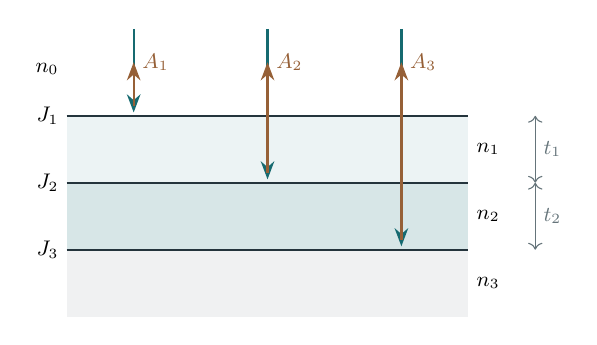
\begin{tikzpicture}[scale=.85,transform shape]

\fill[accent!8] (-3,1) rectangle (3,2);
\fill[accent!17] (-3,0) rectangle (3,1);
\fill[muted!10] (-3,-1) rectangle (3,0);
\foreach \y/\p in {2/J_1,1/J_2,0/J_3}{\draw[object] (-3,\y)--(3,\y);\node[left] at (-3,\y) {$\p$};}
\node[left] at (-3,2.7) {$n_0$};
\node[right] at (3,1.5) {$n_1$};\node[right] at (3,.5) {$n_2$};
\node[right] at (3,-.5) {$n_3$};
\draw[axis,<->] (4,1)--(4,2) node[midway,right] {$t_1$};
\draw[axis,<->] (4,0)--(4,1) node[midway,right] {$t_2$};
\draw[motion] (-2,3.3)--(-2,2.05);
\draw[motion] (0,3.3)--(0,1.05);
\draw[motion] (2,3.3)--(2,.05);
\draw[force] (-2,2.15)--(-2,2.8) node[right] {$A_1$};
\draw[force] (0,1.15)--(0,2.8) node[right] {$A_2$};
\draw[force] (2,.15)--(2,2.8) node[right] {$A_3$};

\end{tikzpicture}
\figcaption{图光试.5\quad 三条法向反射路径分列表示，$n_0<n_1<n_2,\ n_2>n_3$。}
\end{minipage}\end{center}

\Needspace{8\baselineskip}

\pdfbookmark[3]{题型定位}{q5-h0}

\subsection*{题型定位}

三束等振幅反射光的零和条件与两层膜厚的有序最小化。先把界面反射相变与传播相位写进同一个复振幅式，再列出两族厚度，按先$t_1$后$t_2$的次序选支。

\Needspace{8\baselineskip}

\pdfbookmark[3]{知识点}{q5-h1}

\subsection*{知识点}

低折射率向高折射率反射的电场振幅变号，高向低反射相位保持；两层往返传播相位分别为$4\pi n_jt_j/\lambda$。三条等长相量零和时方向相隔$120^\circ$，可画成首尾闭合等边三角形。取模方程先确定$\delta_1$的两种相位，再回代决定$\delta_2$。每层厚度可独立增加$\lambda/(2n_j)$，形成全部正厚度解。题设规定三束共同振幅，参与求和的分量为三个界面的一次反射光。

\Needspace{8\baselineskip}

\pdfbookmark[3]{物理图像}{q5-h2}

\subsection*{物理图像}

解图光试.5A沿三条回程标出界面相变$\pi,\pi,0$；第一束作相位参考后，第三束带相对负号。解图B将公共起点的三个相量和首尾相接的闭合三角形并列，方向角与求和对应。解图C把往返光程$\lambda/3$、$5\lambda/6$换成传播相位，累计到第三束后再加入反射相位差。

\Needspace{8\baselineskip}

\pdfbookmark[3]{解题入口}{q5-h3}

\subsection*{解题入口}

统一参考面，记两层往返传播相位为$\delta_1,\delta_2$，将公共第一束相位除去。由$1+e^{\mathrm j\delta_1}=e^{\mathrm j(\delta_1+\delta_2)}$取模，得到$\cos\delta_1=-1/2$。分别计算$1+e^{2\pi\mathrm j/3}$与$1+e^{4\pi\mathrm j/3}$的辐角，再回代第二层相位；列全两族后比较第一层厚度。

\Needspace{8\baselineskip}

\pdfbookmark[3]{标准解法}{q5-h4}

\subsection*{标准解法}


图光试.5的三个界面分别记为$J_1,J_2,J_3$。从低折射率入射到高折射率的反射振幅变号，相位增加$\pi$；从高到低反射不增加该相位。因此三次反射附加相位依次为
\[
\pi,\qquad \pi,\qquad 0.
\]
\begin{center}\begin{minipage}{.98\linewidth}\centering
\begin{tikzpicture}[scale=.7,transform shape]

\fill[accent!8] (-3,1) rectangle (3,2);
\fill[accent!17] (-3,0) rectangle (3,1);
\fill[muted!10] (-3,-1) rectangle (3,0);
\foreach \y/\p in {2/J_1,1/J_2,0/J_3}{\draw[object] (-3,\y)--(3,\y);\node[left] at (-3,\y) {$\p$};}
\node[left] at (-3,2.7) {$n_0$};
\node[right] at (3,1.5) {$n_1$};\node[right] at (3,.5) {$n_2$};
\node[right] at (3,-.5) {$n_3$};
\draw[axis,<->] (4,1)--(4,2) node[midway,right] {$t_1$};
\draw[axis,<->] (4,0)--(4,1) node[midway,right] {$t_2$};
\draw[motion] (-2,3.3)--(-2,2.05);
\draw[motion] (0,3.3)--(0,1.05);
\draw[motion] (2,3.3)--(2,.05);
\draw[force] (-2,2.15)--(-2,2.8) node[right] {$A_1$};
\draw[force] (0,1.15)--(0,2.8) node[right] {$A_2$};
\draw[force] (2,.15)--(2,2.8) node[right] {$A_3$};

\node[align=left] at (8,2) {$J_1:\ \pi$\\$J_2:\ \pi$\\$J_3:\ 0$};
\node[align=left] at (8,0) {第二束往返：$2n_1t_1$\\第三束往返：$2n_1t_1+2n_2t_2$};

\end{tikzpicture}
\figcaption{解图光试.5A\quad 三界面的反射相变与两层往返传播相位分别计入，第三束带相对负号。}
\end{minipage}\end{center}
解图光试.5A把第二、三束在膜内的往返路程分别标为$2n_1t_1$与$2n_1t_1+2n_2t_2$。令
\[
\delta_1=\frac{4\pi n_1t_1}{\lambda},\qquad
\delta_2=\frac{4\pi n_2t_2}{\lambda}.
\]
去掉公共的第一束相位，并取三束共同振幅为$A>0$，复振幅可写成
\[
\widetilde A_1=A,\qquad
\widetilde A_2=Ae^{\mathrm j\delta_1},\qquad
\widetilde A_3=-Ae^{\mathrm j(\delta_1+\delta_2)}.
\]
第三束前的负号保留了它与前两束反射相位相差$\pi$这一事实。要求总强度为零，就是
\[
1+e^{\mathrm j\delta_1}
-e^{\mathrm j(\delta_1+\delta_2)}=0.
\]
\begin{center}\begin{minipage}{.98\linewidth}\centering
\begin{tikzpicture}[scale=.8,transform shape]

\draw[motion] (0,0)--(2,0) node[right] {$A_1$};
\draw[motion] (0,0)--(-1,1.732) node[above] {$A_2$};
\draw[motion] (0,0)--(-1,-1.732) node[below] {$A_3$};
\draw[guide] (0,0) circle (2);
\node at (0,3) {共同起点：相位相隔$120^\circ$};
\begin{scope}[xshift=6cm]
\draw[motion] (0,0)--(2,0) node[midway,below] {$A_1$};
\draw[motion] (2,0)--(1,1.732) node[midway,right] {$A_2$};
\draw[motion] (1,1.732)--(0,0) node[midway,left] {$A_3$};
\node at (1,3) {首尾闭合：合振幅为零};
\end{scope}
\node at (3,-3) {$\delta_1=2\pi/3,\quad\delta_2=5\pi/3$时的三相量};

\end{tikzpicture}
\figcaption{解图光试.5B\quad 方向角与矢量首尾相加是同一零和条件的两种画法。}
\end{minipage}\end{center}
解图光试.5B中三条等长相量在零和时首尾组成等边三角形，等价于从共同起点画出时方向依次相差$120^\circ$。对零和方程取模，可具体求得：
\[
|1+e^{\mathrm j\delta_1}|^2=1
\quad\Longrightarrow\quad
2+2\cos\delta_1=1.
\]
所以$\cos\delta_1=-1/2$，在模$2\pi$意义下只有
\[
\delta_1\equiv\frac{2\pi}{3}\quad\text{或}\quad
\delta_1\equiv\frac{4\pi}{3}.
\]
对第一支$\delta_1=2\pi/3$，$1+e^{2\pi\mathrm j/3}=e^{\pi\mathrm j/3}$，故$\delta_1+\delta_2\equiv\pi/3$，得到$\delta_2\equiv5\pi/3$。对第二支$\delta_1=4\pi/3$，和为$e^{-\pi\mathrm j/3}$，所以$\delta_2\equiv\pi/3$。每一层增加$\lambda/(2n)$只使相应传播相位增加$2\pi$。分别加上独立的整周期后，得到两族正厚度解：
\[
\begin{array}{c|c|c}
&t_1&t_2\\ \hline
\text{第一族}&\displaystyle\frac{\lambda}{6n_1}
+m\frac{\lambda}{2n_1}
&\displaystyle\frac{5\lambda}{12n_2}
+p\frac{\lambda}{2n_2}\\[2mm]
\text{第二族}&\displaystyle\frac{\lambda}{3n_1}
+m\frac{\lambda}{2n_1}
&\displaystyle\frac{\lambda}{12n_2}
+p\frac{\lambda}{2n_2}
\end{array}
\qquad m,p=0,1,2,\ldots.
\]
例如第一族的最小相位为$\delta_1=2\pi/3$、$\delta_2=5\pi/3$，第三束相对于第一束的总相位为
$\delta_1+\delta_2+\pi\equiv4\pi/3$，三束相位正是$0,2\pi/3,4\pi/3$。

按题意先最小化$t_1$，第一族给出的$\lambda/(6n_1)$小于第二族的$\lambda/(3n_1)$；再在第一族内取$p=0$，故
\[
\boxed{t_{1,\min}=\frac{\lambda}{6n_1},\qquad
t_{2,\min\,|\,t_{1,\min}}=\frac{5\lambda}{12n_2}}.
\]
单独追求$t_2$最小则应选第二族，$t_2=\lambda/(12n_2)$，同时$t_1=\lambda/(3n_1)$。两层的厚度由同一支相位条件配对。若比较两组总厚度，第二族的最小总厚度减去第一族的最小总厚度为
\[
\left(\frac{\lambda}{3n_1}+\frac{\lambda}{12n_2}\right)
-\left(\frac{\lambda}{6n_1}+\frac{5\lambda}{12n_2}\right)
=\frac{\lambda(n_2-2n_1)}{6n_1n_2}.
\]
所以 $n_2<2n_1$ 时，先使 $t_2$ 最小所得组合的总厚度也较小；$n_2=2n_1$ 时总厚度相同；$n_2>2n_1$ 时，先使 $t_1$ 最小所得组合的总厚度较小。

题设将三个一次反射分量的共同幅度规定为$A$。若考虑其余多次往返或改变三个幅度，便以对应传播和反射系数构成全部复振幅之和；膜厚扰动时，各层传播相位按$4\pi n_jt_j/\lambda$随厚度改变。
还可把第一族写成直观的光程式：$2n_1t_1=\lambda/3$，而第一、第三束的反射相位相差$\pi$，故$2n_1t_1+2n_2t_2=7\lambda/6$；相减得到$2n_2t_2=5\lambda/6$。解图光试.5C按这两个往返光程画出相位逐段累积。
\begin{center}\begin{minipage}{.98\linewidth}\centering
\begin{tikzpicture}[scale=0.72,transform shape]
\draw[axis] (0,0)--(6.2,0);\draw[axis] (0,0)--(0,3.4000000000000004);
\draw[thin,color=muted] (0.0000000,0)--(0.0000000,-.07);\node[below] at (0.0000000,-.09) {参考};
\draw[thin,color=muted] (2.0000000,0)--(2.0000000,-.07);\node[below] at (2.0000000,-.09) {第一层往返};
\draw[thin,color=muted] (4.0000000,0)--(4.0000000,-.07);\node[below] at (4.0000000,-.09) {第二层往返};
\draw[thin,color=muted] (6.0000000,0)--(6.0000000,-.07);\node[below] at (6.0000000,-.09) {相对反射};
\draw[thin,color=muted] (0,0.0000000)--(-.07,0.0000000);\node[left] at (-.09,0.0000000) {$0$};
\draw[thin,color=muted] (0,0.5925926)--(-.07,0.5925926);\node[left] at (-.09,0.5925926) {$2/3$};
\draw[thin,color=muted] (0,2.0740741)--(-.07,2.0740741);\node[left] at (-.09,2.0740741) {$7/3$};
\draw[thin,color=muted] (0,2.9629630)--(-.07,2.9629630);\node[left] at (-.09,2.9629630) {$10/3$};
\node[below] at (3.0,-.64) {逐段累计};\node[above right] at (0,3.45) {相位除以$\pi$};
\draw[traj] plot coordinates {(0.0000000,0.0000000) (2.0000000,0.5925926) (4.0000000,2.0740741) (6.0000000,2.9629630)};
\draw[traj] (.1,-1.05)--(.7,-1.05);\node[right] at (.85,-1.05) {第三束传播与相对反射相位};\end{tikzpicture}
\figcaption{解图光试.5C\quad 传播相位之和为 $7\pi/3$，再计相对反射 $\pi$ 后等效方向为 $4\pi/3$}
\end{minipage}\end{center}


\Needspace{8\baselineskip}

\pdfbookmark[3]{关键洞察}{q5-h5}

\subsection*{关键洞察}

最小第一层取$\delta_1=2\pi/3$，对应第二层传播相位$5\pi/3$。另一族的第二层更薄，却配合较厚的第一层。两族各自满足完整复振幅方程，独立选取两个较小厚度会改变相量闭合关系。反射相变决定传播相位应选哪个支，而整周期增加保持零和。

\Needspace{8\baselineskip}

\pdfbookmark[3]{易错点}{q5-h6}

\subsection*{易错点}

第一、第二界面反射相变相同，第三界面与它们相差$\pi$，这个相对符号保留在第三束前。厚度进入往返光程$2nt$。公共起点相量相隔$120^\circ$与首尾相接三角形的内角$60^\circ$对应不同画法。两层相位求解先后相关，而整周期次数可以独立增加。等幅以外的三束相消由三角形边长关系决定。

\Needspace{8\baselineskip}

\pdfbookmark[3]{课堂讲解建议}{q5-h7}

\subsection*{课堂讲解建议}

让学生先在膜的三个界面写反射相位，再给每条出射光标往返路径。随后画三个单位相量，要求用复数取模代数说明为何只有两支。两组学生分别求一支，集中比较先$t_1$与先$t_2$的结果。把两支中各自较薄的厚度拼合，实际计算其复振幅残量，说明厚度优化的先后约束。最后改变某一层厚度一个小量，联系变式中的残余强度与制造误差。

\Needspace{8\baselineskip}

\pdfbookmark[3]{变式训练}{q5-h8}

\subsection*{变式训练}

\begin{enumerate}
\Needspace{37\baselineskip}
\item \textbf{题设与求解。} 改为先使$t_2$最小，再在该条件下选最小$t_1$。两族中，第二族的$t_2=\lambda/(12n_2)$较小，同时$t_1=\lambda/(3n_1)$。此时$\delta_1=4\pi/3$、$\delta_2=\pi/3$，第三束实际相位为$\delta_1+\delta_2+\pi\equiv2\pi/3$。三束方向仍为$0,4\pi/3,2\pi/3$，总和为零。解图光试.5V1将这组相量与第一族比较，三束后两条的方向互换。
\begin{center}\begin{minipage}{.98\linewidth}\centering
\begin{tikzpicture}[scale=0.9,transform shape]
\draw[motion] (0,0)--(2.00000000,0.00000000) node[above] {$A_1$};\draw[force] (0,0)--(-1.00000000,-1.73205081) node[below] {$A_2$};\draw[traj] (0,0)--(-1.00000000,1.73205081) node[above] {$A_3$};\end{tikzpicture}
\figcaption{解图光试.5V1\quad 先最小化第二层时后两相量方向互换，仍然等长零和}
\end{minipage}\end{center}
\Needspace{37\baselineskip}
\item \textbf{题设与求解。} 从任意一组零反射厚度出发，分别增加$\Delta t_1=m\lambda/(2n_1)$和$\Delta t_2=p\lambda/(2n_2)$，$m,p$为非负整数，说明结果。两传播相位分别增加$2\pi m$与$2\pi p$，所以第二束乘$e^{2\pi m\mathrm j}=1$，第三束乘$e^{2\pi(m+p)\mathrm j}=1$，总振幅保持不变。解图光试.5V2在归一化厚度平面$(n_1t_1/\lambda,n_2t_2/\lambda)$上画出两族格点，间隔均为$1/2$；同一族两个周期数相互独立。
\begin{center}\begin{minipage}{.98\linewidth}\centering
\begin{tikzpicture}[scale=0.72,transform shape]
\draw[axis] (0,0)--(6.2,0);\draw[axis] (0,0)--(0,3.4000000000000004);
\draw[thin,color=muted] (0.0000000,0)--(0.0000000,-.07);\node[below] at (0.0000000,-.09) {$0$};
\draw[thin,color=muted] (1.8750000,0)--(1.8750000,-.07);\node[below] at (1.8750000,-.09) {$.5$};
\draw[thin,color=muted] (3.7500000,0)--(3.7500000,-.07);\node[below] at (3.7500000,-.09) {$1$};
\draw[thin,color=muted] (5.6250000,0)--(5.6250000,-.07);\node[below] at (5.6250000,-.09) {$1.5$};
\draw[thin,color=muted] (0,0.0000000)--(-.07,0.0000000);\node[left] at (-.09,0.0000000) {$0$};
\draw[thin,color=muted] (0,1.0000000)--(-.07,1.0000000);\node[left] at (-.09,1.0000000) {$.5$};
\draw[thin,color=muted] (0,2.0000000)--(-.07,2.0000000);\node[left] at (-.09,2.0000000) {$1$};
\draw[thin,color=muted] (0,3.0000000)--(-.07,3.0000000);\node[left] at (-.09,3.0000000) {$1.5$};
\node[below] at (3.0,-.64) {$n_1t_1/\lambda$};\node[above right] at (0,3.45) {$n_2t_2/\lambda$};
\fill[color=accent] (0.62500000,0.83333333) circle(.045);\fill[color=accent] (0.62500000,1.83333333) circle(.045);\fill[color=accent] (0.62500000,2.83333333) circle(.045);\fill[color=accent] (2.50000000,0.83333333) circle(.045);\fill[color=accent] (2.50000000,1.83333333) circle(.045);\fill[color=accent] (2.50000000,2.83333333) circle(.045);\fill[color=accent] (4.37500000,0.83333333) circle(.045);\fill[color=accent] (4.37500000,1.83333333) circle(.045);\fill[color=accent] (4.37500000,2.83333333) circle(.045);\fill[color=warm] (1.25000000,0.16666667) circle(.045);\fill[color=warm] (1.25000000,1.16666667) circle(.045);\fill[color=warm] (1.25000000,2.16666667) circle(.045);\fill[color=warm] (3.12500000,0.16666667) circle(.045);\fill[color=warm] (3.12500000,1.16666667) circle(.045);\fill[color=warm] (3.12500000,2.16666667) circle(.045);\fill[color=warm] (5.00000000,0.16666667) circle(.045);\fill[color=warm] (5.00000000,1.16666667) circle(.045);\fill[color=warm] (5.00000000,2.16666667) circle(.045);\node[below] at (3,-1) {青色：第一族；棕色：第二族；周期数独立增加};\end{tikzpicture}
\figcaption{解图光试.5V2\quad 正厚度解在两层归一化厚度平面中形成两套格点}
\end{minipage}\end{center}
\Needspace{37\baselineskip}
\item \textbf{题设与求解。} 第一族零反射膜仅第一层偏厚$\epsilon$，求残余反射强度。令$\eta=4\pi n_1\epsilon/\lambda$，第二、第三束都多走第一层往返，因而共同乘$e^{\mathrm j\eta}$。设计状态下两束之和为$-A$，新总振幅为$A(1-e^{\mathrm j\eta})$，
\[
I=4A^2\sin^2(\eta/2)=A^2\eta^2+O(\eta^4).
\]
解图光试.5V3同时画精确强度和二次近似。厚度误差变为两倍时，小误差区的残余强度约为四倍。
\begin{center}\begin{minipage}{.98\linewidth}\centering
\begin{tikzpicture}[scale=0.72,transform shape]
\draw[axis] (0,0)--(6.2,0);\draw[axis] (0,0)--(0,3.4000000000000004);
\draw[thin,color=muted] (0.0000000,0)--(0.0000000,-.07);\node[below] at (0.0000000,-.09) {$-.4$};
\draw[thin,color=muted] (3.0000000,0)--(3.0000000,-.07);\node[below] at (3.0000000,-.09) {$0$};
\draw[thin,color=muted] (6.0000000,0)--(6.0000000,-.07);\node[below] at (6.0000000,-.09) {$.4$};
\draw[thin,color=muted] (0,0.0000000)--(-.07,0.0000000);\node[left] at (-.09,0.0000000) {$0$};
\draw[thin,color=muted] (0,1.5058824)--(-.07,1.5058824);\node[left] at (-.09,1.5058824) {$.08$};
\draw[thin,color=muted] (0,3.0117647)--(-.07,3.0117647);\node[left] at (-.09,3.0117647) {$.16$};
\node[below] at (3.0,-.64) {第一层相位误差$\eta$};\node[above right] at (0,3.45) {$I/A^2$};
\draw[traj] plot coordinates {(0.0000000,2.9718214) (0.0250000,2.9231459) (0.0500000,2.8748563) (0.0750000,2.8269530) (0.1000000,2.7794367) (0.1250000,2.7323077) (0.1500000,2.6855667) (0.1750000,2.6392141) (0.2000000,2.5932505) (0.2250000,2.5476764) (0.2500000,2.5024923) (0.2750000,2.4576987) (0.3000000,2.4132960) (0.3250000,2.3692849) (0.3500000,2.3256657) (0.3750000,2.2824390) (0.4000000,2.2396053) (0.4250000,2.1971649) (0.4500000,2.1551185) (0.4750000,2.1134664) (0.5000000,2.0722091) (0.5250000,2.0313471) (0.5500000,1.9908808) (0.5750000,1.9508107) (0.6000000,1.9111372) (0.6250000,1.8718608) (0.6500000,1.8329819) (0.6750000,1.7945009) (0.7000000,1.7564183) (0.7250000,1.7187344) (0.7500000,1.6814498) (0.7750000,1.6445648) (0.8000000,1.6080798) (0.8250000,1.5719953) (0.8500000,1.5363116) (0.8750000,1.5010291) (0.9000000,1.4661482) (0.9250000,1.4316693) (0.9500000,1.3975929) (0.9750000,1.3639192) (1.0000000,1.3306487) (1.0250000,1.2977816) (1.0500000,1.2653185) (1.0750000,1.2332596) (1.1000000,1.2016053) (1.1250000,1.1703559) (1.1500000,1.1395118) (1.1750000,1.1090734) (1.2000000,1.0790409) (1.2250000,1.0494148) (1.2500000,1.0201953) (1.2750000,0.9913828) (1.3000000,0.9629775) (1.3250000,0.9349799) (1.3500000,0.9073901) (1.3750000,0.8802086) (1.4000000,0.8534356) (1.4250000,0.8270714) (1.4500000,0.8011164) (1.4750000,0.7755707) (1.5000000,0.7504347) (1.5250000,0.7257087) (1.5500000,0.7013929) (1.5750000,0.6774876) (1.6000000,0.6539931) (1.6250000,0.6309096) (1.6500000,0.6082374) (1.6750000,0.5859768) (1.7000000,0.5641280) (1.7250000,0.5426911) (1.7500000,0.5216666) (1.7750000,0.5010545) (1.8000000,0.4808552) (1.8250000,0.4610689) (1.8500000,0.4416957) (1.8750000,0.4227359) (1.9000000,0.4041897) (1.9250000,0.3860573) (1.9500000,0.3683390) (1.9750000,0.3510348) (2.0000000,0.3341451) (2.0250000,0.3176699) (2.0500000,0.3016095) (2.0750000,0.2859640) (2.1000000,0.2707337) (2.1250000,0.2559187) (2.1500000,0.2415191) (2.1750000,0.2275351) (2.2000000,0.2139669) (2.2250000,0.2008147) (2.2500000,0.1880785) (2.2750000,0.1757585) (2.3000000,0.1638549) (2.3250000,0.1523677) (2.3500000,0.1412971) (2.3750000,0.1306433) (2.4000000,0.1204064) (2.4250000,0.1105863) (2.4500000,0.1011834) (2.4750000,0.0921976) (2.5000000,0.0836292) (2.5250000,0.0754780) (2.5500000,0.0677444) (2.5750000,0.0604283) (2.6000000,0.0535298) (2.6250000,0.0470490) (2.6500000,0.0409860) (2.6750000,0.0353409) (2.7000000,0.0301136) (2.7250000,0.0253044) (2.7500000,0.0209131) (2.7750000,0.0169399) (2.8000000,0.0133848) (2.8250000,0.0102479) (2.8500000,0.0075292) (2.8750000,0.0052286) (2.9000000,0.0033464) (2.9250000,0.0018823) (2.9500000,0.0008366) (2.9750000,0.0002092) (3.0000000,0.0000000) (3.0250000,0.0002092) (3.0500000,0.0008366) (3.0750000,0.0018823) (3.1000000,0.0033464) (3.1250000,0.0052286) (3.1500000,0.0075292) (3.1750000,0.0102479) (3.2000000,0.0133848) (3.2250000,0.0169399) (3.2500000,0.0209131) (3.2750000,0.0253044) (3.3000000,0.0301136) (3.3250000,0.0353409) (3.3500000,0.0409860) (3.3750000,0.0470490) (3.4000000,0.0535298) (3.4250000,0.0604283) (3.4500000,0.0677444) (3.4750000,0.0754780) (3.5000000,0.0836292) (3.5250000,0.0921976) (3.5500000,0.1011834) (3.5750000,0.1105863) (3.6000000,0.1204064) (3.6250000,0.1306433) (3.6500000,0.1412971) (3.6750000,0.1523677) (3.7000000,0.1638549) (3.7250000,0.1757585) (3.7500000,0.1880785) (3.7750000,0.2008147) (3.8000000,0.2139669) (3.8250000,0.2275351) (3.8500000,0.2415191) (3.8750000,0.2559187) (3.9000000,0.2707337) (3.9250000,0.2859640) (3.9500000,0.3016095) (3.9750000,0.3176699) (4.0000000,0.3341451) (4.0250000,0.3510348) (4.0500000,0.3683390) (4.0750000,0.3860573) (4.1000000,0.4041897) (4.1250000,0.4227359) (4.1500000,0.4416957) (4.1750000,0.4610689) (4.2000000,0.4808552) (4.2250000,0.5010545) (4.2500000,0.5216666) (4.2750000,0.5426911) (4.3000000,0.5641280) (4.3250000,0.5859768) (4.3500000,0.6082374) (4.3750000,0.6309096) (4.4000000,0.6539931) (4.4250000,0.6774876) (4.4500000,0.7013929) (4.4750000,0.7257087) (4.5000000,0.7504347) (4.5250000,0.7755707) (4.5500000,0.8011164) (4.5750000,0.8270714) (4.6000000,0.8534356) (4.6250000,0.8802086) (4.6500000,0.9073901) (4.6750000,0.9349799) (4.7000000,0.9629775) (4.7250000,0.9913828) (4.7500000,1.0201953) (4.7750000,1.0494148) (4.8000000,1.0790409) (4.8250000,1.1090734) (4.8500000,1.1395118) (4.8750000,1.1703559) (4.9000000,1.2016053) (4.9250000,1.2332596) (4.9500000,1.2653185) (4.9750000,1.2977816) (5.0000000,1.3306487) (5.0250000,1.3639192) (5.0500000,1.3975929) (5.0750000,1.4316693) (5.1000000,1.4661482) (5.1250000,1.5010291) (5.1500000,1.5363116) (5.1750000,1.5719953) (5.2000000,1.6080798) (5.2250000,1.6445648) (5.2500000,1.6814498) (5.2750000,1.7187344) (5.3000000,1.7564183) (5.3250000,1.7945009) (5.3500000,1.8329819) (5.3750000,1.8718608) (5.4000000,1.9111372) (5.4250000,1.9508107) (5.4500000,1.9908808) (5.4750000,2.0313471) (5.5000000,2.0722091) (5.5250000,2.1134664) (5.5500000,2.1551185) (5.5750000,2.1971649) (5.6000000,2.2396053) (5.6250000,2.2824390) (5.6500000,2.3256657) (5.6750000,2.3692849) (5.7000000,2.4132960) (5.7250000,2.4576987) (5.7500000,2.5024923) (5.7750000,2.5476764) (5.8000000,2.5932505) (5.8250000,2.6392141) (5.8500000,2.6855667) (5.8750000,2.7323077) (5.9000000,2.7794367) (5.9250000,2.8269530) (5.9500000,2.8748563) (5.9750000,2.9231459) (6.0000000,2.9718214)};
\draw[traj] (.1,-1.05)--(.7,-1.05);\node[right] at (.85,-1.05) {精确强度};\draw[dashed,thick,color=warm] plot coordinates {(0.0000000,3.0117647) (0.0250000,2.9617778) (0.0500000,2.9122092) (0.0750000,2.8630588) (0.1000000,2.8143268) (0.1250000,2.7660131) (0.1500000,2.7181176) (0.1750000,2.6706405) (0.2000000,2.6235817) (0.2250000,2.5769412) (0.2500000,2.5307190) (0.2750000,2.4849150) (0.3000000,2.4395294) (0.3250000,2.3945621) (0.3500000,2.3500131) (0.3750000,2.3058824) (0.4000000,2.2621699) (0.4250000,2.2188758) (0.4500000,2.1760000) (0.4750000,2.1335425) (0.5000000,2.0915033) (0.5250000,2.0498824) (0.5500000,2.0086797) (0.5750000,1.9678954) (0.6000000,1.9275294) (0.6250000,1.8875817) (0.6500000,1.8480523) (0.6750000,1.8089412) (0.7000000,1.7702484) (0.7250000,1.7319739) (0.7500000,1.6941176) (0.7750000,1.6566797) (0.8000000,1.6196601) (0.8250000,1.5830588) (0.8500000,1.5468758) (0.8750000,1.5111111) (0.9000000,1.4757647) (0.9250000,1.4408366) (0.9500000,1.4063268) (0.9750000,1.3722353) (1.0000000,1.3385621) (1.0250000,1.3053072) (1.0500000,1.2724706) (1.0750000,1.2400523) (1.1000000,1.2080523) (1.1250000,1.1764706) (1.1500000,1.1453072) (1.1750000,1.1145621) (1.2000000,1.0842353) (1.2250000,1.0543268) (1.2500000,1.0248366) (1.2750000,0.9957647) (1.3000000,0.9671111) (1.3250000,0.9388758) (1.3500000,0.9110588) (1.3750000,0.8836601) (1.4000000,0.8566797) (1.4250000,0.8301176) (1.4500000,0.8039739) (1.4750000,0.7782484) (1.5000000,0.7529412) (1.5250000,0.7280523) (1.5500000,0.7035817) (1.5750000,0.6795294) (1.6000000,0.6558954) (1.6250000,0.6326797) (1.6500000,0.6098824) (1.6750000,0.5875033) (1.7000000,0.5655425) (1.7250000,0.5440000) (1.7500000,0.5228758) (1.7750000,0.5021699) (1.8000000,0.4818824) (1.8250000,0.4620131) (1.8500000,0.4425621) (1.8750000,0.4235294) (1.9000000,0.4049150) (1.9250000,0.3867190) (1.9500000,0.3689412) (1.9750000,0.3515817) (2.0000000,0.3346405) (2.0250000,0.3181176) (2.0500000,0.3020131) (2.0750000,0.2863268) (2.1000000,0.2710588) (2.1250000,0.2562092) (2.1500000,0.2417778) (2.1750000,0.2277647) (2.2000000,0.2141699) (2.2250000,0.2009935) (2.2500000,0.1882353) (2.2750000,0.1758954) (2.3000000,0.1639739) (2.3250000,0.1524706) (2.3500000,0.1413856) (2.3750000,0.1307190) (2.4000000,0.1204706) (2.4250000,0.1106405) (2.4500000,0.1012288) (2.4750000,0.0922353) (2.5000000,0.0836601) (2.5250000,0.0755033) (2.5500000,0.0677647) (2.5750000,0.0604444) (2.6000000,0.0535425) (2.6250000,0.0470588) (2.6500000,0.0409935) (2.6750000,0.0353464) (2.7000000,0.0301176) (2.7250000,0.0253072) (2.7500000,0.0209150) (2.7750000,0.0169412) (2.8000000,0.0133856) (2.8250000,0.0102484) (2.8500000,0.0075294) (2.8750000,0.0052288) (2.9000000,0.0033464) (2.9250000,0.0018824) (2.9500000,0.0008366) (2.9750000,0.0002092) (3.0000000,0.0000000) (3.0250000,0.0002092) (3.0500000,0.0008366) (3.0750000,0.0018824) (3.1000000,0.0033464) (3.1250000,0.0052288) (3.1500000,0.0075294) (3.1750000,0.0102484) (3.2000000,0.0133856) (3.2250000,0.0169412) (3.2500000,0.0209150) (3.2750000,0.0253072) (3.3000000,0.0301176) (3.3250000,0.0353464) (3.3500000,0.0409935) (3.3750000,0.0470588) (3.4000000,0.0535425) (3.4250000,0.0604444) (3.4500000,0.0677647) (3.4750000,0.0755033) (3.5000000,0.0836601) (3.5250000,0.0922353) (3.5500000,0.1012288) (3.5750000,0.1106405) (3.6000000,0.1204706) (3.6250000,0.1307190) (3.6500000,0.1413856) (3.6750000,0.1524706) (3.7000000,0.1639739) (3.7250000,0.1758954) (3.7500000,0.1882353) (3.7750000,0.2009935) (3.8000000,0.2141699) (3.8250000,0.2277647) (3.8500000,0.2417778) (3.8750000,0.2562092) (3.9000000,0.2710588) (3.9250000,0.2863268) (3.9500000,0.3020131) (3.9750000,0.3181176) (4.0000000,0.3346405) (4.0250000,0.3515817) (4.0500000,0.3689412) (4.0750000,0.3867190) (4.1000000,0.4049150) (4.1250000,0.4235294) (4.1500000,0.4425621) (4.1750000,0.4620131) (4.2000000,0.4818824) (4.2250000,0.5021699) (4.2500000,0.5228758) (4.2750000,0.5440000) (4.3000000,0.5655425) (4.3250000,0.5875033) (4.3500000,0.6098824) (4.3750000,0.6326797) (4.4000000,0.6558954) (4.4250000,0.6795294) (4.4500000,0.7035817) (4.4750000,0.7280523) (4.5000000,0.7529412) (4.5250000,0.7782484) (4.5500000,0.8039739) (4.5750000,0.8301176) (4.6000000,0.8566797) (4.6250000,0.8836601) (4.6500000,0.9110588) (4.6750000,0.9388758) (4.7000000,0.9671111) (4.7250000,0.9957647) (4.7500000,1.0248366) (4.7750000,1.0543268) (4.8000000,1.0842353) (4.8250000,1.1145621) (4.8500000,1.1453072) (4.8750000,1.1764706) (4.9000000,1.2080523) (4.9250000,1.2400523) (4.9500000,1.2724706) (4.9750000,1.3053072) (5.0000000,1.3385621) (5.0250000,1.3722353) (5.0500000,1.4063268) (5.0750000,1.4408366) (5.1000000,1.4757647) (5.1250000,1.5111111) (5.1500000,1.5468758) (5.1750000,1.5830588) (5.2000000,1.6196601) (5.2250000,1.6566797) (5.2500000,1.6941176) (5.2750000,1.7319739) (5.3000000,1.7702484) (5.3250000,1.8089412) (5.3500000,1.8480523) (5.3750000,1.8875817) (5.4000000,1.9275294) (5.4250000,1.9678954) (5.4500000,2.0086797) (5.4750000,2.0498824) (5.5000000,2.0915033) (5.5250000,2.1335425) (5.5500000,2.1760000) (5.5750000,2.2188758) (5.6000000,2.2621699) (5.6250000,2.3058824) (5.6500000,2.3500131) (5.6750000,2.3945621) (5.7000000,2.4395294) (5.7250000,2.4849150) (5.7500000,2.5307190) (5.7750000,2.5769412) (5.8000000,2.6235817) (5.8250000,2.6706405) (5.8500000,2.7181176) (5.8750000,2.7660131) (5.9000000,2.8143268) (5.9250000,2.8630588) (5.9500000,2.9122092) (5.9750000,2.9617778) (6.0000000,3.0117647)};
\draw[dashed,thick,color=warm] (.1,-1.5)--(.7,-1.5);\node[right] at (.85,-1.5) {二次近似};\end{tikzpicture}
\figcaption{解图光试.5V3\quad 第一层厚度微扰使第二、第三相量共同旋转}
\end{minipage}\end{center}
\Needspace{37\baselineskip}
\item \textbf{题设与求解。} 三振幅大小为$A_1,A_2,A_3$时，何时能通过调相完全相消？三个矢量能首尾闭合的充要条件为最大边长不大于另两者之和。令$A_1$沿实轴，$A_2$的方向角为$\phi$，则$|A_1+A_2e^{\mathrm j\phi}|=A_3$，所以
\[
\cos\phi=\frac{A_3^2-A_1^2-A_2^2}{2A_1A_2}.
\]
取$A_1=A_2=1,A_3=1.5$，得$\cos\phi=1/8$、$\phi\simeq82.819^\circ$；第三相量方向为$\pi+\phi/2$。对应$\delta_1=\phi$、$\delta_2\equiv-\phi/2\pmod{2\pi}$，由传播相位反求正膜厚即可。图V4画这组三角形，等振幅时才回到等边形。
\begin{center}\begin{minipage}{.98\linewidth}\centering
\begin{tikzpicture}[scale=1.0,transform shape]
\draw[motion] (0,0)--(2,0) node[midway,below] {$A_1=1$};
\draw[force] (2,0)--(2.25000000,1.98431348) node[midway,right] {$A_2=1$};
\draw[motion] (2.25000000,1.98431348)--(0,0) node[midway,above left] {$A_3=1.5$};
\draw[guide] (0,0)--(0.25000000,1.98431348);\node[above] at (.7,.3) {$\phi$};\end{tikzpicture}
\figcaption{解图光试.5V4\quad 不等振幅三角形闭合时，相量方向由实际边长决定}
\end{minipage}\end{center}
\Needspace{37\baselineskip}
\item \textbf{题设与求解。} 仅第二层厚度增加$\epsilon_2$，其余条件保持设计值。只有第三束多走第二层往返，令$\eta_2=4\pi n_2\epsilon_2/\lambda$，残余复振幅为$\widetilde A_3(e^{\mathrm j\eta_2}-1)$。因$|\widetilde A_3|=A$，仍有$I/A^2=4\sin^2(\eta_2/2)$。图V5以相量端点的弦长表示残量，弦长为$2A|\sin(\eta_2/2)|$；强度与第一层同样的相位误差相等，而对应厚度误差按各层$n_j$换算。
\begin{center}\begin{minipage}{.98\linewidth}\centering
\begin{tikzpicture}[scale=0.85,transform shape]
\draw[guide] (0,0) circle(2);\draw[motion] (0,0)--(-1.00000000,-1.73205081) node[below] {$A_3$};\draw[force] (0,0)--(-0.34545629,-1.96993907) node[right] {$A_3e^{\mathrm j\eta_2}$};
\draw[very thick,color=warm] (-1.00000000,-1.73205081)--(-0.34545629,-1.96993907);\node[below] at (0,-2.9) {端点弦长$2A|\sin(\eta_2/2)|$给出残余幅度};\end{tikzpicture}
\figcaption{解图光试.5V5\quad 只改变第二层时，第三相量端点沿圆移动}
\end{minipage}\end{center}
\Needspace{37\baselineskip}
\item \textbf{题设与求解。} 两层都发生小相位误差$\eta_1,\eta_2$，求第一族附近强度的最低阶。记设计相量为$A_1=A$、$A_2=Ae^{2\pi\mathrm j/3}$、$A_3=Ae^{4\pi\mathrm j/3}$，它们之和为零。扰动后总和的一阶为$\mathrm j\eta_1(A_2+A_3)+\mathrm j\eta_2A_3=-\mathrm j\eta_1A+\mathrm j\eta_2A_3$，故
\[
\frac I{A^2}=\eta_1^2+\eta_2^2+\eta_1\eta_2+O(|\eta|^3).
\]
两误差相同时领先项为$3\eta^2$，相反时为$\eta^2$。解图光试.5V6画两条误差路径的强度，交叉项由第一、第三相量的夹角决定。
\begin{center}\begin{minipage}{.98\linewidth}\centering
\begin{tikzpicture}[scale=0.72,transform shape]
\draw[axis] (0,0)--(6.2,0);\draw[axis] (0,0)--(0,3.4000000000000004);
\draw[thin,color=muted] (0.0000000,0)--(0.0000000,-.07);\node[below] at (0.0000000,-.09) {$-.15$};
\draw[thin,color=muted] (3.0000000,0)--(3.0000000,-.07);\node[below] at (3.0000000,-.09) {$0$};
\draw[thin,color=muted] (6.0000000,0)--(6.0000000,-.07);\node[below] at (6.0000000,-.09) {$.15$};
\draw[thin,color=muted] (0,0.0000000)--(-.07,0.0000000);\node[left] at (-.09,0.0000000) {$0$};
\draw[thin,color=muted] (0,1.2800000)--(-.07,1.2800000);\node[left] at (-.09,1.2800000) {$.03$};
\draw[thin,color=muted] (0,2.5600000)--(-.07,2.5600000);\node[left] at (-.09,2.5600000) {$.06$};
\node[below] at (3.0,-.64) {$\eta_1$，且$\eta_2=\pm\eta_1$};\node[above right] at (0,3.45) {$I/A^2$};
\draw[traj] plot coordinates {(0.0000000,3.1118600) (0.0250000,3.0584648) (0.0500000,3.0055577) (0.0750000,2.9531379) (0.1000000,2.9012049) (0.1250000,2.8497580) (0.1500000,2.7987968) (0.1750000,2.7483205) (0.2000000,2.6983285) (0.2250000,2.6488202) (0.2500000,2.5997951) (0.2750000,2.5512524) (0.3000000,2.5031917) (0.3250000,2.4556121) (0.3500000,2.4085132) (0.3750000,2.3618943) (0.4000000,2.3157547) (0.4250000,2.2700938) (0.4500000,2.2249110) (0.4750000,2.1802056) (0.5000000,2.1359770) (0.5250000,2.0922246) (0.5500000,2.0489477) (0.5750000,2.0061456) (0.6000000,1.9638177) (0.6250000,1.9219634) (0.6500000,1.8805819) (0.6750000,1.8396727) (0.7000000,1.7992350) (0.7250000,1.7592683) (0.7500000,1.7197717) (0.7750000,1.6807447) (0.8000000,1.6421866) (0.8250000,1.6040967) (0.8500000,1.5664744) (0.8750000,1.5293189) (0.9000000,1.4926295) (0.9250000,1.4564057) (0.9500000,1.4206466) (0.9750000,1.3853517) (1.0000000,1.3505202) (1.0250000,1.3161514) (1.0500000,1.2822446) (1.0750000,1.2487992) (1.1000000,1.2158144) (1.1250000,1.1832895) (1.1500000,1.1512238) (1.1750000,1.1196166) (1.2000000,1.0884673) (1.2250000,1.0577750) (1.2500000,1.0275391) (1.2750000,0.9977588) (1.3000000,0.9684335) (1.3250000,0.9395624) (1.3500000,0.9111447) (1.3750000,0.8831799) (1.4000000,0.8556670) (1.4250000,0.8286055) (1.4500000,0.8019945) (1.4750000,0.7758334) (1.5000000,0.7501213) (1.5250000,0.7248576) (1.5500000,0.7000415) (1.5750000,0.6756722) (1.6000000,0.6517491) (1.6250000,0.6282713) (1.6500000,0.6052382) (1.6750000,0.5826489) (1.7000000,0.5605027) (1.7250000,0.5387988) (1.7500000,0.5175365) (1.7750000,0.4967151) (1.8000000,0.4763337) (1.8250000,0.4563916) (1.8500000,0.4368880) (1.8750000,0.4178221) (1.9000000,0.3991932) (1.9250000,0.3810006) (1.9500000,0.3632433) (1.9750000,0.3459207) (2.0000000,0.3290319) (2.0250000,0.3125762) (2.0500000,0.2965528) (2.0750000,0.2809608) (2.1000000,0.2657996) (2.1250000,0.2510683) (2.1500000,0.2367661) (2.1750000,0.2228922) (2.2000000,0.2094459) (2.2250000,0.1964262) (2.2500000,0.1838325) (2.2750000,0.1716638) (2.3000000,0.1599195) (2.3250000,0.1485987) (2.3500000,0.1377005) (2.3750000,0.1272242) (2.4000000,0.1171690) (2.4250000,0.1075339) (2.4500000,0.0983183) (2.4750000,0.0895213) (2.5000000,0.0811420) (2.5250000,0.0731797) (2.5500000,0.0656335) (2.5750000,0.0585025) (2.6000000,0.0517860) (2.6250000,0.0454831) (2.6500000,0.0395930) (2.6750000,0.0341149) (2.7000000,0.0290478) (2.7250000,0.0243910) (2.7500000,0.0201436) (2.7750000,0.0163047) (2.8000000,0.0128736) (2.8250000,0.0098493) (2.8500000,0.0072311) (2.8750000,0.0050180) (2.9000000,0.0032092) (2.9250000,0.0018039) (2.9500000,0.0008012) (2.9750000,0.0002001) (3.0000000,0.0000000) (3.0250000,0.0001999) (3.0500000,0.0007988) (3.0750000,0.0017961) (3.1000000,0.0031907) (3.1250000,0.0049819) (3.1500000,0.0071687) (3.1750000,0.0097503) (3.2000000,0.0127258) (3.2250000,0.0160943) (3.2500000,0.0198549) (3.2750000,0.0240068) (3.3000000,0.0285490) (3.3250000,0.0334807) (3.3500000,0.0388010) (3.3750000,0.0445089) (3.4000000,0.0506037) (3.4250000,0.0570844) (3.4500000,0.0639501) (3.4750000,0.0711999) (3.5000000,0.0788330) (3.5250000,0.0868483) (3.5500000,0.0952451) (3.5750000,0.1040223) (3.6000000,0.1131792) (3.6250000,0.1227148) (3.6500000,0.1326281) (3.6750000,0.1429183) (3.7000000,0.1535845) (3.7250000,0.1646257) (3.7500000,0.1760410) (3.7750000,0.1878295) (3.8000000,0.1999903) (3.8250000,0.2125225) (3.8500000,0.2254251) (3.8750000,0.2386973) (3.9000000,0.2523380) (3.9250000,0.2663464) (3.9500000,0.2807215) (3.9750000,0.2954624) (4.0000000,0.3105682) (4.0250000,0.3260379) (4.0500000,0.3418707) (4.0750000,0.3580654) (4.1000000,0.3746213) (4.1250000,0.3915374) (4.1500000,0.4088127) (4.1750000,0.4264463) (4.2000000,0.4444372) (4.2250000,0.4627846) (4.2500000,0.4814874) (4.2750000,0.5005447) (4.3000000,0.5199555) (4.3250000,0.5397189) (4.3500000,0.5598340) (4.3750000,0.5802997) (4.4000000,0.6011152) (4.4250000,0.6222794) (4.4500000,0.6437915) (4.4750000,0.6656503) (4.5000000,0.6878551) (4.5250000,0.7104048) (4.5500000,0.7332984) (4.5750000,0.7565350) (4.6000000,0.7801136) (4.6250000,0.8040332) (4.6500000,0.8282929) (4.6750000,0.8528917) (4.7000000,0.8778286) (4.7250000,0.9031027) (4.7500000,0.9287129) (4.7750000,0.9546583) (4.8000000,0.9809379) (4.8250000,1.0075507) (4.8500000,1.0344957) (4.8750000,1.0617720) (4.9000000,1.0893786) (4.9250000,1.1173144) (4.9500000,1.1455785) (4.9750000,1.1741699) (5.0000000,1.2030876) (5.0250000,1.2323307) (5.0500000,1.2618980) (5.0750000,1.2917887) (5.1000000,1.3220017) (5.1250000,1.3525360) (5.1500000,1.3833907) (5.1750000,1.4145647) (5.2000000,1.4460570) (5.2250000,1.4778666) (5.2500000,1.5099926) (5.2750000,1.5424338) (5.3000000,1.5751894) (5.3250000,1.6082583) (5.3500000,1.6416394) (5.3750000,1.6753319) (5.4000000,1.7093346) (5.4250000,1.7436465) (5.4500000,1.7782667) (5.4750000,1.8131941) (5.5000000,1.8484278) (5.5250000,1.8839666) (5.5500000,1.9198096) (5.5750000,1.9559557) (5.6000000,1.9924040) (5.6250000,2.0291534) (5.6500000,2.0662029) (5.6750000,2.1035514) (5.7000000,2.1411980) (5.7250000,2.1791416) (5.7500000,2.2173811) (5.7750000,2.2559157) (5.8000000,2.2947441) (5.8250000,2.3338654) (5.8500000,2.3732786) (5.8750000,2.4129827) (5.9000000,2.4529765) (5.9250000,2.4932590) (5.9500000,2.5338293) (5.9750000,2.5746863) (6.0000000,2.6158290)};
\draw[traj] (.1,-1.05)--(.7,-1.05);\node[right] at (.85,-1.05) {同号相位误差};\draw[dashed,thick,color=warm] plot coordinates {(0.0000000,0.9582013) (0.0250000,0.9423272) (0.0500000,0.9265849) (0.0750000,0.9109745) (0.1000000,0.8954960) (0.1250000,0.8801495) (0.1500000,0.8649349) (0.1750000,0.8498523) (0.2000000,0.8349017) (0.2250000,0.8200831) (0.2500000,0.8053965) (0.2750000,0.7908421) (0.3000000,0.7764197) (0.3250000,0.7621295) (0.3500000,0.7479714) (0.3750000,0.7339455) (0.4000000,0.7200517) (0.4250000,0.7062902) (0.4500000,0.6926609) (0.4750000,0.6791638) (0.5000000,0.6657991) (0.5250000,0.6525666) (0.5500000,0.6394664) (0.5750000,0.6264986) (0.6000000,0.6136631) (0.6250000,0.6009600) (0.6500000,0.5883892) (0.6750000,0.5759509) (0.7000000,0.5636451) (0.7250000,0.5514717) (0.7500000,0.5394307) (0.7750000,0.5275223) (0.8000000,0.5157463) (0.8250000,0.5041029) (0.8500000,0.4925920) (0.8750000,0.4812137) (0.9000000,0.4699680) (0.9250000,0.4588548) (0.9500000,0.4478743) (0.9750000,0.4370265) (1.0000000,0.4263112) (1.0250000,0.4157287) (1.0500000,0.4052788) (1.0750000,0.3949616) (1.1000000,0.3847772) (1.1250000,0.3747254) (1.1500000,0.3648064) (1.1750000,0.3550202) (1.2000000,0.3453668) (1.2250000,0.3358461) (1.2500000,0.3264583) (1.2750000,0.3172033) (1.3000000,0.3080811) (1.3250000,0.2990918) (1.3500000,0.2902353) (1.3750000,0.2815117) (1.4000000,0.2729211) (1.4250000,0.2644633) (1.4500000,0.2561384) (1.4750000,0.2479465) (1.5000000,0.2398875) (1.5250000,0.2319615) (1.5500000,0.2241685) (1.5750000,0.2165084) (1.6000000,0.2089813) (1.6250000,0.2015872) (1.6500000,0.1943262) (1.6750000,0.1871982) (1.7000000,0.1802032) (1.7250000,0.1733413) (1.7500000,0.1666124) (1.7750000,0.1600166) (1.8000000,0.1535539) (1.8250000,0.1472243) (1.8500000,0.1410278) (1.8750000,0.1349644) (1.9000000,0.1290341) (1.9250000,0.1232370) (1.9500000,0.1175730) (1.9750000,0.1120421) (2.0000000,0.1066444) (2.0250000,0.1013799) (2.0500000,0.0962486) (2.0750000,0.0912504) (2.1000000,0.0863854) (2.1250000,0.0816536) (2.1500000,0.0770551) (2.1750000,0.0725897) (2.2000000,0.0682576) (2.2250000,0.0640587) (2.2500000,0.0599930) (2.2750000,0.0560605) (2.3000000,0.0522613) (2.3250000,0.0485954) (2.3500000,0.0450627) (2.3750000,0.0416633) (2.4000000,0.0383971) (2.4250000,0.0352642) (2.4500000,0.0322646) (2.4750000,0.0293983) (2.5000000,0.0266653) (2.5250000,0.0240655) (2.5500000,0.0215991) (2.5750000,0.0192659) (2.6000000,0.0170661) (2.6250000,0.0149996) (2.6500000,0.0130663) (2.6750000,0.0112664) (2.7000000,0.0095998) (2.7250000,0.0080665) (2.7500000,0.0066666) (2.7750000,0.0053999) (2.8000000,0.0042666) (2.8250000,0.0032666) (2.8500000,0.0024000) (2.8750000,0.0016667) (2.9000000,0.0010667) (2.9250000,0.0006000) (2.9500000,0.0002667) (2.9750000,0.0000667) (3.0000000,0.0000000) (3.0250000,0.0000667) (3.0500000,0.0002667) (3.0750000,0.0006000) (3.1000000,0.0010667) (3.1250000,0.0016667) (3.1500000,0.0024000) (3.1750000,0.0032666) (3.2000000,0.0042666) (3.2250000,0.0053999) (3.2500000,0.0066666) (3.2750000,0.0080665) (3.3000000,0.0095998) (3.3250000,0.0112664) (3.3500000,0.0130663) (3.3750000,0.0149996) (3.4000000,0.0170661) (3.4250000,0.0192659) (3.4500000,0.0215991) (3.4750000,0.0240655) (3.5000000,0.0266653) (3.5250000,0.0293983) (3.5500000,0.0322646) (3.5750000,0.0352642) (3.6000000,0.0383971) (3.6250000,0.0416633) (3.6500000,0.0450627) (3.6750000,0.0485954) (3.7000000,0.0522613) (3.7250000,0.0560605) (3.7500000,0.0599930) (3.7750000,0.0640587) (3.8000000,0.0682576) (3.8250000,0.0725897) (3.8500000,0.0770551) (3.8750000,0.0816536) (3.9000000,0.0863854) (3.9250000,0.0912504) (3.9500000,0.0962486) (3.9750000,0.1013799) (4.0000000,0.1066444) (4.0250000,0.1120421) (4.0500000,0.1175730) (4.0750000,0.1232370) (4.1000000,0.1290341) (4.1250000,0.1349644) (4.1500000,0.1410278) (4.1750000,0.1472243) (4.2000000,0.1535539) (4.2250000,0.1600166) (4.2500000,0.1666124) (4.2750000,0.1733413) (4.3000000,0.1802032) (4.3250000,0.1871982) (4.3500000,0.1943262) (4.3750000,0.2015872) (4.4000000,0.2089813) (4.4250000,0.2165084) (4.4500000,0.2241685) (4.4750000,0.2319615) (4.5000000,0.2398875) (4.5250000,0.2479465) (4.5500000,0.2561384) (4.5750000,0.2644633) (4.6000000,0.2729211) (4.6250000,0.2815117) (4.6500000,0.2902353) (4.6750000,0.2990918) (4.7000000,0.3080811) (4.7250000,0.3172033) (4.7500000,0.3264583) (4.7750000,0.3358461) (4.8000000,0.3453668) (4.8250000,0.3550202) (4.8500000,0.3648064) (4.8750000,0.3747254) (4.9000000,0.3847772) (4.9250000,0.3949616) (4.9500000,0.4052788) (4.9750000,0.4157287) (5.0000000,0.4263112) (5.0250000,0.4370265) (5.0500000,0.4478743) (5.0750000,0.4588548) (5.1000000,0.4699680) (5.1250000,0.4812137) (5.1500000,0.4925920) (5.1750000,0.5041029) (5.2000000,0.5157463) (5.2250000,0.5275223) (5.2500000,0.5394307) (5.2750000,0.5514717) (5.3000000,0.5636451) (5.3250000,0.5759509) (5.3500000,0.5883892) (5.3750000,0.6009600) (5.4000000,0.6136631) (5.4250000,0.6264986) (5.4500000,0.6394664) (5.4750000,0.6525666) (5.5000000,0.6657991) (5.5250000,0.6791638) (5.5500000,0.6926609) (5.5750000,0.7062902) (5.6000000,0.7200517) (5.6250000,0.7339455) (5.6500000,0.7479714) (5.6750000,0.7621295) (5.7000000,0.7764197) (5.7250000,0.7908421) (5.7500000,0.8053965) (5.7750000,0.8200831) (5.8000000,0.8349017) (5.8250000,0.8498523) (5.8500000,0.8649349) (5.8750000,0.8801495) (5.9000000,0.8954960) (5.9250000,0.9109745) (5.9500000,0.9265849) (5.9750000,0.9423272) (6.0000000,0.9582013)};
\draw[dashed,thick,color=warm] (.1,-1.5)--(.7,-1.5);\node[right] at (.85,-1.5) {反号相位误差};\end{tikzpicture}
\figcaption{解图光试.5V6\quad 两层相位误差的交叉项使同号与反号路径响应不同}
\end{minipage}\end{center}
\Needspace{37\baselineskip}
\item \textbf{题设与求解。} 膜厚按$\lambda_0$的第一族最低阶设计，折射率在窄波段内视为常数，求离开设计波长后的残余反射。令$\lambda=\lambda_0(1+x)$，则$\delta_j(\lambda)=\delta_{j0}/(1+x)$，小失谐相位误差为$\eta_j=-\delta_{j0}x+O(x^2)$。代入上题二次式，使用$\delta_{10}=2\pi/3,\delta_{20}=5\pi/3$，得到
\[
\frac I{A^2}=\left(\delta_{10}^2+\delta_{20}^2+\delta_{10}\delta_{20}\right)x^2+O(x^3)=\frac{13\pi^2}{3}x^2+O(x^3).
\]
图V7将实际三相量和的强度同此近似比较，设计点为零，有限波长偏移使两层相位同时变化。
\begin{center}\begin{minipage}{.98\linewidth}\centering
\begin{tikzpicture}[scale=0.72,transform shape]
\draw[axis] (0,0)--(6.2,0);\draw[axis] (0,0)--(0,3.4000000000000004);
\draw[thin,color=muted] (0.0000000,0)--(0.0000000,-.07);\node[below] at (0.0000000,-.09) {$-.05$};
\draw[thin,color=muted] (3.0000000,0)--(3.0000000,-.07);\node[below] at (3.0000000,-.09) {$0$};
\draw[thin,color=muted] (6.0000000,0)--(6.0000000,-.07);\node[below] at (6.0000000,-.09) {$.05$};
\draw[thin,color=muted] (0,0.0000000)--(-.07,0.0000000);\node[left] at (-.09,0.0000000) {$0$};
\draw[thin,color=muted] (0,1.2307692)--(-.07,1.2307692);\node[left] at (-.09,1.2307692) {$.05$};
\draw[thin,color=muted] (0,2.4615385)--(-.07,2.4615385);\node[left] at (-.09,2.4615385) {$.1$};
\node[below] at (3.0,-.64) {$x=(\lambda-\lambda_0)/\lambda_0$};\node[above right] at (0,3.45) {$I/A^2$};
\draw[traj] plot coordinates {(0.0000000,2.6401810) (0.0250000,2.5966645) (0.0500000,2.5534977) (0.0750000,2.5106811) (0.1000000,2.4682152) (0.1250000,2.4261006) (0.1500000,2.3843375) (0.1750000,2.3429266) (0.2000000,2.3018683) (0.2250000,2.2611630) (0.2500000,2.2208112) (0.2750000,2.1808133) (0.3000000,2.1411697) (0.3250000,2.1018808) (0.3500000,2.0629471) (0.3750000,2.0243690) (0.4000000,1.9861468) (0.4250000,1.9482810) (0.4500000,1.9107720) (0.4750000,1.8736201) (0.5000000,1.8368257) (0.5250000,1.8003892) (0.5500000,1.7643109) (0.5750000,1.7285911) (0.6000000,1.6932304) (0.6250000,1.6582289) (0.6500000,1.6235870) (0.6750000,1.5893051) (0.7000000,1.5553834) (0.7250000,1.5218223) (0.7500000,1.4886221) (0.7750000,1.4557831) (0.8000000,1.4233055) (0.8250000,1.3911898) (0.8500000,1.3594361) (0.8750000,1.3280447) (0.9000000,1.2970160) (0.9250000,1.2663501) (0.9500000,1.2360473) (0.9750000,1.2061080) (1.0000000,1.1765322) (1.0250000,1.1473204) (1.0500000,1.1184727) (1.0750000,1.0899892) (1.1000000,1.0618704) (1.1250000,1.0341163) (1.1500000,1.0067272) (1.1750000,0.9797033) (1.2000000,0.9530448) (1.2250000,0.9267519) (1.2500000,0.9008247) (1.2750000,0.8752635) (1.3000000,0.8500684) (1.3250000,0.8252396) (1.3500000,0.8007773) (1.3750000,0.7766816) (1.4000000,0.7529526) (1.4250000,0.7295906) (1.4500000,0.7065956) (1.4750000,0.6839678) (1.5000000,0.6617073) (1.5250000,0.6398142) (1.5500000,0.6182888) (1.5750000,0.5971310) (1.6000000,0.5763409) (1.6250000,0.5559188) (1.6500000,0.5358646) (1.6750000,0.5161785) (1.7000000,0.4968606) (1.7250000,0.4779108) (1.7500000,0.4593294) (1.7750000,0.4411164) (1.8000000,0.4232718) (1.8250000,0.4057957) (1.8500000,0.3886882) (1.8750000,0.3719493) (1.9000000,0.3555790) (1.9250000,0.3395774) (1.9500000,0.3239445) (1.9750000,0.3086803) (2.0000000,0.2937849) (2.0250000,0.2792583) (2.0500000,0.2651005) (2.0750000,0.2513115) (2.1000000,0.2378912) (2.1250000,0.2248398) (2.1500000,0.2121572) (2.1750000,0.1998433) (2.2000000,0.1878982) (2.2250000,0.1763218) (2.2500000,0.1651142) (2.2750000,0.1542752) (2.3000000,0.1438048) (2.3250000,0.1337030) (2.3500000,0.1239698) (2.3750000,0.1146051) (2.4000000,0.1056088) (2.4250000,0.0969809) (2.4500000,0.0887213) (2.4750000,0.0808299) (2.5000000,0.0733067) (2.5250000,0.0661516) (2.5500000,0.0593644) (2.5750000,0.0529452) (2.6000000,0.0468938) (2.6250000,0.0412101) (2.6500000,0.0358941) (2.6750000,0.0309455) (2.7000000,0.0263643) (2.7250000,0.0221504) (2.7500000,0.0183036) (2.7750000,0.0148239) (2.8000000,0.0117111) (2.8250000,0.0089651) (2.8500000,0.0065856) (2.8750000,0.0045727) (2.9000000,0.0029261) (2.9250000,0.0016457) (2.9500000,0.0007313) (2.9750000,0.0001828) (3.0000000,0.0000000) (3.0250000,0.0001827) (3.0500000,0.0007309) (3.0750000,0.0016442) (3.1000000,0.0029225) (3.1250000,0.0045656) (3.1500000,0.0065734) (3.1750000,0.0089456) (3.2000000,0.0116821) (3.2250000,0.0147826) (3.2500000,0.0182470) (3.2750000,0.0220750) (3.3000000,0.0262664) (3.3250000,0.0308211) (3.3500000,0.0357387) (3.3750000,0.0410191) (3.4000000,0.0466620) (3.4250000,0.0526672) (3.4500000,0.0590345) (3.4750000,0.0657636) (3.5000000,0.0728543) (3.5250000,0.0803064) (3.5500000,0.0881195) (3.5750000,0.0962935) (3.6000000,0.1048280) (3.6250000,0.1137229) (3.6500000,0.1229778) (3.6750000,0.1325925) (3.7000000,0.1425667) (3.7250000,0.1529002) (3.7500000,0.1635925) (3.7750000,0.1746436) (3.8000000,0.1860531) (3.8250000,0.1978206) (3.8500000,0.2099459) (3.8750000,0.2224288) (3.9000000,0.2352688) (3.9250000,0.2484658) (3.9500000,0.2620193) (3.9750000,0.2759292) (4.0000000,0.2901950) (4.0250000,0.3048164) (4.0500000,0.3197932) (4.0750000,0.3351250) (4.1000000,0.3508115) (4.1250000,0.3668524) (4.1500000,0.3832472) (4.1750000,0.3999958) (4.2000000,0.4170977) (4.2250000,0.4345526) (4.2500000,0.4523601) (4.2750000,0.4705200) (4.3000000,0.4890318) (4.3250000,0.5078952) (4.3500000,0.5271099) (4.3750000,0.5466754) (4.4000000,0.5665915) (4.4250000,0.5868577) (4.4500000,0.6074737) (4.4750000,0.6284391) (4.5000000,0.6497535) (4.5250000,0.6714166) (4.5500000,0.6934279) (4.5750000,0.7157872) (4.6000000,0.7384939) (4.6250000,0.7615478) (4.6500000,0.7849483) (4.6750000,0.8086952) (4.7000000,0.8327880) (4.7250000,0.8572263) (4.7500000,0.8820098) (4.7750000,0.9071379) (4.8000000,0.9326104) (4.8250000,0.9584267) (4.8500000,0.9845866) (4.8750000,1.0110894) (4.9000000,1.0379349) (4.9250000,1.0651227) (4.9500000,1.0926522) (4.9750000,1.1205230) (5.0000000,1.1487348) (5.0250000,1.1772871) (5.0500000,1.2061795) (5.0750000,1.2354115) (5.1000000,1.2649826) (5.1250000,1.2948925) (5.1500000,1.3251407) (5.1750000,1.3557268) (5.2000000,1.3866502) (5.2250000,1.4179106) (5.2500000,1.4495074) (5.2750000,1.4814403) (5.3000000,1.5137088) (5.3250000,1.5463124) (5.3500000,1.5792506) (5.3750000,1.6125230) (5.4000000,1.6461291) (5.4250000,1.6800685) (5.4500000,1.7143406) (5.4750000,1.7489450) (5.5000000,1.7838812) (5.5250000,1.8191487) (5.5500000,1.8547471) (5.5750000,1.8906759) (5.6000000,1.9269345) (5.6250000,1.9635226) (5.6500000,2.0004395) (5.6750000,2.0376849) (5.7000000,2.0752581) (5.7250000,2.1131588) (5.7500000,2.1513864) (5.7750000,2.1899404) (5.8000000,2.2288203) (5.8250000,2.2680256) (5.8500000,2.3075559) (5.8750000,2.3474105) (5.9000000,2.3875890) (5.9250000,2.4280909) (5.9500000,2.4689156) (5.9750000,2.5100627) (6.0000000,2.5515316)};
\draw[traj] (.1,-1.05)--(.7,-1.05);\node[right] at (.85,-1.05) {实际三相量和};\draw[dashed,thick,color=warm] plot coordinates {(0.0000000,2.6318945) (0.0250000,2.5882124) (0.0500000,2.5448958) (0.0750000,2.5019447) (0.1000000,2.4593592) (0.1250000,2.4171392) (0.1500000,2.3752848) (0.1750000,2.3337959) (0.2000000,2.2926725) (0.2250000,2.2519147) (0.2500000,2.2115225) (0.2750000,2.1714957) (0.3000000,2.1318346) (0.3250000,2.0925389) (0.3500000,2.0536088) (0.3750000,2.0150442) (0.4000000,1.9768452) (0.4250000,1.9390117) (0.4500000,1.9015438) (0.4750000,1.8644414) (0.5000000,1.8277045) (0.5250000,1.7913332) (0.5500000,1.7553274) (0.5750000,1.7196872) (0.6000000,1.6844125) (0.6250000,1.6495033) (0.6500000,1.6149597) (0.6750000,1.5807816) (0.7000000,1.5469691) (0.7250000,1.5135221) (0.7500000,1.4804407) (0.7750000,1.4477247) (0.8000000,1.4153744) (0.8250000,1.3833896) (0.8500000,1.3517703) (0.8750000,1.3205165) (0.9000000,1.2896283) (0.9250000,1.2591056) (0.9500000,1.2289485) (0.9750000,1.1991569) (1.0000000,1.1697309) (1.0250000,1.1406704) (1.0500000,1.1119754) (1.0750000,1.0836460) (1.1000000,1.0556821) (1.1250000,1.0280838) (1.1500000,1.0008510) (1.1750000,0.9739837) (1.2000000,0.9474820) (1.2250000,0.9213458) (1.2500000,0.8955752) (1.2750000,0.8701701) (1.3000000,0.8451306) (1.3250000,0.8204566) (1.3500000,0.7961481) (1.3750000,0.7722052) (1.4000000,0.7486278) (1.4250000,0.7254159) (1.4500000,0.7025696) (1.4750000,0.6800889) (1.5000000,0.6579736) (1.5250000,0.6362239) (1.5500000,0.6148398) (1.5750000,0.5938212) (1.6000000,0.5731681) (1.6250000,0.5528806) (1.6500000,0.5329586) (1.6750000,0.5134022) (1.7000000,0.4942113) (1.7250000,0.4753859) (1.7500000,0.4569261) (1.7750000,0.4388319) (1.8000000,0.4211031) (1.8250000,0.4037399) (1.8500000,0.3867423) (1.8750000,0.3701102) (1.9000000,0.3538436) (1.9250000,0.3379426) (1.9500000,0.3224071) (1.9750000,0.3072371) (2.0000000,0.2924327) (2.0250000,0.2779939) (2.0500000,0.2639205) (2.0750000,0.2502127) (2.1000000,0.2368705) (2.1250000,0.2238938) (2.1500000,0.2112826) (2.1750000,0.1990370) (2.2000000,0.1871569) (2.2250000,0.1756424) (2.2500000,0.1644934) (2.2750000,0.1537100) (2.3000000,0.1432920) (2.3250000,0.1332397) (2.3500000,0.1235528) (2.3750000,0.1142315) (2.4000000,0.1052758) (2.4250000,0.0966856) (2.4500000,0.0884609) (2.4750000,0.0806018) (2.5000000,0.0731082) (2.5250000,0.0659801) (2.5500000,0.0592176) (2.5750000,0.0528207) (2.6000000,0.0467892) (2.6250000,0.0411234) (2.6500000,0.0358230) (2.6750000,0.0308882) (2.7000000,0.0263189) (2.7250000,0.0221152) (2.7500000,0.0182770) (2.7750000,0.0148044) (2.8000000,0.0116973) (2.8250000,0.0089558) (2.8500000,0.0065797) (2.8750000,0.0045693) (2.9000000,0.0029243) (2.9250000,0.0016449) (2.9500000,0.0007311) (2.9750000,0.0001828) (3.0000000,0.0000000) (3.0250000,0.0001828) (3.0500000,0.0007311) (3.0750000,0.0016449) (3.1000000,0.0029243) (3.1250000,0.0045693) (3.1500000,0.0065797) (3.1750000,0.0089558) (3.2000000,0.0116973) (3.2250000,0.0148044) (3.2500000,0.0182770) (3.2750000,0.0221152) (3.3000000,0.0263189) (3.3250000,0.0308882) (3.3500000,0.0358230) (3.3750000,0.0411234) (3.4000000,0.0467892) (3.4250000,0.0528207) (3.4500000,0.0592176) (3.4750000,0.0659801) (3.5000000,0.0731082) (3.5250000,0.0806018) (3.5500000,0.0884609) (3.5750000,0.0966856) (3.6000000,0.1052758) (3.6250000,0.1142315) (3.6500000,0.1235528) (3.6750000,0.1332397) (3.7000000,0.1432920) (3.7250000,0.1537100) (3.7500000,0.1644934) (3.7750000,0.1756424) (3.8000000,0.1871569) (3.8250000,0.1990370) (3.8500000,0.2112826) (3.8750000,0.2238938) (3.9000000,0.2368705) (3.9250000,0.2502127) (3.9500000,0.2639205) (3.9750000,0.2779939) (4.0000000,0.2924327) (4.0250000,0.3072371) (4.0500000,0.3224071) (4.0750000,0.3379426) (4.1000000,0.3538436) (4.1250000,0.3701102) (4.1500000,0.3867423) (4.1750000,0.4037399) (4.2000000,0.4211031) (4.2250000,0.4388319) (4.2500000,0.4569261) (4.2750000,0.4753859) (4.3000000,0.4942113) (4.3250000,0.5134022) (4.3500000,0.5329586) (4.3750000,0.5528806) (4.4000000,0.5731681) (4.4250000,0.5938212) (4.4500000,0.6148398) (4.4750000,0.6362239) (4.5000000,0.6579736) (4.5250000,0.6800889) (4.5500000,0.7025696) (4.5750000,0.7254159) (4.6000000,0.7486278) (4.6250000,0.7722052) (4.6500000,0.7961481) (4.6750000,0.8204566) (4.7000000,0.8451306) (4.7250000,0.8701701) (4.7500000,0.8955752) (4.7750000,0.9213458) (4.8000000,0.9474820) (4.8250000,0.9739837) (4.8500000,1.0008510) (4.8750000,1.0280838) (4.9000000,1.0556821) (4.9250000,1.0836460) (4.9500000,1.1119754) (4.9750000,1.1406704) (5.0000000,1.1697309) (5.0250000,1.1991569) (5.0500000,1.2289485) (5.0750000,1.2591056) (5.1000000,1.2896283) (5.1250000,1.3205165) (5.1500000,1.3517703) (5.1750000,1.3833896) (5.2000000,1.4153744) (5.2250000,1.4477247) (5.2500000,1.4804407) (5.2750000,1.5135221) (5.3000000,1.5469691) (5.3250000,1.5807816) (5.3500000,1.6149597) (5.3750000,1.6495033) (5.4000000,1.6844125) (5.4250000,1.7196872) (5.4500000,1.7553274) (5.4750000,1.7913332) (5.5000000,1.8277045) (5.5250000,1.8644414) (5.5500000,1.9015438) (5.5750000,1.9390117) (5.6000000,1.9768452) (5.6250000,2.0150442) (5.6500000,2.0536088) (5.6750000,2.0925389) (5.7000000,2.1318346) (5.7250000,2.1714957) (5.7500000,2.2115225) (5.7750000,2.2519147) (5.8000000,2.2926725) (5.8250000,2.3337959) (5.8500000,2.3752848) (5.8750000,2.4171392) (5.9000000,2.4593592) (5.9250000,2.5019447) (5.9500000,2.5448958) (5.9750000,2.5882124) (6.0000000,2.6318945)};
\draw[dashed,thick,color=warm] (.1,-1.5)--(.7,-1.5);\node[right] at (.85,-1.5) {最低阶近似};\end{tikzpicture}
\figcaption{解图光试.5V7\quad 离开设计波长时两层的传播相位同时改变}
\end{minipage}\end{center}
\Needspace{37\baselineskip}
\item \textbf{题设与求解。} 改成单调折射率次序$n_0<n_1<n_2<n_3$，仍有三束等幅一次反射光，求先$t_1$后$t_2$的最薄组合。三界面都发生$\pi$反射相变，除去公共相位后为$1+e^{\mathrm j\delta_1}+e^{\mathrm j(\delta_1+\delta_2)}=0$。最小正$\delta_1=2\pi/3$，对应第三束方向$4\pi/3$，所以最小正$\delta_2=2\pi/3$，得到$t_1=\lambda/(6n_1),t_2=\lambda/(6n_2)$。图V8把此相量闭合与主解的第三束反射符号并列，传播相位的改变由第三界面的反射相变改变引起。
\begin{center}\begin{minipage}{.98\linewidth}\centering
\begin{tikzpicture}[scale=0.9,transform shape]
\draw[motion] (0,0)--(2.00000000,0.00000000) node[above] {$A_1$};\draw[force] (0,0)--(-1.00000000,1.73205081) node[above] {$A_2$};\draw[traj] (0,0)--(-1.00000000,-1.73205081) node[below] {$A_3$};\end{tikzpicture}
\figcaption{解图光试.5V8\quad 折射率单调增加时，两个最低往返传播相位均为 $2\pi/3$}
\end{minipage}\end{center}
\end{enumerate}

\Needspace{13\baselineskip}

\pdfbookmark[2]{第 6 题 棱镜色散与衍射限制的分辨本领}{q6}

\section*{第 6 题\quad 棱镜色散与衍射限制的分辨本领}\label{q:6}


棱镜光谱仪中的等腰三棱镜$ABC$顶角为$\beta$，底边$BC=L$，两腰长为$b$，材料折射率为$n(\lambda)$。中心波长$\lambda$的光在最小偏向角条件下通过棱镜，入射面$AB$被均匀、充分照明。

把有限入射面视为宽度$b$的单缝，考虑它对出射主峰的衍射展宽，按瑞利判据推导分辨本领$\mathcal R=\lambda/\delta\lambda$。保留入射、折射角和有效投影孔径的关系，说明色散率符号如何处理。

采用窄谱带一阶近似和夫琅禾费衍射模型，忽略狭缝宽度、像差及探测器像素造成的其他展宽。


\begin{center}\begin{minipage}{.98\linewidth}\centering
\begin{tikzpicture}[scale=.8,transform shape]

\coordinate (A) at (0,3);\coordinate (B) at (-2,0);\coordinate (C) at (2,0);
\fill[accent!8] (A)--(B)--(C)--cycle;\draw[object] (A)--(B)--(C)--cycle;
\node[above] at (A) {$A$};\node[below left] at (B) {$B$};\node[below right] at (C) {$C$};
\node at (0,2.25) {$\beta$};
\node[left] at (-1.3,1.7) {$b$};\node[right] at (1.3,1.7) {$b$};
\draw[axis,<->] (-2,-.8)--(2,-.8) node[midway,below] {$L$};

\draw[motion] (-4,.565)--(-1,1.5)--(1,1.5)--(4,.565);
\node at (0,4) {等腰棱镜，中心波长按最小偏向通过};

\end{tikzpicture}
\figcaption{图光试.6\quad 满照面宽与底边长度不同，中心光路关于顶角平分线对称。}
\end{minipage}\end{center}

\Needspace{8\baselineskip}

\pdfbookmark[3]{题型定位}{q6-h0}

\subsection*{题型定位}

棱镜的角色散使相邻波长的峰中心分离，有限受照面产生单缝衍射宽度。将中心间距与一侧首暗纹角距离按瑞利判据比较，经过投影孔径与折射导数的余弦抵消，得到底长乘色散率的分辨本领。

\Needspace{8\baselineskip}

\pdfbookmark[3]{知识点}{q6-h1}

\subsection*{知识点}

最小偏向时$r_1=r_2=\beta/2$、$i=e$，Snell定律给出$\sin i=n\sin(\beta/2)$。角色散是偏向角对折射率导数与材料色散率之积；谱线间距取正值。面宽$b$向垂直出射方向投影后为$w=b\cos i$。均匀矩形孔径的强度为sinc平方，首暗纹满足$w\sin\theta=\lambda$。等腰几何关系$L=2b\sin(\beta/2)$把受照腰长换成有效底长。固定棱镜的窄波段一阶角色散可由两次Snell关系直接求导。

\Needspace{8\baselineskip}

\pdfbookmark[3]{物理图像}{q6-h2}

\subsection*{物理图像}

解图光试.6A分别标出斜放的面宽$b$和垂直光束的宽度$w$，角$i$从法线量。解图B把谱线中心间距和一侧首暗纹联系起来。解图C使用$q=w\theta/\lambda$坐标画两条彼此不相干谱线的强度及其总和；中心间距为1时，一条的中心恰位于另一条的首零点。底边$L$对应两腰向底边方向的投影和。

\Needspace{8\baselineskip}

\pdfbookmark[3]{解题入口}{q6-h3}

\subsection*{解题入口}

先由最小偏向对称关系求$d\delta_{\min}/dn$，再从受照面向垂直光束方向的投影求衍射半角宽。令两条谱线的中心间距等于半角宽，消去$\cos i$，最后使用底长关系。保留导数的符号到物理角间距时再取绝对值，长度单位统一后分辨本领为无量纲数。

\Needspace{8\baselineskip}

\pdfbookmark[3]{标准解法}{q6-h4}

\subsection*{标准解法}


图光试.6中$\beta$为顶角，$BC=L$，$AB=AC=b$。最小偏向时光路关于顶角平分线对称，入射角与出射角均为$i$，内部两折射角均为$r=\beta/2$。由折射定律
\[
\sin i=n\sin\frac\beta2,\qquad
\delta_{\min}=2i-\beta.
\]
因此
\[
n=\frac{\sin[(\beta+\delta_{\min})/2]}{\sin(\beta/2)},
\qquad
\boxed{\frac{d\delta_{\min}}{dn}
=\frac{2\sin(\beta/2)}{\cos i}}.
\]
\begin{center}\begin{minipage}{.98\linewidth}\centering
\begin{tikzpicture}[scale=.75,transform shape]

\coordinate (A) at (0,3);\coordinate (B) at (-2,0);\coordinate (C) at (2,0);
\fill[accent!8] (A)--(B)--(C)--cycle;\draw[object] (A)--(B)--(C)--cycle;
\node[above] at (A) {$A$};\node[below left] at (B) {$B$};\node[below right] at (C) {$C$};
\node at (0,2.25) {$\beta$};
\node[left] at (-1.3,2.7) {$b$};\node[right] at (1.3,1.7) {$b$};
\draw[axis,<->] (-2,-.8)--(2,-.8) node[midway,below] {$L$};

\draw[guide] (-5.54,1.274)--(0,3);
\draw[guide] (-4.864,-.893)--(-2,0);
\draw[axis,<->] (-4.864,-.893)--(-5.54,1.274) node[midway,left] {$w$};
\draw[motion] (-4,.565)--(-1,1.5)--(1,1.5)--(4,.565);
\draw[guide] (-2,2.167)--(0,.833);
\draw[guide] (0,.833)--(2,2.167);
\draw[guide] (-4,1.5)--(4,1.5);
\draw[object] (-1,1.5)++(146.31:.65) arc[start angle=146.31,end angle=197.31,radius=.65];
\node at (-1.8,1.62) {$i$};
\draw[object] (-1,1.5)++(-33.69:.6) arc[start angle=-33.69,end angle=0,radius=.6];
\node at (-.25,1.25) {$r$};
\node[align=left] at (6,2.3) {$r=\beta/2$\\$\sin i=n\sin(\beta/2)$\\$w=b\cos i$};
\node[align=left] at (6,.2) {法线用虚线表示\\$i$从法线量\\$w$垂直光束};

\end{tikzpicture}
\figcaption{解图光试.6A\quad 最小偏向时入、出射角相同，面宽投影给有效孔径。}
\end{minipage}\end{center}
解图光试.6A中，入射面宽$b$对垂直光束截面的投影为
\[
w=b\cos i.
\]
$w$ 是用来计算横向衍射相位的有效孔径。在最小偏向时，两侧的入射面和出射面对称，出射截面的有效孔径也为 $w$。这里取 $n\sin(\beta/2)<1$，使折射光出射而且 $\cos i>0$。单缝主峰中心到第一暗纹的半角宽为
\[
\boxed{\Delta\theta_{\rm dif}\simeq\frac{\lambda}{w}
=\frac{\lambda}{b\cos i}}.
\]
也可从孔径上的相位积分看到：偏离主方向$\theta$时，振幅正比于
$\int_{-w/2}^{w/2}e^{\mathrm jkx\sin\theta}dx$，积分等于$2\sin(kw\sin\theta/2)/(k\sin\theta)$，归一化强度为$[\sin u/u]^2$，$u=\pi w\sin\theta/\lambda$。其第一次为零满足
$w\sin\theta=\lambda$。当 $w\gg\lambda$ 时，首暗纹位于近轴小角范围。瑞利角间距取单峰中心到一侧首暗纹的角距；图 B 据此把一条线的中心放在另一条线的首零点。
\begin{center}\begin{minipage}{.98\linewidth}\centering
\begin{tikzpicture}[scale=.9,transform shape]

\draw[axis] (-2.5,0)--(3.6,0) node[right] {$\theta/(\lambda/w)$};
\draw[axis] (-2.3,0)--(-2.3,4.8) node[above] {相对强度};
\draw[traj,domain=-2:3,samples=350] plot (\x,{4*pow(sin(180*(\x+.00001))/(pi*(\x+.00001)),2)});
\draw[force,domain=-2:3,samples=350] plot (\x,{4*pow(sin(180*(\x-1+.00001))/(pi*(\x-1+.00001)),2)});
\draw[guide] (0,0)--(0,4.3);\draw[guide] (1,0)--(1,4.3);
\node[below] at (0,0) {$0$};\node[below] at (1,0) {$1$};
\draw[axis,<->] (0,4.6)--(1,4.6);
\node[align=left] at (6,2.8) {一个峰中心落在\\另一峰的第一暗纹\\$\Delta\theta=\lambda/w$};
\node at (2,-1.2) {$\left|d\delta/d\lambda\right|\delta\lambda=\lambda/(b\cos i)$};

\end{tikzpicture}
\figcaption{解图光试.6B\quad 瑞利判据比较中心间距与单峰半角宽，色散方向取绝对值。}
\end{minipage}\end{center}
解图光试.6B按瑞利判据把一条谱线的主峰放在另一条的第一暗纹处。相邻波长的方向间隔，在一阶近似下为
\[
\Delta\theta_{\rm disp}
=\left|\frac{d\delta_{\min}}{d\lambda}\right|\delta\lambda
=\frac{2\sin(\beta/2)}{\cos i}
\left|\frac{dn}{d\lambda}\right|\delta\lambda.
\]
令它等于衍射半角宽，
\[
\frac{2\sin(\beta/2)}{\cos i}
\left|\frac{dn}{d\lambda}\right|\delta\lambda
=\frac{\lambda}{b\cos i}.
\]
两侧的$\cos i$抵消，得到
\[
\mathcal R=\frac{\lambda}{\delta\lambda}
=2b\sin\frac\beta2\left|\frac{dn}{d\lambda}\right|.
\]
等腰三角形几何关系$L=2b\sin(\beta/2)$给出
\[
\boxed{\mathcal R=L\left|\frac{dn}{d\lambda}\right|}.
\]
普通正常色散常有$dn/d\lambda<0$，分辨本领则是正数，故取导数的绝对值。$L$与$d n/d\lambda$的长度单位应一致，结果无量纲。

相邻波长实际通过同一个固定棱镜。为说明其角色散与上式的一阶联系，在固定入射角下微分两次折射关系。令入射角为$i$，写
\[
\sin i=n\sin r_1,\quad r_2=\beta-r_1,\quad
\sin e=n\sin r_2.
\]
固定$i$微分第一式得到$0=\sin r_1+n\cos r_1\,dr_1/dn$，即$dr_1/dn=-\tan r_1/n$。由$r_1+r_2=\beta$，$dr_2/dn=\tan r_1/n$；再对出射式求导，有$\cos e\,de/dn=\sin r_2+n\cos r_2\,dr_2/dn$，继而
\[
\frac{de}{dn}
=\frac{\sin r_2+\cos r_2\tan r_1}{\cos e}
=\frac{\sin\beta}{\cos r_1\cos e}.
\]
在中心波长的最小偏向点$r_1=r_2=\beta/2,e=i$，这正好等于
$2\sin(\beta/2)/\cos i$，所以一阶色散计算适用于固定棱镜的窄谱带。

若入射面只被部分照明，应把$b$换成实际受照宽度$b_{\rm eff}$，结果中的$L$相应换为$2b_{\rm eff}\sin(\beta/2)$。此值对应充分照明和仅含孔径衍射的条件；实际狭缝宽度、像差与探测器响应可继续参与总谱线展宽。
解图光试.6C将角色散的两条窄谱线同时画在投影孔径的归一化角坐标$q=w\theta/\lambda$上；在瑞利距离下两中心相差1，某一条的中心与另一条的首零点重合。若两条谱线彼此不相干，探测强度是两个单峰强度相加，图中的总曲线保留两个中心间的凹陷。
\begin{center}\begin{minipage}{.98\linewidth}\centering
\begin{tikzpicture}[scale=0.72,transform shape]
\draw[axis] (0,0)--(6.2,0);\draw[axis] (0,0)--(0,3.4000000000000004);
\draw[thin,color=muted] (0.6000000,0)--(0.6000000,-.07);\node[below] at (0.6000000,-.09) {$-2$};
\draw[thin,color=muted] (2.4000000,0)--(2.4000000,-.07);\node[below] at (2.4000000,-.09) {$-1/2$};
\draw[thin,color=muted] (3.6000000,0)--(3.6000000,-.07);\node[below] at (3.6000000,-.09) {$1/2$};
\draw[thin,color=muted] (5.4000000,0)--(5.4000000,-.07);\node[below] at (5.4000000,-.09) {$2$};
\draw[thin,color=muted] (0,0.0000000)--(-.07,0.0000000);\node[left] at (-.09,0.0000000) {$0$};
\draw[thin,color=muted] (0,1.4545455)--(-.07,1.4545455);\node[left] at (-.09,1.4545455) {$.5$};
\draw[thin,color=muted] (0,2.9090909)--(-.07,2.9090909);\node[left] at (-.09,2.9090909) {$1$};
\node[below] at (3.0,-.64) {$q=w\theta/\lambda$};\node[above right] at (0,3.45) {归一化强度};
\draw[traj] plot coordinates {(0.0000000,0.0000000) (0.0120000,0.0000734) (0.0240000,0.0002964) (0.0360000,0.0006726) (0.0480000,0.0012053) (0.0600000,0.0018969) (0.0720000,0.0027498) (0.0840000,0.0037655) (0.0960000,0.0049451) (0.1080000,0.0062889) (0.1200000,0.0077968) (0.1320000,0.0094681) (0.1440000,0.0113014) (0.1560000,0.0132947) (0.1680000,0.0154455) (0.1800000,0.0177504) (0.1920000,0.0202056) (0.2040000,0.0228067) (0.2160000,0.0255484) (0.2280000,0.0284251) (0.2400000,0.0314304) (0.2520000,0.0345574) (0.2640000,0.0377985) (0.2760000,0.0411456) (0.2880000,0.0445901) (0.3000000,0.0481229) (0.3120000,0.0517341) (0.3240000,0.0554136) (0.3360000,0.0591508) (0.3480000,0.0629347) (0.3600000,0.0667536) (0.3720000,0.0705959) (0.3840000,0.0744494) (0.3960000,0.0783016) (0.4080000,0.0821398) (0.4200000,0.0859511) (0.4320000,0.0897224) (0.4440000,0.0934406) (0.4560000,0.0970923) (0.4680000,0.1006642) (0.4800000,0.1041430) (0.4920000,0.1075156) (0.5040000,0.1107687) (0.5160000,0.1138895) (0.5280000,0.1168652) (0.5400000,0.1196834) (0.5520000,0.1223319) (0.5640000,0.1247990) (0.5760000,0.1270734) (0.5880000,0.1291442) (0.6000000,0.1310011) (0.6120000,0.1326344) (0.6240000,0.1340351) (0.6360000,0.1351946) (0.6480000,0.1361055) (0.6600000,0.1367607) (0.6720000,0.1371543) (0.6840000,0.1372812) (0.6960000,0.1371370) (0.7080000,0.1367186) (0.7200000,0.1360236) (0.7320000,0.1350508) (0.7440000,0.1338001) (0.7560000,0.1322725) (0.7680000,0.1304701) (0.7800000,0.1283961) (0.7920000,0.1260550) (0.8040000,0.1234526) (0.8160000,0.1205957) (0.8280000,0.1174926) (0.8400000,0.1141527) (0.8520000,0.1105867) (0.8640000,0.1068065) (0.8760000,0.1028256) (0.8880000,0.0986584) (0.9000000,0.0943208) (0.9120000,0.0898299) (0.9240000,0.0852040) (0.9360000,0.0804627) (0.9480000,0.0756269) (0.9600000,0.0707184) (0.9720000,0.0657605) (0.9840000,0.0607774) (0.9960000,0.0557946) (1.0080000,0.0508384) (1.0200000,0.0459362) (1.0320000,0.0411166) (1.0440000,0.0364087) (1.0560000,0.0318428) (1.0680000,0.0274498) (1.0800000,0.0232615) (1.0920000,0.0193101) (1.1040000,0.0156288) (1.1160000,0.0122511) (1.1280000,0.0092108) (1.1400000,0.0065425) (1.1520000,0.0042808) (1.1640000,0.0024606) (1.1760000,0.0011170) (1.1880000,0.0002851) (1.2000000,0.0000000) (1.2120000,0.0002967) (1.2240000,0.0012100) (1.2360000,0.0027744) (1.2480000,0.0050240) (1.2600000,0.0079924) (1.2720000,0.0117126) (1.2840000,0.0162172) (1.2960000,0.0215376) (1.3080000,0.0277048) (1.3200000,0.0347486) (1.3320000,0.0426978) (1.3440000,0.0515801) (1.3560000,0.0614219) (1.3680000,0.0722486) (1.3800000,0.0840840) (1.3920000,0.0969503) (1.4040000,0.1108684) (1.4160000,0.1258574) (1.4280000,0.1419348) (1.4400000,0.1591164) (1.4520000,0.1774159) (1.4640000,0.1968453) (1.4760000,0.2174146) (1.4880000,0.2391316) (1.5000000,0.2620023) (1.5120000,0.2860301) (1.5240000,0.3112168) (1.5360000,0.3375614) (1.5480000,0.3650610) (1.5600000,0.3937103) (1.5720000,0.4235016) (1.5840000,0.4544248) (1.5960000,0.4864676) (1.6080000,0.5196153) (1.6200000,0.5538506) (1.6320000,0.5891539) (1.6440000,0.6255033) (1.6560000,0.6628745) (1.6680000,0.7012406) (1.6800000,0.7405727) (1.6920000,0.7808393) (1.7040000,0.8220068) (1.7160000,0.8640391) (1.7280000,0.9068981) (1.7400000,0.9505436) (1.7520000,0.9949329) (1.7640000,1.0400217) (1.7760000,1.0857634) (1.7880000,1.1321097) (1.8000000,1.1790101) (1.8120000,1.2264128) (1.8240000,1.2742640) (1.8360000,1.3225084) (1.8480000,1.3710890) (1.8600000,1.4199478) (1.8720000,1.4690251) (1.8840000,1.5182601) (1.8960000,1.5675911) (1.9080000,1.6169552) (1.9200000,1.6662886) (1.9320000,1.7155268) (1.9440000,1.7646049) (1.9560000,1.8134570) (1.9680000,1.8620172) (1.9800000,1.9102193) (1.9920000,1.9579967) (2.0040000,2.0052831) (2.0160000,2.0520120) (2.0280000,2.0981175) (2.0400000,2.1435338) (2.0520000,2.1881957) (2.0640000,2.2320386) (2.0760000,2.2749988) (2.0880000,2.3170133) (2.1000000,2.3580203) (2.1120000,2.3979589) (2.1240000,2.4367698) (2.1360000,2.4743948) (2.1480000,2.5107773) (2.1600000,2.5458624) (2.1720000,2.5795968) (2.1840000,2.6119292) (2.1960000,2.6428100) (2.2080000,2.6721920) (2.2200000,2.7000298) (2.2320000,2.7262806) (2.2440000,2.7509035) (2.2560000,2.7738606) (2.2680000,2.7951158) (2.2800000,2.8146362) (2.2920000,2.8323913) (2.3040000,2.8483531) (2.3160000,2.8624967) (2.3280000,2.8747998) (2.3400000,2.8852432) (2.3520000,2.8938103) (2.3640000,2.9004876) (2.3760000,2.9052647) (2.3880000,2.9081340) (2.4000000,2.9090909) (2.4120000,2.9081340) (2.4240000,2.9052647) (2.4360000,2.9004876) (2.4480000,2.8938103) (2.4600000,2.8852432) (2.4720000,2.8747998) (2.4840000,2.8624967) (2.4960000,2.8483531) (2.5080000,2.8323913) (2.5200000,2.8146362) (2.5320000,2.7951158) (2.5440000,2.7738606) (2.5560000,2.7509035) (2.5680000,2.7262806) (2.5800000,2.7000298) (2.5920000,2.6721920) (2.6040000,2.6428100) (2.6160000,2.6119292) (2.6280000,2.5795968) (2.6400000,2.5458624) (2.6520000,2.5107773) (2.6640000,2.4743948) (2.6760000,2.4367698) (2.6880000,2.3979589) (2.7000000,2.3580203) (2.7120000,2.3170133) (2.7240000,2.2749988) (2.7360000,2.2320386) (2.7480000,2.1881957) (2.7600000,2.1435338) (2.7720000,2.0981175) (2.7840000,2.0520120) (2.7960000,2.0052831) (2.8080000,1.9579967) (2.8200000,1.9102193) (2.8320000,1.8620172) (2.8440000,1.8134570) (2.8560000,1.7646049) (2.8680000,1.7155268) (2.8800000,1.6662886) (2.8920000,1.6169552) (2.9040000,1.5675911) (2.9160000,1.5182601) (2.9280000,1.4690251) (2.9400000,1.4199478) (2.9520000,1.3710890) (2.9640000,1.3225084) (2.9760000,1.2742640) (2.9880000,1.2264128) (3.0000000,1.1790101) (3.0120000,1.1321097) (3.0240000,1.0857634) (3.0360000,1.0400217) (3.0480000,0.9949329) (3.0600000,0.9505436) (3.0720000,0.9068981) (3.0840000,0.8640391) (3.0960000,0.8220068) (3.1080000,0.7808393) (3.1200000,0.7405727) (3.1320000,0.7012406) (3.1440000,0.6628745) (3.1560000,0.6255033) (3.1680000,0.5891539) (3.1800000,0.5538506) (3.1920000,0.5196153) (3.2040000,0.4864676) (3.2160000,0.4544248) (3.2280000,0.4235016) (3.2400000,0.3937103) (3.2520000,0.3650610) (3.2640000,0.3375614) (3.2760000,0.3112168) (3.2880000,0.2860301) (3.3000000,0.2620023) (3.3120000,0.2391316) (3.3240000,0.2174146) (3.3360000,0.1968453) (3.3480000,0.1774159) (3.3600000,0.1591164) (3.3720000,0.1419348) (3.3840000,0.1258574) (3.3960000,0.1108684) (3.4080000,0.0969503) (3.4200000,0.0840840) (3.4320000,0.0722486) (3.4440000,0.0614219) (3.4560000,0.0515801) (3.4680000,0.0426978) (3.4800000,0.0347486) (3.4920000,0.0277048) (3.5040000,0.0215376) (3.5160000,0.0162172) (3.5280000,0.0117126) (3.5400000,0.0079924) (3.5520000,0.0050240) (3.5640000,0.0027744) (3.5760000,0.0012100) (3.5880000,0.0002967) (3.6000000,0.0000000) (3.6120000,0.0002851) (3.6240000,0.0011170) (3.6360000,0.0024606) (3.6480000,0.0042808) (3.6600000,0.0065425) (3.6720000,0.0092108) (3.6840000,0.0122511) (3.6960000,0.0156288) (3.7080000,0.0193101) (3.7200000,0.0232615) (3.7320000,0.0274498) (3.7440000,0.0318428) (3.7560000,0.0364087) (3.7680000,0.0411166) (3.7800000,0.0459362) (3.7920000,0.0508384) (3.8040000,0.0557946) (3.8160000,0.0607774) (3.8280000,0.0657605) (3.8400000,0.0707184) (3.8520000,0.0756269) (3.8640000,0.0804627) (3.8760000,0.0852040) (3.8880000,0.0898299) (3.9000000,0.0943208) (3.9120000,0.0986584) (3.9240000,0.1028256) (3.9360000,0.1068065) (3.9480000,0.1105867) (3.9600000,0.1141527) (3.9720000,0.1174926) (3.9840000,0.1205957) (3.9960000,0.1234526) (4.0080000,0.1260550) (4.0200000,0.1283961) (4.0320000,0.1304701) (4.0440000,0.1322725) (4.0560000,0.1338001) (4.0680000,0.1350508) (4.0800000,0.1360236) (4.0920000,0.1367186) (4.1040000,0.1371370) (4.1160000,0.1372812) (4.1280000,0.1371543) (4.1400000,0.1367607) (4.1520000,0.1361055) (4.1640000,0.1351946) (4.1760000,0.1340351) (4.1880000,0.1326344) (4.2000000,0.1310011) (4.2120000,0.1291442) (4.2240000,0.1270734) (4.2360000,0.1247990) (4.2480000,0.1223319) (4.2600000,0.1196834) (4.2720000,0.1168652) (4.2840000,0.1138895) (4.2960000,0.1107687) (4.3080000,0.1075156) (4.3200000,0.1041430) (4.3320000,0.1006642) (4.3440000,0.0970923) (4.3560000,0.0934406) (4.3680000,0.0897224) (4.3800000,0.0859511) (4.3920000,0.0821398) (4.4040000,0.0783016) (4.4160000,0.0744494) (4.4280000,0.0705959) (4.4400000,0.0667536) (4.4520000,0.0629347) (4.4640000,0.0591508) (4.4760000,0.0554136) (4.4880000,0.0517341) (4.5000000,0.0481229) (4.5120000,0.0445901) (4.5240000,0.0411456) (4.5360000,0.0377985) (4.5480000,0.0345574) (4.5600000,0.0314304) (4.5720000,0.0284251) (4.5840000,0.0255484) (4.5960000,0.0228067) (4.6080000,0.0202056) (4.6200000,0.0177504) (4.6320000,0.0154455) (4.6440000,0.0132947) (4.6560000,0.0113014) (4.6680000,0.0094681) (4.6800000,0.0077968) (4.6920000,0.0062889) (4.7040000,0.0049451) (4.7160000,0.0037655) (4.7280000,0.0027498) (4.7400000,0.0018969) (4.7520000,0.0012053) (4.7640000,0.0006726) (4.7760000,0.0002964) (4.7880000,0.0000734) (4.8000000,0.0000000) (4.8120000,0.0000720) (4.8240000,0.0002848) (4.8360000,0.0006335) (4.8480000,0.0011126) (4.8600000,0.0017164) (4.8720000,0.0024388) (4.8840000,0.0032734) (4.8960000,0.0042135) (4.9080000,0.0052523) (4.9200000,0.0063824) (4.9320000,0.0075966) (4.9440000,0.0088874) (4.9560000,0.0102471) (4.9680000,0.0116681) (4.9800000,0.0131424) (4.9920000,0.0146622) (5.0040000,0.0162198) (5.0160000,0.0178071) (5.0280000,0.0194165) (5.0400000,0.0210402) (5.0520000,0.0226706) (5.0640000,0.0243001) (5.0760000,0.0259215) (5.0880000,0.0275276) (5.1000000,0.0291114) (5.1120000,0.0306661) (5.1240000,0.0321853) (5.1360000,0.0336626) (5.1480000,0.0350922) (5.1600000,0.0364684) (5.1720000,0.0377859) (5.1840000,0.0390395) (5.1960000,0.0402246) (5.2080000,0.0413369) (5.2200000,0.0423725) (5.2320000,0.0433276) (5.2440000,0.0441992) (5.2560000,0.0449843) (5.2680000,0.0456805) (5.2800000,0.0462858) (5.2920000,0.0467985) (5.3040000,0.0472172) (5.3160000,0.0475412) (5.3280000,0.0477700) (5.3400000,0.0479033) (5.3520000,0.0479414) (5.3640000,0.0478851) (5.3760000,0.0477352) (5.3880000,0.0474931) (5.4000000,0.0471604) (5.4120000,0.0467392) (5.4240000,0.0462318) (5.4360000,0.0456408) (5.4480000,0.0449691) (5.4600000,0.0442198) (5.4720000,0.0433965) (5.4840000,0.0425027) (5.4960000,0.0415424) (5.5080000,0.0405197) (5.5200000,0.0394388) (5.5320000,0.0383041) (5.5440000,0.0371204) (5.5560000,0.0358921) (5.5680000,0.0346243) (5.5800000,0.0333217) (5.5920000,0.0319894) (5.6040000,0.0306324) (5.6160000,0.0292557) (5.6280000,0.0278643) (5.6400000,0.0264634) (5.6520000,0.0250578) (5.6640000,0.0236527) (5.6760000,0.0222527) (5.6880000,0.0208629) (5.7000000,0.0194878) (5.7120000,0.0181320) (5.7240000,0.0168001) (5.7360000,0.0154962) (5.7480000,0.0142245) (5.7600000,0.0129891) (5.7720000,0.0117936) (5.7840000,0.0106416) (5.7960000,0.0095365) (5.8080000,0.0084815) (5.8200000,0.0074793) (5.8320000,0.0065327) (5.8440000,0.0056441) (5.8560000,0.0048157) (5.8680000,0.0040494) (5.8800000,0.0033468) (5.8920000,0.0027093) (5.9040000,0.0021380) (5.9160000,0.0016338) (5.9280000,0.0011973) (5.9400000,0.0008289) (5.9520000,0.0005285) (5.9640000,0.0002959) (5.9760000,0.0001309) (5.9880000,0.0000325) (6.0000000,0.0000000)};
\draw[traj] (.1,-1.05)--(.7,-1.05);\node[right] at (.85,-1.05) {左谱线};\draw[dashed,thick,color=warm] plot coordinates {(0.0000000,0.0000000) (0.0120000,0.0000325) (0.0240000,0.0001309) (0.0360000,0.0002959) (0.0480000,0.0005285) (0.0600000,0.0008289) (0.0720000,0.0011973) (0.0840000,0.0016338) (0.0960000,0.0021380) (0.1080000,0.0027093) (0.1200000,0.0033468) (0.1320000,0.0040494) (0.1440000,0.0048157) (0.1560000,0.0056441) (0.1680000,0.0065327) (0.1800000,0.0074793) (0.1920000,0.0084815) (0.2040000,0.0095365) (0.2160000,0.0106416) (0.2280000,0.0117936) (0.2400000,0.0129891) (0.2520000,0.0142245) (0.2640000,0.0154962) (0.2760000,0.0168001) (0.2880000,0.0181320) (0.3000000,0.0194878) (0.3120000,0.0208629) (0.3240000,0.0222527) (0.3360000,0.0236527) (0.3480000,0.0250578) (0.3600000,0.0264634) (0.3720000,0.0278643) (0.3840000,0.0292557) (0.3960000,0.0306324) (0.4080000,0.0319894) (0.4200000,0.0333217) (0.4320000,0.0346243) (0.4440000,0.0358921) (0.4560000,0.0371204) (0.4680000,0.0383041) (0.4800000,0.0394388) (0.4920000,0.0405197) (0.5040000,0.0415424) (0.5160000,0.0425027) (0.5280000,0.0433965) (0.5400000,0.0442198) (0.5520000,0.0449691) (0.5640000,0.0456408) (0.5760000,0.0462318) (0.5880000,0.0467392) (0.6000000,0.0471604) (0.6120000,0.0474931) (0.6240000,0.0477352) (0.6360000,0.0478851) (0.6480000,0.0479414) (0.6600000,0.0479033) (0.6720000,0.0477700) (0.6840000,0.0475412) (0.6960000,0.0472172) (0.7080000,0.0467985) (0.7200000,0.0462858) (0.7320000,0.0456805) (0.7440000,0.0449843) (0.7560000,0.0441992) (0.7680000,0.0433276) (0.7800000,0.0423725) (0.7920000,0.0413369) (0.8040000,0.0402246) (0.8160000,0.0390395) (0.8280000,0.0377859) (0.8400000,0.0364684) (0.8520000,0.0350922) (0.8640000,0.0336626) (0.8760000,0.0321853) (0.8880000,0.0306661) (0.9000000,0.0291114) (0.9120000,0.0275276) (0.9240000,0.0259215) (0.9360000,0.0243001) (0.9480000,0.0226706) (0.9600000,0.0210402) (0.9720000,0.0194165) (0.9840000,0.0178071) (0.9960000,0.0162198) (1.0080000,0.0146622) (1.0200000,0.0131424) (1.0320000,0.0116681) (1.0440000,0.0102471) (1.0560000,0.0088874) (1.0680000,0.0075966) (1.0800000,0.0063824) (1.0920000,0.0052523) (1.1040000,0.0042135) (1.1160000,0.0032734) (1.1280000,0.0024388) (1.1400000,0.0017164) (1.1520000,0.0011126) (1.1640000,0.0006335) (1.1760000,0.0002848) (1.1880000,0.0000720) (1.2000000,0.0000000) (1.2120000,0.0000734) (1.2240000,0.0002964) (1.2360000,0.0006726) (1.2480000,0.0012053) (1.2600000,0.0018969) (1.2720000,0.0027498) (1.2840000,0.0037655) (1.2960000,0.0049451) (1.3080000,0.0062889) (1.3200000,0.0077968) (1.3320000,0.0094681) (1.3440000,0.0113014) (1.3560000,0.0132947) (1.3680000,0.0154455) (1.3800000,0.0177504) (1.3920000,0.0202056) (1.4040000,0.0228067) (1.4160000,0.0255484) (1.4280000,0.0284251) (1.4400000,0.0314304) (1.4520000,0.0345574) (1.4640000,0.0377985) (1.4760000,0.0411456) (1.4880000,0.0445901) (1.5000000,0.0481229) (1.5120000,0.0517341) (1.5240000,0.0554136) (1.5360000,0.0591508) (1.5480000,0.0629347) (1.5600000,0.0667536) (1.5720000,0.0705959) (1.5840000,0.0744494) (1.5960000,0.0783016) (1.6080000,0.0821398) (1.6200000,0.0859511) (1.6320000,0.0897224) (1.6440000,0.0934406) (1.6560000,0.0970923) (1.6680000,0.1006642) (1.6800000,0.1041430) (1.6920000,0.1075156) (1.7040000,0.1107687) (1.7160000,0.1138895) (1.7280000,0.1168652) (1.7400000,0.1196834) (1.7520000,0.1223319) (1.7640000,0.1247990) (1.7760000,0.1270734) (1.7880000,0.1291442) (1.8000000,0.1310011) (1.8120000,0.1326344) (1.8240000,0.1340351) (1.8360000,0.1351946) (1.8480000,0.1361055) (1.8600000,0.1367607) (1.8720000,0.1371543) (1.8840000,0.1372812) (1.8960000,0.1371370) (1.9080000,0.1367186) (1.9200000,0.1360236) (1.9320000,0.1350508) (1.9440000,0.1338001) (1.9560000,0.1322725) (1.9680000,0.1304701) (1.9800000,0.1283961) (1.9920000,0.1260550) (2.0040000,0.1234526) (2.0160000,0.1205957) (2.0280000,0.1174926) (2.0400000,0.1141527) (2.0520000,0.1105867) (2.0640000,0.1068065) (2.0760000,0.1028256) (2.0880000,0.0986584) (2.1000000,0.0943208) (2.1120000,0.0898299) (2.1240000,0.0852040) (2.1360000,0.0804627) (2.1480000,0.0756269) (2.1600000,0.0707184) (2.1720000,0.0657605) (2.1840000,0.0607774) (2.1960000,0.0557946) (2.2080000,0.0508384) (2.2200000,0.0459362) (2.2320000,0.0411166) (2.2440000,0.0364087) (2.2560000,0.0318428) (2.2680000,0.0274498) (2.2800000,0.0232615) (2.2920000,0.0193101) (2.3040000,0.0156288) (2.3160000,0.0122511) (2.3280000,0.0092108) (2.3400000,0.0065425) (2.3520000,0.0042808) (2.3640000,0.0024606) (2.3760000,0.0011170) (2.3880000,0.0002851) (2.4000000,0.0000000) (2.4120000,0.0002967) (2.4240000,0.0012100) (2.4360000,0.0027744) (2.4480000,0.0050240) (2.4600000,0.0079924) (2.4720000,0.0117126) (2.4840000,0.0162172) (2.4960000,0.0215376) (2.5080000,0.0277048) (2.5200000,0.0347486) (2.5320000,0.0426978) (2.5440000,0.0515801) (2.5560000,0.0614219) (2.5680000,0.0722486) (2.5800000,0.0840840) (2.5920000,0.0969503) (2.6040000,0.1108684) (2.6160000,0.1258574) (2.6280000,0.1419348) (2.6400000,0.1591164) (2.6520000,0.1774159) (2.6640000,0.1968453) (2.6760000,0.2174146) (2.6880000,0.2391316) (2.7000000,0.2620023) (2.7120000,0.2860301) (2.7240000,0.3112168) (2.7360000,0.3375614) (2.7480000,0.3650610) (2.7600000,0.3937103) (2.7720000,0.4235016) (2.7840000,0.4544248) (2.7960000,0.4864676) (2.8080000,0.5196153) (2.8200000,0.5538506) (2.8320000,0.5891539) (2.8440000,0.6255033) (2.8560000,0.6628745) (2.8680000,0.7012406) (2.8800000,0.7405727) (2.8920000,0.7808393) (2.9040000,0.8220068) (2.9160000,0.8640391) (2.9280000,0.9068981) (2.9400000,0.9505436) (2.9520000,0.9949329) (2.9640000,1.0400217) (2.9760000,1.0857634) (2.9880000,1.1321097) (3.0000000,1.1790101) (3.0120000,1.2264128) (3.0240000,1.2742640) (3.0360000,1.3225084) (3.0480000,1.3710890) (3.0600000,1.4199478) (3.0720000,1.4690251) (3.0840000,1.5182601) (3.0960000,1.5675911) (3.1080000,1.6169552) (3.1200000,1.6662886) (3.1320000,1.7155268) (3.1440000,1.7646049) (3.1560000,1.8134570) (3.1680000,1.8620172) (3.1800000,1.9102193) (3.1920000,1.9579967) (3.2040000,2.0052831) (3.2160000,2.0520120) (3.2280000,2.0981175) (3.2400000,2.1435338) (3.2520000,2.1881957) (3.2640000,2.2320386) (3.2760000,2.2749988) (3.2880000,2.3170133) (3.3000000,2.3580203) (3.3120000,2.3979589) (3.3240000,2.4367698) (3.3360000,2.4743948) (3.3480000,2.5107773) (3.3600000,2.5458624) (3.3720000,2.5795968) (3.3840000,2.6119292) (3.3960000,2.6428100) (3.4080000,2.6721920) (3.4200000,2.7000298) (3.4320000,2.7262806) (3.4440000,2.7509035) (3.4560000,2.7738606) (3.4680000,2.7951158) (3.4800000,2.8146362) (3.4920000,2.8323913) (3.5040000,2.8483531) (3.5160000,2.8624967) (3.5280000,2.8747998) (3.5400000,2.8852432) (3.5520000,2.8938103) (3.5640000,2.9004876) (3.5760000,2.9052647) (3.5880000,2.9081340) (3.6000000,2.9090909) (3.6120000,2.9081340) (3.6240000,2.9052647) (3.6360000,2.9004876) (3.6480000,2.8938103) (3.6600000,2.8852432) (3.6720000,2.8747998) (3.6840000,2.8624967) (3.6960000,2.8483531) (3.7080000,2.8323913) (3.7200000,2.8146362) (3.7320000,2.7951158) (3.7440000,2.7738606) (3.7560000,2.7509035) (3.7680000,2.7262806) (3.7800000,2.7000298) (3.7920000,2.6721920) (3.8040000,2.6428100) (3.8160000,2.6119292) (3.8280000,2.5795968) (3.8400000,2.5458624) (3.8520000,2.5107773) (3.8640000,2.4743948) (3.8760000,2.4367698) (3.8880000,2.3979589) (3.9000000,2.3580203) (3.9120000,2.3170133) (3.9240000,2.2749988) (3.9360000,2.2320386) (3.9480000,2.1881957) (3.9600000,2.1435338) (3.9720000,2.0981175) (3.9840000,2.0520120) (3.9960000,2.0052831) (4.0080000,1.9579967) (4.0200000,1.9102193) (4.0320000,1.8620172) (4.0440000,1.8134570) (4.0560000,1.7646049) (4.0680000,1.7155268) (4.0800000,1.6662886) (4.0920000,1.6169552) (4.1040000,1.5675911) (4.1160000,1.5182601) (4.1280000,1.4690251) (4.1400000,1.4199478) (4.1520000,1.3710890) (4.1640000,1.3225084) (4.1760000,1.2742640) (4.1880000,1.2264128) (4.2000000,1.1790101) (4.2120000,1.1321097) (4.2240000,1.0857634) (4.2360000,1.0400217) (4.2480000,0.9949329) (4.2600000,0.9505436) (4.2720000,0.9068981) (4.2840000,0.8640391) (4.2960000,0.8220068) (4.3080000,0.7808393) (4.3200000,0.7405727) (4.3320000,0.7012406) (4.3440000,0.6628745) (4.3560000,0.6255033) (4.3680000,0.5891539) (4.3800000,0.5538506) (4.3920000,0.5196153) (4.4040000,0.4864676) (4.4160000,0.4544248) (4.4280000,0.4235016) (4.4400000,0.3937103) (4.4520000,0.3650610) (4.4640000,0.3375614) (4.4760000,0.3112168) (4.4880000,0.2860301) (4.5000000,0.2620023) (4.5120000,0.2391316) (4.5240000,0.2174146) (4.5360000,0.1968453) (4.5480000,0.1774159) (4.5600000,0.1591164) (4.5720000,0.1419348) (4.5840000,0.1258574) (4.5960000,0.1108684) (4.6080000,0.0969503) (4.6200000,0.0840840) (4.6320000,0.0722486) (4.6440000,0.0614219) (4.6560000,0.0515801) (4.6680000,0.0426978) (4.6800000,0.0347486) (4.6920000,0.0277048) (4.7040000,0.0215376) (4.7160000,0.0162172) (4.7280000,0.0117126) (4.7400000,0.0079924) (4.7520000,0.0050240) (4.7640000,0.0027744) (4.7760000,0.0012100) (4.7880000,0.0002967) (4.8000000,0.0000000) (4.8120000,0.0002851) (4.8240000,0.0011170) (4.8360000,0.0024606) (4.8480000,0.0042808) (4.8600000,0.0065425) (4.8720000,0.0092108) (4.8840000,0.0122511) (4.8960000,0.0156288) (4.9080000,0.0193101) (4.9200000,0.0232615) (4.9320000,0.0274498) (4.9440000,0.0318428) (4.9560000,0.0364087) (4.9680000,0.0411166) (4.9800000,0.0459362) (4.9920000,0.0508384) (5.0040000,0.0557946) (5.0160000,0.0607774) (5.0280000,0.0657605) (5.0400000,0.0707184) (5.0520000,0.0756269) (5.0640000,0.0804627) (5.0760000,0.0852040) (5.0880000,0.0898299) (5.1000000,0.0943208) (5.1120000,0.0986584) (5.1240000,0.1028256) (5.1360000,0.1068065) (5.1480000,0.1105867) (5.1600000,0.1141527) (5.1720000,0.1174926) (5.1840000,0.1205957) (5.1960000,0.1234526) (5.2080000,0.1260550) (5.2200000,0.1283961) (5.2320000,0.1304701) (5.2440000,0.1322725) (5.2560000,0.1338001) (5.2680000,0.1350508) (5.2800000,0.1360236) (5.2920000,0.1367186) (5.3040000,0.1371370) (5.3160000,0.1372812) (5.3280000,0.1371543) (5.3400000,0.1367607) (5.3520000,0.1361055) (5.3640000,0.1351946) (5.3760000,0.1340351) (5.3880000,0.1326344) (5.4000000,0.1310011) (5.4120000,0.1291442) (5.4240000,0.1270734) (5.4360000,0.1247990) (5.4480000,0.1223319) (5.4600000,0.1196834) (5.4720000,0.1168652) (5.4840000,0.1138895) (5.4960000,0.1107687) (5.5080000,0.1075156) (5.5200000,0.1041430) (5.5320000,0.1006642) (5.5440000,0.0970923) (5.5560000,0.0934406) (5.5680000,0.0897224) (5.5800000,0.0859511) (5.5920000,0.0821398) (5.6040000,0.0783016) (5.6160000,0.0744494) (5.6280000,0.0705959) (5.6400000,0.0667536) (5.6520000,0.0629347) (5.6640000,0.0591508) (5.6760000,0.0554136) (5.6880000,0.0517341) (5.7000000,0.0481229) (5.7120000,0.0445901) (5.7240000,0.0411456) (5.7360000,0.0377985) (5.7480000,0.0345574) (5.7600000,0.0314304) (5.7720000,0.0284251) (5.7840000,0.0255484) (5.7960000,0.0228067) (5.8080000,0.0202056) (5.8200000,0.0177504) (5.8320000,0.0154455) (5.8440000,0.0132947) (5.8560000,0.0113014) (5.8680000,0.0094681) (5.8800000,0.0077968) (5.8920000,0.0062889) (5.9040000,0.0049451) (5.9160000,0.0037655) (5.9280000,0.0027498) (5.9400000,0.0018969) (5.9520000,0.0012053) (5.9640000,0.0006726) (5.9760000,0.0002964) (5.9880000,0.0000734) (6.0000000,0.0000000)};
\draw[dashed,thick,color=warm] (.1,-1.48)--(.7,-1.48);\node[right] at (.85,-1.48) {右谱线};\draw[dotted,thick,color=muted] plot coordinates {(0.0000000,0.0000000) (0.0120000,0.0001060) (0.0240000,0.0004273) (0.0360000,0.0009686) (0.0480000,0.0017337) (0.0600000,0.0027258) (0.0720000,0.0039472) (0.0840000,0.0053994) (0.0960000,0.0070831) (0.1080000,0.0089981) (0.1200000,0.0111435) (0.1320000,0.0135175) (0.1440000,0.0161171) (0.1560000,0.0189389) (0.1680000,0.0219782) (0.1800000,0.0252297) (0.1920000,0.0286871) (0.2040000,0.0323432) (0.2160000,0.0361900) (0.2280000,0.0402187) (0.2400000,0.0444195) (0.2520000,0.0487819) (0.2640000,0.0532947) (0.2760000,0.0579457) (0.2880000,0.0627222) (0.3000000,0.0676106) (0.3120000,0.0725970) (0.3240000,0.0776664) (0.3360000,0.0828035) (0.3480000,0.0879925) (0.3600000,0.0932170) (0.3720000,0.0984603) (0.3840000,0.1037051) (0.3960000,0.1089340) (0.4080000,0.1141292) (0.4200000,0.1192728) (0.4320000,0.1243467) (0.4440000,0.1293327) (0.4560000,0.1342126) (0.4680000,0.1389683) (0.4800000,0.1435818) (0.4920000,0.1480353) (0.5040000,0.1523112) (0.5160000,0.1563923) (0.5280000,0.1602617) (0.5400000,0.1639033) (0.5520000,0.1673010) (0.5640000,0.1704398) (0.5760000,0.1733052) (0.5880000,0.1758834) (0.6000000,0.1781615) (0.6120000,0.1801275) (0.6240000,0.1817703) (0.6360000,0.1830797) (0.6480000,0.1840469) (0.6600000,0.1846640) (0.6720000,0.1849243) (0.6840000,0.1848224) (0.6960000,0.1843543) (0.7080000,0.1835170) (0.7200000,0.1823094) (0.7320000,0.1807313) (0.7440000,0.1787844) (0.7560000,0.1764717) (0.7680000,0.1737977) (0.7800000,0.1707685) (0.7920000,0.1673920) (0.8040000,0.1636772) (0.8160000,0.1596352) (0.8280000,0.1552785) (0.8400000,0.1506211) (0.8520000,0.1456789) (0.8640000,0.1404692) (0.8760000,0.1350109) (0.8880000,0.1293245) (0.9000000,0.1234322) (0.9120000,0.1173575) (0.9240000,0.1111255) (0.9360000,0.1047628) (0.9480000,0.0982974) (0.9600000,0.0917586) (0.9720000,0.0851770) (0.9840000,0.0785845) (0.9960000,0.0720143) (1.0080000,0.0655006) (1.0200000,0.0590786) (1.0320000,0.0527846) (1.0440000,0.0466558) (1.0560000,0.0407302) (1.0680000,0.0350464) (1.0800000,0.0296439) (1.0920000,0.0245624) (1.1040000,0.0198424) (1.1160000,0.0155245) (1.1280000,0.0116496) (1.1400000,0.0082589) (1.1520000,0.0053934) (1.1640000,0.0030941) (1.1760000,0.0014018) (1.1880000,0.0003571) (1.2000000,0.0000000) (1.2120000,0.0003702) (1.2240000,0.0015064) (1.2360000,0.0034470) (1.2480000,0.0062292) (1.2600000,0.0098893) (1.2720000,0.0144625) (1.2840000,0.0199827) (1.2960000,0.0264827) (1.3080000,0.0339937) (1.3200000,0.0425454) (1.3320000,0.0521658) (1.3440000,0.0628814) (1.3560000,0.0747167) (1.3680000,0.0876941) (1.3800000,0.1018344) (1.3920000,0.1171559) (1.4040000,0.1336750) (1.4160000,0.1514058) (1.4280000,0.1703599) (1.4400000,0.1905468) (1.4520000,0.2119733) (1.4640000,0.2346438) (1.4760000,0.2585602) (1.4880000,0.2837218) (1.5000000,0.3101251) (1.5120000,0.3377642) (1.5240000,0.3666304) (1.5360000,0.3967122) (1.5480000,0.4279957) (1.5600000,0.4604639) (1.5720000,0.4940975) (1.5840000,0.5288742) (1.5960000,0.5647692) (1.6080000,0.6017551) (1.6200000,0.6398017) (1.6320000,0.6788763) (1.6440000,0.7189439) (1.6560000,0.7599667) (1.6680000,0.8019048) (1.6800000,0.8447157) (1.6920000,0.8883549) (1.7040000,0.9327755) (1.7160000,0.9779286) (1.7280000,1.0237634) (1.7400000,1.0702270) (1.7520000,1.1172649) (1.7640000,1.1648207) (1.7760000,1.2128368) (1.7880000,1.2612539) (1.8000000,1.3100113) (1.8120000,1.3590473) (1.8240000,1.4082991) (1.8360000,1.4577030) (1.8480000,1.5071945) (1.8600000,1.5567085) (1.8720000,1.6061794) (1.8840000,1.6555413) (1.8960000,1.7047281) (1.9080000,1.7536737) (1.9200000,1.8023121) (1.9320000,1.8505776) (1.9440000,1.8984050) (1.9560000,1.9457295) (1.9680000,1.9924873) (1.9800000,2.0386154) (1.9920000,2.0840517) (2.0040000,2.1287357) (2.0160000,2.1726078) (2.0280000,2.2156101) (2.0400000,2.2576864) (2.0520000,2.2987823) (2.0640000,2.3388451) (2.0760000,2.3778244) (2.0880000,2.4156717) (2.1000000,2.4523411) (2.1120000,2.4877888) (2.1240000,2.5219738) (2.1360000,2.5548575) (2.1480000,2.5864042) (2.1600000,2.6165808) (2.1720000,2.6453573) (2.1840000,2.6727066) (2.1960000,2.6986046) (2.2080000,2.7230303) (2.2200000,2.7459660) (2.2320000,2.7673971) (2.2440000,2.7873122) (2.2560000,2.8057033) (2.2680000,2.8225656) (2.2800000,2.8378977) (2.2920000,2.8517014) (2.3040000,2.8639819) (2.3160000,2.8747477) (2.3280000,2.8840106) (2.3400000,2.8917857) (2.3520000,2.8980911) (2.3640000,2.9029482) (2.3760000,2.9063817) (2.3880000,2.9084191) (2.4000000,2.9090909) (2.4120000,2.9084307) (2.4240000,2.9064747) (2.4360000,2.9032620) (2.4480000,2.8988342) (2.4600000,2.8932355) (2.4720000,2.8865125) (2.4840000,2.8787139) (2.4960000,2.8698907) (2.5080000,2.8600961) (2.5200000,2.8493848) (2.5320000,2.8378136) (2.5440000,2.8254406) (2.5560000,2.8123255) (2.5680000,2.7985292) (2.5800000,2.7841138) (2.5920000,2.7691422) (2.6040000,2.7536784) (2.6160000,2.7377865) (2.6280000,2.7215316) (2.6400000,2.7049788) (2.6520000,2.6881932) (2.6640000,2.6712401) (2.6760000,2.6541844) (2.6880000,2.6370906) (2.7000000,2.6200225) (2.7120000,2.6030434) (2.7240000,2.5862155) (2.7360000,2.5696000) (2.7480000,2.5532567) (2.7600000,2.5372440) (2.7720000,2.5216190) (2.7840000,2.5064368) (2.7960000,2.4917507) (2.8080000,2.4776120) (2.8200000,2.4640699) (2.8320000,2.4511711) (2.8440000,2.4389603) (2.8560000,2.4274793) (2.8680000,2.4167675) (2.8800000,2.4068613) (2.8920000,2.3977945) (2.9040000,2.3895979) (2.9160000,2.3822992) (2.9280000,2.3759232) (2.9400000,2.3704913) (2.9520000,2.3660219) (2.9640000,2.3625301) (2.9760000,2.3600274) (2.9880000,2.3585225) (3.0000000,2.3580203) (3.0120000,2.3585225) (3.0240000,2.3600274) (3.0360000,2.3625301) (3.0480000,2.3660219) (3.0600000,2.3704913) (3.0720000,2.3759232) (3.0840000,2.3822992) (3.0960000,2.3895979) (3.1080000,2.3977945) (3.1200000,2.4068613) (3.1320000,2.4167675) (3.1440000,2.4274793) (3.1560000,2.4389603) (3.1680000,2.4511711) (3.1800000,2.4640699) (3.1920000,2.4776120) (3.2040000,2.4917507) (3.2160000,2.5064368) (3.2280000,2.5216190) (3.2400000,2.5372440) (3.2520000,2.5532567) (3.2640000,2.5696000) (3.2760000,2.5862155) (3.2880000,2.6030434) (3.3000000,2.6200225) (3.3120000,2.6370906) (3.3240000,2.6541844) (3.3360000,2.6712401) (3.3480000,2.6881932) (3.3600000,2.7049788) (3.3720000,2.7215316) (3.3840000,2.7377865) (3.3960000,2.7536784) (3.4080000,2.7691422) (3.4200000,2.7841138) (3.4320000,2.7985292) (3.4440000,2.8123255) (3.4560000,2.8254406) (3.4680000,2.8378136) (3.4800000,2.8493848) (3.4920000,2.8600961) (3.5040000,2.8698907) (3.5160000,2.8787139) (3.5280000,2.8865125) (3.5400000,2.8932355) (3.5520000,2.8988342) (3.5640000,2.9032620) (3.5760000,2.9064747) (3.5880000,2.9084307) (3.6000000,2.9090909) (3.6120000,2.9084191) (3.6240000,2.9063817) (3.6360000,2.9029482) (3.6480000,2.8980911) (3.6600000,2.8917857) (3.6720000,2.8840106) (3.6840000,2.8747477) (3.6960000,2.8639819) (3.7080000,2.8517014) (3.7200000,2.8378977) (3.7320000,2.8225656) (3.7440000,2.8057033) (3.7560000,2.7873122) (3.7680000,2.7673971) (3.7800000,2.7459660) (3.7920000,2.7230303) (3.8040000,2.6986046) (3.8160000,2.6727066) (3.8280000,2.6453573) (3.8400000,2.6165808) (3.8520000,2.5864042) (3.8640000,2.5548575) (3.8760000,2.5219738) (3.8880000,2.4877888) (3.9000000,2.4523411) (3.9120000,2.4156717) (3.9240000,2.3778244) (3.9360000,2.3388451) (3.9480000,2.2987823) (3.9600000,2.2576864) (3.9720000,2.2156101) (3.9840000,2.1726078) (3.9960000,2.1287357) (4.0080000,2.0840517) (4.0200000,2.0386154) (4.0320000,1.9924873) (4.0440000,1.9457295) (4.0560000,1.8984050) (4.0680000,1.8505776) (4.0800000,1.8023121) (4.0920000,1.7536737) (4.1040000,1.7047281) (4.1160000,1.6555413) (4.1280000,1.6061794) (4.1400000,1.5567085) (4.1520000,1.5071945) (4.1640000,1.4577030) (4.1760000,1.4082991) (4.1880000,1.3590473) (4.2000000,1.3100113) (4.2120000,1.2612539) (4.2240000,1.2128368) (4.2360000,1.1648207) (4.2480000,1.1172649) (4.2600000,1.0702270) (4.2720000,1.0237634) (4.2840000,0.9779286) (4.2960000,0.9327755) (4.3080000,0.8883549) (4.3200000,0.8447157) (4.3320000,0.8019048) (4.3440000,0.7599667) (4.3560000,0.7189439) (4.3680000,0.6788763) (4.3800000,0.6398017) (4.3920000,0.6017551) (4.4040000,0.5647692) (4.4160000,0.5288742) (4.4280000,0.4940975) (4.4400000,0.4604639) (4.4520000,0.4279957) (4.4640000,0.3967122) (4.4760000,0.3666304) (4.4880000,0.3377642) (4.5000000,0.3101251) (4.5120000,0.2837218) (4.5240000,0.2585602) (4.5360000,0.2346438) (4.5480000,0.2119733) (4.5600000,0.1905468) (4.5720000,0.1703599) (4.5840000,0.1514058) (4.5960000,0.1336750) (4.6080000,0.1171559) (4.6200000,0.1018344) (4.6320000,0.0876941) (4.6440000,0.0747167) (4.6560000,0.0628814) (4.6680000,0.0521658) (4.6800000,0.0425454) (4.6920000,0.0339937) (4.7040000,0.0264827) (4.7160000,0.0199827) (4.7280000,0.0144625) (4.7400000,0.0098893) (4.7520000,0.0062292) (4.7640000,0.0034470) (4.7760000,0.0015064) (4.7880000,0.0003702) (4.8000000,0.0000000) (4.8120000,0.0003571) (4.8240000,0.0014018) (4.8360000,0.0030941) (4.8480000,0.0053934) (4.8600000,0.0082589) (4.8720000,0.0116496) (4.8840000,0.0155245) (4.8960000,0.0198424) (4.9080000,0.0245624) (4.9200000,0.0296439) (4.9320000,0.0350464) (4.9440000,0.0407302) (4.9560000,0.0466558) (4.9680000,0.0527846) (4.9800000,0.0590786) (4.9920000,0.0655006) (5.0040000,0.0720143) (5.0160000,0.0785845) (5.0280000,0.0851770) (5.0400000,0.0917586) (5.0520000,0.0982974) (5.0640000,0.1047628) (5.0760000,0.1111255) (5.0880000,0.1173575) (5.1000000,0.1234322) (5.1120000,0.1293245) (5.1240000,0.1350109) (5.1360000,0.1404692) (5.1480000,0.1456789) (5.1600000,0.1506211) (5.1720000,0.1552785) (5.1840000,0.1596352) (5.1960000,0.1636772) (5.2080000,0.1673920) (5.2200000,0.1707685) (5.2320000,0.1737977) (5.2440000,0.1764717) (5.2560000,0.1787844) (5.2680000,0.1807313) (5.2800000,0.1823094) (5.2920000,0.1835170) (5.3040000,0.1843543) (5.3160000,0.1848224) (5.3280000,0.1849243) (5.3400000,0.1846640) (5.3520000,0.1840469) (5.3640000,0.1830797) (5.3760000,0.1817703) (5.3880000,0.1801275) (5.4000000,0.1781615) (5.4120000,0.1758834) (5.4240000,0.1733052) (5.4360000,0.1704398) (5.4480000,0.1673010) (5.4600000,0.1639033) (5.4720000,0.1602617) (5.4840000,0.1563923) (5.4960000,0.1523112) (5.5080000,0.1480353) (5.5200000,0.1435818) (5.5320000,0.1389683) (5.5440000,0.1342126) (5.5560000,0.1293327) (5.5680000,0.1243467) (5.5800000,0.1192728) (5.5920000,0.1141292) (5.6040000,0.1089340) (5.6160000,0.1037051) (5.6280000,0.0984603) (5.6400000,0.0932170) (5.6520000,0.0879925) (5.6640000,0.0828035) (5.6760000,0.0776664) (5.6880000,0.0725970) (5.7000000,0.0676106) (5.7120000,0.0627222) (5.7240000,0.0579457) (5.7360000,0.0532947) (5.7480000,0.0487819) (5.7600000,0.0444195) (5.7720000,0.0402187) (5.7840000,0.0361900) (5.7960000,0.0323432) (5.8080000,0.0286871) (5.8200000,0.0252297) (5.8320000,0.0219782) (5.8440000,0.0189389) (5.8560000,0.0161171) (5.8680000,0.0135175) (5.8800000,0.0111435) (5.8920000,0.0089981) (5.9040000,0.0070831) (5.9160000,0.0053994) (5.9280000,0.0039472) (5.9400000,0.0027258) (5.9520000,0.0017337) (5.9640000,0.0009686) (5.9760000,0.0004273) (5.9880000,0.0001060) (6.0000000,0.0000000)};
\draw[dotted,thick,color=muted] (.1,-1.9100000000000001)--(.7,-1.9100000000000001);\node[right] at (.85,-1.9100000000000001) {不相干强度之和};\end{tikzpicture}
\figcaption{解图光试.6C\quad 瑞利间距下一个峰的中心落在另一个峰的首零点}
\end{minipage}\end{center}


\Needspace{8\baselineskip}

\pdfbookmark[3]{关键洞察}{q6-h5}

\subsection*{关键洞察}

角色散越大，谱线中心分得越开；受照孔径越宽，每条谱线越窄。最小偏向时两种角度效应中的余弦正好抵消，但受照宽度仍保留在结果中。部分照明按$b_{\rm eff}$计算有效底长，增加未受照的棱镜尺寸对这次衍射宽度没有贡献。

\Needspace{8\baselineskip}

\pdfbookmark[3]{易错点}{q6-h6}

\subsection*{易错点}

入射面宽$b$是斜放的几何长度，衍射积分使用其垂直投影。瑞利距离从峰中心量到一侧首暗纹，全主峰宽为两倍该量。正常色散常为负导数，分辨间隔和分辨本领均取正值。$L$和$d n/d\lambda$使用同一长度单位。公式对应满照且衍射主导的条件，有限入口狭缝、像差与探测响应分别增加实际谱线宽度。

\Needspace{8\baselineskip}

\pdfbookmark[3]{课堂讲解建议}{q6-h7}

\subsection*{课堂讲解建议}

让学生在图A上从法线标入射角，实际投影面宽并写出余弦。再对矩形孔径作一次相位积分，指出首暗纹的位置；将第二条谱线平移到该处，理解瑞利比较的两个长度。消去余弦后给出负色散的数值例子，问其符号如何影响角方向、如何影响正的分辨间隔。最后遮去一半受照面，让学生用有效底长判断分辨本领和可分辨波长差的变化。

\Needspace{8\baselineskip}

\pdfbookmark[3]{变式训练}{q6-h8}

\subsection*{变式训练}

\begin{enumerate}
\Needspace{37\baselineskip}
\item \textbf{题设与求解。} 底长$L=5.0$厘米，$dn/d\lambda=-4.0\times10^4\,\mathrm{m^{-1}}$，在500纳米附近求分辨本领与最小波长差。换成米后，$\mathcal R=0.050\times4.0\times10^4=2000$，所以$\delta\lambda=500/2000=0.25$纳米。图光试.6V1画$\delta\lambda=\lambda/\mathcal R$在局部常色散近似下的线性变化，负色散决定谱线偏转方向，最小波长差为正。
\begin{center}\begin{minipage}{.98\linewidth}\centering
\begin{tikzpicture}[scale=0.72,transform shape]
\draw[axis] (0,0)--(6.2,0);\draw[axis] (0,0)--(0,3.4000000000000004);
\draw[thin,color=muted] (0.0000000,0)--(0.0000000,-.07);\node[below] at (0.0000000,-.09) {$400$};
\draw[thin,color=muted] (2.0000000,0)--(2.0000000,-.07);\node[below] at (2.0000000,-.09) {$500$};
\draw[thin,color=muted] (6.0000000,0)--(6.0000000,-.07);\node[below] at (6.0000000,-.09) {$700$};
\draw[thin,color=muted] (0,0.3368421)--(-.07,0.3368421);\node[left] at (-.09,0.3368421) {$.2$};
\draw[thin,color=muted] (0,1.1789474)--(-.07,1.1789474);\node[left] at (-.09,1.1789474) {$.25$};
\draw[thin,color=muted] (0,2.8631579)--(-.07,2.8631579);\node[left] at (-.09,2.8631579) {$.35$};
\node[below] at (3.0,-.64) {波长（纳米）};\node[above right] at (0,3.45) {最小波长差（纳米）};
\draw[traj] plot coordinates {(0.0000000,0.3368421) (0.0300000,0.3494737) (0.0600000,0.3621053) (0.0900000,0.3747368) (0.1200000,0.3873684) (0.1500000,0.4000000) (0.1800000,0.4126316) (0.2100000,0.4252632) (0.2400000,0.4378947) (0.2700000,0.4505263) (0.3000000,0.4631579) (0.3300000,0.4757895) (0.3600000,0.4884211) (0.3900000,0.5010526) (0.4200000,0.5136842) (0.4500000,0.5263158) (0.4800000,0.5389474) (0.5100000,0.5515789) (0.5400000,0.5642105) (0.5700000,0.5768421) (0.6000000,0.5894737) (0.6300000,0.6021053) (0.6600000,0.6147368) (0.6900000,0.6273684) (0.7200000,0.6400000) (0.7500000,0.6526316) (0.7800000,0.6652632) (0.8100000,0.6778947) (0.8400000,0.6905263) (0.8700000,0.7031579) (0.9000000,0.7157895) (0.9300000,0.7284211) (0.9600000,0.7410526) (0.9900000,0.7536842) (1.0200000,0.7663158) (1.0500000,0.7789474) (1.0800000,0.7915789) (1.1100000,0.8042105) (1.1400000,0.8168421) (1.1700000,0.8294737) (1.2000000,0.8421053) (1.2300000,0.8547368) (1.2600000,0.8673684) (1.2900000,0.8800000) (1.3200000,0.8926316) (1.3500000,0.9052632) (1.3800000,0.9178947) (1.4100000,0.9305263) (1.4400000,0.9431579) (1.4700000,0.9557895) (1.5000000,0.9684211) (1.5300000,0.9810526) (1.5600000,0.9936842) (1.5900000,1.0063158) (1.6200000,1.0189474) (1.6500000,1.0315789) (1.6800000,1.0442105) (1.7100000,1.0568421) (1.7400000,1.0694737) (1.7700000,1.0821053) (1.8000000,1.0947368) (1.8300000,1.1073684) (1.8600000,1.1200000) (1.8900000,1.1326316) (1.9200000,1.1452632) (1.9500000,1.1578947) (1.9800000,1.1705263) (2.0100000,1.1831579) (2.0400000,1.1957895) (2.0700000,1.2084211) (2.1000000,1.2210526) (2.1300000,1.2336842) (2.1600000,1.2463158) (2.1900000,1.2589474) (2.2200000,1.2715789) (2.2500000,1.2842105) (2.2800000,1.2968421) (2.3100000,1.3094737) (2.3400000,1.3221053) (2.3700000,1.3347368) (2.4000000,1.3473684) (2.4300000,1.3600000) (2.4600000,1.3726316) (2.4900000,1.3852632) (2.5200000,1.3978947) (2.5500000,1.4105263) (2.5800000,1.4231579) (2.6100000,1.4357895) (2.6400000,1.4484211) (2.6700000,1.4610526) (2.7000000,1.4736842) (2.7300000,1.4863158) (2.7600000,1.4989474) (2.7900000,1.5115789) (2.8200000,1.5242105) (2.8500000,1.5368421) (2.8800000,1.5494737) (2.9100000,1.5621053) (2.9400000,1.5747368) (2.9700000,1.5873684) (3.0000000,1.6000000) (3.0300000,1.6126316) (3.0600000,1.6252632) (3.0900000,1.6378947) (3.1200000,1.6505263) (3.1500000,1.6631579) (3.1800000,1.6757895) (3.2100000,1.6884211) (3.2400000,1.7010526) (3.2700000,1.7136842) (3.3000000,1.7263158) (3.3300000,1.7389474) (3.3600000,1.7515789) (3.3900000,1.7642105) (3.4200000,1.7768421) (3.4500000,1.7894737) (3.4800000,1.8021053) (3.5100000,1.8147368) (3.5400000,1.8273684) (3.5700000,1.8400000) (3.6000000,1.8526316) (3.6300000,1.8652632) (3.6600000,1.8778947) (3.6900000,1.8905263) (3.7200000,1.9031579) (3.7500000,1.9157895) (3.7800000,1.9284211) (3.8100000,1.9410526) (3.8400000,1.9536842) (3.8700000,1.9663158) (3.9000000,1.9789474) (3.9300000,1.9915789) (3.9600000,2.0042105) (3.9900000,2.0168421) (4.0200000,2.0294737) (4.0500000,2.0421053) (4.0800000,2.0547368) (4.1100000,2.0673684) (4.1400000,2.0800000) (4.1700000,2.0926316) (4.2000000,2.1052632) (4.2300000,2.1178947) (4.2600000,2.1305263) (4.2900000,2.1431579) (4.3200000,2.1557895) (4.3500000,2.1684211) (4.3800000,2.1810526) (4.4100000,2.1936842) (4.4400000,2.2063158) (4.4700000,2.2189474) (4.5000000,2.2315789) (4.5300000,2.2442105) (4.5600000,2.2568421) (4.5900000,2.2694737) (4.6200000,2.2821053) (4.6500000,2.2947368) (4.6800000,2.3073684) (4.7100000,2.3200000) (4.7400000,2.3326316) (4.7700000,2.3452632) (4.8000000,2.3578947) (4.8300000,2.3705263) (4.8600000,2.3831579) (4.8900000,2.3957895) (4.9200000,2.4084211) (4.9500000,2.4210526) (4.9800000,2.4336842) (5.0100000,2.4463158) (5.0400000,2.4589474) (5.0700000,2.4715789) (5.1000000,2.4842105) (5.1300000,2.4968421) (5.1600000,2.5094737) (5.1900000,2.5221053) (5.2200000,2.5347368) (5.2500000,2.5473684) (5.2800000,2.5600000) (5.3100000,2.5726316) (5.3400000,2.5852632) (5.3700000,2.5978947) (5.4000000,2.6105263) (5.4300000,2.6231579) (5.4600000,2.6357895) (5.4900000,2.6484211) (5.5200000,2.6610526) (5.5500000,2.6736842) (5.5800000,2.6863158) (5.6100000,2.6989474) (5.6400000,2.7115789) (5.6700000,2.7242105) (5.7000000,2.7368421) (5.7300000,2.7494737) (5.7600000,2.7621053) (5.7900000,2.7747368) (5.8200000,2.7873684) (5.8500000,2.8000000) (5.8800000,2.8126316) (5.9100000,2.8252632) (5.9400000,2.8378947) (5.9700000,2.8505263) (6.0000000,2.8631579)};
\draw[traj] (.1,-1.05)--(.7,-1.05);\node[right] at (.85,-1.05) {局部常色散近似};\end{tikzpicture}
\figcaption{解图光试.6V1\quad 分辨本领为2000时，可分辨波长差等于波长除以2000}
\end{minipage}\end{center}
\Needspace{37\baselineskip}
\item \textbf{题设与求解。} 仅照亮入射面原有长度的一半，其他条件相同，求分辨变化。实际孔径从$b\cos i$减为$(b/2)\cos i$，单峰首暗纹角距离增为两倍。角色散导数保持原值，故$\mathcal R_{\rm half}=\mathcal R/2$，$\delta\lambda_{\rm half}=2\delta\lambda$。在上题参数下为1000和0.50纳米。图V2用同一角坐标比较半孔径与全孔径的归一化单峰；改变照明影响衍射宽度，材料色散函数保持不变。
\begin{center}\begin{minipage}{.98\linewidth}\centering
\begin{tikzpicture}[scale=0.72,transform shape]
\draw[axis] (0,0)--(6.2,0);\draw[axis] (0,0)--(0,3.4000000000000004);
\draw[thin,color=muted] (1.0000000,0)--(1.0000000,-.07);\node[below] at (1.0000000,-.09) {$-2$};
\draw[thin,color=muted] (2.0000000,0)--(2.0000000,-.07);\node[below] at (2.0000000,-.09) {$-1$};
\draw[thin,color=muted] (3.0000000,0)--(3.0000000,-.07);\node[below] at (3.0000000,-.09) {$0$};
\draw[thin,color=muted] (4.0000000,0)--(4.0000000,-.07);\node[below] at (4.0000000,-.09) {$1$};
\draw[thin,color=muted] (5.0000000,0)--(5.0000000,-.07);\node[below] at (5.0000000,-.09) {$2$};
\draw[thin,color=muted] (0,0.0000000)--(-.07,0.0000000);\node[left] at (-.09,0.0000000) {$0$};
\draw[thin,color=muted] (0,1.4545455)--(-.07,1.4545455);\node[left] at (-.09,1.4545455) {$.5$};
\draw[thin,color=muted] (0,2.9090909)--(-.07,2.9090909);\node[left] at (-.09,2.9090909) {$1$};
\node[below] at (3.0,-.64) {$q=w_{\rm full}\theta/\lambda$};\node[above right] at (0,3.45) {单峰归一化强度};
\draw[traj] plot coordinates {(0.0000000,0.0000000) (0.0120000,0.0000469) (0.0240000,0.0001888) (0.0360000,0.0004273) (0.0480000,0.0007633) (0.0600000,0.0011973) (0.0720000,0.0017293) (0.0840000,0.0023585) (0.0960000,0.0030839) (0.1080000,0.0039037) (0.1200000,0.0048157) (0.1320000,0.0058171) (0.1440000,0.0069045) (0.1560000,0.0080741) (0.1680000,0.0093214) (0.1800000,0.0106416) (0.1920000,0.0120293) (0.2040000,0.0134787) (0.2160000,0.0149834) (0.2280000,0.0165369) (0.2400000,0.0181320) (0.2520000,0.0197614) (0.2640000,0.0214173) (0.2760000,0.0230918) (0.2880000,0.0247766) (0.3000000,0.0264634) (0.3120000,0.0281435) (0.3240000,0.0298084) (0.3360000,0.0314493) (0.3480000,0.0330575) (0.3600000,0.0346243) (0.3720000,0.0361411) (0.3840000,0.0375995) (0.3960000,0.0389911) (0.4080000,0.0403080) (0.4200000,0.0415424) (0.4320000,0.0426869) (0.4440000,0.0437345) (0.4560000,0.0446785) (0.4680000,0.0455128) (0.4800000,0.0462318) (0.4920000,0.0468304) (0.5040000,0.0473042) (0.5160000,0.0476493) (0.5280000,0.0478625) (0.5400000,0.0479414) (0.5520000,0.0478842) (0.5640000,0.0476899) (0.5760000,0.0473583) (0.5880000,0.0468898) (0.6000000,0.0462858) (0.6120000,0.0455485) (0.6240000,0.0446808) (0.6360000,0.0436864) (0.6480000,0.0425700) (0.6600000,0.0413369) (0.6720000,0.0399933) (0.6840000,0.0385460) (0.6960000,0.0370027) (0.7080000,0.0353719) (0.7200000,0.0336626) (0.7320000,0.0318846) (0.7440000,0.0300481) (0.7560000,0.0281642) (0.7680000,0.0262442) (0.7800000,0.0243001) (0.7920000,0.0223443) (0.8040000,0.0203895) (0.8160000,0.0184487) (0.8280000,0.0165351) (0.8400000,0.0146622) (0.8520000,0.0128436) (0.8640000,0.0110929) (0.8760000,0.0094235) (0.8880000,0.0078489) (0.9000000,0.0063824) (0.9120000,0.0050370) (0.9240000,0.0038253) (0.9360000,0.0027595) (0.9480000,0.0018516) (0.9600000,0.0011126) (0.9720000,0.0005531) (0.9840000,0.0001831) (0.9960000,0.0000116) (1.0080000,0.0000469) (1.0200000,0.0002964) (1.0320000,0.0007666) (1.0440000,0.0014627) (1.0560000,0.0023892) (1.0680000,0.0035493) (1.0800000,0.0049451) (1.0920000,0.0065773) (1.1040000,0.0084458) (1.1160000,0.0105487) (1.1280000,0.0128834) (1.1400000,0.0154455) (1.1520000,0.0182295) (1.1640000,0.0212288) (1.1760000,0.0244352) (1.1880000,0.0278393) (1.2000000,0.0314304) (1.2120000,0.0351967) (1.2240000,0.0391251) (1.2360000,0.0432012) (1.2480000,0.0474097) (1.2600000,0.0517341) (1.2720000,0.0561568) (1.2840000,0.0606594) (1.2960000,0.0652226) (1.3080000,0.0698262) (1.3200000,0.0744494) (1.3320000,0.0790708) (1.3440000,0.0836683) (1.3560000,0.0882195) (1.3680000,0.0927018) (1.3800000,0.0970923) (1.3920000,0.1013678) (1.4040000,0.1055056) (1.4160000,0.1094826) (1.4280000,0.1132766) (1.4400000,0.1168652) (1.4520000,0.1202271) (1.4640000,0.1233412) (1.4760000,0.1261875) (1.4880000,0.1287468) (1.5000000,0.1310011) (1.5120000,0.1329335) (1.5240000,0.1345283) (1.5360000,0.1357714) (1.5480000,0.1366504) (1.5600000,0.1371543) (1.5720000,0.1372742) (1.5840000,0.1370027) (1.5960000,0.1363348) (1.6080000,0.1352676) (1.6200000,0.1338001) (1.6320000,0.1319339) (1.6440000,0.1296728) (1.6560000,0.1270232) (1.6680000,0.1239937) (1.6800000,0.1205957) (1.6920000,0.1168433) (1.7040000,0.1127528) (1.7160000,0.1083435) (1.7280000,0.1036372) (1.7400000,0.0986584) (1.7520000,0.0934343) (1.7640000,0.0879947) (1.7760000,0.0823718) (1.7880000,0.0766006) (1.8000000,0.0707184) (1.8120000,0.0647651) (1.8240000,0.0587828) (1.8360000,0.0528159) (1.8480000,0.0469110) (1.8600000,0.0411166) (1.8720000,0.0354832) (1.8840000,0.0300631) (1.8960000,0.0249102) (1.9080000,0.0200799) (1.9200000,0.0156288) (1.9320000,0.0116149) (1.9440000,0.0080969) (1.9560000,0.0051344) (1.9680000,0.0027876) (1.9800000,0.0011170) (1.9920000,0.0001832) (2.0040000,0.0000469) (2.0160000,0.0007685) (2.0280000,0.0024078) (2.0400000,0.0050240) (2.0520000,0.0086752) (2.0640000,0.0134185) (2.0760000,0.0193096) (2.0880000,0.0264022) (2.1000000,0.0347486) (2.1120000,0.0443987) (2.1240000,0.0554002) (2.1360000,0.0677982) (2.1480000,0.0816351) (2.1600000,0.0969503) (2.1720000,0.1137799) (2.1840000,0.1321568) (2.1960000,0.1521104) (2.2080000,0.1736660) (2.2200000,0.1968453) (2.2320000,0.2216660) (2.2440000,0.2481412) (2.2560000,0.2762800) (2.2680000,0.3060867) (2.2800000,0.3375614) (2.2920000,0.3706991) (2.3040000,0.4054903) (2.3160000,0.4419204) (2.3280000,0.4799702) (2.3400000,0.5196153) (2.3520000,0.5608265) (2.3640000,0.6035694) (2.3760000,0.6478050) (2.3880000,0.6934891) (2.4000000,0.7405727) (2.4120000,0.7890019) (2.4240000,0.8387180) (2.4360000,0.8896578) (2.4480000,0.9417536) (2.4600000,0.9949329) (2.4720000,1.0491193) (2.4840000,1.1042321) (2.4960000,1.1601867) (2.5080000,1.2168947) (2.5200000,1.2742640) (2.5320000,1.3321994) (2.5440000,1.3906025) (2.5560000,1.4493718) (2.5680000,1.5084035) (2.5800000,1.5675911) (2.5920000,1.6268264) (2.6040000,1.6859989) (2.6160000,1.7449971) (2.6280000,1.8037078) (2.6400000,1.8620172) (2.6520000,1.9198109) (2.6640000,1.9769739) (2.6760000,2.0333916) (2.6880000,2.0889494) (2.7000000,2.1435338) (2.7120000,2.1970318) (2.7240000,2.2493321) (2.7360000,2.3003250) (2.7480000,2.3499024) (2.7600000,2.3979589) (2.7720000,2.4443915) (2.7840000,2.4891000) (2.7960000,2.5319875) (2.8080000,2.5729605) (2.8200000,2.6119292) (2.8320000,2.6488078) (2.8440000,2.6835149) (2.8560000,2.7159734) (2.8680000,2.7461110) (2.8800000,2.7738606) (2.8920000,2.7991597) (2.9040000,2.8219517) (2.9160000,2.8421852) (2.9280000,2.8598145) (2.9400000,2.8747998) (2.9520000,2.8871072) (2.9640000,2.8967086) (2.9760000,2.9035825) (2.9880000,2.9077130) (3.0000000,2.9090909) (3.0120000,2.9077130) (3.0240000,2.9035825) (3.0360000,2.8967086) (3.0480000,2.8871072) (3.0600000,2.8747998) (3.0720000,2.8598145) (3.0840000,2.8421852) (3.0960000,2.8219517) (3.1080000,2.7991597) (3.1200000,2.7738606) (3.1320000,2.7461110) (3.1440000,2.7159734) (3.1560000,2.6835149) (3.1680000,2.6488078) (3.1800000,2.6119292) (3.1920000,2.5729605) (3.2040000,2.5319875) (3.2160000,2.4891000) (3.2280000,2.4443915) (3.2400000,2.3979589) (3.2520000,2.3499024) (3.2640000,2.3003250) (3.2760000,2.2493321) (3.2880000,2.1970318) (3.3000000,2.1435338) (3.3120000,2.0889494) (3.3240000,2.0333916) (3.3360000,1.9769739) (3.3480000,1.9198109) (3.3600000,1.8620172) (3.3720000,1.8037078) (3.3840000,1.7449971) (3.3960000,1.6859989) (3.4080000,1.6268264) (3.4200000,1.5675911) (3.4320000,1.5084035) (3.4440000,1.4493718) (3.4560000,1.3906025) (3.4680000,1.3321994) (3.4800000,1.2742640) (3.4920000,1.2168947) (3.5040000,1.1601867) (3.5160000,1.1042321) (3.5280000,1.0491193) (3.5400000,0.9949329) (3.5520000,0.9417536) (3.5640000,0.8896578) (3.5760000,0.8387180) (3.5880000,0.7890019) (3.6000000,0.7405727) (3.6120000,0.6934891) (3.6240000,0.6478050) (3.6360000,0.6035694) (3.6480000,0.5608265) (3.6600000,0.5196153) (3.6720000,0.4799702) (3.6840000,0.4419204) (3.6960000,0.4054903) (3.7080000,0.3706991) (3.7200000,0.3375614) (3.7320000,0.3060867) (3.7440000,0.2762800) (3.7560000,0.2481412) (3.7680000,0.2216660) (3.7800000,0.1968453) (3.7920000,0.1736660) (3.8040000,0.1521104) (3.8160000,0.1321568) (3.8280000,0.1137799) (3.8400000,0.0969503) (3.8520000,0.0816351) (3.8640000,0.0677982) (3.8760000,0.0554002) (3.8880000,0.0443987) (3.9000000,0.0347486) (3.9120000,0.0264022) (3.9240000,0.0193096) (3.9360000,0.0134185) (3.9480000,0.0086752) (3.9600000,0.0050240) (3.9720000,0.0024078) (3.9840000,0.0007685) (3.9960000,0.0000469) (4.0080000,0.0001832) (4.0200000,0.0011170) (4.0320000,0.0027876) (4.0440000,0.0051344) (4.0560000,0.0080969) (4.0680000,0.0116149) (4.0800000,0.0156288) (4.0920000,0.0200799) (4.1040000,0.0249102) (4.1160000,0.0300631) (4.1280000,0.0354832) (4.1400000,0.0411166) (4.1520000,0.0469110) (4.1640000,0.0528159) (4.1760000,0.0587828) (4.1880000,0.0647651) (4.2000000,0.0707184) (4.2120000,0.0766006) (4.2240000,0.0823718) (4.2360000,0.0879947) (4.2480000,0.0934343) (4.2600000,0.0986584) (4.2720000,0.1036372) (4.2840000,0.1083435) (4.2960000,0.1127528) (4.3080000,0.1168433) (4.3200000,0.1205957) (4.3320000,0.1239937) (4.3440000,0.1270232) (4.3560000,0.1296728) (4.3680000,0.1319339) (4.3800000,0.1338001) (4.3920000,0.1352676) (4.4040000,0.1363348) (4.4160000,0.1370027) (4.4280000,0.1372742) (4.4400000,0.1371543) (4.4520000,0.1366504) (4.4640000,0.1357714) (4.4760000,0.1345283) (4.4880000,0.1329335) (4.5000000,0.1310011) (4.5120000,0.1287468) (4.5240000,0.1261875) (4.5360000,0.1233412) (4.5480000,0.1202271) (4.5600000,0.1168652) (4.5720000,0.1132766) (4.5840000,0.1094826) (4.5960000,0.1055056) (4.6080000,0.1013678) (4.6200000,0.0970923) (4.6320000,0.0927018) (4.6440000,0.0882195) (4.6560000,0.0836683) (4.6680000,0.0790708) (4.6800000,0.0744494) (4.6920000,0.0698262) (4.7040000,0.0652226) (4.7160000,0.0606594) (4.7280000,0.0561568) (4.7400000,0.0517341) (4.7520000,0.0474097) (4.7640000,0.0432012) (4.7760000,0.0391251) (4.7880000,0.0351967) (4.8000000,0.0314304) (4.8120000,0.0278393) (4.8240000,0.0244352) (4.8360000,0.0212288) (4.8480000,0.0182295) (4.8600000,0.0154455) (4.8720000,0.0128834) (4.8840000,0.0105487) (4.8960000,0.0084458) (4.9080000,0.0065773) (4.9200000,0.0049451) (4.9320000,0.0035493) (4.9440000,0.0023892) (4.9560000,0.0014627) (4.9680000,0.0007666) (4.9800000,0.0002964) (4.9920000,0.0000469) (5.0040000,0.0000116) (5.0160000,0.0001831) (5.0280000,0.0005531) (5.0400000,0.0011126) (5.0520000,0.0018516) (5.0640000,0.0027595) (5.0760000,0.0038253) (5.0880000,0.0050370) (5.1000000,0.0063824) (5.1120000,0.0078489) (5.1240000,0.0094235) (5.1360000,0.0110929) (5.1480000,0.0128436) (5.1600000,0.0146622) (5.1720000,0.0165351) (5.1840000,0.0184487) (5.1960000,0.0203895) (5.2080000,0.0223443) (5.2200000,0.0243001) (5.2320000,0.0262442) (5.2440000,0.0281642) (5.2560000,0.0300481) (5.2680000,0.0318846) (5.2800000,0.0336626) (5.2920000,0.0353719) (5.3040000,0.0370027) (5.3160000,0.0385460) (5.3280000,0.0399933) (5.3400000,0.0413369) (5.3520000,0.0425700) (5.3640000,0.0436864) (5.3760000,0.0446808) (5.3880000,0.0455485) (5.4000000,0.0462858) (5.4120000,0.0468898) (5.4240000,0.0473583) (5.4360000,0.0476899) (5.4480000,0.0478842) (5.4600000,0.0479414) (5.4720000,0.0478625) (5.4840000,0.0476493) (5.4960000,0.0473042) (5.5080000,0.0468304) (5.5200000,0.0462318) (5.5320000,0.0455128) (5.5440000,0.0446785) (5.5560000,0.0437345) (5.5680000,0.0426869) (5.5800000,0.0415424) (5.5920000,0.0403080) (5.6040000,0.0389911) (5.6160000,0.0375995) (5.6280000,0.0361411) (5.6400000,0.0346243) (5.6520000,0.0330575) (5.6640000,0.0314493) (5.6760000,0.0298084) (5.6880000,0.0281435) (5.7000000,0.0264634) (5.7120000,0.0247766) (5.7240000,0.0230918) (5.7360000,0.0214173) (5.7480000,0.0197614) (5.7600000,0.0181320) (5.7720000,0.0165369) (5.7840000,0.0149834) (5.7960000,0.0134787) (5.8080000,0.0120293) (5.8200000,0.0106416) (5.8320000,0.0093214) (5.8440000,0.0080741) (5.8560000,0.0069045) (5.8680000,0.0058171) (5.8800000,0.0048157) (5.8920000,0.0039037) (5.9040000,0.0030839) (5.9160000,0.0023585) (5.9280000,0.0017293) (5.9400000,0.0011973) (5.9520000,0.0007633) (5.9640000,0.0004273) (5.9760000,0.0001888) (5.9880000,0.0000469) (6.0000000,0.0000000)};
\draw[traj] (.1,-1.05)--(.7,-1.05);\node[right] at (.85,-1.05) {全受照宽度};\draw[dashed,thick,color=warm] plot coordinates {(0.0000000,0.1310011) (0.0120000,0.1320085) (0.0240000,0.1329335) (0.0360000,0.1337740) (0.0480000,0.1345283) (0.0600000,0.1351946) (0.0720000,0.1357714) (0.0840000,0.1362572) (0.0960000,0.1366504) (0.1080000,0.1369499) (0.1200000,0.1371543) (0.1320000,0.1372628) (0.1440000,0.1372742) (0.1560000,0.1371877) (0.1680000,0.1370027) (0.1800000,0.1367186) (0.1920000,0.1363348) (0.2040000,0.1358512) (0.2160000,0.1352676) (0.2280000,0.1345838) (0.2400000,0.1338001) (0.2520000,0.1329167) (0.2640000,0.1319339) (0.2760000,0.1308524) (0.2880000,0.1296728) (0.3000000,0.1283961) (0.3120000,0.1270232) (0.3240000,0.1255553) (0.3360000,0.1239937) (0.3480000,0.1223400) (0.3600000,0.1205957) (0.3720000,0.1187628) (0.3840000,0.1168433) (0.3960000,0.1148391) (0.4080000,0.1127528) (0.4200000,0.1105867) (0.4320000,0.1083435) (0.4440000,0.1060260) (0.4560000,0.1036372) (0.4680000,0.1011802) (0.4800000,0.0986584) (0.4920000,0.0960752) (0.5040000,0.0934343) (0.5160000,0.0907395) (0.5280000,0.0879947) (0.5400000,0.0852040) (0.5520000,0.0823718) (0.5640000,0.0795024) (0.5760000,0.0766006) (0.5880000,0.0736709) (0.6000000,0.0707184) (0.6120000,0.0677481) (0.6240000,0.0647651) (0.6360000,0.0617749) (0.6480000,0.0587828) (0.6600000,0.0557946) (0.6720000,0.0528159) (0.6840000,0.0498527) (0.6960000,0.0469110) (0.7080000,0.0439969) (0.7200000,0.0411166) (0.7320000,0.0382765) (0.7440000,0.0354832) (0.7560000,0.0327431) (0.7680000,0.0300631) (0.7800000,0.0274498) (0.7920000,0.0249102) (0.8040000,0.0224512) (0.8160000,0.0200799) (0.8280000,0.0178033) (0.8400000,0.0156288) (0.8520000,0.0135636) (0.8640000,0.0116149) (0.8760000,0.0097902) (0.8880000,0.0080969) (0.9000000,0.0065425) (0.9120000,0.0051344) (0.9240000,0.0038803) (0.9360000,0.0027876) (0.9480000,0.0018640) (0.9600000,0.0011170) (0.9720000,0.0005542) (0.9840000,0.0001832) (0.9960000,0.0000116) (1.0080000,0.0000469) (1.0200000,0.0002967) (1.0320000,0.0007685) (1.0440000,0.0014697) (1.0560000,0.0024078) (1.0680000,0.0035901) (1.0800000,0.0050240) (1.0920000,0.0067166) (1.1040000,0.0086752) (1.1160000,0.0109069) (1.1280000,0.0134185) (1.1400000,0.0162172) (1.1520000,0.0193096) (1.1640000,0.0227024) (1.1760000,0.0264022) (1.1880000,0.0304155) (1.2000000,0.0347486) (1.2120000,0.0394077) (1.2240000,0.0443987) (1.2360000,0.0497277) (1.2480000,0.0554002) (1.2600000,0.0614219) (1.2720000,0.0677982) (1.2840000,0.0745343) (1.2960000,0.0816351) (1.3080000,0.0891056) (1.3200000,0.0969503) (1.3320000,0.1051736) (1.3440000,0.1137799) (1.3560000,0.1227730) (1.3680000,0.1321568) (1.3800000,0.1419348) (1.3920000,0.1521104) (1.4040000,0.1626865) (1.4160000,0.1736660) (1.4280000,0.1850515) (1.4400000,0.1968453) (1.4520000,0.2090496) (1.4640000,0.2216660) (1.4760000,0.2346961) (1.4880000,0.2481412) (1.5000000,0.2620023) (1.5120000,0.2762800) (1.5240000,0.2909747) (1.5360000,0.3060867) (1.5480000,0.3216158) (1.5600000,0.3375614) (1.5720000,0.3539229) (1.5840000,0.3706991) (1.5960000,0.3878888) (1.6080000,0.4054903) (1.6200000,0.4235016) (1.6320000,0.4419204) (1.6440000,0.4607442) (1.6560000,0.4799702) (1.6680000,0.4995950) (1.6800000,0.5196153) (1.6920000,0.5400271) (1.7040000,0.5608265) (1.7160000,0.5820088) (1.7280000,0.6035694) (1.7400000,0.6255033) (1.7520000,0.6478050) (1.7640000,0.6704690) (1.7760000,0.6934891) (1.7880000,0.7168592) (1.8000000,0.7405727) (1.8120000,0.7646226) (1.8240000,0.7890019) (1.8360000,0.8137029) (1.8480000,0.8387180) (1.8600000,0.8640391) (1.8720000,0.8896578) (1.8840000,0.9155656) (1.8960000,0.9417536) (1.9080000,0.9682125) (1.9200000,0.9949329) (1.9320000,1.0219052) (1.9440000,1.0491193) (1.9560000,1.0765651) (1.9680000,1.1042321) (1.9800000,1.1321097) (1.9920000,1.1601867) (2.0040000,1.1884522) (2.0160000,1.2168947) (2.0280000,1.2455025) (2.0400000,1.2742640) (2.0520000,1.3031670) (2.0640000,1.3321994) (2.0760000,1.3613488) (2.0880000,1.3906025) (2.1000000,1.4199478) (2.1120000,1.4493718) (2.1240000,1.4788614) (2.1360000,1.5084035) (2.1480000,1.5379845) (2.1600000,1.5675911) (2.1720000,1.5972096) (2.1840000,1.6268264) (2.1960000,1.6564274) (2.2080000,1.6859989) (2.2200000,1.7155268) (2.2320000,1.7449971) (2.2440000,1.7743955) (2.2560000,1.8037078) (2.2680000,1.8329198) (2.2800000,1.8620172) (2.2920000,1.8909857) (2.3040000,1.9198109) (2.3160000,1.9484784) (2.3280000,1.9769739) (2.3400000,2.0052831) (2.3520000,2.0333916) (2.3640000,2.0612851) (2.3760000,2.0889494) (2.3880000,2.1163704) (2.4000000,2.1435338) (2.4120000,2.1704256) (2.4240000,2.1970318) (2.4360000,2.2233386) (2.4480000,2.2493321) (2.4600000,2.2749988) (2.4720000,2.3003250) (2.4840000,2.3252973) (2.4960000,2.3499024) (2.5080000,2.3741273) (2.5200000,2.3979589) (2.5320000,2.4213845) (2.5440000,2.4443915) (2.5560000,2.4669674) (2.5680000,2.4891000) (2.5800000,2.5107773) (2.5920000,2.5319875) (2.6040000,2.5527190) (2.6160000,2.5729605) (2.6280000,2.5927008) (2.6400000,2.6119292) (2.6520000,2.6306349) (2.6640000,2.6488078) (2.6760000,2.6664377) (2.6880000,2.6835149) (2.7000000,2.7000298) (2.7120000,2.7159734) (2.7240000,2.7313366) (2.7360000,2.7461110) (2.7480000,2.7602883) (2.7600000,2.7738606) (2.7720000,2.7868201) (2.7840000,2.7991597) (2.7960000,2.8108725) (2.8080000,2.8219517) (2.8200000,2.8323913) (2.8320000,2.8421852) (2.8440000,2.8513280) (2.8560000,2.8598145) (2.8680000,2.8676399) (2.8800000,2.8747998) (2.8920000,2.8812901) (2.9040000,2.8871072) (2.9160000,2.8922476) (2.9280000,2.8967086) (2.9400000,2.9004876) (2.9520000,2.9035825) (2.9640000,2.9059914) (2.9760000,2.9077130) (2.9880000,2.9087464) (3.0000000,2.9090909) (3.0120000,2.9087464) (3.0240000,2.9077130) (3.0360000,2.9059914) (3.0480000,2.9035825) (3.0600000,2.9004876) (3.0720000,2.8967086) (3.0840000,2.8922476) (3.0960000,2.8871072) (3.1080000,2.8812901) (3.1200000,2.8747998) (3.1320000,2.8676399) (3.1440000,2.8598145) (3.1560000,2.8513280) (3.1680000,2.8421852) (3.1800000,2.8323913) (3.1920000,2.8219517) (3.2040000,2.8108725) (3.2160000,2.7991597) (3.2280000,2.7868201) (3.2400000,2.7738606) (3.2520000,2.7602883) (3.2640000,2.7461110) (3.2760000,2.7313366) (3.2880000,2.7159734) (3.3000000,2.7000298) (3.3120000,2.6835149) (3.3240000,2.6664377) (3.3360000,2.6488078) (3.3480000,2.6306349) (3.3600000,2.6119292) (3.3720000,2.5927008) (3.3840000,2.5729605) (3.3960000,2.5527190) (3.4080000,2.5319875) (3.4200000,2.5107773) (3.4320000,2.4891000) (3.4440000,2.4669674) (3.4560000,2.4443915) (3.4680000,2.4213845) (3.4800000,2.3979589) (3.4920000,2.3741273) (3.5040000,2.3499024) (3.5160000,2.3252973) (3.5280000,2.3003250) (3.5400000,2.2749988) (3.5520000,2.2493321) (3.5640000,2.2233386) (3.5760000,2.1970318) (3.5880000,2.1704256) (3.6000000,2.1435338) (3.6120000,2.1163704) (3.6240000,2.0889494) (3.6360000,2.0612851) (3.6480000,2.0333916) (3.6600000,2.0052831) (3.6720000,1.9769739) (3.6840000,1.9484784) (3.6960000,1.9198109) (3.7080000,1.8909857) (3.7200000,1.8620172) (3.7320000,1.8329198) (3.7440000,1.8037078) (3.7560000,1.7743955) (3.7680000,1.7449971) (3.7800000,1.7155268) (3.7920000,1.6859989) (3.8040000,1.6564274) (3.8160000,1.6268264) (3.8280000,1.5972096) (3.8400000,1.5675911) (3.8520000,1.5379845) (3.8640000,1.5084035) (3.8760000,1.4788614) (3.8880000,1.4493718) (3.9000000,1.4199478) (3.9120000,1.3906025) (3.9240000,1.3613488) (3.9360000,1.3321994) (3.9480000,1.3031670) (3.9600000,1.2742640) (3.9720000,1.2455025) (3.9840000,1.2168947) (3.9960000,1.1884522) (4.0080000,1.1601867) (4.0200000,1.1321097) (4.0320000,1.1042321) (4.0440000,1.0765651) (4.0560000,1.0491193) (4.0680000,1.0219052) (4.0800000,0.9949329) (4.0920000,0.9682125) (4.1040000,0.9417536) (4.1160000,0.9155656) (4.1280000,0.8896578) (4.1400000,0.8640391) (4.1520000,0.8387180) (4.1640000,0.8137029) (4.1760000,0.7890019) (4.1880000,0.7646226) (4.2000000,0.7405727) (4.2120000,0.7168592) (4.2240000,0.6934891) (4.2360000,0.6704690) (4.2480000,0.6478050) (4.2600000,0.6255033) (4.2720000,0.6035694) (4.2840000,0.5820088) (4.2960000,0.5608265) (4.3080000,0.5400271) (4.3200000,0.5196153) (4.3320000,0.4995950) (4.3440000,0.4799702) (4.3560000,0.4607442) (4.3680000,0.4419204) (4.3800000,0.4235016) (4.3920000,0.4054903) (4.4040000,0.3878888) (4.4160000,0.3706991) (4.4280000,0.3539229) (4.4400000,0.3375614) (4.4520000,0.3216158) (4.4640000,0.3060867) (4.4760000,0.2909747) (4.4880000,0.2762800) (4.5000000,0.2620023) (4.5120000,0.2481412) (4.5240000,0.2346961) (4.5360000,0.2216660) (4.5480000,0.2090496) (4.5600000,0.1968453) (4.5720000,0.1850515) (4.5840000,0.1736660) (4.5960000,0.1626865) (4.6080000,0.1521104) (4.6200000,0.1419348) (4.6320000,0.1321568) (4.6440000,0.1227730) (4.6560000,0.1137799) (4.6680000,0.1051736) (4.6800000,0.0969503) (4.6920000,0.0891056) (4.7040000,0.0816351) (4.7160000,0.0745343) (4.7280000,0.0677982) (4.7400000,0.0614219) (4.7520000,0.0554002) (4.7640000,0.0497277) (4.7760000,0.0443987) (4.7880000,0.0394077) (4.8000000,0.0347486) (4.8120000,0.0304155) (4.8240000,0.0264022) (4.8360000,0.0227024) (4.8480000,0.0193096) (4.8600000,0.0162172) (4.8720000,0.0134185) (4.8840000,0.0109069) (4.8960000,0.0086752) (4.9080000,0.0067166) (4.9200000,0.0050240) (4.9320000,0.0035901) (4.9440000,0.0024078) (4.9560000,0.0014697) (4.9680000,0.0007685) (4.9800000,0.0002967) (4.9920000,0.0000469) (5.0040000,0.0000116) (5.0160000,0.0001832) (5.0280000,0.0005542) (5.0400000,0.0011170) (5.0520000,0.0018640) (5.0640000,0.0027876) (5.0760000,0.0038803) (5.0880000,0.0051344) (5.1000000,0.0065425) (5.1120000,0.0080969) (5.1240000,0.0097902) (5.1360000,0.0116149) (5.1480000,0.0135636) (5.1600000,0.0156288) (5.1720000,0.0178033) (5.1840000,0.0200799) (5.1960000,0.0224512) (5.2080000,0.0249102) (5.2200000,0.0274498) (5.2320000,0.0300631) (5.2440000,0.0327431) (5.2560000,0.0354832) (5.2680000,0.0382765) (5.2800000,0.0411166) (5.2920000,0.0439969) (5.3040000,0.0469110) (5.3160000,0.0498527) (5.3280000,0.0528159) (5.3400000,0.0557946) (5.3520000,0.0587828) (5.3640000,0.0617749) (5.3760000,0.0647651) (5.3880000,0.0677481) (5.4000000,0.0707184) (5.4120000,0.0736709) (5.4240000,0.0766006) (5.4360000,0.0795024) (5.4480000,0.0823718) (5.4600000,0.0852040) (5.4720000,0.0879947) (5.4840000,0.0907395) (5.4960000,0.0934343) (5.5080000,0.0960752) (5.5200000,0.0986584) (5.5320000,0.1011802) (5.5440000,0.1036372) (5.5560000,0.1060260) (5.5680000,0.1083435) (5.5800000,0.1105867) (5.5920000,0.1127528) (5.6040000,0.1148391) (5.6160000,0.1168433) (5.6280000,0.1187628) (5.6400000,0.1205957) (5.6520000,0.1223400) (5.6640000,0.1239937) (5.6760000,0.1255553) (5.6880000,0.1270232) (5.7000000,0.1283961) (5.7120000,0.1296728) (5.7240000,0.1308524) (5.7360000,0.1319339) (5.7480000,0.1329167) (5.7600000,0.1338001) (5.7720000,0.1345838) (5.7840000,0.1352676) (5.7960000,0.1358512) (5.8080000,0.1363348) (5.8200000,0.1367186) (5.8320000,0.1370027) (5.8440000,0.1371877) (5.8560000,0.1372742) (5.8680000,0.1372628) (5.8800000,0.1371543) (5.8920000,0.1369499) (5.9040000,0.1366504) (5.9160000,0.1362572) (5.9280000,0.1357714) (5.9400000,0.1351946) (5.9520000,0.1345283) (5.9640000,0.1337740) (5.9760000,0.1329335) (5.9880000,0.1320085) (6.0000000,0.1310011)};
\draw[dashed,thick,color=warm] (.1,-1.48)--(.7,-1.48);\node[right] at (.85,-1.48) {一半受照宽度};\end{tikzpicture}
\figcaption{解图光试.6V2\quad 受照长度减半使首暗纹角距离增倍}
\end{minipage}\end{center}
\Needspace{37\baselineskip}
\item \textbf{题设与求解。} 材料在所考察波段满足$n=A+B/\lambda^2$，$B>0$，求分辨本领的波长依赖。逐项求导得$dn/d\lambda=-2B/\lambda^3$，因而$\mathcal R=2BL/\lambda^3$，$\delta\lambda=\lambda^4/(2BL)$。将波长与参考值之比记为$x$，则$\mathcal R/\mathcal R_0=x^{-3}$、$\delta\lambda/\delta\lambda_0=x^4$。解图V3画前一比值，短波处的色散较大，对应较高的理论分辨本领。
\begin{center}\begin{minipage}{.98\linewidth}\centering
\begin{tikzpicture}[scale=0.72,transform shape]
\draw[axis] (0,0)--(6.2,0);\draw[axis] (0,0)--(0,3.4000000000000004);
\draw[thin,color=muted] (0.0000000,0)--(0.0000000,-.07);\node[below] at (0.0000000,-.09) {$.8$};
\draw[thin,color=muted] (2.0000000,0)--(2.0000000,-.07);\node[below] at (2.0000000,-.09) {$1$};
\draw[thin,color=muted] (6.0000000,0)--(6.0000000,-.07);\node[below] at (6.0000000,-.09) {$1.4$};
\draw[thin,color=muted] (0,0.3555556)--(-.07,0.3555556);\node[left] at (-.09,0.3555556) {$.5$};
\draw[thin,color=muted] (0,1.2444444)--(-.07,1.2444444);\node[left] at (-.09,1.2444444) {$1$};
\draw[thin,color=muted] (0,3.0222222)--(-.07,3.0222222);\node[left] at (-.09,3.0222222) {$2$};
\node[below] at (3.0,-.64) {$\lambda/\lambda_0$};\node[above right] at (0,3.45) {分辨本领比值};
\draw[traj] plot coordinates {(0.0000000,2.9388889) (0.0300000,2.9001175) (0.0600000,2.8619213) (0.0900000,2.8242895) (0.1200000,2.7872118) (0.1500000,2.7506780) (0.1800000,2.7146782) (0.2100000,2.6792027) (0.2400000,2.6442419) (0.2700000,2.6097865) (0.3000000,2.5758276) (0.3300000,2.5423560) (0.3600000,2.5093632) (0.3900000,2.4768406) (0.4200000,2.4447798) (0.4500000,2.4131728) (0.4800000,2.3820114) (0.5100000,2.3512879) (0.5400000,2.3209946) (0.5700000,2.2911239) (0.6000000,2.2616686) (0.6300000,2.2326215) (0.6600000,2.2039755) (0.6900000,2.1757237) (0.7200000,2.1478593) (0.7500000,2.1203758) (0.7800000,2.0932666) (0.8100000,2.0665254) (0.8400000,2.0401460) (0.8700000,2.0141222) (0.9000000,1.9884482) (0.9300000,1.9631180) (0.9600000,1.9381259) (0.9900000,1.9134663) (1.0200000,1.8891336) (1.0500000,1.8651226) (1.0800000,1.8414278) (1.1100000,1.8180441) (1.1400000,1.7949664) (1.1700000,1.7721897) (1.2000000,1.7497091) (1.2300000,1.7275199) (1.2600000,1.7056173) (1.2900000,1.6839967) (1.3200000,1.6626535) (1.3500000,1.6415834) (1.3800000,1.6207820) (1.4100000,1.6002451) (1.4400000,1.5799683) (1.4700000,1.5599477) (1.5000000,1.5401792) (1.5300000,1.5206588) (1.5600000,1.5013826) (1.5900000,1.4823470) (1.6200000,1.4635480) (1.6500000,1.4449821) (1.6800000,1.4266456) (1.7100000,1.4085350) (1.7400000,1.3906469) (1.7700000,1.3729778) (1.8000000,1.3555244) (1.8300000,1.3382834) (1.8600000,1.3212516) (1.8900000,1.3044258) (1.9200000,1.2878030) (1.9500000,1.2713800) (1.9800000,1.2551539) (2.0100000,1.2391218) (2.0400000,1.2232806) (2.0700000,1.2076277) (2.1000000,1.1921603) (2.1300000,1.1768755) (2.1600000,1.1617707) (2.1900000,1.1468432) (2.2200000,1.1320905) (2.2500000,1.1175101) (2.2800000,1.1030993) (2.3100000,1.0888558) (2.3400000,1.0747771) (2.3700000,1.0608608) (2.4000000,1.0471046) (2.4300000,1.0335063) (2.4600000,1.0200635) (2.4900000,1.0067741) (2.5200000,0.9936358) (2.5500000,0.9806465) (2.5800000,0.9678042) (2.6100000,0.9551066) (2.6400000,0.9425519) (2.6700000,0.9301380) (2.7000000,0.9178629) (2.7300000,0.9057247) (2.7600000,0.8937215) (2.7900000,0.8818514) (2.8200000,0.8701126) (2.8500000,0.8585033) (2.8800000,0.8470216) (2.9100000,0.8356660) (2.9400000,0.8244345) (2.9700000,0.8133255) (3.0000000,0.8023374) (3.0300000,0.7914685) (3.0600000,0.7807173) (3.0900000,0.7700820) (3.1200000,0.7595612) (3.1500000,0.7491534) (3.1800000,0.7388569) (3.2100000,0.7286704) (3.2400000,0.7185923) (3.2700000,0.7086213) (3.3000000,0.6987558) (3.3300000,0.6889946) (3.3600000,0.6793362) (3.3900000,0.6697793) (3.4200000,0.6603226) (3.4500000,0.6509647) (3.4800000,0.6417044) (3.5100000,0.6325404) (3.5400000,0.6234714) (3.5700000,0.6144962) (3.6000000,0.6056136) (3.6300000,0.5968225) (3.6600000,0.5881216) (3.6900000,0.5795098) (3.7200000,0.5709859) (3.7500000,0.5625489) (3.7800000,0.5541976) (3.8100000,0.5459309) (3.8400000,0.5377478) (3.8700000,0.5296472) (3.9000000,0.5216281) (3.9300000,0.5136895) (3.9600000,0.5058303) (3.9900000,0.4980496) (4.0200000,0.4903463) (4.0500000,0.4827196) (4.0800000,0.4751684) (4.1100000,0.4676919) (4.1400000,0.4602892) (4.1700000,0.4529592) (4.2000000,0.4457011) (4.2300000,0.4385141) (4.2600000,0.4313973) (4.2900000,0.4243498) (4.3200000,0.4173707) (4.3500000,0.4104593) (4.3800000,0.4036148) (4.4100000,0.3968362) (4.4400000,0.3901229) (4.4700000,0.3834741) (4.5000000,0.3768889) (4.5300000,0.3703666) (4.5600000,0.3639065) (4.5900000,0.3575078) (4.6200000,0.3511699) (4.6500000,0.3448919) (4.6800000,0.3386731) (4.7100000,0.3325130) (4.7400000,0.3264107) (4.7700000,0.3203657) (4.8000000,0.3143772) (4.8300000,0.3084445) (4.8600000,0.3025671) (4.8900000,0.2967443) (4.9200000,0.2909755) (4.9500000,0.2852599) (4.9800000,0.2795971) (5.0100000,0.2739864) (5.0400000,0.2684272) (5.0700000,0.2629190) (5.1000000,0.2574611) (5.1300000,0.2520529) (5.1600000,0.2466940) (5.1900000,0.2413837) (5.2200000,0.2361215) (5.2500000,0.2309068) (5.2800000,0.2257391) (5.3100000,0.2206180) (5.3400000,0.2155428) (5.3700000,0.2105130) (5.4000000,0.2055282) (5.4300000,0.2005879) (5.4600000,0.1956915) (5.4900000,0.1908385) (5.5200000,0.1860285) (5.5500000,0.1812610) (5.5800000,0.1765356) (5.6100000,0.1718517) (5.6400000,0.1672090) (5.6700000,0.1626069) (5.7000000,0.1580450) (5.7300000,0.1535229) (5.7600000,0.1490402) (5.7900000,0.1445964) (5.8200000,0.1401911) (5.8500000,0.1358239) (5.8800000,0.1314943) (5.9100000,0.1272020) (5.9400000,0.1229466) (5.9700000,0.1187277) (6.0000000,0.1145449)};
\draw[traj] (.1,-1.05)--(.7,-1.05);\node[right] at (.85,-1.05) {$\mathcal R/\mathcal R_0$};\end{tikzpicture}
\figcaption{解图光试.6V3\quad Cauchy材料模型下，分辨本领随波长的三次倒数变化}
\end{minipage}\end{center}
\Needspace{37\baselineskip}
\item \textbf{题设与求解。} 给定$n=1.50$，求存在通常最小偏向透射光路的顶角范围。由$\sin i=n\sin(\beta/2)$及$0\leqslant i<90^\circ$，得$\beta<2\arcsin(1/n)\simeq83.621^\circ$。等号处为掠入射，投影孔径$b\cos i$趋零；更大顶角在该对称光路下没有实入射角。解图V4画$i(\beta)$到极限附近的增长。主解的正投影孔径与可传播的对称光路在上述范围内使用。
\begin{center}\begin{minipage}{.98\linewidth}\centering
\begin{tikzpicture}[scale=0.72,transform shape]
\draw[axis] (0,0)--(6.2,0);\draw[axis] (0,0)--(0,3.4000000000000004);
\draw[thin,color=muted] (0.0000000,0)--(0.0000000,-.07);\node[below] at (0.0000000,-.09) {$20$};
\draw[thin,color=muted] (3.7500000,0)--(3.7500000,-.07);\node[below] at (3.7500000,-.09) {$60$};
\draw[thin,color=muted] (5.9644687,0)--(5.9644687,-.07);\node[below] at (5.9644687,-.09) {$83.621$};
\draw[thin,color=muted] (0,0.8000000)--(-.07,0.8000000);\node[left] at (-.09,0.8000000) {$30$};
\draw[thin,color=muted] (0,2.0000000)--(-.07,2.0000000);\node[left] at (-.09,2.0000000) {$60$};
\draw[thin,color=muted] (0,3.2000000)--(-.07,3.2000000);\node[left] at (-.09,3.2000000) {$90$};
\node[below] at (3.0,-.64) {顶角$\beta$（度）};\node[above right] at (0,3.45) {入射角$i$（度）};
\draw[traj] plot coordinates {(0.0000000,0.2039235) (0.0248047,0.2120221) (0.0496094,0.2201252) (0.0744141,0.2282328) (0.0992188,0.2363451) (0.1240234,0.2444621) (0.1488281,0.2525839) (0.1736328,0.2607106) (0.1984375,0.2688421) (0.2232422,0.2769787) (0.2480469,0.2851203) (0.2728516,0.2932671) (0.2976563,0.3014192) (0.3224609,0.3095765) (0.3472656,0.3177392) (0.3720703,0.3259074) (0.3968750,0.3340811) (0.4216797,0.3422605) (0.4464844,0.3504456) (0.4712891,0.3586364) (0.4960938,0.3668331) (0.5208984,0.3750358) (0.5457031,0.3832445) (0.5705078,0.3914593) (0.5953125,0.3996803) (0.6201172,0.4079076) (0.6449219,0.4161413) (0.6697266,0.4243815) (0.6945312,0.4326282) (0.7193359,0.4408816) (0.7441406,0.4491417) (0.7689453,0.4574086) (0.7937500,0.4656825) (0.8185547,0.4739633) (0.8433594,0.4822513) (0.8681641,0.4905465) (0.8929687,0.4988490) (0.9177734,0.5071588) (0.9425781,0.5154762) (0.9673828,0.5238012) (0.9921875,0.5321338) (1.0169922,0.5404743) (1.0417969,0.5488227) (1.0666016,0.5571790) (1.0914062,0.5655435) (1.1162109,0.5739162) (1.1410156,0.5822973) (1.1658203,0.5906867) (1.1906250,0.5990847) (1.2154297,0.6074914) (1.2402344,0.6159068) (1.2650391,0.6243312) (1.2898437,0.6327645) (1.3146484,0.6412070) (1.3394531,0.6496586) (1.3642578,0.6581197) (1.3890625,0.6665902) (1.4138672,0.6750703) (1.4386719,0.6835602) (1.4634766,0.6920599) (1.4882812,0.7005696) (1.5130859,0.7090894) (1.5378906,0.7176195) (1.5626953,0.7261599) (1.5875000,0.7347109) (1.6123047,0.7432725) (1.6371094,0.7518448) (1.6619141,0.7604282) (1.6867188,0.7690226) (1.7115234,0.7776282) (1.7363281,0.7862452) (1.7611328,0.7948737) (1.7859375,0.8035138) (1.8107422,0.8121658) (1.8355469,0.8208298) (1.8603516,0.8295059) (1.8851563,0.8381942) (1.9099609,0.8468951) (1.9347656,0.8556085) (1.9595703,0.8643348) (1.9843750,0.8730740) (2.0091797,0.8818263) (2.0339844,0.8905920) (2.0587891,0.8993711) (2.0835938,0.9081639) (2.1083984,0.9169706) (2.1332031,0.9257913) (2.1580078,0.9346262) (2.1828125,0.9434755) (2.2076172,0.9523394) (2.2324219,0.9612182) (2.2572266,0.9701120) (2.2820313,0.9790210) (2.3068359,0.9879454) (2.3316406,0.9968855) (2.3564453,1.0058414) (2.3812500,1.0148134) (2.4060547,1.0238017) (2.4308594,1.0328066) (2.4556641,1.0418282) (2.4804687,1.0508668) (2.5052734,1.0599227) (2.5300781,1.0689960) (2.5548828,1.0780871) (2.5796875,1.0871962) (2.6044922,1.0963235) (2.6292969,1.1054694) (2.6541016,1.1146340) (2.6789063,1.1238177) (2.7037109,1.1330207) (2.7285156,1.1422433) (2.7533203,1.1514858) (2.7781250,1.1607486) (2.8029297,1.1700318) (2.8277344,1.1793358) (2.8525391,1.1886610) (2.8773437,1.1980076) (2.9021484,1.2073760) (2.9269531,1.2167665) (2.9517578,1.2261794) (2.9765625,1.2356151) (3.0013672,1.2450739) (3.0261719,1.2545563) (3.0509766,1.2640625) (3.0757813,1.2735930) (3.1005859,1.2831481) (3.1253906,1.2927283) (3.1501953,1.3023339) (3.1750000,1.3119653) (3.1998047,1.3216230) (3.2246094,1.3313074) (3.2494141,1.3410189) (3.2742187,1.3507581) (3.2990234,1.3605252) (3.3238281,1.3703210) (3.3486328,1.3801457) (3.3734375,1.3899999) (3.3982422,1.3998842) (3.4230469,1.4097990) (3.4478516,1.4197449) (3.4726562,1.4297224) (3.4974609,1.4397321) (3.5222656,1.4497745) (3.5470703,1.4598503) (3.5718750,1.4699601) (3.5966797,1.4801044) (3.6214844,1.4902839) (3.6462891,1.5004994) (3.6710937,1.5107513) (3.6958984,1.5210406) (3.7207031,1.5313678) (3.7455078,1.5417336) (3.7703125,1.5521390) (3.7951172,1.5625845) (3.8199219,1.5730711) (3.8447266,1.5835995) (3.8695312,1.5941706) (3.8943359,1.6047852) (3.9191406,1.6154443) (3.9439453,1.6261489) (3.9687500,1.6368997) (3.9935547,1.6476979) (4.0183594,1.6585445) (4.0431641,1.6694404) (4.0679688,1.6803869) (4.0927734,1.6913849) (4.1175781,1.7024358) (4.1423828,1.7135406) (4.1671875,1.7247006) (4.1919922,1.7359172) (4.2167969,1.7471916) (4.2416016,1.7585252) (4.2664062,1.7699195) (4.2912109,1.7813759) (4.3160156,1.7928960) (4.3408203,1.8044814) (4.3656250,1.8161337) (4.3904297,1.8278548) (4.4152344,1.8396463) (4.4400391,1.8515102) (4.4648438,1.8634484) (4.4896484,1.8754629) (4.5144531,1.8875559) (4.5392578,1.8997296) (4.5640625,1.9119863) (4.5888672,1.9243284) (4.6136719,1.9367585) (4.6384766,1.9492791) (4.6632813,1.9618931) (4.6880859,1.9746034) (4.7128906,1.9874130) (4.7376953,2.0003252) (4.7625000,2.0133433) (4.7873047,2.0264708) (4.8121094,2.0397115) (4.8369141,2.0530694) (4.8617187,2.0665487) (4.8865234,2.0801536) (4.9113281,2.0938890) (4.9361328,2.1077597) (4.9609375,2.1217710) (4.9857422,2.1359285) (5.0105469,2.1502381) (5.0353516,2.1647061) (5.0601562,2.1793394) (5.0849609,2.1941452) (5.1097656,2.2091312) (5.1345703,2.2243057) (5.1593750,2.2396778) (5.1841797,2.2552571) (5.2089844,2.2710541) (5.2337891,2.2870800) (5.2585938,2.3033473) (5.2833984,2.3198692) (5.3082031,2.3366605) (5.3330078,2.3537373) (5.3578125,2.3711172) (5.3826172,2.3888197) (5.4074219,2.4068664) (5.4322266,2.4252816) (5.4570313,2.4440920) (5.4818359,2.4633281) (5.5066406,2.4830241) (5.5314453,2.5032190) (5.5562500,2.5239577) (5.5810547,2.5452918) (5.6058594,2.5672817) (5.6306641,2.5899981) (5.6554688,2.6135257) (5.6802734,2.6379663) (5.7050781,2.6634448) (5.7298828,2.6901166) (5.7546875,2.7181801) (5.7794922,2.7478944) (5.8042969,2.7796094) (5.8291016,2.8138178) (5.8539062,2.8512526) (5.8787109,2.8930922) (5.9035156,2.9414666) (5.9283203,3.0010878) (5.9531250,3.0887703)};
\draw[traj] (.1,-1.05)--(.7,-1.05);\node[right] at (.85,-1.05) {折射率$n=1.50$};\end{tikzpicture}
\figcaption{解图光试.6V4\quad 对称透射光路的入射角在极限顶角附近趋近掠射}
\end{minipage}\end{center}
\Needspace{37\baselineskip}
\item \textbf{题设与求解。} 棱镜固定在$n=1.50,\beta=60^\circ$的最小偏向姿态，底长5厘米、色散率同变式1，求相差0.25纳米的两线角间距。此时$\sin i=0.75$，$\cos i=\sqrt7/4$，$b=L=0.05$米；投影宽$w=0.05\sqrt7/4\simeq0.0330719$米。固定姿态导数为$de/dn=1/\cos i=4/\sqrt7$，而$|\Delta n|=4.0\times10^4\times0.25\times10^{-9}=10^{-5}$，故角间距$1.51186\times10^{-5}$弧度。衍射首暗纹角距离$500\times10^{-9}/w$为同一值。图V5画固定入射角的两次折射解，及中心点的一阶直线。
\begin{center}\begin{minipage}{.98\linewidth}\centering
\begin{tikzpicture}[scale=0.72,transform shape]
\draw[axis] (0,0)--(6.2,0);\draw[axis] (0,0)--(0,3.4000000000000004);
\draw[thin,color=muted] (0.0000000,0)--(0.0000000,-.07);\node[below] at (0.0000000,-.09) {$-1$};
\draw[thin,color=muted] (3.0000000,0)--(3.0000000,-.07);\node[below] at (3.0000000,-.09) {$0$};
\draw[thin,color=muted] (6.0000000,0)--(6.0000000,-.07);\node[below] at (6.0000000,-.09) {$1$};
\draw[thin,color=muted] (0,0.1000000)--(-.07,0.1000000);\node[left] at (-.09,0.1000000) {$-150$};
\draw[thin,color=muted] (0,1.6000000)--(-.07,1.6000000);\node[left] at (-.09,1.6000000) {$0$};
\draw[thin,color=muted] (0,3.1000000)--(-.07,3.1000000);\node[left] at (-.09,3.1000000) {$150$};
\node[below] at (3.0,-.64) {$(n-1.50)/(10^{-4})$};\node[above right] at (0,3.45) {出射角变化（微弧度）};
\draw[traj] plot coordinates {(0.0000000,0.0882549) (0.0250000,0.1008518) (0.0500000,0.1134488) (0.0750000,0.1260458) (0.1000000,0.1386427) (0.1250000,0.1512397) (0.1500000,0.1638368) (0.1750000,0.1764338) (0.2000000,0.1890309) (0.2250000,0.2016279) (0.2500000,0.2142250) (0.2750000,0.2268221) (0.3000000,0.2394192) (0.3250000,0.2520164) (0.3500000,0.2646135) (0.3750000,0.2772107) (0.4000000,0.2898079) (0.4250000,0.3024051) (0.4500000,0.3150023) (0.4750000,0.3275995) (0.5000000,0.3401967) (0.5250000,0.3527940) (0.5500000,0.3653913) (0.5750000,0.3779886) (0.6000000,0.3905859) (0.6250000,0.4031832) (0.6500000,0.4157805) (0.6750000,0.4283779) (0.7000000,0.4409752) (0.7250000,0.4535726) (0.7500000,0.4661700) (0.7750000,0.4787674) (0.8000000,0.4913649) (0.8250000,0.5039623) (0.8500000,0.5165598) (0.8750000,0.5291572) (0.9000000,0.5417547) (0.9250000,0.5543522) (0.9500000,0.5669498) (0.9750000,0.5795473) (1.0000000,0.5921449) (1.0250000,0.6047424) (1.0500000,0.6173400) (1.0750000,0.6299376) (1.1000000,0.6425352) (1.1250000,0.6551329) (1.1500000,0.6677305) (1.1750000,0.6803282) (1.2000000,0.6929259) (1.2250000,0.7055236) (1.2500000,0.7181213) (1.2750000,0.7307190) (1.3000000,0.7433167) (1.3250000,0.7559145) (1.3500000,0.7685123) (1.3750000,0.7811101) (1.4000000,0.7937079) (1.4250000,0.8063057) (1.4500000,0.8189035) (1.4750000,0.8315014) (1.5000000,0.8440992) (1.5250000,0.8566971) (1.5500000,0.8692950) (1.5750000,0.8818929) (1.6000000,0.8944909) (1.6250000,0.9070888) (1.6500000,0.9196868) (1.6750000,0.9322848) (1.7000000,0.9448828) (1.7250000,0.9574808) (1.7500000,0.9700788) (1.7750000,0.9826768) (1.8000000,0.9952749) (1.8250000,1.0078730) (1.8500000,1.0204710) (1.8750000,1.0330692) (1.9000000,1.0456673) (1.9250000,1.0582654) (1.9500000,1.0708636) (1.9750000,1.0834617) (2.0000000,1.0960599) (2.0250000,1.1086581) (2.0500000,1.1212563) (2.0750000,1.1338545) (2.1000000,1.1464528) (2.1250000,1.1590510) (2.1500000,1.1716493) (2.1750000,1.1842476) (2.2000000,1.1968459) (2.2250000,1.2094442) (2.2500000,1.2220426) (2.2750000,1.2346409) (2.3000000,1.2472393) (2.3250000,1.2598377) (2.3500000,1.2724361) (2.3750000,1.2850345) (2.4000000,1.2976329) (2.4250000,1.3102314) (2.4500000,1.3228298) (2.4750000,1.3354283) (2.5000000,1.3480268) (2.5250000,1.3606253) (2.5500000,1.3732239) (2.5750000,1.3858224) (2.6000000,1.3984210) (2.6250000,1.4110195) (2.6500000,1.4236181) (2.6750000,1.4362167) (2.7000000,1.4488153) (2.7250000,1.4614140) (2.7500000,1.4740126) (2.7750000,1.4866113) (2.8000000,1.4992100) (2.8250000,1.5118087) (2.8500000,1.5244074) (2.8750000,1.5370061) (2.9000000,1.5496049) (2.9250000,1.5622036) (2.9500000,1.5748024) (2.9750000,1.5874012) (3.0000000,1.6000000) (3.0250000,1.6125988) (3.0500000,1.6251977) (3.0750000,1.6377965) (3.1000000,1.6503954) (3.1250000,1.6629943) (3.1500000,1.6755932) (3.1750000,1.6881921) (3.2000000,1.7007910) (3.2250000,1.7133900) (3.2500000,1.7259889) (3.2750000,1.7385879) (3.3000000,1.7511869) (3.3250000,1.7637859) (3.3500000,1.7763850) (3.3750000,1.7889840) (3.4000000,1.8015831) (3.4250000,1.8141821) (3.4500000,1.8267812) (3.4750000,1.8393803) (3.5000000,1.8519794) (3.5250000,1.8645786) (3.5500000,1.8771777) (3.5750000,1.8897769) (3.6000000,1.9023761) (3.6250000,1.9149753) (3.6500000,1.9275745) (3.6750000,1.9401737) (3.7000000,1.9527730) (3.7250000,1.9653722) (3.7500000,1.9779715) (3.7750000,1.9905708) (3.8000000,2.0031701) (3.8250000,2.0157695) (3.8500000,2.0283688) (3.8750000,2.0409681) (3.9000000,2.0535675) (3.9250000,2.0661669) (3.9500000,2.0787663) (3.9750000,2.0913657) (4.0000000,2.1039652) (4.0250000,2.1165646) (4.0500000,2.1291641) (4.0750000,2.1417636) (4.1000000,2.1543631) (4.1250000,2.1669626) (4.1500000,2.1795621) (4.1750000,2.1921616) (4.2000000,2.2047612) (4.2250000,2.2173608) (4.2500000,2.2299604) (4.2750000,2.2425600) (4.3000000,2.2551596) (4.3250000,2.2677592) (4.3500000,2.2803589) (4.3750000,2.2929586) (4.4000000,2.3055582) (4.4250000,2.3181579) (4.4500000,2.3307577) (4.4750000,2.3433574) (4.5000000,2.3559571) (4.5250000,2.3685569) (4.5500000,2.3811567) (4.5750000,2.3937565) (4.6000000,2.4063563) (4.6250000,2.4189561) (4.6500000,2.4315560) (4.6750000,2.4441558) (4.7000000,2.4567557) (4.7250000,2.4693556) (4.7500000,2.4819555) (4.7750000,2.4945554) (4.8000000,2.5071553) (4.8250000,2.5197553) (4.8500000,2.5323553) (4.8750000,2.5449552) (4.9000000,2.5575552) (4.9250000,2.5701553) (4.9500000,2.5827553) (4.9750000,2.5953553) (5.0000000,2.6079554) (5.0250000,2.6205555) (5.0500000,2.6331556) (5.0750000,2.6457557) (5.1000000,2.6583558) (5.1250000,2.6709559) (5.1500000,2.6835561) (5.1750000,2.6961563) (5.2000000,2.7087565) (5.2250000,2.7213567) (5.2500000,2.7339569) (5.2750000,2.7465571) (5.3000000,2.7591574) (5.3250000,2.7717576) (5.3500000,2.7843579) (5.3750000,2.7969582) (5.4000000,2.8095585) (5.4250000,2.8221588) (5.4500000,2.8347592) (5.4750000,2.8473595) (5.5000000,2.8599599) (5.5250000,2.8725603) (5.5500000,2.8851607) (5.5750000,2.8977611) (5.6000000,2.9103616) (5.6250000,2.9229620) (5.6500000,2.9355625) (5.6750000,2.9481630) (5.7000000,2.9607635) (5.7250000,2.9733640) (5.7500000,2.9859645) (5.7750000,2.9985651) (5.8000000,3.0111656) (5.8250000,3.0237662) (5.8500000,3.0363668) (5.8750000,3.0489674) (5.9000000,3.0615680) (5.9250000,3.0741687) (5.9500000,3.0867693) (5.9750000,3.0993700) (6.0000000,3.1119707)};
\draw[traj] (.1,-1.05)--(.7,-1.05);\node[right] at (.85,-1.05) {固定棱镜的Snell解};\draw[dashed,thick,color=warm] plot coordinates {(0.0000000,0.0881421) (0.0250000,0.1007409) (0.0500000,0.1133397) (0.0750000,0.1259386) (0.1000000,0.1385374) (0.1250000,0.1511362) (0.1500000,0.1637350) (0.1750000,0.1763338) (0.2000000,0.1889326) (0.2250000,0.2015314) (0.2500000,0.2141303) (0.2750000,0.2267291) (0.3000000,0.2393279) (0.3250000,0.2519267) (0.3500000,0.2645255) (0.3750000,0.2771243) (0.4000000,0.2897232) (0.4250000,0.3023220) (0.4500000,0.3149208) (0.4750000,0.3275196) (0.5000000,0.3401184) (0.5250000,0.3527172) (0.5500000,0.3653161) (0.5750000,0.3779149) (0.6000000,0.3905137) (0.6250000,0.4031125) (0.6500000,0.4157113) (0.6750000,0.4283101) (0.7000000,0.4409089) (0.7250000,0.4535078) (0.7500000,0.4661066) (0.7750000,0.4787054) (0.8000000,0.4913042) (0.8250000,0.5039030) (0.8500000,0.5165018) (0.8750000,0.5291007) (0.9000000,0.5416995) (0.9250000,0.5542983) (0.9500000,0.5668971) (0.9750000,0.5794959) (1.0000000,0.5920947) (1.0250000,0.6046936) (1.0500000,0.6172924) (1.0750000,0.6298912) (1.1000000,0.6424900) (1.1250000,0.6550888) (1.1500000,0.6676876) (1.1750000,0.6802864) (1.2000000,0.6928853) (1.2250000,0.7054841) (1.2500000,0.7180829) (1.2750000,0.7306817) (1.3000000,0.7432805) (1.3250000,0.7558793) (1.3500000,0.7684782) (1.3750000,0.7810770) (1.4000000,0.7936758) (1.4250000,0.8062746) (1.4500000,0.8188734) (1.4750000,0.8314722) (1.5000000,0.8440711) (1.5250000,0.8566699) (1.5500000,0.8692687) (1.5750000,0.8818675) (1.6000000,0.8944663) (1.6250000,0.9070651) (1.6500000,0.9196639) (1.6750000,0.9322628) (1.7000000,0.9448616) (1.7250000,0.9574604) (1.7500000,0.9700592) (1.7750000,0.9826580) (1.8000000,0.9952568) (1.8250000,1.0078557) (1.8500000,1.0204545) (1.8750000,1.0330533) (1.9000000,1.0456521) (1.9250000,1.0582509) (1.9500000,1.0708497) (1.9750000,1.0834486) (2.0000000,1.0960474) (2.0250000,1.1086462) (2.0500000,1.1212450) (2.0750000,1.1338438) (2.1000000,1.1464426) (2.1250000,1.1590414) (2.1500000,1.1716403) (2.1750000,1.1842391) (2.2000000,1.1968379) (2.2250000,1.2094367) (2.2500000,1.2220355) (2.2750000,1.2346343) (2.3000000,1.2472332) (2.3250000,1.2598320) (2.3500000,1.2724308) (2.3750000,1.2850296) (2.4000000,1.2976284) (2.4250000,1.3102272) (2.4500000,1.3228261) (2.4750000,1.3354249) (2.5000000,1.3480237) (2.5250000,1.3606225) (2.5500000,1.3732213) (2.5750000,1.3858201) (2.6000000,1.3984189) (2.6250000,1.4110178) (2.6500000,1.4236166) (2.6750000,1.4362154) (2.7000000,1.4488142) (2.7250000,1.4614130) (2.7500000,1.4740118) (2.7750000,1.4866107) (2.8000000,1.4992095) (2.8250000,1.5118083) (2.8500000,1.5244071) (2.8750000,1.5370059) (2.9000000,1.5496047) (2.9250000,1.5622036) (2.9500000,1.5748024) (2.9750000,1.5874012) (3.0000000,1.6000000) (3.0250000,1.6125988) (3.0500000,1.6251976) (3.0750000,1.6377964) (3.1000000,1.6503953) (3.1250000,1.6629941) (3.1500000,1.6755929) (3.1750000,1.6881917) (3.2000000,1.7007905) (3.2250000,1.7133893) (3.2500000,1.7259882) (3.2750000,1.7385870) (3.3000000,1.7511858) (3.3250000,1.7637846) (3.3500000,1.7763834) (3.3750000,1.7889822) (3.4000000,1.8015811) (3.4250000,1.8141799) (3.4500000,1.8267787) (3.4750000,1.8393775) (3.5000000,1.8519763) (3.5250000,1.8645751) (3.5500000,1.8771739) (3.5750000,1.8897728) (3.6000000,1.9023716) (3.6250000,1.9149704) (3.6500000,1.9275692) (3.6750000,1.9401680) (3.7000000,1.9527668) (3.7250000,1.9653657) (3.7500000,1.9779645) (3.7750000,1.9905633) (3.8000000,2.0031621) (3.8250000,2.0157609) (3.8500000,2.0283597) (3.8750000,2.0409586) (3.9000000,2.0535574) (3.9250000,2.0661562) (3.9500000,2.0787550) (3.9750000,2.0913538) (4.0000000,2.1039526) (4.0250000,2.1165514) (4.0500000,2.1291503) (4.0750000,2.1417491) (4.1000000,2.1543479) (4.1250000,2.1669467) (4.1500000,2.1795455) (4.1750000,2.1921443) (4.2000000,2.2047432) (4.2250000,2.2173420) (4.2500000,2.2299408) (4.2750000,2.2425396) (4.3000000,2.2551384) (4.3250000,2.2677372) (4.3500000,2.2803361) (4.3750000,2.2929349) (4.4000000,2.3055337) (4.4250000,2.3181325) (4.4500000,2.3307313) (4.4750000,2.3433301) (4.5000000,2.3559289) (4.5250000,2.3685278) (4.5500000,2.3811266) (4.5750000,2.3937254) (4.6000000,2.4063242) (4.6250000,2.4189230) (4.6500000,2.4315218) (4.6750000,2.4441207) (4.7000000,2.4567195) (4.7250000,2.4693183) (4.7500000,2.4819171) (4.7750000,2.4945159) (4.8000000,2.5071147) (4.8250000,2.5197136) (4.8500000,2.5323124) (4.8750000,2.5449112) (4.9000000,2.5575100) (4.9250000,2.5701088) (4.9500000,2.5827076) (4.9750000,2.5953064) (5.0000000,2.6079053) (5.0250000,2.6205041) (5.0500000,2.6331029) (5.0750000,2.6457017) (5.1000000,2.6583005) (5.1250000,2.6708993) (5.1500000,2.6834982) (5.1750000,2.6960970) (5.2000000,2.7086958) (5.2250000,2.7212946) (5.2500000,2.7338934) (5.2750000,2.7464922) (5.3000000,2.7590911) (5.3250000,2.7716899) (5.3500000,2.7842887) (5.3750000,2.7968875) (5.4000000,2.8094863) (5.4250000,2.8220851) (5.4500000,2.8346839) (5.4750000,2.8472828) (5.5000000,2.8598816) (5.5250000,2.8724804) (5.5500000,2.8850792) (5.5750000,2.8976780) (5.6000000,2.9102768) (5.6250000,2.9228757) (5.6500000,2.9354745) (5.6750000,2.9480733) (5.7000000,2.9606721) (5.7250000,2.9732709) (5.7500000,2.9858697) (5.7750000,2.9984686) (5.8000000,3.0110674) (5.8250000,3.0236662) (5.8500000,3.0362650) (5.8750000,3.0488638) (5.9000000,3.0614626) (5.9250000,3.0740614) (5.9500000,3.0866603) (5.9750000,3.0992591) (6.0000000,3.1118579)};
\draw[dashed,thick,color=warm] (.1,-1.48)--(.7,-1.48);\node[right] at (.85,-1.48) {中心点的一阶导数};\end{tikzpicture}
\figcaption{解图光试.6V5\quad 固定入射角下的两次折射在中心对称点给出相同一阶色散}
\end{minipage}\end{center}
\Needspace{37\baselineskip}
\item \textbf{题设与求解。} 两条彼此不相干、等强谱线的中心在$q=\pm1/2$，其中$q=w\theta/\lambda$，求瑞利距离下的叠加强度。单线归一化峰为$F(q)=[\sin(\pi q)/(\pi q)]^2$，总强度$J(q)=F(q-1/2)+F(q+1/2)$。在两中心处，一项为1、另一项在首零点，总强度为1；两中心中间为$J(0)=2(2/\pi)^2=8/\pi^2\simeq0.8106$。图V6画两峰总和，中间强度比中心约低18.9\%，这给出瑞利条件下双峰仍可辨的具体强度图像。
\begin{center}\begin{minipage}{.98\linewidth}\centering
\begin{tikzpicture}[scale=0.72,transform shape]
\draw[axis] (0,0)--(6.2,0);\draw[axis] (0,0)--(0,3.4000000000000004);
\draw[thin,color=muted] (1.0000000,0)--(1.0000000,-.07);\node[below] at (1.0000000,-.09) {$-1$};
\draw[thin,color=muted] (2.0000000,0)--(2.0000000,-.07);\node[below] at (2.0000000,-.09) {$-1/2$};
\draw[thin,color=muted] (3.0000000,0)--(3.0000000,-.07);\node[below] at (3.0000000,-.09) {$0$};
\draw[thin,color=muted] (4.0000000,0)--(4.0000000,-.07);\node[below] at (4.0000000,-.09) {$1/2$};
\draw[thin,color=muted] (5.0000000,0)--(5.0000000,-.07);\node[below] at (5.0000000,-.09) {$1$};
\draw[thin,color=muted] (0,0.0000000)--(-.07,0.0000000);\node[left] at (-.09,0.0000000) {$0$};
\draw[thin,color=muted] (0,2.3580189)--(-.07,2.3580189);\node[left] at (-.09,2.3580189) {$8/\pi^2$};
\draw[thin,color=muted] (0,2.9090909)--(-.07,2.9090909);\node[left] at (-.09,2.9090909) {$1$};
\node[below] at (3.0,-.64) {$q=w\theta/\lambda$};\node[above right] at (0,3.45) {叠加强度};
\draw[traj] plot coordinates {(0.0000000,0.0000000) (0.0150000,0.0002073) (0.0300000,0.0008401) (0.0450000,0.0019147) (0.0600000,0.0034470) (0.0750000,0.0054528) (0.0900000,0.0079473) (0.1050000,0.0109456) (0.1200000,0.0144625) (0.1350000,0.0185120) (0.1500000,0.0231082) (0.1650000,0.0282645) (0.1800000,0.0339937) (0.1950000,0.0403083) (0.2100000,0.0472203) (0.2250000,0.0547411) (0.2400000,0.0628814) (0.2550000,0.0716516) (0.2700000,0.0810613) (0.2850000,0.0911194) (0.3000000,0.1018344) (0.3150000,0.1132138) (0.3300000,0.1252648) (0.3450000,0.1379936) (0.3600000,0.1514058) (0.3750000,0.1655061) (0.3900000,0.1802988) (0.4050000,0.1957870) (0.4200000,0.2119733) (0.4350000,0.2288594) (0.4500000,0.2464463) (0.4650000,0.2647340) (0.4800000,0.2837218) (0.4950000,0.3034081) (0.5100000,0.3237907) (0.5250000,0.3448661) (0.5400000,0.3666304) (0.5550000,0.3890785) (0.5700000,0.4122047) (0.5850000,0.4360024) (0.6000000,0.4604639) (0.6150000,0.4855810) (0.6300000,0.5113445) (0.6450000,0.5377442) (0.6600000,0.5647692) (0.6750000,0.5924080) (0.6900000,0.6206478) (0.7050000,0.6494753) (0.7200000,0.6788763) (0.7350000,0.7088359) (0.7500000,0.7393383) (0.7650000,0.7703671) (0.7800000,0.8019048) (0.7950000,0.8339336) (0.8100000,0.8664347) (0.8250000,0.8993887) (0.8400000,0.9327755) (0.8550000,0.9665744) (0.8700000,1.0007640) (0.8850000,1.0353224) (0.9000000,1.0702270) (0.9150000,1.1054546) (0.9300000,1.1409816) (0.9450000,1.1767839) (0.9600000,1.2128368) (0.9750000,1.2491153) (0.9900000,1.2855939) (1.0050000,1.3222466) (1.0200000,1.3590473) (1.0350000,1.3959694) (1.0500000,1.4329860) (1.0650000,1.4700702) (1.0800000,1.5071945) (1.0950000,1.5443315) (1.1100000,1.5814535) (1.1250000,1.6185327) (1.1400000,1.6555413) (1.1550000,1.6924515) (1.1700000,1.7292352) (1.1850000,1.7658647) (1.2000000,1.8023121) (1.2150000,1.8385498) (1.2300000,1.8745501) (1.2450000,1.9102858) (1.2600000,1.9457295) (1.2750000,1.9808545) (1.2900000,2.0156340) (1.3050000,2.0500417) (1.3200000,2.0840517) (1.3350000,2.1176385) (1.3500000,2.1507768) (1.3650000,2.1834421) (1.3800000,2.2156101) (1.3950000,2.2472572) (1.4100000,2.2783603) (1.4250000,2.3088969) (1.4400000,2.3388451) (1.4550000,2.3681838) (1.4700000,2.3968925) (1.4850000,2.4249512) (1.5000000,2.4523411) (1.5150000,2.4790437) (1.5300000,2.5050416) (1.5450000,2.5303182) (1.5600000,2.5548575) (1.5750000,2.5786447) (1.5900000,2.6016657) (1.6050000,2.6239073) (1.6200000,2.6453573) (1.6350000,2.6660044) (1.6500000,2.6858384) (1.6650000,2.7048498) (1.6800000,2.7230303) (1.6950000,2.7403727) (1.7100000,2.7568705) (1.7250000,2.7725184) (1.7400000,2.7873122) (1.7550000,2.8012488) (1.7700000,2.8143258) (1.7850000,2.8265421) (1.8000000,2.8378977) (1.8150000,2.8483935) (1.8300000,2.8580316) (1.8450000,2.8668150) (1.8600000,2.8747477) (1.8750000,2.8818351) (1.8900000,2.8880831) (1.9050000,2.8934990) (1.9200000,2.8980911) (1.9350000,2.9018684) (1.9500000,2.9048413) (1.9650000,2.9070208) (1.9800000,2.9084191) (1.9950000,2.9090492) (2.0100000,2.9089251) (2.0250000,2.9080617) (2.0400000,2.9064747) (2.0550000,2.9041808) (2.0700000,2.9011973) (2.0850000,2.8975426) (2.1000000,2.8932355) (2.1150000,2.8882960) (2.1300000,2.8827445) (2.1450000,2.8766021) (2.1600000,2.8698907) (2.1750000,2.8626329) (2.1900000,2.8548515) (2.2050000,2.8465704) (2.2200000,2.8378136) (2.2350000,2.8286058) (2.2500000,2.8189720) (2.2650000,2.8089379) (2.2800000,2.7985292) (2.2950000,2.7877723) (2.3100000,2.7766936) (2.3250000,2.7653199) (2.3400000,2.7536784) (2.3550000,2.7417961) (2.3700000,2.7297004) (2.3850000,2.7174188) (2.4000000,2.7049788) (2.4150000,2.6924079) (2.4300000,2.6797336) (2.4450000,2.6669833) (2.4600000,2.6541844) (2.4750000,2.6413641) (2.4900000,2.6285494) (2.5050000,2.6157670) (2.5200000,2.6030434) (2.5350000,2.5904050) (2.5500000,2.5778774) (2.5650000,2.5654863) (2.5800000,2.5532567) (2.5950000,2.5412131) (2.6100000,2.5293796) (2.6250000,2.5177798) (2.6400000,2.5064368) (2.6550000,2.4953729) (2.6700000,2.4846098) (2.6850000,2.4741687) (2.7000000,2.4640699) (2.7150000,2.4543330) (2.7300000,2.4449771) (2.7450000,2.4360201) (2.7600000,2.4274793) (2.7750000,2.4193713) (2.7900000,2.4117115) (2.8050000,2.4045146) (2.8200000,2.3977945) (2.8350000,2.3915639) (2.8500000,2.3858347) (2.8650000,2.3806178) (2.8800000,2.3759232) (2.8950000,2.3717597) (2.9100000,2.3681353) (2.9250000,2.3650568) (2.9400000,2.3625301) (2.9550000,2.3605598) (2.9700000,2.3591499) (2.9850000,2.3583028) (3.0000000,2.3580203) (3.0150000,2.3583028) (3.0300000,2.3591499) (3.0450000,2.3605598) (3.0600000,2.3625301) (3.0750000,2.3650568) (3.0900000,2.3681353) (3.1050000,2.3717597) (3.1200000,2.3759232) (3.1350000,2.3806178) (3.1500000,2.3858347) (3.1650000,2.3915639) (3.1800000,2.3977945) (3.1950000,2.4045146) (3.2100000,2.4117115) (3.2250000,2.4193713) (3.2400000,2.4274793) (3.2550000,2.4360201) (3.2700000,2.4449771) (3.2850000,2.4543330) (3.3000000,2.4640699) (3.3150000,2.4741687) (3.3300000,2.4846098) (3.3450000,2.4953729) (3.3600000,2.5064368) (3.3750000,2.5177798) (3.3900000,2.5293796) (3.4050000,2.5412131) (3.4200000,2.5532567) (3.4350000,2.5654863) (3.4500000,2.5778774) (3.4650000,2.5904050) (3.4800000,2.6030434) (3.4950000,2.6157670) (3.5100000,2.6285494) (3.5250000,2.6413641) (3.5400000,2.6541844) (3.5550000,2.6669833) (3.5700000,2.6797336) (3.5850000,2.6924079) (3.6000000,2.7049788) (3.6150000,2.7174188) (3.6300000,2.7297004) (3.6450000,2.7417961) (3.6600000,2.7536784) (3.6750000,2.7653199) (3.6900000,2.7766936) (3.7050000,2.7877723) (3.7200000,2.7985292) (3.7350000,2.8089379) (3.7500000,2.8189720) (3.7650000,2.8286058) (3.7800000,2.8378136) (3.7950000,2.8465704) (3.8100000,2.8548515) (3.8250000,2.8626329) (3.8400000,2.8698907) (3.8550000,2.8766021) (3.8700000,2.8827445) (3.8850000,2.8882960) (3.9000000,2.8932355) (3.9150000,2.8975426) (3.9300000,2.9011973) (3.9450000,2.9041808) (3.9600000,2.9064747) (3.9750000,2.9080617) (3.9900000,2.9089251) (4.0050000,2.9090492) (4.0200000,2.9084191) (4.0350000,2.9070208) (4.0500000,2.9048413) (4.0650000,2.9018684) (4.0800000,2.8980911) (4.0950000,2.8934990) (4.1100000,2.8880831) (4.1250000,2.8818351) (4.1400000,2.8747477) (4.1550000,2.8668150) (4.1700000,2.8580316) (4.1850000,2.8483935) (4.2000000,2.8378977) (4.2150000,2.8265421) (4.2300000,2.8143258) (4.2450000,2.8012488) (4.2600000,2.7873122) (4.2750000,2.7725184) (4.2900000,2.7568705) (4.3050000,2.7403727) (4.3200000,2.7230303) (4.3350000,2.7048498) (4.3500000,2.6858384) (4.3650000,2.6660044) (4.3800000,2.6453573) (4.3950000,2.6239073) (4.4100000,2.6016657) (4.4250000,2.5786447) (4.4400000,2.5548575) (4.4550000,2.5303182) (4.4700000,2.5050416) (4.4850000,2.4790437) (4.5000000,2.4523411) (4.5150000,2.4249512) (4.5300000,2.3968925) (4.5450000,2.3681838) (4.5600000,2.3388451) (4.5750000,2.3088969) (4.5900000,2.2783603) (4.6050000,2.2472572) (4.6200000,2.2156101) (4.6350000,2.1834421) (4.6500000,2.1507768) (4.6650000,2.1176385) (4.6800000,2.0840517) (4.6950000,2.0500417) (4.7100000,2.0156340) (4.7250000,1.9808545) (4.7400000,1.9457295) (4.7550000,1.9102858) (4.7700000,1.8745501) (4.7850000,1.8385498) (4.8000000,1.8023121) (4.8150000,1.7658647) (4.8300000,1.7292352) (4.8450000,1.6924515) (4.8600000,1.6555413) (4.8750000,1.6185327) (4.8900000,1.5814535) (4.9050000,1.5443315) (4.9200000,1.5071945) (4.9350000,1.4700702) (4.9500000,1.4329860) (4.9650000,1.3959694) (4.9800000,1.3590473) (4.9950000,1.3222466) (5.0100000,1.2855939) (5.0250000,1.2491153) (5.0400000,1.2128368) (5.0550000,1.1767839) (5.0700000,1.1409816) (5.0850000,1.1054546) (5.1000000,1.0702270) (5.1150000,1.0353224) (5.1300000,1.0007640) (5.1450000,0.9665744) (5.1600000,0.9327755) (5.1750000,0.8993887) (5.1900000,0.8664347) (5.2050000,0.8339336) (5.2200000,0.8019048) (5.2350000,0.7703671) (5.2500000,0.7393383) (5.2650000,0.7088359) (5.2800000,0.6788763) (5.2950000,0.6494753) (5.3100000,0.6206478) (5.3250000,0.5924080) (5.3400000,0.5647692) (5.3550000,0.5377442) (5.3700000,0.5113445) (5.3850000,0.4855810) (5.4000000,0.4604639) (5.4150000,0.4360024) (5.4300000,0.4122047) (5.4450000,0.3890785) (5.4600000,0.3666304) (5.4750000,0.3448661) (5.4900000,0.3237907) (5.5050000,0.3034081) (5.5200000,0.2837218) (5.5350000,0.2647340) (5.5500000,0.2464463) (5.5650000,0.2288594) (5.5800000,0.2119733) (5.5950000,0.1957870) (5.6100000,0.1802988) (5.6250000,0.1655061) (5.6400000,0.1514058) (5.6550000,0.1379936) (5.6700000,0.1252648) (5.6850000,0.1132138) (5.7000000,0.1018344) (5.7150000,0.0911194) (5.7300000,0.0810613) (5.7450000,0.0716516) (5.7600000,0.0628814) (5.7750000,0.0547411) (5.7900000,0.0472203) (5.8050000,0.0403083) (5.8200000,0.0339937) (5.8350000,0.0282645) (5.8500000,0.0231082) (5.8650000,0.0185120) (5.8800000,0.0144625) (5.8950000,0.0109456) (5.9100000,0.0079473) (5.9250000,0.0054528) (5.9400000,0.0034470) (5.9550000,0.0019147) (5.9700000,0.0008401) (5.9850000,0.0002073) (6.0000000,0.0000000)};
\draw[traj] (.1,-1.05)--(.7,-1.05);\node[right] at (.85,-1.05) {两条等强不相干谱线};\end{tikzpicture}
\figcaption{解图光试.6V6\quad 两峰中点的强度约为峰中心强度的0.8106}
\end{minipage}\end{center}
\Needspace{37\baselineskip}
\item \textbf{题设与求解。} 出射孔径的几何宽度仍为$w$，振幅透射改成三角形$P(x)=1-2|x|/w$（$|x|\leqslant w/2$），求首零点及相应瑞利分辨。该三角形可看作两个宽$w/2$矩形函数的卷积，傅里叶振幅归一化后为$[\sin(\pi q/2)/(\pi q/2)]^2$，强度为其平方。首零点从矩形均匀照明的$q=1$变为$q=2$，所以主峰到首暗纹的距离增倍，以首零点定义的分辨本领为主解的一半。图V7比较两种瞳函数的衍射强度，说明实际振幅分布也参与决定谱线形状。
\begin{center}\begin{minipage}{.98\linewidth}\centering
\begin{tikzpicture}[scale=0.72,transform shape]
\draw[axis] (0,0)--(6.2,0);\draw[axis] (0,0)--(0,3.4000000000000004);
\draw[thin,color=muted] (1.0000000,0)--(1.0000000,-.07);\node[below] at (1.0000000,-.09) {$-2$};
\draw[thin,color=muted] (2.0000000,0)--(2.0000000,-.07);\node[below] at (2.0000000,-.09) {$-1$};
\draw[thin,color=muted] (3.0000000,0)--(3.0000000,-.07);\node[below] at (3.0000000,-.09) {$0$};
\draw[thin,color=muted] (4.0000000,0)--(4.0000000,-.07);\node[below] at (4.0000000,-.09) {$1$};
\draw[thin,color=muted] (5.0000000,0)--(5.0000000,-.07);\node[below] at (5.0000000,-.09) {$2$};
\draw[thin,color=muted] (0,0.0000000)--(-.07,0.0000000);\node[left] at (-.09,0.0000000) {$0$};
\draw[thin,color=muted] (0,1.4545455)--(-.07,1.4545455);\node[left] at (-.09,1.4545455) {$.5$};
\draw[thin,color=muted] (0,2.9090909)--(-.07,2.9090909);\node[left] at (-.09,2.9090909) {$1$};
\node[below] at (3.0,-.64) {$q=w\theta/\lambda$};\node[above right] at (0,3.45) {归一化强度};
\draw[traj] plot coordinates {(0.0000000,0.0000000) (0.0120000,0.0000469) (0.0240000,0.0001888) (0.0360000,0.0004273) (0.0480000,0.0007633) (0.0600000,0.0011973) (0.0720000,0.0017293) (0.0840000,0.0023585) (0.0960000,0.0030839) (0.1080000,0.0039037) (0.1200000,0.0048157) (0.1320000,0.0058171) (0.1440000,0.0069045) (0.1560000,0.0080741) (0.1680000,0.0093214) (0.1800000,0.0106416) (0.1920000,0.0120293) (0.2040000,0.0134787) (0.2160000,0.0149834) (0.2280000,0.0165369) (0.2400000,0.0181320) (0.2520000,0.0197614) (0.2640000,0.0214173) (0.2760000,0.0230918) (0.2880000,0.0247766) (0.3000000,0.0264634) (0.3120000,0.0281435) (0.3240000,0.0298084) (0.3360000,0.0314493) (0.3480000,0.0330575) (0.3600000,0.0346243) (0.3720000,0.0361411) (0.3840000,0.0375995) (0.3960000,0.0389911) (0.4080000,0.0403080) (0.4200000,0.0415424) (0.4320000,0.0426869) (0.4440000,0.0437345) (0.4560000,0.0446785) (0.4680000,0.0455128) (0.4800000,0.0462318) (0.4920000,0.0468304) (0.5040000,0.0473042) (0.5160000,0.0476493) (0.5280000,0.0478625) (0.5400000,0.0479414) (0.5520000,0.0478842) (0.5640000,0.0476899) (0.5760000,0.0473583) (0.5880000,0.0468898) (0.6000000,0.0462858) (0.6120000,0.0455485) (0.6240000,0.0446808) (0.6360000,0.0436864) (0.6480000,0.0425700) (0.6600000,0.0413369) (0.6720000,0.0399933) (0.6840000,0.0385460) (0.6960000,0.0370027) (0.7080000,0.0353719) (0.7200000,0.0336626) (0.7320000,0.0318846) (0.7440000,0.0300481) (0.7560000,0.0281642) (0.7680000,0.0262442) (0.7800000,0.0243001) (0.7920000,0.0223443) (0.8040000,0.0203895) (0.8160000,0.0184487) (0.8280000,0.0165351) (0.8400000,0.0146622) (0.8520000,0.0128436) (0.8640000,0.0110929) (0.8760000,0.0094235) (0.8880000,0.0078489) (0.9000000,0.0063824) (0.9120000,0.0050370) (0.9240000,0.0038253) (0.9360000,0.0027595) (0.9480000,0.0018516) (0.9600000,0.0011126) (0.9720000,0.0005531) (0.9840000,0.0001831) (0.9960000,0.0000116) (1.0080000,0.0000469) (1.0200000,0.0002964) (1.0320000,0.0007666) (1.0440000,0.0014627) (1.0560000,0.0023892) (1.0680000,0.0035493) (1.0800000,0.0049451) (1.0920000,0.0065773) (1.1040000,0.0084458) (1.1160000,0.0105487) (1.1280000,0.0128834) (1.1400000,0.0154455) (1.1520000,0.0182295) (1.1640000,0.0212288) (1.1760000,0.0244352) (1.1880000,0.0278393) (1.2000000,0.0314304) (1.2120000,0.0351967) (1.2240000,0.0391251) (1.2360000,0.0432012) (1.2480000,0.0474097) (1.2600000,0.0517341) (1.2720000,0.0561568) (1.2840000,0.0606594) (1.2960000,0.0652226) (1.3080000,0.0698262) (1.3200000,0.0744494) (1.3320000,0.0790708) (1.3440000,0.0836683) (1.3560000,0.0882195) (1.3680000,0.0927018) (1.3800000,0.0970923) (1.3920000,0.1013678) (1.4040000,0.1055056) (1.4160000,0.1094826) (1.4280000,0.1132766) (1.4400000,0.1168652) (1.4520000,0.1202271) (1.4640000,0.1233412) (1.4760000,0.1261875) (1.4880000,0.1287468) (1.5000000,0.1310011) (1.5120000,0.1329335) (1.5240000,0.1345283) (1.5360000,0.1357714) (1.5480000,0.1366504) (1.5600000,0.1371543) (1.5720000,0.1372742) (1.5840000,0.1370027) (1.5960000,0.1363348) (1.6080000,0.1352676) (1.6200000,0.1338001) (1.6320000,0.1319339) (1.6440000,0.1296728) (1.6560000,0.1270232) (1.6680000,0.1239937) (1.6800000,0.1205957) (1.6920000,0.1168433) (1.7040000,0.1127528) (1.7160000,0.1083435) (1.7280000,0.1036372) (1.7400000,0.0986584) (1.7520000,0.0934343) (1.7640000,0.0879947) (1.7760000,0.0823718) (1.7880000,0.0766006) (1.8000000,0.0707184) (1.8120000,0.0647651) (1.8240000,0.0587828) (1.8360000,0.0528159) (1.8480000,0.0469110) (1.8600000,0.0411166) (1.8720000,0.0354832) (1.8840000,0.0300631) (1.8960000,0.0249102) (1.9080000,0.0200799) (1.9200000,0.0156288) (1.9320000,0.0116149) (1.9440000,0.0080969) (1.9560000,0.0051344) (1.9680000,0.0027876) (1.9800000,0.0011170) (1.9920000,0.0001832) (2.0040000,0.0000469) (2.0160000,0.0007685) (2.0280000,0.0024078) (2.0400000,0.0050240) (2.0520000,0.0086752) (2.0640000,0.0134185) (2.0760000,0.0193096) (2.0880000,0.0264022) (2.1000000,0.0347486) (2.1120000,0.0443987) (2.1240000,0.0554002) (2.1360000,0.0677982) (2.1480000,0.0816351) (2.1600000,0.0969503) (2.1720000,0.1137799) (2.1840000,0.1321568) (2.1960000,0.1521104) (2.2080000,0.1736660) (2.2200000,0.1968453) (2.2320000,0.2216660) (2.2440000,0.2481412) (2.2560000,0.2762800) (2.2680000,0.3060867) (2.2800000,0.3375614) (2.2920000,0.3706991) (2.3040000,0.4054903) (2.3160000,0.4419204) (2.3280000,0.4799702) (2.3400000,0.5196153) (2.3520000,0.5608265) (2.3640000,0.6035694) (2.3760000,0.6478050) (2.3880000,0.6934891) (2.4000000,0.7405727) (2.4120000,0.7890019) (2.4240000,0.8387180) (2.4360000,0.8896578) (2.4480000,0.9417536) (2.4600000,0.9949329) (2.4720000,1.0491193) (2.4840000,1.1042321) (2.4960000,1.1601867) (2.5080000,1.2168947) (2.5200000,1.2742640) (2.5320000,1.3321994) (2.5440000,1.3906025) (2.5560000,1.4493718) (2.5680000,1.5084035) (2.5800000,1.5675911) (2.5920000,1.6268264) (2.6040000,1.6859989) (2.6160000,1.7449971) (2.6280000,1.8037078) (2.6400000,1.8620172) (2.6520000,1.9198109) (2.6640000,1.9769739) (2.6760000,2.0333916) (2.6880000,2.0889494) (2.7000000,2.1435338) (2.7120000,2.1970318) (2.7240000,2.2493321) (2.7360000,2.3003250) (2.7480000,2.3499024) (2.7600000,2.3979589) (2.7720000,2.4443915) (2.7840000,2.4891000) (2.7960000,2.5319875) (2.8080000,2.5729605) (2.8200000,2.6119292) (2.8320000,2.6488078) (2.8440000,2.6835149) (2.8560000,2.7159734) (2.8680000,2.7461110) (2.8800000,2.7738606) (2.8920000,2.7991597) (2.9040000,2.8219517) (2.9160000,2.8421852) (2.9280000,2.8598145) (2.9400000,2.8747998) (2.9520000,2.8871072) (2.9640000,2.8967086) (2.9760000,2.9035825) (2.9880000,2.9077130) (3.0000000,2.9090909) (3.0120000,2.9077130) (3.0240000,2.9035825) (3.0360000,2.8967086) (3.0480000,2.8871072) (3.0600000,2.8747998) (3.0720000,2.8598145) (3.0840000,2.8421852) (3.0960000,2.8219517) (3.1080000,2.7991597) (3.1200000,2.7738606) (3.1320000,2.7461110) (3.1440000,2.7159734) (3.1560000,2.6835149) (3.1680000,2.6488078) (3.1800000,2.6119292) (3.1920000,2.5729605) (3.2040000,2.5319875) (3.2160000,2.4891000) (3.2280000,2.4443915) (3.2400000,2.3979589) (3.2520000,2.3499024) (3.2640000,2.3003250) (3.2760000,2.2493321) (3.2880000,2.1970318) (3.3000000,2.1435338) (3.3120000,2.0889494) (3.3240000,2.0333916) (3.3360000,1.9769739) (3.3480000,1.9198109) (3.3600000,1.8620172) (3.3720000,1.8037078) (3.3840000,1.7449971) (3.3960000,1.6859989) (3.4080000,1.6268264) (3.4200000,1.5675911) (3.4320000,1.5084035) (3.4440000,1.4493718) (3.4560000,1.3906025) (3.4680000,1.3321994) (3.4800000,1.2742640) (3.4920000,1.2168947) (3.5040000,1.1601867) (3.5160000,1.1042321) (3.5280000,1.0491193) (3.5400000,0.9949329) (3.5520000,0.9417536) (3.5640000,0.8896578) (3.5760000,0.8387180) (3.5880000,0.7890019) (3.6000000,0.7405727) (3.6120000,0.6934891) (3.6240000,0.6478050) (3.6360000,0.6035694) (3.6480000,0.5608265) (3.6600000,0.5196153) (3.6720000,0.4799702) (3.6840000,0.4419204) (3.6960000,0.4054903) (3.7080000,0.3706991) (3.7200000,0.3375614) (3.7320000,0.3060867) (3.7440000,0.2762800) (3.7560000,0.2481412) (3.7680000,0.2216660) (3.7800000,0.1968453) (3.7920000,0.1736660) (3.8040000,0.1521104) (3.8160000,0.1321568) (3.8280000,0.1137799) (3.8400000,0.0969503) (3.8520000,0.0816351) (3.8640000,0.0677982) (3.8760000,0.0554002) (3.8880000,0.0443987) (3.9000000,0.0347486) (3.9120000,0.0264022) (3.9240000,0.0193096) (3.9360000,0.0134185) (3.9480000,0.0086752) (3.9600000,0.0050240) (3.9720000,0.0024078) (3.9840000,0.0007685) (3.9960000,0.0000469) (4.0080000,0.0001832) (4.0200000,0.0011170) (4.0320000,0.0027876) (4.0440000,0.0051344) (4.0560000,0.0080969) (4.0680000,0.0116149) (4.0800000,0.0156288) (4.0920000,0.0200799) (4.1040000,0.0249102) (4.1160000,0.0300631) (4.1280000,0.0354832) (4.1400000,0.0411166) (4.1520000,0.0469110) (4.1640000,0.0528159) (4.1760000,0.0587828) (4.1880000,0.0647651) (4.2000000,0.0707184) (4.2120000,0.0766006) (4.2240000,0.0823718) (4.2360000,0.0879947) (4.2480000,0.0934343) (4.2600000,0.0986584) (4.2720000,0.1036372) (4.2840000,0.1083435) (4.2960000,0.1127528) (4.3080000,0.1168433) (4.3200000,0.1205957) (4.3320000,0.1239937) (4.3440000,0.1270232) (4.3560000,0.1296728) (4.3680000,0.1319339) (4.3800000,0.1338001) (4.3920000,0.1352676) (4.4040000,0.1363348) (4.4160000,0.1370027) (4.4280000,0.1372742) (4.4400000,0.1371543) (4.4520000,0.1366504) (4.4640000,0.1357714) (4.4760000,0.1345283) (4.4880000,0.1329335) (4.5000000,0.1310011) (4.5120000,0.1287468) (4.5240000,0.1261875) (4.5360000,0.1233412) (4.5480000,0.1202271) (4.5600000,0.1168652) (4.5720000,0.1132766) (4.5840000,0.1094826) (4.5960000,0.1055056) (4.6080000,0.1013678) (4.6200000,0.0970923) (4.6320000,0.0927018) (4.6440000,0.0882195) (4.6560000,0.0836683) (4.6680000,0.0790708) (4.6800000,0.0744494) (4.6920000,0.0698262) (4.7040000,0.0652226) (4.7160000,0.0606594) (4.7280000,0.0561568) (4.7400000,0.0517341) (4.7520000,0.0474097) (4.7640000,0.0432012) (4.7760000,0.0391251) (4.7880000,0.0351967) (4.8000000,0.0314304) (4.8120000,0.0278393) (4.8240000,0.0244352) (4.8360000,0.0212288) (4.8480000,0.0182295) (4.8600000,0.0154455) (4.8720000,0.0128834) (4.8840000,0.0105487) (4.8960000,0.0084458) (4.9080000,0.0065773) (4.9200000,0.0049451) (4.9320000,0.0035493) (4.9440000,0.0023892) (4.9560000,0.0014627) (4.9680000,0.0007666) (4.9800000,0.0002964) (4.9920000,0.0000469) (5.0040000,0.0000116) (5.0160000,0.0001831) (5.0280000,0.0005531) (5.0400000,0.0011126) (5.0520000,0.0018516) (5.0640000,0.0027595) (5.0760000,0.0038253) (5.0880000,0.0050370) (5.1000000,0.0063824) (5.1120000,0.0078489) (5.1240000,0.0094235) (5.1360000,0.0110929) (5.1480000,0.0128436) (5.1600000,0.0146622) (5.1720000,0.0165351) (5.1840000,0.0184487) (5.1960000,0.0203895) (5.2080000,0.0223443) (5.2200000,0.0243001) (5.2320000,0.0262442) (5.2440000,0.0281642) (5.2560000,0.0300481) (5.2680000,0.0318846) (5.2800000,0.0336626) (5.2920000,0.0353719) (5.3040000,0.0370027) (5.3160000,0.0385460) (5.3280000,0.0399933) (5.3400000,0.0413369) (5.3520000,0.0425700) (5.3640000,0.0436864) (5.3760000,0.0446808) (5.3880000,0.0455485) (5.4000000,0.0462858) (5.4120000,0.0468898) (5.4240000,0.0473583) (5.4360000,0.0476899) (5.4480000,0.0478842) (5.4600000,0.0479414) (5.4720000,0.0478625) (5.4840000,0.0476493) (5.4960000,0.0473042) (5.5080000,0.0468304) (5.5200000,0.0462318) (5.5320000,0.0455128) (5.5440000,0.0446785) (5.5560000,0.0437345) (5.5680000,0.0426869) (5.5800000,0.0415424) (5.5920000,0.0403080) (5.6040000,0.0389911) (5.6160000,0.0375995) (5.6280000,0.0361411) (5.6400000,0.0346243) (5.6520000,0.0330575) (5.6640000,0.0314493) (5.6760000,0.0298084) (5.6880000,0.0281435) (5.7000000,0.0264634) (5.7120000,0.0247766) (5.7240000,0.0230918) (5.7360000,0.0214173) (5.7480000,0.0197614) (5.7600000,0.0181320) (5.7720000,0.0165369) (5.7840000,0.0149834) (5.7960000,0.0134787) (5.8080000,0.0120293) (5.8200000,0.0106416) (5.8320000,0.0093214) (5.8440000,0.0080741) (5.8560000,0.0069045) (5.8680000,0.0058171) (5.8800000,0.0048157) (5.8920000,0.0039037) (5.9040000,0.0030839) (5.9160000,0.0023585) (5.9280000,0.0017293) (5.9400000,0.0011973) (5.9520000,0.0007633) (5.9640000,0.0004273) (5.9760000,0.0001888) (5.9880000,0.0000469) (6.0000000,0.0000000)};
\draw[traj] (.1,-1.05)--(.7,-1.05);\node[right] at (.85,-1.05) {均匀矩形振幅};\draw[dashed,thick,color=warm] plot coordinates {(0.0000000,0.0058992) (0.0120000,0.0059903) (0.0240000,0.0060745) (0.0360000,0.0061516) (0.0480000,0.0062211) (0.0600000,0.0062829) (0.0720000,0.0063366) (0.0840000,0.0063821) (0.0960000,0.0064190) (0.1080000,0.0064471) (0.1200000,0.0064664) (0.1320000,0.0064766) (0.1440000,0.0064777) (0.1560000,0.0064695) (0.1680000,0.0064521) (0.1800000,0.0064254) (0.1920000,0.0063893) (0.2040000,0.0063441) (0.2160000,0.0062897) (0.2280000,0.0062263) (0.2400000,0.0061540) (0.2520000,0.0060730) (0.2640000,0.0059835) (0.2760000,0.0058858) (0.2880000,0.0057802) (0.3000000,0.0056669) (0.3120000,0.0055464) (0.3240000,0.0054189) (0.3360000,0.0052850) (0.3480000,0.0051449) (0.3600000,0.0049993) (0.3720000,0.0048485) (0.3840000,0.0046930) (0.3960000,0.0045334) (0.4080000,0.0043702) (0.4200000,0.0042039) (0.4320000,0.0040350) (0.4440000,0.0038643) (0.4560000,0.0036921) (0.4680000,0.0035191) (0.4800000,0.0033459) (0.4920000,0.0031730) (0.5040000,0.0030009) (0.5160000,0.0028303) (0.5280000,0.0026617) (0.5400000,0.0024955) (0.5520000,0.0023324) (0.5640000,0.0021727) (0.5760000,0.0020170) (0.5880000,0.0018657) (0.6000000,0.0017191) (0.6120000,0.0015777) (0.6240000,0.0014419) (0.6360000,0.0013118) (0.6480000,0.0011878) (0.6600000,0.0010701) (0.6720000,0.0009589) (0.6840000,0.0008543) (0.6960000,0.0007565) (0.7080000,0.0006654) (0.7200000,0.0005811) (0.7320000,0.0005036) (0.7440000,0.0004328) (0.7560000,0.0003685) (0.7680000,0.0003107) (0.7800000,0.0002590) (0.7920000,0.0002133) (0.8040000,0.0001733) (0.8160000,0.0001386) (0.8280000,0.0001090) (0.8400000,0.0000840) (0.8520000,0.0000632) (0.8640000,0.0000464) (0.8760000,0.0000329) (0.8880000,0.0000225) (0.9000000,0.0000147) (0.9120000,0.0000091) (0.9240000,0.0000052) (0.9360000,0.0000027) (0.9480000,0.0000012) (0.9600000,0.0000004) (0.9720000,0.0000001) (0.9840000,0.0000000) (0.9960000,0.0000000) (1.0080000,0.0000000) (1.0200000,0.0000000) (1.0320000,0.0000002) (1.0440000,0.0000007) (1.0560000,0.0000020) (1.0680000,0.0000044) (1.0800000,0.0000087) (1.0920000,0.0000155) (1.1040000,0.0000259) (1.1160000,0.0000409) (1.1280000,0.0000619) (1.1400000,0.0000904) (1.1520000,0.0001282) (1.1640000,0.0001772) (1.1760000,0.0002396) (1.1880000,0.0003180) (1.2000000,0.0004151) (1.2120000,0.0005338) (1.2240000,0.0006776) (1.2360000,0.0008500) (1.2480000,0.0010550) (1.2600000,0.0012969) (1.2720000,0.0015801) (1.2840000,0.0019097) (1.2960000,0.0022909) (1.3080000,0.0027293) (1.3200000,0.0032310) (1.3320000,0.0038024) (1.3440000,0.0044501) (1.3560000,0.0051814) (1.3680000,0.0060037) (1.3800000,0.0069250) (1.3920000,0.0079535) (1.4040000,0.0090980) (1.4160000,0.0103675) (1.4280000,0.0117714) (1.4400000,0.0133197) (1.4520000,0.0150225) (1.4640000,0.0168904) (1.4760000,0.0189345) (1.4880000,0.0211661) (1.5000000,0.0235968) (1.5120000,0.0262386) (1.5240000,0.0291040) (1.5360000,0.0322056) (1.5480000,0.0355564) (1.5600000,0.0391695) (1.5720000,0.0430586) (1.5840000,0.0472374) (1.5960000,0.0517198) (1.6080000,0.0565202) (1.6200000,0.0616528) (1.6320000,0.0671322) (1.6440000,0.0729731) (1.6560000,0.0791902) (1.6680000,0.0857983) (1.6800000,0.0928125) (1.6920000,0.1002476) (1.7040000,0.1081184) (1.7160000,0.1164399) (1.7280000,0.1252268) (1.7400000,0.1344937) (1.7520000,0.1442552) (1.7640000,0.1545255) (1.7760000,0.1653187) (1.7880000,0.1766487) (1.8000000,0.1885290) (1.8120000,0.2009727) (1.8240000,0.2139926) (1.8360000,0.2276011) (1.8480000,0.2418102) (1.8600000,0.2566312) (1.8720000,0.2720751) (1.8840000,0.2881520) (1.8960000,0.3048718) (1.9080000,0.3222434) (1.9200000,0.3402752) (1.9320000,0.3589748) (1.9440000,0.3783489) (1.9560000,0.3984037) (1.9680000,0.4191442) (1.9800000,0.4405748) (1.9920000,0.4626989) (2.0040000,0.4855189) (2.0160000,0.5090362) (2.0280000,0.5332513) (2.0400000,0.5581636) (2.0520000,0.5837715) (2.0640000,0.6100721) (2.0760000,0.6370617) (2.0880000,0.6647352) (2.1000000,0.6930865) (2.1120000,0.7221083) (2.1240000,0.7517920) (2.1360000,0.7821278) (2.1480000,0.8131050) (2.1600000,0.8447113) (2.1720000,0.8769333) (2.1840000,0.9097564) (2.1960000,0.9431647) (2.2080000,0.9771411) (2.2200000,1.0116674) (2.2320000,1.0467238) (2.2440000,1.0822898) (2.2560000,1.1183431) (2.2680000,1.1548608) (2.2800000,1.1918185) (2.2920000,1.2291905) (2.3040000,1.2669504) (2.3160000,1.3050703) (2.3280000,1.3435214) (2.3400000,1.3822738) (2.3520000,1.4212967) (2.3640000,1.4605581) (2.3760000,1.5000252) (2.3880000,1.5396643) (2.4000000,1.5794408) (2.4120000,1.6193193) (2.4240000,1.6592636) (2.4360000,1.6992369) (2.4480000,1.7392014) (2.4600000,1.7791192) (2.4720000,1.8189514) (2.4840000,1.8586588) (2.4960000,1.8982017) (2.5080000,1.9375401) (2.5200000,1.9766337) (2.5320000,2.0154417) (2.5440000,2.0539234) (2.5560000,2.0920378) (2.5680000,2.1297440) (2.5800000,2.1670009) (2.5920000,2.2037678) (2.6040000,2.2400037) (2.6160000,2.2756682) (2.6280000,2.3107210) (2.6400000,2.3451223) (2.6520000,2.3788325) (2.6640000,2.4118128) (2.6760000,2.4440247) (2.6880000,2.4754304) (2.7000000,2.5059928) (2.7120000,2.5356758) (2.7240000,2.5644437) (2.7360000,2.5922620) (2.7480000,2.6190971) (2.7600000,2.6449164) (2.7720000,2.6696884) (2.7840000,2.6933827) (2.7960000,2.7159701) (2.8080000,2.7374227) (2.8200000,2.7577138) (2.8320000,2.7768183) (2.8440000,2.7947121) (2.8560000,2.8113728) (2.8680000,2.8267796) (2.8800000,2.8409130) (2.8920000,2.8537550) (2.9040000,2.8652896) (2.9160000,2.8755019) (2.9280000,2.8843791) (2.9400000,2.8919098) (2.9520000,2.8980844) (2.9640000,2.9028952) (2.9760000,2.9063358) (2.9880000,2.9084019) (3.0000000,2.9090909) (3.0120000,2.9084019) (3.0240000,2.9063358) (3.0360000,2.9028952) (3.0480000,2.8980844) (3.0600000,2.8919098) (3.0720000,2.8843791) (3.0840000,2.8755019) (3.0960000,2.8652896) (3.1080000,2.8537550) (3.1200000,2.8409130) (3.1320000,2.8267796) (3.1440000,2.8113728) (3.1560000,2.7947121) (3.1680000,2.7768183) (3.1800000,2.7577138) (3.1920000,2.7374227) (3.2040000,2.7159701) (3.2160000,2.6933827) (3.2280000,2.6696884) (3.2400000,2.6449164) (3.2520000,2.6190971) (3.2640000,2.5922620) (3.2760000,2.5644437) (3.2880000,2.5356758) (3.3000000,2.5059928) (3.3120000,2.4754304) (3.3240000,2.4440247) (3.3360000,2.4118128) (3.3480000,2.3788325) (3.3600000,2.3451223) (3.3720000,2.3107210) (3.3840000,2.2756682) (3.3960000,2.2400037) (3.4080000,2.2037678) (3.4200000,2.1670009) (3.4320000,2.1297440) (3.4440000,2.0920378) (3.4560000,2.0539234) (3.4680000,2.0154417) (3.4800000,1.9766337) (3.4920000,1.9375401) (3.5040000,1.8982017) (3.5160000,1.8586588) (3.5280000,1.8189514) (3.5400000,1.7791192) (3.5520000,1.7392014) (3.5640000,1.6992369) (3.5760000,1.6592636) (3.5880000,1.6193193) (3.6000000,1.5794408) (3.6120000,1.5396643) (3.6240000,1.5000252) (3.6360000,1.4605581) (3.6480000,1.4212967) (3.6600000,1.3822738) (3.6720000,1.3435214) (3.6840000,1.3050703) (3.6960000,1.2669504) (3.7080000,1.2291905) (3.7200000,1.1918185) (3.7320000,1.1548608) (3.7440000,1.1183431) (3.7560000,1.0822898) (3.7680000,1.0467238) (3.7800000,1.0116674) (3.7920000,0.9771411) (3.8040000,0.9431647) (3.8160000,0.9097564) (3.8280000,0.8769333) (3.8400000,0.8447113) (3.8520000,0.8131050) (3.8640000,0.7821278) (3.8760000,0.7517920) (3.8880000,0.7221083) (3.9000000,0.6930865) (3.9120000,0.6647352) (3.9240000,0.6370617) (3.9360000,0.6100721) (3.9480000,0.5837715) (3.9600000,0.5581636) (3.9720000,0.5332513) (3.9840000,0.5090362) (3.9960000,0.4855189) (4.0080000,0.4626989) (4.0200000,0.4405748) (4.0320000,0.4191442) (4.0440000,0.3984037) (4.0560000,0.3783489) (4.0680000,0.3589748) (4.0800000,0.3402752) (4.0920000,0.3222434) (4.1040000,0.3048718) (4.1160000,0.2881520) (4.1280000,0.2720751) (4.1400000,0.2566312) (4.1520000,0.2418102) (4.1640000,0.2276011) (4.1760000,0.2139926) (4.1880000,0.2009727) (4.2000000,0.1885290) (4.2120000,0.1766487) (4.2240000,0.1653187) (4.2360000,0.1545255) (4.2480000,0.1442552) (4.2600000,0.1344937) (4.2720000,0.1252268) (4.2840000,0.1164399) (4.2960000,0.1081184) (4.3080000,0.1002476) (4.3200000,0.0928125) (4.3320000,0.0857983) (4.3440000,0.0791902) (4.3560000,0.0729731) (4.3680000,0.0671322) (4.3800000,0.0616528) (4.3920000,0.0565202) (4.4040000,0.0517198) (4.4160000,0.0472374) (4.4280000,0.0430586) (4.4400000,0.0391695) (4.4520000,0.0355564) (4.4640000,0.0322056) (4.4760000,0.0291040) (4.4880000,0.0262386) (4.5000000,0.0235968) (4.5120000,0.0211661) (4.5240000,0.0189345) (4.5360000,0.0168904) (4.5480000,0.0150225) (4.5600000,0.0133197) (4.5720000,0.0117714) (4.5840000,0.0103675) (4.5960000,0.0090980) (4.6080000,0.0079535) (4.6200000,0.0069250) (4.6320000,0.0060037) (4.6440000,0.0051814) (4.6560000,0.0044501) (4.6680000,0.0038024) (4.6800000,0.0032310) (4.6920000,0.0027293) (4.7040000,0.0022909) (4.7160000,0.0019097) (4.7280000,0.0015801) (4.7400000,0.0012969) (4.7520000,0.0010550) (4.7640000,0.0008500) (4.7760000,0.0006776) (4.7880000,0.0005338) (4.8000000,0.0004151) (4.8120000,0.0003180) (4.8240000,0.0002396) (4.8360000,0.0001772) (4.8480000,0.0001282) (4.8600000,0.0000904) (4.8720000,0.0000619) (4.8840000,0.0000409) (4.8960000,0.0000259) (4.9080000,0.0000155) (4.9200000,0.0000087) (4.9320000,0.0000044) (4.9440000,0.0000020) (4.9560000,0.0000007) (4.9680000,0.0000002) (4.9800000,0.0000000) (4.9920000,0.0000000) (5.0040000,0.0000000) (5.0160000,0.0000000) (5.0280000,0.0000001) (5.0400000,0.0000004) (5.0520000,0.0000012) (5.0640000,0.0000027) (5.0760000,0.0000052) (5.0880000,0.0000091) (5.1000000,0.0000147) (5.1120000,0.0000225) (5.1240000,0.0000329) (5.1360000,0.0000464) (5.1480000,0.0000632) (5.1600000,0.0000840) (5.1720000,0.0001090) (5.1840000,0.0001386) (5.1960000,0.0001733) (5.2080000,0.0002133) (5.2200000,0.0002590) (5.2320000,0.0003107) (5.2440000,0.0003685) (5.2560000,0.0004328) (5.2680000,0.0005036) (5.2800000,0.0005811) (5.2920000,0.0006654) (5.3040000,0.0007565) (5.3160000,0.0008543) (5.3280000,0.0009589) (5.3400000,0.0010701) (5.3520000,0.0011878) (5.3640000,0.0013118) (5.3760000,0.0014419) (5.3880000,0.0015777) (5.4000000,0.0017191) (5.4120000,0.0018657) (5.4240000,0.0020170) (5.4360000,0.0021727) (5.4480000,0.0023324) (5.4600000,0.0024955) (5.4720000,0.0026617) (5.4840000,0.0028303) (5.4960000,0.0030009) (5.5080000,0.0031730) (5.5200000,0.0033459) (5.5320000,0.0035191) (5.5440000,0.0036921) (5.5560000,0.0038643) (5.5680000,0.0040350) (5.5800000,0.0042039) (5.5920000,0.0043702) (5.6040000,0.0045334) (5.6160000,0.0046930) (5.6280000,0.0048485) (5.6400000,0.0049993) (5.6520000,0.0051449) (5.6640000,0.0052850) (5.6760000,0.0054189) (5.6880000,0.0055464) (5.7000000,0.0056669) (5.7120000,0.0057802) (5.7240000,0.0058858) (5.7360000,0.0059835) (5.7480000,0.0060730) (5.7600000,0.0061540) (5.7720000,0.0062263) (5.7840000,0.0062897) (5.7960000,0.0063441) (5.8080000,0.0063893) (5.8200000,0.0064254) (5.8320000,0.0064521) (5.8440000,0.0064695) (5.8560000,0.0064777) (5.8680000,0.0064766) (5.8800000,0.0064664) (5.8920000,0.0064471) (5.9040000,0.0064190) (5.9160000,0.0063821) (5.9280000,0.0063366) (5.9400000,0.0062829) (5.9520000,0.0062211) (5.9640000,0.0061516) (5.9760000,0.0060745) (5.9880000,0.0059903) (6.0000000,0.0058992)};
\draw[dashed,thick,color=warm] (.1,-1.48)--(.7,-1.48);\node[right] at (.85,-1.48) {三角形振幅};\end{tikzpicture}
\figcaption{解图光试.6V7\quad 相同几何孔径采用三角形振幅时，首零点移到q等于2}
\end{minipage}\end{center}
\Needspace{37\baselineskip}
\item \textbf{题设与求解。} 离开最小偏向姿态，入射面受照长为$b_{\rm eff}$，光线全部从另一面出射，求一阶分辨式。内部折射角满足$r_1+r_2=\beta$，固定入射角的导数为$de/dn=\sin\beta/(\cos r_1\cos e)$。受照面在内部光束垂直方向的宽为$b_{\rm eff}\cos r_1$，另一面足迹长为其除以$\cos r_2$，再向出射垂直方向投影得到$w_{\rm out}=b_{\rm eff}\cos r_1\cos e/\cos r_2$。按瑞利条件相乘消去角宽，\[
\mathcal R=w_{\rm out}\left|\frac{de}{dn}\frac{dn}{d\lambda}\right|
=\frac{b_{\rm eff}\sin\beta}{\cos r_2}\left|\frac{dn}{d\lambda}\right|.
\]
在$r_1=r_2=\beta/2$时化为$2b_{\rm eff}\sin(\beta/2)|dn/d\lambda|$。图V8取顶角60度的小范围姿态变化，画该系数相对对称姿态的比值；受照足迹与出射投影均随姿态改变。
\begin{center}\begin{minipage}{.98\linewidth}\centering
\begin{tikzpicture}[scale=0.72,transform shape]
\draw[axis] (0,0)--(6.2,0);\draw[axis] (0,0)--(0,3.4000000000000004);
\draw[thin,color=muted] (0.0000000,0)--(0.0000000,-.07);\node[below] at (0.0000000,-.09) {$25$};
\draw[thin,color=muted] (3.0000000,0)--(3.0000000,-.07);\node[below] at (3.0000000,-.09) {$30$};
\draw[thin,color=muted] (6.0000000,0)--(6.0000000,-.07);\node[below] at (6.0000000,-.09) {$35$};
\draw[thin,color=muted] (0,0.2285714)--(-.07,0.2285714);\node[left] at (-.09,0.2285714) {$.95$};
\draw[thin,color=muted] (0,1.3714286)--(-.07,1.3714286);\node[left] at (-.09,1.3714286) {$1$};
\draw[thin,color=muted] (0,2.5142857)--(-.07,2.5142857);\node[left] at (-.09,2.5142857) {$1.05$};
\node[below] at (3.0,-.64) {内部折射角$r_1$（度）};\node[above right] at (0,3.45) {分辨系数的比值};
\draw[traj] plot coordinates {(0.0000000,2.6793556) (0.0300000,2.6646078) (0.0600000,2.6498964) (0.0900000,2.6352213) (0.1200000,2.6205823) (0.1500000,2.6059794) (0.1800000,2.5914126) (0.2100000,2.5768816) (0.2400000,2.5623865) (0.2700000,2.5479272) (0.3000000,2.5335035) (0.3300000,2.5191153) (0.3600000,2.5047627) (0.3900000,2.4904454) (0.4200000,2.4761635) (0.4500000,2.4619168) (0.4800000,2.4477052) (0.5100000,2.4335288) (0.5400000,2.4193872) (0.5700000,2.4052806) (0.6000000,2.3912088) (0.6300000,2.3771717) (0.6600000,2.3631693) (0.6900000,2.3492014) (0.7200000,2.3352681) (0.7500000,2.3213691) (0.7800000,2.3075044) (0.8100000,2.2936740) (0.8400000,2.2798777) (0.8700000,2.2661155) (0.9000000,2.2523873) (0.9300000,2.2386930) (0.9600000,2.2250326) (0.9900000,2.2114059) (1.0200000,2.1978129) (1.0500000,2.1842535) (1.0800000,2.1707276) (1.1100000,2.1572352) (1.1400000,2.1437761) (1.1700000,2.1303503) (1.2000000,2.1169578) (1.2300000,2.1035983) (1.2600000,2.0902720) (1.2900000,2.0769786) (1.3200000,2.0637181) (1.3500000,2.0504904) (1.3800000,2.0372955) (1.4100000,2.0241333) (1.4400000,2.0110037) (1.4700000,1.9979066) (1.5000000,1.9848420) (1.5300000,1.9718097) (1.5600000,1.9588098) (1.5900000,1.9458421) (1.6200000,1.9329065) (1.6500000,1.9200031) (1.6800000,1.9071317) (1.7100000,1.8942922) (1.7400000,1.8814845) (1.7700000,1.8687087) (1.8000000,1.8559646) (1.8300000,1.8432522) (1.8600000,1.8305714) (1.8900000,1.8179220) (1.9200000,1.8053041) (1.9500000,1.7927176) (1.9800000,1.7801624) (2.0100000,1.7676384) (2.0400000,1.7551456) (2.0700000,1.7426839) (2.1000000,1.7302532) (2.1300000,1.7178535) (2.1600000,1.7054847) (2.1900000,1.6931467) (2.2200000,1.6808394) (2.2500000,1.6685628) (2.2800000,1.6563169) (2.3100000,1.6441015) (2.3400000,1.6319166) (2.3700000,1.6197621) (2.4000000,1.6076379) (2.4300000,1.5955441) (2.4600000,1.5834804) (2.4900000,1.5714469) (2.5200000,1.5594435) (2.5500000,1.5474701) (2.5800000,1.5355267) (2.6100000,1.5236132) (2.6400000,1.5117295) (2.6700000,1.4998756) (2.7000000,1.4880513) (2.7300000,1.4762567) (2.7600000,1.4644917) (2.7900000,1.4527562) (2.8200000,1.4410501) (2.8500000,1.4293734) (2.8800000,1.4177261) (2.9100000,1.4061080) (2.9400000,1.3945190) (2.9700000,1.3829593) (3.0000000,1.3714286) (3.0300000,1.3599269) (3.0600000,1.3484541) (3.0900000,1.3370103) (3.1200000,1.3255953) (3.1500000,1.3142090) (3.1800000,1.3028515) (3.2100000,1.2915226) (3.2400000,1.2802222) (3.2700000,1.2689504) (3.3000000,1.2577071) (3.3300000,1.2464922) (3.3600000,1.2353057) (3.3900000,1.2241474) (3.4200000,1.2130173) (3.4500000,1.2019155) (3.4800000,1.1908417) (3.5100000,1.1797960) (3.5400000,1.1687783) (3.5700000,1.1577886) (3.6000000,1.1468267) (3.6300000,1.1358927) (3.6600000,1.1249864) (3.6900000,1.1141078) (3.7200000,1.1032569) (3.7500000,1.0924336) (3.7800000,1.0816379) (3.8100000,1.0708696) (3.8400000,1.0601288) (3.8700000,1.0494153) (3.9000000,1.0387292) (3.9300000,1.0280703) (3.9600000,1.0174387) (3.9900000,1.0068342) (4.0200000,0.9962568) (4.0500000,0.9857064) (4.0800000,0.9751831) (4.1100000,0.9646867) (4.1400000,0.9542171) (4.1700000,0.9437744) (4.2000000,0.9333585) (4.2300000,0.9229693) (4.2600000,0.9126068) (4.2900000,0.9022709) (4.3200000,0.8919616) (4.3500000,0.8816788) (4.3800000,0.8714225) (4.4100000,0.8611925) (4.4400000,0.8509890) (4.4700000,0.8408117) (4.5000000,0.8306607) (4.5300000,0.8205359) (4.5600000,0.8104373) (4.5900000,0.8003647) (4.6200000,0.7903182) (4.6500000,0.7802977) (4.6800000,0.7703032) (4.7100000,0.7603346) (4.7400000,0.7503918) (4.7700000,0.7404748) (4.8000000,0.7305836) (4.8300000,0.7207181) (4.8600000,0.7108782) (4.8900000,0.7010640) (4.9200000,0.6912753) (4.9500000,0.6815121) (4.9800000,0.6717743) (5.0100000,0.6620620) (5.0400000,0.6523750) (5.0700000,0.6427134) (5.1000000,0.6330770) (5.1300000,0.6234659) (5.1600000,0.6138799) (5.1900000,0.6043190) (5.2200000,0.5947832) (5.2500000,0.5852724) (5.2800000,0.5757867) (5.3100000,0.5663258) (5.3400000,0.5568899) (5.3700000,0.5474788) (5.4000000,0.5380925) (5.4300000,0.5287309) (5.4600000,0.5193940) (5.4900000,0.5100818) (5.5200000,0.5007943) (5.5500000,0.4915313) (5.5800000,0.4822928) (5.6100000,0.4730788) (5.6400000,0.4638892) (5.6700000,0.4547240) (5.7000000,0.4455832) (5.7300000,0.4364667) (5.7600000,0.4273744) (5.7900000,0.4183063) (5.8200000,0.4092624) (5.8500000,0.4002427) (5.8800000,0.3912470) (5.9100000,0.3822753) (5.9400000,0.3733277) (5.9700000,0.3644040) (6.0000000,0.3555042)};
\draw[traj] (.1,-1.05)--(.7,-1.05);\node[right] at (.85,-1.05) {$\mathcal R/\mathcal R_{\rm sym}$};\end{tikzpicture}
\figcaption{解图光试.6V8\quad 离开对称姿态后，受照足迹和出射投影共同改变分辨系数}
\end{minipage}\end{center}
\end{enumerate}

\end{document}
